\chapter{Differentiality}
In the following, suppose $E,F$ are Banach spaces over $\K$ and $X$ is an open subset of $E$.
\begin{definition}
A function $f:X\to F$ is differentiable at $x_0\in X$ if there is an $A_{x_0}\in\mathcal{L}(E,F)$ such that 
\[\lim_{x\to x_0}\dfrac{f(x)-f(x_0)-A_{x_0}(x-x_0)}{\|x-x_0\|}=0.\]
If $f$ is differentiable at $x_0\in X$, then we denote by $\partial f(x_0)$ the linear operator $A_{x_0}\in \mathcal{L}(E,F)$ uniquely determined by $x_0$. This is called the \textbf{derivative} of $f$ at $x_0$. If $\partial f$ is continuous, that is, $\partial f\in C(X,\mathcal{L}(E,F))$, then we call $f$ \textbf{continuously differentiable}.\par
Suppose $v \in E\setminus\{0\}$. Because $X$ is open, there is an $\eps>0$ such that $x_0+tv\in X$ for $|t|<\eps$. Therefore the function
\[(-\eps,\eps)\to F,\quad t\mapsto f(x_0+tv)\]
is well defined. When this function is differentiable at the point $0$, we call its derivative the \textbf{directional derivative} of $f$ at the point $x_0$ in the direction $v$ and denote it by $D_{v}f(x_0)$. Thus
\[D_{v}f(x_0)=\lim_{t\to 0}\dfrac{f(x_0+tv)-f(x_0)}{t}.\]
\end{definition}
\begin{proposition}\label{direct derivetive}
Suppose $f : X\to F$ is differentiable at $x_0\in X$. Then $D_vf(x_0)$ exists for every $v\in E\setminus\{0\}$, and $D_vf(x_0) = \partial f(x_0)v$.
\end{proposition}
\begin{proof}
We have
\[f(x_0+tv)=f(x_0)+\partial f(x_0)(tv)+o(\|tv\|)=f(x_0)+t\partial f(x_0)v+o(|t|),\]
so everything is clear.
\end{proof}
\begin{definition}
If $E=\R^n$, the derivatives in the direction of the coordinate axes are particularly important, for practical and historical reasons. It is convenient to introduce a specific notation for them. We thus write $\partial_i$ or $\frac{\partial}{\partial x^i}$ for the derivatives in the direction of the standard basis vectors $e_i$ for $i=1,\dots, n$. Thus
\[\partial_if(x_0):=\dfrac{\partial f}{\partial x^i}(x_0):=D_{e_i}f(x_0)=\lim_{t\to0}\dfrac{f(x_0+te_i)−f(x_0)}{t}\quad \text{for}\ 1\leq i\leq n\]
and $\partial_if(x_0)$ is called the \textbf{partial derivative with respect to $\bm{x^i}$ of $\bm{f}$ at $\bm{x_0}$}. The function $f$ is said to be \textbf{partially differentiable at $\bm{x_0}$} if all $\partial_1f(x_0),\dots,\partial_nf(x_0)$ exist, and it is called \textbf{partially differentiable} if it is partially differentiable at every point of $X$. If $\partial_if$ is continuous for all $i$, we say $f$ is \textbf{continuously partially differentiable}.
\end{definition}
\begin{theorem}\label{diff R^n}
Now we consider some special cases.
\begin{itemize}
\item[(\rmnum{1})] Suppose $E=\R^n$ and $f : X\to F$ is differentiable at $x_0$. Then
\[\partial f(x_0)h=\sum_{i=1}^{n}\partial_if(x_0)h^i\quad \text{for}\ h=(h^1,\dots,h^n)\in\R^n\]
\item[(\rmnum{2})] Suppose $E$ is a Banach space and $f=(f^1,\dots, f^m):X\to \K^m$. Then $f$ is differentiable at $x_0$ if and only if all of the coordinate functions $f^j$ for
$1\leq j \leq m$ are differentiable at $x_0$. And if this holds, we have
\[\partial f(x_0)=(\partial f^1(x_0),\dots,\partial f^m(x_0)).\]
\end{itemize}
\end{theorem}
\begin{proof}
Because $h=\sum_{k}h^ke_k$ for $h=(h^1,\dots,h^n)\in\R^n$, it follows from the linearity of $\partial f(x_0)$ that
\[\partial f(x_0)h=\sum_{k=1}^{n}h^i\partial f(x_0)e_i=\sum_{i=1}^{n}\partial_if(x_0)h^i\]
\end{proof}
\begin{definition}[\textbf{The Jacobi matrix}]
Suppose $X$ is open in $\R^n$ and $f=(f^1,\dots,f^m):X\to \R^m$ is partially differentiable at $x_0$. We then call
\[[\partial_kf^j(x_0)]=\begin{bmatrix*}
\partial_1f^1(x_0) & \cdots & \partial_nf^1(x_0)\\
\vdots &  &\vdots\\
\partial_1f^m(x_0) &\cdots &\partial_nf^m(x_0)
\end{bmatrix*}\]
the \textbf{Jacobi matrix} of $f$ at $x_0$.
\end{definition}
\begin{corollary}
If $f$ is differentiable at $x_0$, every coordinate function $f^j$ is partially differentiable at $x_0$ then
\[[\partial f(x_0)]=[\partial_if^j(x_0)]=\begin{bmatrix*}
\partial_1f^1(x_0) & \cdots & \partial_nf^1(x_0)\\
\vdots &  &\vdots\\
\partial_1f^m(x_0) &\cdots &\partial_nf^m(x_0)
\end{bmatrix*}\]
that is, the representation matrix in the standard basis of the derivative of $f$ is the Jacobi matrix of $f$.
\end{corollary}
\begin{proof}
For $i=1,\dots,n$, we have $\partial f(x_0)e_i=\sum_{j=1}^{m}a_i^je_j$ for $a_i^j\in\R$. From the linearity of $\partial f(x_0)$
\begin{align*}
\partial f(x_0)e_i&=(\partial f^1(x_0)e_i,\dots,\partial f^m(x_0)e_i)=(\partial_i f^1(x_0),\dots,\partial_i f^m(x_0))=\sum_{j=1}^{m}\partial_i f^je_j
\end{align*}
Therefore $a_i^j=\partial_if^j$.
\end{proof}
\begin{theorem}\label{continuously diff iff}
Suppose $X$ is open in $\R^n$ and $F$ is a Banach space. Then $f:X\to F$ is continuously differentiable if and only if $f$ has continuous partial derivatives.
\end{theorem}
\begin{proof}
One direction follows from Proposition~\ref{direct derivetive}. For the converse, let $x\in X$. We define a linear map $A(x):\R^n\to F$ through
\[h:=(h^1,\dots,h^n)\mapsto A(x)h:=
\sum_{i=1}^{n}\partial_if(x)h^i.\]
Then $A(x)$ belongs to $\mathcal{L}(\R^n,F)$. Our goal is to show that $\partial f(x)=A(x)$, that is,
\[\lim_{h\to 0}\dfrac{f(x+h)-f(x)-A(x)h}{|h|}=0\]
We choose $\eps>0$ with $\mathbb{B}(x,\eps)\sub X$ and set $x_0:=x$ and $x_k:=x_0+\sum_{j=1}^{k}h^je_j$ for $1\leq k\leq n$ and $h=(h^1,\dots,h^n)\in B_{\eps}(x)$. Then we get
\[f(x+h)-f(x)=\sum_{k=1}^{n}(f(x_k)-f(x_{k-1}))\]
and the fundamental theorem of calculus implies
\[f(x+h)-f(x)=\sum_{k=1}^{n}h^k\int_{0}^{1}\partial_kf(x_{k-1}+th^ke_k)dt\]
With this, we find the representation
\[f(x+h)-f(x)-A(x)h=\sum_{k=1}^{n}h^k\int_{0}^{1}(\partial_kf(x_{k-1}+th^ke_k)-\partial_kf(x))dt\]
which gives the bound
\[\|f(x+h)-f(x)-A(x)h\|_F\leq |h|_{\infty}\sum_{k=1}^{n}\sup_{|y-x|_{\infty}\leq |h|_{\infty}}\|\partial_kf(y)-\partial_kf(x)\|_F\]
The continuity of $\partial_k f$ implies
\[\lim_{h\to 0}\left(\sum_{k=1}^{n}\sup_{|y-x|_{\infty}\leq |h|_{\infty}}\|\partial_kf(y)-\partial_kf(x)\|_F\right)=0\]
Therefore
\[f(x+h)-f(x)-A(x)h=o(|h|_{\infty})(h\to 0)\]
Thus, $f$ is differentiable at $x$, and $\partial f(x)=A(x)$. Now the continuity of $\partial f$ follows from that of $\partial_kf$.
\end{proof}
\begin{corollary}
Let $X$ be open in $\R^n$. Then $f:X\to \R^m$  is continuously differentiable if and only if every coordinate function $f^i:X\to\R$ has continuous partial
derivatives, and then
\[[\partial f(x)]=[\partial_kf^i(x)]\in\R^{m\times n}\]
\end{corollary}
\section{Differential rules}
\begin{theorem}
Suppose $f,g:X\to F$ are differentiable at $x_0$ and $\alpha\in\K$. Then $f+\alpha g$ is also differentiable at $x_0$, and
\[\partial(f+\alpha g)(x_0)=\partial f(x_0)+\alpha\partial g(x_0)\]
\end{theorem}
\begin{theorem}[\textbf{Chain rule}]
Suppose $Y\sub F$ is open in $F$ and $G$ is a Banach space. Also suppose $f:X\to F$ is differentiable at $x_0$ and $g:Y\to G$ is differentiable at $y_0:=f(x_0)$ and that $f(X)\sub Y$. Then $g\circ f:X\to G$ is differentiable at $x_0$, and the derivative is given by
\[\partial(g\circ f)(x_0)=\partial g\big(f(x_0)\big)\partial f(x_0)\]
\end{theorem}
\begin{proof}
If $A:=\partial g(f(x_0))\partial f(x_0)$, then $A\in\mathcal{L}(E,G)$, and we have
\begin{align*}
&f(x)=f(x_0)+\partial f(x_0)(x-x_0)+r(x)\|x-x_0\|\quad\text{for}\ x\in X \\
&g(y)=f(y_0)+\partial g(y_0)(y-y_0)+t(y)\|y-y_0\|\quad\text{for}\ y\in Y
\end{align*}
where $r:X\to F$ and $s:Y \to G$ are continuous at $x_0$ and at $y_0$, respectively, and
also $r(x_0)=0$ and $s(y_0)=0$. We define $t:X \to G$ through $t(x_0):=0$ and
\[t(x):=\partial g(f(x_0))r(x)+s(f(x))\big\|\partial f(x_0)\dfrac{x-x_0}{\|x-x_0\|}+r(x)\big\|\quad\text{for}\ x\neq x_0\]
Then $t$ is continuous at $x_0$. And with $y:=f(x)$, we derive the relation
\begin{align*}
(g\circ f)(x)&=g(f(x_0))+\partial g(f(x_0))(f(x)-f(x_0))+s(f(x))\|f(x)-f(x_0)\|\\
&=g(f(x_0))+\partial g(f(x_0))(\partial f(x_0)(x-x_0)+r(x)\|x-x_0\|)+\\
&\quad s(f(x))\|\partial f(x_0)(x-x_0)+r(x)\|x-x_0\|\|\\
&=g(f(x_0))+\partial g(f(x_0))\partial f(x_0)(x-x_0)+\\
&\quad \left(\partial g(f(x_0))(r(x))+s(f(x))\|\partial f(x_0)\dfrac{x-x_0}{\|x-x_0\|}+r(x) \right)\|x-x_0\|\\
&=g(f(x_0))+A(x-x_0)+t(x)\|x-x_0\|
\end{align*}
\end{proof}
\begin{corollary}[\textbf{Chain rule in coordinates}]
Suppose $X$ is open in $\R^n$ and $Y$ is open in $\R^m$. Also suppose $f:X\to \R^m$ is differentiable at $x_0$ and $g:Y\to\R^\ell $ is differentiable at $y_0:=f(x_0)$ and also $f(X) \sub Y$. Then $h:=g\circ f: X\to\R^{\ell}$ is differentiable at $x_0$ and
\[[\partial h(x_0)]=[\partial g\big(f(x_0)\big)][\partial f(x_0)]\]
that is, the Jacobi matrix of the composition $h=g\circ f$ is the product of the Jacobi matrices of $g$ and $f$. And hence we have
\[\dfrac{\partial h^j(x_0)}{\partial x^k}=\sum_{i=1}^{m}\dfrac{\partial g^j(f(x_0))}{\partial y^i}\dfrac{\partial f^i(x_0)}{\partial x^k}\quad \text{for}\quad 1\leq j\leq l,1\leq k\leq n\]
With this fundamental formula, we can calculate partial derivatives of composed functions in many concrete cases.
\end{corollary}
\begin{corollary}
Suppose $X$ is open in $\R^n$ and $f\in C^1(X,\R)$. Also let $I$ be an open interval in $\R$, and suppose $\varphi\in C^1(I,\R^n)$ with $\varphi(I)\sub X$. Then $f\circ\varphi$ belongs to $C^1(I,\R)$, and
\[\partial(f\circ \varphi)(t)=(\nabla f(\varphi(t))|\dot{\varphi}(t))\]
\end{corollary}
\section{Mean value theorem}
For differentiable functions $f:X\to F$ a direct analog of the Mean Value Theorem on $\R$
\[f(x)-f(y)=f'(\xi)(x-y)\]
with $\xi\in\R$ between $x$ and $y$, as it applies to differentiable functions $f:\R\to\R$, need not exist. This is apparent from the example of $f:\R\to\R^2$ with 
$f(t)=(\cos t,\sin t)$. Indeed, $\partial f(t)=(-\sin t,\cos t)$, and now the formula from the Mean Value Theorem cannot hold, because for $x=2\pi$ and $y=0$ 
the left–hand side equals the vector $0$, whereas the right–hand side is a vector of length $2\pi$.\par
Still, a variant of the Mean Value Theorem exists in which the equality sign is replaced by an inequality sign.
\begin{theorem}
Suppose that $E$ is a normed vector space and $f\in C([a,b],E)$ is differentiable on $(a,b)$. Then
\[\|f(b)-f(a)\|\leq\sup_{t\in(a,b)}\|f'(t)\|(b-a)\]
\end{theorem}
\begin{proof}
It suffices to consider the case when $f'$ is bounded, and so there is some $\alpha>0$ such that $\alpha>\|f'(t)\|$ for all $t\in(a,b)$. Fix $\eps\in(0,b-a)$ and set
\[S:=\{\sigma\in[a+\eps,b]:\|f(\sigma)-f(a+\eps)\|\leq\alpha(\sigma-a-\eps)\}\]
The set $S$ is not empty since $a+\eps$ is in $S$. Because of the continuity of $f$, $S$ is closed.\par
Now let $s\in S$ be an arbitrary point, then for all $t\in[a+\eps,b)$ we have
\begin{align}\label{mean value vector-1}
\|f(t)-f(a+\eps)\|-\|f(t)-f(s)\|\leq\|f(s)-f(a+\eps)\|\leq\alpha(s-a-\eps).
\end{align}
Since $f$ differentiable on $[a+\eps,b)$, we have
\[\lim_{t\to s}\frac{\|f(t)-f(s)\|}{t-s}=\|f'(s)\|<\alpha.\]
Then there exists $\delta>0$ such that
\begin{align}\label{mean value vector-2}
\|f(t)-f(s)\|\leq\alpha(t-s)\quad\text{for all}\quad t\in(s-\delta,s+\delta)\sub[a+\eps,b).
\end{align}
Then from $(\ref{mean value vector-2})$ and $(\ref{mean value vector-2})$ we get
\[\|f(t)-f(a+\eps)\|\leq\alpha(t-a-\eps).\]
This means $(s-\delta,s+\delta)$ is contained in $S$. Now $S$ is both open and closed, so $S=[a+\eps,b)$. Letting $\eps\to0$ gives the desired inequality.
\end{proof}
\begin{corollary}
Suppose that $I$ is a compact interval, $E$ is a normed vector space, and $f\in C(I,E)$ is differentiable on $\mathring{I}$. If $f'$ is bounded on $\mathring{I}$, then $f$ is Lipschitz continuous. In particular, any function in $C^1(I,E)$ is Lipschitz continuous.
\end{corollary}
\begin{theorem}\label{mean value thm}
Suppose $f:X \to F$ is differentiable. Then
\[\|f(y)-f(x)\|\leq\sup_{0\leq t\leq 1}\|\partial f(x+t(y-x))\|\cdot\|y-x\|\]
for all $x,y\in X$ such that $[[x, y]]\sub X$. Where $[[x,y]]$ denote the straight line path connecting $x$ and $y$.
\end{theorem}
\begin{proof}
   Use the mean value theorem of vector-valued functions.
\end{proof}
\begin{corollary}
If $A\in\mathcal{L}(E,F)$ and $f:X\to F$ is a differentiable mapping. Then
\[\|f(y)-f(x)-A(y-x)\|\leq\sup_{t\in[0,1]}\|\partial f(x+t(y-x))\|\cdot\|y-x\|\]
for all $x,y\in X$ provided that $[[x,y]]\sub X$.
\end{corollary}
\begin{example}
Let $E=\R^n$, $F=\R^m$, $X\sub E$ and $f:X\to F$ is differentiable on $X-\{x_0\}$. If the limit $\lim_{x\to x_0}f'(x)=A$ holds in $\mathcal{L}(E,F)$. Then by the corollary above we have
\[\|f(x)-f(x_0)-A(x-x_0)\|\to 0\quad (x\to x_0).\]
Therefore $f$ is differentiable at $x_0$ with $\partial f(x_0)=A$. This is a generalization of the derivative limit theorem in the one dimensional case.
\end{example}
Under the somewhat stronger assumption of continuous differentiability, we
can prove a very useful variant of the mean value theorem:
\begin{theorem}
Let $f\in C^1(X, F)$. Then we have
\[f(y)-f(x)=\int_{0}^{1}\partial f(x+(y-x)t)(y-x)dt\]
for $x,y\in X$ such that $[[x,y]]\sub X$.
\end{theorem}
\begin{corollary}
If X is connected and $\partial f=0$, then $f$ is constant.
\end{corollary}
\begin{proof}
Suppose $x_0\in X$ and $r>0$ such that $\mathbb{B}(x_0,r) \sub X$. Letting $y_0:=f(x_0)$, it then follows from Theorem~\ref{mean value thm} that $f(x)=y_0$ for all $x\in \mathbb{B}(x_0,r)$. Because $x_0$ was arbitrary, $f$ islocally constant. Therefore $f^{-1}(y_0)$ is nonempty and open in $X$. Also, $f^{-1}(y_0)$ is closed in $X$. The claim then follows from the connectivity of $X$.
\end{proof}
\section{Multilinear maps}
Let $E$ and $F$ be Banach spaces, and let $X$ be an open subset of $E$. For $f\in C^1(X,F)$, we have $\partial f\in C(X,\mathcal{L}(E,F))$. We set $g:=\partial f$ and $\mathbb{F}:=\mathcal{L}(E,F)$. Then $\mathbb{F}$ is a Banach space, and we can therefore study thedifferentiability of the map $g\in C(X,\mathbb{F})$. If $g$ is (continuously) differentiable, we say $f$ is twice (continuously) differentiable, and $\partial^2f:=\partial g$ is the second derivative of $f$. In the continuous case we have
\[\partial^2f(x)\in\mathcal{L}(E,\mathcal{L}(E,F))\quad\text{for}\ x\in X\]
and we can continue this, likewise
\[\partial^3f(x)\in\mathcal{L}(E,\mathcal{L}(E,\mathcal{L}(E,F)))\quad\text{for}\ x\in X\]
\begin{definition}
In the following, $E_1,\dots,E_n$ for $n\geq2$, $E$, and $F$ are Banach spaces over the field $\K$. A map $\varphi:E\times\cdots\times E\to F$ is multilinear if it is linear in every variable.
\end{definition}
\begin{proposition}
For the $n$-linear map $\varphi:E\times\cdots\times E\to F$, these statements
are equivalent:
\begin{itemize}
\item[(\rmnum{1})]$\varphi$ is continuous.
\item[(\rmnum{2})]$\varphi$ is continuous at $0$.
\item[(\rmnum{3})]$\varphi$ is bounded on bounded sets.
\item[(\rmnum{4})]There is an $\alpha$ such that
\[\|\varphi(x_1,\dots,x_n)\|\leq\alpha\|x_1\|\cdots\|x_n\|\quad\text{for}\ x_i\in E_i,\ 1\leq i\leq n.\]
\end{itemize}
In addition, we set $\mathcal{L}^{n}(E,F):=\mathcal{L}(E,\dots,E;F))$ and $\mathcal{L}^{0}(E,F):=F$. Finally, let
\[\|\varphi\|:=\inf\{\alpha\geq 0:\|\varphi(x_1,\dots,x_n)\|\leq\alpha\|x_1\|\cdots\|x_n\|, x_j\in E_j\}\]
for $\varphi \in\mathcal{L}(E_1,\dots,E_n;F))$
And then we also have
\[\|\varphi\|=\sup\{\|\varphi(x_1,\dots,x_n)\|:\|x_j\|\leq 1, 1\leq j\leq n\}\]
\end{proposition}
\begin{theorem}
The spaces $\mathcal{L}(E_1,\dots,E_n;F))$ and $\mathcal{L}(E,\mathcal{L}(E,\dots,\mathcal{L}(E,F)\cdots)$ are isometrically isomorphic.
\end{theorem}
\begin{proof}
We verify the statement for $n=2$. The general case obtains via a simple induction argument.\par
For $T\in\mathcal{L}(E_1,\mathcal{L}(E_2,F))$ we set
\[\varphi_T(x_1,x_2)=(Tx_1)x_2\quad\text{for}\ (x_1,x_2)\in E_1\times E_2\]
Then $\varphi_T: E_1\times E_2 \to F$ is bilinear, and
\[\|\varphi_T(x_1,x_2)\|\leq\|T\|\|x_1\|\|x_2\|\quad\text{for}\ (x_1,x_2)\in E_1\times E_2\]
 Therefore $\varphi_T$ belongs to $\mathcal{L}(E_1,E_2;F)$ and $\|\varphi_T\|\leq\|T\|$.\par
Suppose $\varphi\in\mathcal{L}(E_1,E_2;F)$. Then we set
\[T_\varphi(x_1)x_2=\varphi(x_1,x_2)\quad\text{for}\ (x_1,x_2)\in E_1\times E_2\]
Because 
\[\|T_\varphi(x_1)x_2\|=\|\varphi(x_1,x_2)\|\leq\|\varphi\|\|x_1\|\|x_2\|\quad\text{for}\ (x_1,x_2)\in E_1\times E_2\]
we get
\[T_\varphi(x_1)\in\mathcal{L}(E_2,F)\quad\text{for}\ \|T_\varphi(x_1)\|\leq \|\varphi\|\|x_1\|\]
for each $x_!\in E_1$. Therefore
\[T_\varphi:=[x_1\mapsto T_\varphi(x_1)]\in\mathcal{L}(E_1,\mathcal{L}(E_2,F))\quad\text{and}\ \|T_\varphi\|\leq\|\varphi\|\]
\item[(\rmnum{3})]Altogether, we have proved that the maps
\[T\mapsto\varphi_T:\mathcal{L}(E_1,\mathcal{L}(E_2,F))\to\mathcal{L}(E_1,E_2;F)\]
and
\[\varphi\mapsto T_\varphi:\mathcal{L}(E_1,E_2;F)\to\mathcal{L}(E_1,\mathcal{L}(E_2,F))\]
are linear, continuous, and inverses of each other. Thus they are topological isomorphisms.
In particular, $T_{\varphi_T}=T$, and we get
\[\|T\|=\|T_{\varphi_T}\|\leq\|\varphi_T\|\leq \|T\|\]
Thus the map $T\mapsto\varphi_T$ is an isometry.
\end{proof}
\begin{definition}
Suppose $n\geq2$ and $\varphi:E^n\to F$ is $n$-linear. We say $\varphi$ is \textbf{symmetric} if
\[\varphi(x_{\sigma(1)},\dots,x_{\sigma(n)})=\varphi(x_1,\dots,x_n)\]
for all $(x_1,\dots,x_n)$ and every permutation $\sigma\in\mathfrak{S}$. We set 
\[\mathcal{L}^n_{sym}:=\{\ \varphi\in\mathcal{L}^n(E,F)\ :\  \varphi\ \text{is symmetric}\}\]
\end{definition}
\begin{proposition}\label{Diff Mult.5}
$\mathcal{L}(E_1,\dots,E_n;F)$ is a vector subspace of $C^1(E_1,\dots,E_n;F)$. And for $\varphi\in\mathcal{L}(E_1,\dots,E_n;F)$ and $(x_1,\dots,x_n)\in E_1\times\cdots\times E_n$, we have
\[\partial \varphi(x_1,\dots,x_n)(h_1,\dots,h_n)=\sum_{i=1}^{n}\varphi(x_1,\dots,x_{i-1},h_i,x_{i+1},\dots,x_n)\]
for $(h_1,\dots,h_n)\in E_1\times\cdots\times E_n$.
\end{proposition}
\begin{proof}
Define a linear map $A_x:E_1\times\cdots\times E_n\to F$ by
\[(h_1,\dots,h_n)\mapsto \sum_{i=1}^{n}\varphi(x_1,\dots,x_{i-1},h_i,x_{i+1},\dots,x_n).\]
Then it is not hard to verify that
\[(x\mapsto A_x)\in C(E_1\times\cdots\times E_n,\mathcal{L}(E_1\times\cdots\times E_n;F))\]
Letting $y_i:=x_i+h_i$, the equation
\[\varphi(y_1,\dots,y_n)=\varphi(x_1,\dots,x_n)+\sum_{i=1}^{n}\varphi(x_1,\dots,x_{i-1},h_i,y_{i+1},\dots,y_n)\]
follows from the multilinearity of $\varphi$. Because each of the maps
\[E_{i+1}\times\cdots\times E_n\to F,\quad (z_{i+1},\dots,z_n)\mapsto \varphi(x_1,\dots,x_{i-1},h_i,z_{i+1},\dots,z_n)\]
is $(n-i)$-linear, we likewise get
\begin{align*}
\varphi(x_1,\dots,x_{i-1},h_i,y_{i+1},&\cdots,y_n)=\varphi(x_1,\dots,x_{i-1},h_i,x_{i+1},\dots,x_n)\\
&+\sum_{j=1}^{n-i}\varphi(x_1,\dots,x_{i-1},h_i,x_{i+1},\dots,x_{i+j-1},h_{i+j},y_{i+j+1},\dots,y_n)
\end{align*}
Consequently, we find
\[\varphi(x_1+h_1,\dots,x_n+h_n)-\varphi(x_1,\dots,x_n)-A_xh=r(x,h)\]
where $r(x,h)$ is a sum of function-valued multilinear maps, in which every summand has at least two different $h_i$ for suitable $i\in\{1,\dots,n\}$. Thus $r(x,h)=o(\|h\|)$ as $h\to 0$.
\end{proof}
\begin{corollary}
Suppose $X$ is open in $\K$ and $\varphi\in\mathcal{L}(E_1\times\cdots\times E_n;F)$ and $f_j\in C^1(X,E_i)$ for $1\leq i\leq n$. Then the map
\[\varphi(f_1,\dots,f_n):X\to F,\quad x\mapsto \varphi(f_1(x),\dots,f_n(x))\]
belongs to $C^1(X,F)$, and we have
\[\partial(\varphi(f_1,\dots,f_n))=\sum_{i=1}^{n}\varphi(f_1\cdots,f_{i-1},f'_i,f_{i+1},\dots,f_n)\]
\end{corollary}
\begin{proof}
This follows from $f_i(x)\in E_i$ and the chain rule.
\end{proof}
\begin{proposition}
\mbox{}
\begin{itemize}
\item[$(1)$] For $a_1,\dots,a_n\in C^1(X,\K^n)$, we have $\det[a_1,\dots,a_n]\in C^1(X,\K)$ and \[(\det[a_1,\dots,a_n])'=\sum_{i=1}^{n}\det[a_1,\dots,a_{i-1},a'_i,a_{i+1},\dots,a_n]\]
\item[$(2)$] Suppose $\varphi\in\mathcal{L}(E_1,E_2;F)$ and $(f,g)\in C^1(X,E_1\times E_2)$. The generalized product rule is 
\[\partial \varphi(f,g)=\varphi(\partial f,g)+\varphi(f,\partial g).\]
\end{itemize}
\end{proposition}
\section{Higher derivatives}
\begin{definition}
Suppose $f:X\to F$ and $x_0 \in X$. We then set $\partial^0f:=f$. Therefore
$\partial^0f(x_0)$ belongs to $F=\mathcal{L}^0(E,F)$. Suppose now that $m\in\N^{\times}$ and $\partial^{m-1}f:X\to\mathcal{L}^{m-1}(E,F)$ is already defined. If
\[\partial^{m}f(x_0):=\partial(\partial^{m-1}f)(x_0)\in\mathcal{L}(E,\mathcal{L}^{m-1}(E,F))=\mathcal{L}^{m}(E,F)\]
exists, we call $\partial^{m}f(x_0)$ the \textbf{$\bm{m}$-th derivative of $\bm{f}$ at $\bm{x_0}$}, and $f$ is \textbf{$\bm{m}$-times differentiable at $\bm{x_0}$}. When $\partial^{m}f(x)$ exists for every $x\in X$, we call
\[\partial^{m}f:X\to\mathcal{L}^m(E,F)\]
the \textbf{$\bm{m}$-th derivative of $\bm{f}$} and say $f$ is \textbf{$\bm{m}$-times differentiable}. If $\partial^{m}f$ is continuous as well, we say $f$ is \textbf{$\bm{m}$-times continuously differentiable}. We set
\[C^m(X,F):=\{f:X\to F:\text{$f$ is $m$-times continuously differentiable }\}\]
and 
\[C^{\infty}(X,F)=\bigcap_{m\in\N}C^m(X,F).\]
Evidently $C^0(X,F)=C(X,F)$, and $f$ is smooth or infinitely continuously differentiable
if $f$ belongs to $C^{\infty}(X,F)$.
\end{definition}
\section{Symmetry of the higher-order differentials}
For the completion of the theory, we first prove a result on mixed directional derivatives.
\begin{theorem}\label{diff symetric order 2}
Let $X\sub E$ be an open subset. Let $x\in X$ and suppose $f:X\to\R$ is a mapping for which $\partial_{h_1}\partial_{h_2}f$ and $\partial_{h_2}\partial_{h_1}f$ exist in a neighborhood of $x$ and are continuous at $x$, with $h_1,h_2\in X$. Then the following equality holds
\[\partial_{h_1}\partial_{h_2}f(x)=\partial_{h_2}\partial_{h_1}f(x).\]
\end{theorem}
\begin{proof}
Since $X$ is open, the following auxiliary function is defined on a neighborhood $U\sub X$:
\[F(s,t)=f(x+sh_1+th_2))-f(x+sh_1)-f(x+th_2)+f(x).\]
By shrinking $U$, we may assume that the first-order and the mixed second-order
partial derivatives of $f$ exist on $U$. Define
\[g(s)=f(x+sh_1+th_2)-f(x+sh_1)\]
Then
\[F(s,t)=g(s)-g(0).\]
As $g$ is differentiable, apply the mean value theorem on $g(s)$, we get
\begin{align}\label{Schwarz-1}
F(s,t)=g(s)-g(0)=\partial_{h_1}g(\theta_1s)s=[\partial_{h_1}f(x+\theta_1sh_1+th_2)-\partial_{h_1}f(x+\theta_1sh_1)]s
\end{align}
Now for fixed $s$ and $t$, we apply the mean value theorem agian to get
\begin{align}\label{Schwarz-2}
F(s,t)=[\partial_{h_1}f(x+\theta_1sh_1+th_2)-\partial_{h_1}f(x+\theta_1sh_1)]s=\partial_{h_2}\partial_{h_1}f(x+\theta_1sh_1+\theta_2th_2)st.
\end{align}
Similarly, through defining
\[h(t)=f(x+sh_1+th_2)-f(th_2)\]
we can show that
\begin{align}\label{Schwarz-3}
F(s,t)=\partial_{h_1}\partial_{h_2}f(x+\theta_4sh_1+\theta_3th_2)st.
\end{align}
Since $\partial_{h_1}\partial_{h_2}f(x)$ and $\partial_{h_2}\partial_{h_1}f(x)$ are continuous at the point $x$, these then implies
\[\lim_{(s,t)\to(0,0)}\frac{F(s,t)}{st}=\partial_{h_1}\partial_{h_2}f(x)=\partial_{h_2}\partial_{h_1}f(x)\]
This finishes the proof.
\end{proof}
Secondly, we prove the Symmetry on the differential $\partial^mf(x)$,
\begin{theorem}\label{diff symetric order n}
If the differential $\partial^mf(x)$ is defined at the point $x\in X$, then it is symmetric with respect to any pair of its arguments.
\end{theorem}
\begin{proof}
Since $X$ is open, the following auxiliary function of $t$ is defined for all values of $t\in\R$ sufficiently close to zero:
\[F_t(h_1,h_2)=f(x+t(h_1+h_2))-f(x+th_1)-f(x+th_2)+f(x).\]
We consider also the following auxiliary function:
\[g(v)=f(x+t(h_1+v))-f(x+tv).\]
which is certainly defined for vectors $v$ that are collinear with the vector $h_2$ and such that $\|v\|\leq\|h_2\|$. Then $F_t(h_1,h_2)=g(h_2)-g(0)$.\par
We further observe that, since the function $f:U\to Y$ has second differentials at the point $x\in X$, it must be differentiable at least in
some neighborhood of $x$. We shall assume that the parameter $t$ is sufficiently small that the arguments on the right-hand side of the equality that defines
$F_t(h_2,h_2)$ lie in that neighborhood.\par
We now make use of these observations and the corollary of the mean value theorem in the following computations:
\begin{align*}
&\|F_t(h_1,h_2)-t^2\partial^2f(x)[h_1,h_2]\|=\|g(h_2)-g(0)-t^2\partial^2f(x)[h_1,h_2]\|\\
&\leq\sup_{0<\theta<1}\|\partial g(\theta h_2)-t^2\partial^2f(x)h_1\|\cdot\|h_2\|\\
&=\sup_{0<\theta<1}\|\partial f(x+t(h_1+\theta h_2))t-\partial f(x+t\theta h_2)t-t^2\partial^2f(x)h_1\|\cdot\|h_2\|.
\end{align*}
By definition of the derivative mapping we can write that
\begin{align*}
\partial f(x+t(h_1+\theta h_2))&=\partial f(x)+\partial^2f(x)(t(h_1+\theta h_2))+o(t)-\partial f(x)-\partial^2f(x)(t\theta h_2)+o(t)\\
&=\partial^2f(th_1)+o(t)
\end{align*}
as $t\to 0$. Taking this relation into account, one can continue the preceding computation, finding after cancellation that
\[\|F_t(h_1,h_2)-t^2\partial^2f(x)[h_1,h_2]\|=o(t^2).\]
as $t\to 0$. But this equality means that
\[\lim_{t\to 0}\frac{F_t(h_1,h_2)}{t^2}=\partial^2f(x)[h_1,h_2].\]
Since $F_t(h_1,h_2)=F_t(h_2,h_1)$, this then proves the claim for $m=2$.\par
We now construct an induction proof in $m$. The induction step goes as follows. Because $\mathcal{L}^m_{sym}(E,F)$ is a closed vector subspace of $\mathcal{L}^m(E,F)$, it follows from the induction hypothesis that 
\[\partial^{m+1}f(x)h_1\in\mathcal{L}^m_{sym}(E,F)\quad\text{for}\ h_1\in E\]
In particular, we get
\[\partial^{m+1}f(x)[h_1,h_{\sigma(2)},h_{\sigma(3)}\cdots,h_{\sigma(m+1)}]=\partial^{m+1}f(x)[h_1,h_2,h_3,\dots,h_{m+1}]\]
for every $(h_1,\dots,h_{m+1})\in E^{m+1}$ and every permutation $\sigma$ of $\{2,\dots,m+1\}$. Becasue every $\tau\in \mathfrak{S}_{m+1}$ can be represented as a composition of transpositions, it suffices to verify that 
\[\partial^{m+1}f(x)[h_1,h_2,h_3,\dots,h_{m+1}]=\partial^{m+1}f(x)[h_2,h_1,h_3,\dots,h_m].\]
Because $\partial^{m+1}f(x)=\partial^2(\partial^{m-1}f)(x)$, this follows from the case $m=2$.
\end{proof}
\section{Computational formula}
Now we use directional derivatives to give a explicit computational formula of the Higher differentials.
\begin{proposition}
Let $f\in C^m(X,F)$, then for $1\leq k\leq m$ and $h_1,\dots,h_k\in X$ we have
\[\partial^kf(x)[h_1,\dots,h_k]=\partial_{h_1}\cdots\partial_{h_k}f(x).\]
where $\partial_{h_i}f(x):X\to F$ is the directional derivative of $f(x)$ along $h_i$.
\end{proposition}
\begin{proof}
We now consider the case $k=2$. Since $\partial^2f(x)\in\mathcal{L}(X,\mathcal{L}(E,F)$, fixing a $x\in X$, we see
\[\partial^2f(x)[h_1,h_2]=(\partial^2f(x)h_1)h_2=(\partial(\partial f(x))h_1)h_2=(\partial_{h_1}\partial f(x))h_2.\]
Now, note that we have a linear map 
\[\varPhi_{h_2}:\mathcal{L}(E,F)\to F,\quad A\mapsto Ah_2\]
and that
\[\partial(L\circ f)(x)=L\circ\partial f(x)\]
holds for any linera map $L\in\mathcal{L}(E,F)$. Therefore,
\[\partial^2f(x)[h_1,h_2]=\varPhi_{h_2}(\partial_{h_1}\partial f(x))=\partial_{h_1}\big(\varPhi_{h_2}(\partial f(x))\big)==\partial_{h_1}\partial_{h_2}f(x).\]
This finishes the proof for $k=2$, and the others are done similarly.
\end{proof}
With this result, we can make the following definitions.
\begin{definition}[\textbf{Higher order partial derivatives}]
We consider first the case $E=\R^n$ with $n\geq 2$.
For $k\in\N^{\times}$, and indices $i_1,\dots,i_k\in\{1,\dots,n\}$, we call
\[\dfrac{\partial^k f(x)}{\partial x^{i_1}\partial x^{i_2}\cdots\partial x^{i_k}}:=\partial_{i_1}\partial_{i_2}\cdots\partial_{i_k} f(x)\quad \text{for}\ x\in X\]
the \textbf{$\bm{k}$-th order partial derivative} for $f:X\to F$ at $x$. The map $f$ is said to be \textbf{$\bm{k}$-times (continuously) partially differentiable} if its derivatives up to and including
order $k$ exist (and are continuous).
\end{definition}
\begin{theorem}
Suppose $X$ is open in $\R^n$, $f:X\to F$, and $m\in \N^{\times}$. Then the
following statements hold:
\begin{itemize}
\item[(\rmnum{1})]$f$ belongs to $C^m(X,F)$ if and only if $f$ is $m$-times continuously partially differentiable.
\item[(\rmnum{2})]For $f \in C^m(X,F)$, we have
\[\dfrac{\partial^k f(x)}{\partial x^{i_1}\partial x^{i_2}\cdots\partial x^{i_k}}=\dfrac{\partial^k f(x)}{\partial x^{i_{\sigma(1)}}\partial x^{i_{\sigma(2)}}\cdots\partial x^{i_{\sigma(k)}}}\quad\text{for}\ 1\leq k\leq m\]
for every permutation $\sigma\in\mathfrak{S}_k$, that is, the partial derivatives are independent of the order of differentiation.
\end{itemize}
\end{theorem}
\begin{proof}
First, for $h_1,\dots,h_k\in \R^n$ such that $k\leq m$, we have
\begin{align}\label{diff symetric par n-1}
\partial^kf(x)[h_1,\dots,h_k]=\partial_{h_1}\cdots\partial_{h_k}f(x) \quad\text{for}\ x\in X.
\end{align}
In particular, it follows that
\begin{align}\label{diff symetric par n-2}
\partial^kf(x)[e_{i_1},\dots,e_{i_k}]=\partial_{i_1}\cdots\partial_{i_k} f(x)\quad\text{for}\ x\in X.
\end{align}
Consequently, we find
\[\partial^kf(x)[h_1,\dots,h_k]=\sum_{i_1,\dots,i_k=1}^{n}\partial_{i_1}\cdots\partial_{i_k}f(x)h_1^{i_1}\cdots h_k^{i_k}\]
for $x\in X$ and $h_i=(h^1_i,\dots,h^n_i)\in\R^n$.\par
Now Formula $(\ref{diff symetric par n-1})$ immediately implies every element of $C^m(X,F)$ is $m$-times continuously partially differentiable. Conversely, suppose that $f$ is $m$-times continuously partially differentiable. In the case $m=1$, we know that $f$ belongs to $C^1(X,F)$. We assume that the statement is correct for $m-1\geq 1$. From this assumption and $(\ref{diff symetric par n-2})$, we see that $\partial_i(\partial^{m-1}f)$ exists and is continuous for $i\in\{1,\dots,n\}$. Theorem~\ref{continuously diff iff} then says
\[\partial_i(\partial^{m-1}f): X\to \mathcal{L}(\R^n,\mathcal{L}^{m-1}(\R^n,F))=\mathcal{L}^{m}(\R^n,F)\]
exists and is continuous. Therefore $f\in C^m(X,F)$.\par
Now (\rmnum{2}) is a corollary of Corollary~\ref{diff symetric order n} and $(\ref{diff symetric par n-1})$.
\end{proof}
\begin{theorem}[\textbf{Chain rule}]
Suppose $Y$ is open in $F$ and $G$ is a Banach space. Also suppose $m\in\N^{\times}$
and $f\in C^m(X,F)$ with $f(X)\sub Y$ and $g\in C^m(Y,G)$. Then we have $g\circ f\in C^m(X,G)$.
\end{theorem}
\section{Taylor's formula}
We now extend Taylor's theorem to functions of multiple variables. For that, we
use the following notation:
\[\partial_k f(x)[h]^k:=\begin{cases*}
\partial^k f(x)[\underbrace{h,\dots,h}_\text{$k$-times}], &$1\leq k\leq m$,\\
f(x), &$k=0$.
\end{cases*}\]
for $x\in X,h\in E$, and $f\in C^m(X,F)$.
\begin{theorem}[\textbf{Taylor's formula}]\label{Taylor formula}
Suppose $X$ is open in $E$, $m\in\N^{\times}$, and $f$ belongs to $C^{m+1}(X,F)$. Then
\[f(x+h)=\sum_{k=0}^{m}\dfrac{1}{k!}\partial^kf(x)[h]^k+R_m(f,x;h)\]
for $x\in X$ and $h\in E$ such that $[[x,x+h]]\sub X$. Here
\[R_m(f,x;h):=\dfrac{1}{m!}\int_{0}^{1}\partial^{m+1}f(x+th)[h]^{m+1}(1-t)^{m}dt\]
is the $m$-th remainder of $f$ at the point $x$.
\end{theorem}
\begin{proof}
We have
\[f(x+h)=f(x)+\int_{0}^{1}\partial f(x+th)hdt.\]
Put $u(t)=\partial f(x+th)h$ and $v(t)=(1-t)^m/m!$, then \[u^{(k)}(t)=\partial^{k+1}f(x+th)[h]^{k+1}\And v^{(k)}=\frac{(-1)^kk!}{m!}(1-t)^{m-k},\]
and so we have
\begin{align}\label{taylor-1}
f(x+h)=f(x)+(-1)^m\int_{0}^{1}u(t)v^{(m)}(t)dt.
\end{align}
Now using integral by parts, we find
\begin{small}
\begin{align*}
&\int_{0}^{1}u(t)v^{(n)}(t)dt=\Big[u(t)v^{(n-1)}(t)+\cdots+(-1)^{m-1}u^{(m-1)}(t)v(t)\Big]\Big|_{0}^{1}+(-1)^m\int_{0}^{1}u^{(m)}(t)v(t)dt\\
&=(-1)^m\partial f(x+th)[h]+\cdots+\frac{(-1)^m}{m!}\partial f(x+th)[h]^m+\frac{(-1)^m}{m!}\int_{0}^{1}\partial^{m+1}f(x+th)[h]^{m+1}(1-t)^mdt.
\end{align*}
\end{small}
From this and $(\ref{taylor-1})$ we get the desired equality.
\end{proof}
\begin{remark}
For $f\in C^{m+1}(X,F)$ and $x,h\in E$ such that $[[x,x+h]]\sub X$, we have
\[\|R_m(f,x;h)\|\leq\dfrac{1}{m!}\max_{0\leq t\leq 1}\|\partial^{m+1}f(x+th)\|\cdot\|h\|^{m+1}.\]
In particular we get
\[R_m(f,x;h)=o(\|h\|^m)\ (x\to 0).\]
\end{remark}
In the case $E=\R^n$. Suppose $\alpha=(\alpha_1,\dots,\alpha_n)\in\N^n$ is a multiindex of length $|\alpha|=\sum_{i=1}^{n}\alpha_i$ and let $f\in C^{|\alpha|}(X,F)$. Then we write
\[\partial^{\alpha}:=\partial_1^{\alpha_1}\partial_2^{\alpha_2}\cdots\partial_m^{\alpha_m}=\dfrac{\partial^{|\alpha|}f}{(\partial x^1)^{\alpha_1}(\partial x^2)^{\alpha_2}\cdots(\partial x^m)^{\alpha_m}}\quad\text{for}\ \alpha\neq 0\]
and $\partial^0f:=f$, $h^\alpha:=\prod_{i=1}^{n}(h_i)^{\alpha_i}$.
\begin{theorem}
Suppose $f\in C^{m+1}(X;F)$ with $m\in\N^{\times}$ and $x\in X$. Then
\[f(y)=\sum_{|\alpha|\leq m}\dfrac{\partial^{\alpha}f(x)}{\alpha!}(y-x)^\alpha+R_k\]
where
\[R_k=\frac{1}{m!}\sum_{|\alpha|=m+1}\int_{0}^{1}(1-t)^{m}\partial^\alpha f(x+t(y-x))dt\]
\end{theorem}
\begin{proof}
We set $h=y-x$ and write $h=\sum h^ie_i$. Then
\begin{align*}
\partial^kf(x)[h]^k&=\sum\partial^kf(x)\big[h^{i_1}e_{i_1},\dots,h^{i_k}e_{i_k}\big]\\
&=\sum\partial^kf(x)[e_{i_1},\dots,e_{i_k}]h^{i_1}\cdots h^{i_k}
\end{align*}
for $1\leq k\leq m+1$. By the multinomial theorem, the coefficient of this summand is
\[\dfrac{k!}{(\alpha_1)!(\alpha_2)!\cdots(\alpha_n)!}=\dfrac{k!}{\alpha!}\]
From Corollary~\ref{diff symetric order n}, the claim follows from
\[\partial^kf(x)[e_{i_1},\dots,e_{i_k}]=\partial_1^{\alpha_1}\partial_2^{\alpha_2}\cdots\partial_n^{\alpha_n}f(x)=\partial^{\alpha}f(x)\]
Summarizing, we get from the above that
\[\partial^kf(x)[h]^k=\sum_{|\alpha|=k}\dfrac{k!}{\alpha!}\partial^\alpha f(x)h^\alpha\]
and the theorem follows from Theorem~\ref{Taylor formula}.
\end{proof}
\begin{example}
If $k=2$, we have
\begin{align*}
f(y)&=f(x)+df(x)(y-x)+\dfrac{1}{2}\partial^2f(x)(y-x)^2+o(|y-x|^2)\\
&=f(x)+(\nabla f(x)|y-x)+\dfrac{1}{2}(H_f(x)(y-x)|y-x)+o(|y-x|^2)
\end{align*}
as $y\to x$. Here 
\[H_f(x):=[\partial_i\partial_jf(x)]\in\R^{n\times n}_{sym}\]
denotes the Hessian matrix of $f$ at $x$. In other words, $H_f(x)$ is the representation matrix of the linear operator induced by the bilinear form $\partial^2f(x)$ at $\R^n$.
\end{example}
\begin{theorem}
Suppose $X$ is open in $\R^m$ and $x_0\in X$ is a critical point of
$f\in C^2(X,\R)$. Then
\begin{itemize}
\item[(\rmnum{1})]if $\partial^2f(x_0)$ is positive definite, then $f$ has an isolated local minimum at $x_0$;
\item[(\rmnum{1})]if $\partial^2f(x_0)$ is negative definite, then $f$ has an isolated local maximum at $x_0$;
\item[(\rmnum{1})]if $\partial^2f(x_0)$ is indefinite, then $f$ does not have an local extremum at $x_0$;
\end{itemize}
\end{theorem}
\section{Inverse function theorem}
In what follows, $E$ and $F$ are Banach spaces over the field $\K$.
\subsection{The derivative of the inverse of linear maps}
\begin{proposition}\label{inv linear map}
Suppose $A\in\mathcal{L}(E)$ with $\|A\|<1$. Then $I-A$ belongs to $\mathcal{L}_{aut}(E)$, and
\[(I-A)^{-1}=\sum_{k=0}^{\infty}A^k,\quad \|(I-A)^{-1}\|\leq (1-\|A\|)^{-1}.\]
\end{proposition}
\begin{proof}
We consider the geometric series $\sum_{k=0}^{\infty}A^k$. Because $\|A^k\|\leq\|A\|^k$ and 
\[\sum_{k=0}^{\infty}\|A\|^k=\frac{1}{1-\|A\|},\]
it follows from the majorant criterion that $\sum_{k=0}^{\infty}A^k$ converges absolutely in $\mathcal{L}(E)$. In particular, the value of the series
\[B:=\sum_{k=0}^{\infty}A^k\]
is a well-defined element of $\mathcal{L}(E)$. Clearly $AB=BA=\sum_{k=1}^{\infty}A^k$. Therefore $(I-A)B=B(I-A)=I$, and consequently $(I-A)^{-1}=B$. Finally, we have
\[\|B\|=\|\sum_{k=0}^{\infty}A^k\|\leq\sum_{k=0}^{\infty}\|A^k\|\leq\sum_{k=0}^{\infty}\|A\|^k=\frac{1}{1-\|A\|},\]
which finished the proof.
\end{proof}
\begin{proposition}[\textbf{Differential of the inverse map}]\label{inv diff}
\mbox{}
\begin{itemize}
\item[(\rmnum{1})]$\mathcal{L}_{iso}(E,F)$ is open in $\mathcal{L}(E,F)$.
\item[(\rmnum{2})]The map
\[\mathrm{inv}:\mathcal{L}_{iso}(E,F)\to\mathcal{L}(F,E),\quad A\mapsto A^{-1}\]
is infinitely many times continuous differentiable, and
\begin{equation}\label{inv diff-1}
\partial\,\mathrm{inv}(A)B=-A^{-1}BA^{-1}\quad\text{for }A\in\mathcal{L}_{iso}(E,F),B\in\mathcal{L}(E,F).
\end{equation}
\end{itemize}
\end{proposition}
\begin{proof}
Suppose $A_0\in\mathcal{L}_{iso}(E,F)$ and $A\in\mathcal{L}(E,F)$ such that $\|A-A_0\|<1/\|A_0^{-1}\|$. Because
\begin{equation}\label{inv diff-2}
A=A_0+A-A_0=A_0[I+A_0^{-1}(A-A_0)]
\end{equation}
it suffices to verify that $I+A_0^{-1}(A-A_0)$ belongs to $\mathcal{L}_{aut}(E)$. Note that by Proposition~\ref{inv linear map},
\[\|-A_0^{-1}(A-A_0)\|\leq \|A_0^{-1}\|\|A-A_0\|<1.\]
Therefore the open ball in $\mathcal{L}(E,F)$ with center $A_0$ and radius $1/\|A_0^{-1}\|$ belongs to $\mathcal{L}_{iso}(E,F)$.\par
We assume that $\|A-A_0\|<1/(2\|A_0^{-1}\|)$. From $(\ref{inv diff-2})$, we get
\[A^{-1}=[I+A_0^{-1}(A-A_0)]^{-1}A_0^{-1}\]
and thus
\[A^{-1}-A_0^{-1}=[I+A_0^{-1}(A-A_0)]^{-1}\Big(I-[I+A_0^{-1}(A-A_0)]\Big)A_0^{-1}.\]
That is,
\[\mathrm{inv}(A)-\mathrm{inv}(A_0)=-[I+A_0^{-1}(A-A_0)]^{-1}A_0^{-1}(A-A_0)A_0^{-1}\]
From this and Proposition~\ref{inv linear map}, we derive
\[\|\mathrm{inv}(A)-\mathrm{inv}(A_0)\|\leq \dfrac{\|A_0^{-1}\|^2\|A-A_0\|}{1-\|-A_0^{-1}(A-A_0)\|}\leq 2\|A_0^{-1}\|^2\|A-A_0\|.\]
Therefore $\mathrm{inv}$ is continuous.\par
We next prove that $\mathrm{inv}$ is differentiable. So let $A\in\mathcal{L}_{iso}(E,F)$. For $B\in\mathcal{L}(E,F)$ such that $\|B\|<1/\|A^{-1}\|$ we have according to (\rmnum{1}) that $A+B$ belongs to $\mathcal{L}_{iso}(E,F)$ and
\[(A+B)^{-1}-A^{-1}=(A+B)^{-1}[A-(A+B)]A^{-1}=-(A+B)^{-1}BA^{-1}\]
This implies
\[\mathrm{inv}(A+B)-\mathrm{inv}(A)+A^{-1}BA^{-1}=[\mathrm{inv}(A)-\mathrm{inv}(A+B)]BA^{-1}\]
Consequently
\[\mathrm{inv}(A+B)-\mathrm{inv}(A)+A^{-1}BA^{-1}=o(\|B\|)\quad (B\to 0)\]
follows from the continuity of $\mathrm{inv}$. Therefore $\mathrm{inv}: \mathcal{L}_{iso}(E,F)\to\mathcal{L}(F,E)$ is differentiable, and $(\ref{inv diff-1})$ holds.\par
We express
\[\Psi:\mathcal{L}(E,F)^2\to\mathcal{L}(\mathcal{L}(E,F),\mathcal{L}(E,F))\]
through
\[\Psi(T_1,T_2)(S):=-T_1ST_2\quad\text{for}\ T_1,T_2\in\mathcal{L}(F,E)\ \text{and}\ S\in\mathcal{L}(E,F).\]
Then is it easy to see that g is bilinear and continuous, and therefore
\[\Psi\in C^{\infty}\big(\mathcal{L}(E,F)^2,\mathcal{L}\big(\mathcal{L}(E,F),\mathcal{L}(E,F)\big)\big)\]
In addition,
\begin{align}\label{inv diff-3}
\partial\,\mathrm{inv}(A)=\Psi(\mathrm{inv}(A),\mathrm{inv}(A))\quad\text{for}\ A\in\mathcal{L}_{iso}(E,F).
\end{align}
Therefore we get the continuity of $\partial\,\mathrm{inv}$. Finally, it follows from $(\ref{inv diff-3})$ with the help of the chain rule and a simple induction argument that this map is smooth.
\end{proof}
\begin{example}
We shall attempt to give a mathematical description of the instantaneous angular velocity of a rigid body with a fixed point $o$ (a top).\par
Consider an orthonormal frame $\{e_1,e_2,e_3\}$ at the point $o$ rigidly attached to the body. It is clear that the position of the body is given by a map $t\mapsto O(t)$ from $\R$ (the time axis) 
into the group $\SO(3)$ of special orthogonal $3\times 3$ matrices. Consequently, the angular velocity of the body, which we have agreed to describe by the triple $\{\dot{e}_1,\dot{e}_2,\dot{e}_3\}$ 
is the matrix $\dot{O}(t)$.\par
Since $O(t)$ is an orthogonal matrix, the relation $O(t)O^T(t)=I_3$ holds for all $t$. Differentiate this equation we get
\[\dot{O}(t)O^T(t)+O(t)\dot{O}^T(t)=0.\]
That is,
\[\dot{O}(t)=-O(t)\dot{O}^T(t)O(t),\]
since $O^T(t)=O^{-1}(t)$.\par
In particular, if we assume that the frame $\{e_!,e_2,e_3\}$ coincides with the spatial frame of reference at time $t$, then $O(t)=I_3$, and it follows that
\[\dot{O}(t)=-\dot{O}^T(t).\]
That is, the matrix $\dot{O}(t)$ of coordinates of the vectors $\{\dot{e}_1,\dot{e}_2,\dot{e}_3\}$ in the basis $\{e_1,e_2,e_3\}$ turns out to be skew-symmetric:
\[\dot{O}(t)=\begin{pmatrix}
0&\omega_1&\omega_2&\\
-\omega_1&0&\omega_3\\
-\omega_2&-\omega_3&0
\end{pmatrix}\]
\end{example}
\subsection{Inverse function theorem}
We can now prove a central result about the local behavior of differentiable maps, which has extremely far-reaching consequences.
\begin{theorem}[\textbf{Inverse function}]\label{inverse function}
Suppose $X$ is open in $E$ and $x_0\in X$. Suppose that $f\in C^k(X,F)$ and $\partial f(x_0)\in\mathcal{L}_{iso}(E,F)$. Then there is an open neighborhood $U$ of $x_0$ in $X$ and an open neighborhood $V$ of $y_0:=f(x_0)$ such that $f:U\to V$ is bijective, $f^{-1}\in C^k(V,E)$, and for every $x\in U$, we have
\[\partial f(x)\in\mathcal{L}_{iso}(E,F)\And\partial f^{-1}\big(f(x)\big)=[\partial f(x)]^{-1}.\]
\end{theorem}
\begin{proof}
We set $A:=\partial f(x_0)$ and $h:=A^{-1}f:X\to E$. Then it follows from the chain rule that $h\in C^k(X,E)$ and $\partial h(x_0)=A^{-1}\partial f(x_0)=I$. Thus we lose no generality in considering the case $E=F$ and $\partial f(x_0)=I$. We make another simplification by setting
\[h(x):=f(x+x_0)-f(x_0)\quad\text{for}\ x\in X.\]
Then $h\in C^k(X,E)$ with $h(0)=0$ and $\partial h(0)=\partial f(x_0)=I$. Thus it suffices to consider the case
\[E=F,\quad x_0=0,\quad f(0)=0,\quad \partial f(0)=I.\]
We show that $f$ is locally bijective around $0$. Precisely, we prove that there are null neighborhoods (neighborhoods of zero) $U$ and $V$ such that the equation $f(x)=y$ has a unique solution in $U$ for every $y\in V$ and such that $f(U)\sub V$. This problem is clearly equivalent to determining the null neighborhoods $U$ and $V$ such that the map
\[g_y:U\to E,\quad x\mapsto x-f(x)+y\]
has exactly one fixed point for every $y\in V$. Starting, we set $g:=g_0$. Because
$\partial f(0)=I$, we have $\partial g(0)=0$, and we find using the continuity of $\partial g$ an $r>0$ such that
\begin{align}\label{inverse function-1}
\|\partial g(x_0)\|\leq\dfrac{1}{2}\for x\in\widebar{B}_{2r}.
\end{align}
Because $g(0)=0$, we get $g(x)=\int_{0}^{1}\partial g(tx)xdt$ by applying the mean value theorem in integral form. In turn, we get
\begin{align}\label{inverse function-2}
\|g(x)\|\leq\int_{0}^{1}\|\partial g(tx)\|\|x\|dt\leq \dfrac{1}{2}\|x\|\for x\in\widebar{B}_{2r}.
\end{align}
Thus for every $y\in\widebar{B}_r$, we have the estimate
\[\|g_y(x)\|\leq\|y\|+\|g(x)\|\leq 2r\for x\in\widebar{B}_{2r},\]
that is, $g_y$ maps $\widebar{B}_{2r}$ within itself for every $y\in\widebar{B}_r$. Also, for $x_1,x_2\in\widebar{B}_{2r}$, we find by the mean value theorem that
\[\|g_y(x_1)-g_y(x_2)\|=\bigg\|\int_{0}^{1}\partial g\big(x_2+t(x_1-x_2)\big)(x_1-x_2)dt\bigg\|\leq\dfrac{1}{2}\|x_1-x_2\|.\]
Consequently, $g_y$ is a contraction on $\widebar{B}_{2r}$ for every $y\in \widebar{B}_{r}$. From this, the Banach fixed point theorem secures the existence of a unique $x\in\widebar{B}_{2r}$ such that $g_y(x)=x$ and therefore such that $f(x)=y$. We set $V:=\widebar{B}_r$ and $U:=f^{-1}(V)\cap\widebar{B}_{2r}$. Then $U$ is an open null neighborhood, and $f|_U:U\to V$ is bijective.\par
Now we show that $f^{-1}:V\to E$ is continuous. So we consider
\[x=x-f(x)+f(x)=g(x)+f(x)\quad\text{for}\ x\in U\]
Therefore
\[\|x_1-x_2\|\leq\dfrac{1}{2}\|x_1-x_2\|+\|f(x_1)-f(x_2)\|\quad\text{for}\ x_1,x_2\in U,\]
and consequently
\begin{align}\label{inverse function-3}
\|f^{-1}(y_1)-f^{-1}(y_2)\|\leq 2\|y_1-y_2\|\quad\text{for}\ y_1,y_2\in V.
\end{align}
Thus $f^{-1}:V\to E$ is Lipschitz continuous.\par
Finally, we show the differentiability of $f^{-1}:V\to E$ and prove that the derivative is given by
\begin{align}\label{inverse function-4}
\partial f^{-1}(y)=[\partial f(x)]^{-1}\quad\text{with}\quad x:=f^{-1}(y).
\end{align}
First we want to show $\partial f(x)$ belongs to $\mathcal{L}_{aut}(E)$ for $x\in U$. From $f(x)=x-g(x)$, it follows that $\partial f(x)=I-\partial g(x)$ for $x\in U$. Noting $(\ref{inverse function-1})$, we see that $\partial f(x)\in\mathcal{L}_{aut}(E)$ follows from Proposition~\ref{inv linear map}.\par
Suppose now $y,y_0\in V$, and let $x:=f^{-1}(y)$ and $x_0:=f^{-1}(y_0)$. Then
\[f(x)-f(x_0)=\partial f(x_0)(x-x_0)+o(\|x-x_0\|)\quad (x\to x_0),\]
and we get as $x\to x_0$
\begin{align*}
\big\|f^{-1}(y)-f^{-1}(y_0)&-[\partial f(x)]^{-1}(y-y_0)\big\|\\
&=\big\|x-x_0-[\partial f(x_0)]^{-1}\big(f(x)-f(x_0)\big)\big\|\leq c\big\|o(\|x-x_0\|)\big\|,
\end{align*}
where $M=\big\|[\partial f(x_0)]^{-1}\big\|$. Because $(\ref{inverse function-3})$ gives the estimate $2\|y-y_0\|\geq\|x-x_0\|$, we finally have
\begin{align}\label{inverse function-5}
\dfrac{\big\|f^{-1}(y)-f^{-1}(y_0)-[\partial f(x)]^{-1}(y-y_0)\big\|}{\|y-y_0\|}\leq\dfrac{2M\big\|o(\|x-x_0\|)\big\|}{\|x-x_0\|}
\end{align}
as $x\to x_0$. We now pass the limit $y\to y_0$ so that $x\to x_0$, and $(\ref{inverse function-5})$ show that $f^{-1}$ is differentiable at $y_0$, with derivative $[\partial f(x_0)]^{-1}$.\par
It remains to verify that $f^{-1}$ belongs to $C^k(V,E)$. So consider what
$(\ref{inverse function-4})$ shows, that is
\begin{align}\label{inverse function-6}
\partial f^{-1}=(\partial f\circ f^{-1})^{-1}=\mathrm{inv}\circ \partial f\circ f^{-1}.
\end{align}
We know from the argument above that $f^{-1}$ belongs to $C(V,E)$ with $f^{-1}(V)\cap\mathbb{B}(x_0,2r)=U$ and, by assumption, that $\partial f\in C(U,\mathcal{L}(E))$. Using Proposition~\ref{inv diff} it follows that $\partial f^{-1}$ belongs to $C(V,\mathcal{L}(E))$, which proves $f^{-1}\in C^1(V,E)$. Now one can prove that $f^{-1}\in C^k(V,E)$ by induction from $(\ref{inverse function-6})$ using the chain rule.
\end{proof}
\begin{definition}[\textbf{Diffeomorphism}]
Suppose $X$ is open in $E,Y$ is open in $F$. We call the map $f:X\to Y$ a \textbf{$\bm{C^k}$-diffeomorphism} from $X$ to $Y$ if it is bijective,
\[f \in C^k(X,Y)\quad\text{and}\quad f^{-1}\in C^k(Y,E).\]
We may call a $C^0$ diffeomorphism a homeomorphism or a topological map. We set
\[\mathrm{Diff}^k(X,Y):=\{f:X\to Y:f \text{ is a $C^k$ diffeomorphism}\}.\]
The map $g:X\to F$ is a \textbf{locally $\bm{C^k}$-diffeomorphism} if every $x_0\in X$ has open neighborhoods $U\in\mathfrak{U}_X(x_0)$ and $V\in\mathfrak{U}_F(g(x_0))$ such that $g|_U$ belongs to $\mathrm{Diff}^k(U,V)$. We denote the set of all locally $C^k$ diffeomorphisms from $X$ to $F$ by $\mathrm{Diff}^k_{loc}(X,F)$.
\end{definition}
\begin{corollary}
Suppose $X$ is open in $E$ and $f\in C^k(X,F)$. Then
\[f\in\mathrm{Diff}^k_{loc}(X,F)\iff \partial f(x)\in \mathcal{L}_{iso}(E,F)\ \text{for}\ x\in X\]
\end{corollary}
\begin{proof}
From the formula 
\[\partial(f^{-1})(y_0)=[\partial f(x_0)]^{-1}\]
we know that if $f\in\Diff^k_{loc}(X,F)$, then $\partial f(x_0)\in\mathcal{L}_{iso}(E,F)$. The other direction follows from the inverse function theorem.
\end{proof}
\begin{theorem}
If $\det[\partial f(x_0)]\neq 0$, then there are open neighborhoods $U$ of $x_0$ and $V$ of $f(x_0)$ such that $f|_U$ belongs to $\mathrm{Diff}^k(U,V)$.
\end{theorem}
\begin{proof}
Linear algebra teaches us that $\partial f(x_0)\in\mathcal{L}_{aut}(\R^n)$ iff $\det[\partial f(x_0)]\neq 0$.
\end{proof}
\begin{corollary}
If $\det\partial f(x_0)\neq 0$, then there are open neighborhoods $U$ of $x_0$
and $V$ of $f(x_0)$ such that the system of equations
\begin{align}
\left\{
\begin{array}{c}
f^1(x^1,\dots,x^m)=y^1\\
\vdots\\
f^m(x^1,\dots,x^m)=y^m
\end{array}\right. \end{align}
has exactly one solution
\begin{align}
\left\{
\begin{array}{c}
x^1=x^1(y^1,\dots,y^m)\\
\vdots\\
x^m=x^m(y^1,\dots,y^m)
\end{array}\right. 
\end{align}
for every $m$-tuple $(y^1,\dots,y^m)\in V$ in $U$. The function $x^1,\dots,x^m$ belong to $C^k(V,\R)$
\end{corollary}
\begin{remark}
The determinant of the linear map $\partial f(x)$ can be calculated using the Jacobi matrix $[\partial_i f^j(x)]$, that is, $\det(\partial f(x_0))=\det[\partial_if^j(x)]$. This is called the \textbf{Jacobian determinant} of $f$ at the point $x$. We may also simply call it the \textbf{Jacobian} and write it as
\[\dfrac{\partial(f^1,\dots,f^m)}{\partial(x^1,\dots,x^n)}(x)\]
\end{remark}
\section{Implicit function}
Now, let $E_1,E_2$ and $F$ be Banach spaces over $\K$. Suppose that $X_i$ is open in $E_i$ for $i=1,2$, and $f:X_1\times X_2\to F$ is differentiable at $(a,b)$. Then the functions 
\[f(\cdot,b):X_1\to F\And f(a,\cdot):X_2\to F\]
are also differentiable at $a$ and $b$, respectively. To avoid confusion with the standard partial derivatives, we write $D_1f(a,b)$ for the derivative of $f(\cdot,b)$ at $a$, and we write $D_2f(a,b)$ for the derivative of $f(a,\cdot)$ at $b$. Now it is clear that $D_if:X_1\times X_2\to \mathcal{L}(E_i,F)$ for $i=1,2$.
\begin{lemma}\label{diff prod}
The following conditions are equivalent:
\begin{itemize}
\item[(\rmnum{1})]$f\in C^k(X_1\times X_2,F)$
\item[(\rmnum{2})]$D_if\in C^{k-1}(X_1\times X_2,\mathcal{L}(E_i,F))$ for $i=1,2$.
\end{itemize}
Because of them, we have
\[\partial f(a,b)(h,k)=D_1f(a,b)h+D_2f(a,b)k\]
for $(a,b)\in X_1\times X_2$ and $(h,k)\in E_1\times E_2$.
\end{lemma}
\begin{proof}
The implication (\rmnum{1})$\Rightarrow$(\rmnum{2}) is clear. Conversely, suppose $(a,b)\in X_1\times X_2$ and
\[A(h,k):=D_1f(a,b)h+D_2f(a,b)k\quad\text{for}\ (h,k)\in E_1\times E_2.\]
One easily verifies that $A$ belongs to $\mathcal{L}(E_1\times E_2,F)$. The mean value theorem in integral form gives
\begin{align*}
&f(a+h,b+k)-f(a,b)-A(h,k)\\
&=f(a+h,b+k)-f(a,b+k)+f(a,b+k)-f(a,b)-A(h,k)\\
&=\int_{0}^{1}[D_1f(a+th,b+k)-D_1f(a,b)]hdt+f(a,b+k)-f(a,b)-D_2f(a,b)k
\end{align*}
if $\max\{\|h\|,\|k\|\}$ is sufficiently small. From this we get the estimate
\[\|f(a+h,b+k)-f(a,b)-A(h,k)\|\leq\varphi(h,k)\max\{\|h\|,\|k\|\}\]
with 
\[\varphi(h,k):=\max_{0\leq t\leq 1}\|D_1f(a+th,b+k)-D_1f(a,b)\|+\dfrac{\|f(a,b+k)-f(a,b)-D_2f(a,b)k\|}{\|k\|}.\]
Now the continuity of $D_1f$ and the definition of $D_2f$ give $\varphi(h,k)\to 0$ for $(h,k)\to(0,0)$. Thus we see that
\[f(a+h,b+k)-f(a,b)-A(h,k)=o\big(\|(h, k)\|\big)\quad (h,k)\to(0,0).\]
Therefore $f$ is differentiable in $(a,b)$ with $\partial f(a,b)=A$. Finally, the regularity assumption on $D_if$ and the definition of $A$ implies that $\partial f\in C^{k-1}(X_1\times X_2,F)$ and therefore that $f\in C^k(X_1\times X_2,F)$.
\end{proof}
\begin{remark}
In the special case $E_1=\R^m$, $E_2=\R^n$, and $F=\R^{\ell}$, we have
\[[D_1f]=\begin{bmatrix}
\partial_1f^1 &\cdots& \partial_mf^1\\
\vdots &   &  \vdots\\
\partial_1f^{\ell} & \cdots &\partial_mf^{\ell}
\end{bmatrix},\quad
[D_2f]=\begin{bmatrix}
\partial_{m+1}f^1 &\cdots& \partial_{m+n}f^1\\
\vdots &   &  \vdots\\
\partial_{m+1}f^\ell & \cdots &\partial_{m+n}f^{\ell}
\end{bmatrix}\]
with $f=(f^1,\dots,f^{\ell})$, and $[\partial f]=[D_1f,D_2f]$.
\end{remark}
\begin{theorem}[\textbf{Implicit function}]\label{implicit function}
Suppose $W$ is open in $E_1\times E_2$ and $f\in C^k(W,F)$.
Further, suppose $(x_0,y_0)\in W$ such that
\begin{align}\label{implicit function-1}
f(x_0,y_0)=0\quad\text{and}\quad D_2f(x_0,y_0)\in\mathcal{L}_{iso}(E_2,F).
\end{align}
Then there are open neighborhoods $U\in \mathfrak{U}_W(x_0,y_0)$ and $V\in\mathfrak{U}_{E_1}(x_0)$, and also a unique $g\in C^k(V,E_2)$ such that
\[\big((x,y)\in U\ \text{and}\ f(x,y)=0\big)\iff \big(x\in V\ \text{and}\ y=g(x)\big).\]
In addition,
\begin{align}\label{implicit function-2}
\partial g(x)=-[D_2f(x,g(x))]^{-1}D_1f(x,g(x)).
\end{align}
\end{theorem}
\begin{proof}
Let $A:=D_2f(x_0,y_0)\in \mathcal{L}_{iso}(E_2,F)$ and $\tilde{f}:=A^{-1}f\in C^k(W,E_2)$. Then
\[\tilde{f}(x_0,y_0)=0\quad\text{for}\quad D_2\tilde{f}(x_0,y_0)=I_{E_2}\]
Thus we lose no generality in considering the case $F=E_2$
and $D_2f(x_0,y_0)=I_{E_2}$. Also, we can assume $W=W_1\times W_2$ for open neighborhoods $W_1\in \mathfrak{U}_{E_1}(x_0)$ and $W_2\in \mathfrak{U}_{E_2}(y_0)$.\par
For the map
\[\varphi: W_1\times W_2\to E_1\times E_2,\quad (x,y)\mapsto (x,f(x,y))\]
we have $\varphi\in C^k(W_1\times W_2, E_1\times E_2)$ with
\[\partial \varphi(x_0,y_0)=\begin{bmatrix}
I_{E_1} & 0\\
D_1f(x_0,y_0) & I_{E_2}
\end{bmatrix}\in\mathcal{L}(E_1\times E_2)\]
We verify at once that
\[\partial \varphi(x_0,y_0)=\begin{bmatrix}
I_{E_1} & 0\\
-D_1f(x_0,y_0) & I_{E_2}
\end{bmatrix}\in\mathcal{L}(E_1\times E_2)\]
is the inverse of $\partial\varphi(x_0,y_0)$. Consequently, we have $\partial\varphi(x_0,y_0)\in\mathcal{L}_{aut}(E_1\times E_2)$, and because $\varphi(x_0,y_0)=(x_0,0)$, the inverse function theorem guarantees the existence of open neighborhoods $U\in\mathfrak{U}_{E_1\times E_2}(x_0,y_0)$ and $X\in\mathfrak{U}_{E_1\times E_2}(x_0, 0)$ on which $\varphi|_U\in\mathrm{Diff}^k(U,X)$. We set $\psi:=(\varphi|_U)^{-1}\in \mathrm{Diff}^k(X,U)$ and write $\psi$ in the form
\[\psi(\xi,\eta)=\big(\psi_1(\xi,\eta),\psi_2(\xi,\eta)\big).\]
Then $\psi_i\in C^k(X,E_2)$ for $i=1,2$, and the definition of $\varphi$ shows
\[(\xi,\eta)=\varphi\big(\psi(\xi,\eta)\big)=\big(\psi_1(\xi,\eta),f\big(\psi_1(\xi,\eta),\psi_2(\xi,\eta)\big)\big).\]
Therefore, we recognize
\begin{align}\label{implicit function-3}
\psi_1(\xi,\eta)=\xi\ \text{and}\ \eta=f\big(\xi,\psi_2(\xi,\eta)\big)\text{ for }(\xi,\eta)\in X.
\end{align}
Furthermore, $V:=\{x\in E_1:(x,0)\in X\}$ is an open neighborhood of $x_0$ in $E_1$, and for $g(x):=\psi_2(x,0)$ with $x\in V$, we have $g\in C^k(V,E_2)$ and
\begin{align*}
\big(x,f\big(x,g(x)\big)\big)&=\big(\psi_1(x,0),f\big(\psi_1(x,0),\psi_2(x,0)\big)\big)\\
&=\varphi\big(\psi_1(x,0),\psi_2(x,0)\big)=\varphi\circ\psi (x,0)=(x,0)
\end{align*}
for $x\in V$. This together with $(\ref{implicit function-3})$ implies $(\ref{implicit function-1})$. The uniqueness of $g$ is clear.\par
We set $h(x):=f\big(x, g(x)\big)$ for $x\in V$. Then $h=0$ and the chain rule together with Lemma~\ref{diff prod} imply
\begin{align}\label{implicit function-4}
\partial h(x)=D_1f\big(x,g(x)\big)I_{E_1}+D_2f\big(x,g(x)\big)\partial g(x)=0\quad\text{for}\ x\in V。
\end{align}
From $i\geq1$, it follows that 
\[D_2f\in C^{k-1}\big(U,\mathcal{L}(E_2)\big)\sub C^i\big(U,\mathcal{L}(E_2)\big)\]
According to Proposition~\ref{inv diff}, $\mathcal{L}_{aut}(E_2)$ is open in $\mathcal{L}(E_2)$. Therefore
\[\big((D_2f)^{-1}(\mathcal{L}_{aut}(E_2))\big)\cap U=\{(x,y)\in U:D_2f(x,y)\in\mathcal{L}_{aut}(E_2)\}\]
is an open neighborhood of $(x_0,y_0)$ in $U$. By making $U$ smaller, we can therefore assume $D_2f(x,y)\in\mathcal{L}_{aut}(E_2)$ for $(x,y)\in U$. Then from $(\ref{implicit function-4})$, we get $(\ref{implicit function-2})$.
\end{proof}
\section{Rank theorem}
\begin{theorem}[\textbf{Rank theorem}]\label{rank theorem}
Let $F:U\to\R^n$ be a map defined in a neighborhood $U\sub\R^m$ of a point $x_0\in\R^m$. If $F\in C^k(U,\R^n)$, $k>1$, and the map $F$ has constant rank $r$ at every point $x\in U$, then there exist neighborhoods $U_0$ of $x_0$ and $V_0$ of $y_0:=F(x_0)$ and a $C^k$ diffeomorphisms $u=\phi(x),v=\psi(y)$ of those neighborhoods such that $F(U)\sub V$ and the mapping $\psi\circ f\circ\phi^{-1}$ has the coordinate representation
\begin{align}\label{rank theorem-1}
(x^1,\dots,x^r,\dots,x^m)\mapsto(x^1,\dots,x^r,0,\dots,0)。
\end{align}
\end{theorem}
In other words, the theorem asserts that one can rechoose coordinates $(u^1,\dots,u^m)$ and $(v^1,\dots,v^n)$ in such a way that locally the map has the form $(\ref{rank theorem-1})$ in the new coordinates, that is, the canonical form for a linear transformation of rank $k$.
\[
\raisebox{-\height}[-10pt][110pt]{
\begin{tikzpicture}
\filldraw[gray!20] (0,0) ellipse [x radius=25pt, y radius=10pt];
\filldraw[gray!20] (5,0) ellipse [x radius=25pt, y radius=10pt];
\filldraw[gray!20] (5,3) ellipse [x radius=25pt, y radius=10pt];
\filldraw[gray!20] (0,3) ellipse [x radius=25pt, y radius=10pt];
\node (u) at (0,0) {$u_0$};
\node (v) at (5,0) {$v_0$};
\node (y) at (5,3) {$y_0$};
\node (x) at (0,3) {$x_0$};
\draw[-Stealth]
(x) edge  node[above] {$F$} (y)
(x) edge  node[left] {$\varphi$} (u)
(u) edge  node[below] {$\psi\circ F\circ\phi^{-1}$} (v)
(y) edge  node[right] {$\psi$} (v);
\end{tikzpicture}}
\]
\begin{proof}
Choose a neighborhood $V$ of $F(U)$. The fact that $\partial F(x_0)$ has rank $r$ implies that its matrix has some $r\times r$ submatrix with nonzero determinant. By reordering the coordinates, we may assume that it is the upper left submatrix, $(\partial F^i/\partial x^j)$ for $1\leq i,j\leq r$. Let us relabel the standard coordinates as 
\[(x,y)=(x^1,\dots,x^r,y^1,\dots,y^{m-r})\in\R^m \And(v,w)=(v^1,\dots,v^r,w^1,\dots,w^{n-r})\in\R^n.\] 
By initial translations of the coordinates, we may assume without loss of generality that $x_0=y_0=(0,0)$. If we write $f(x,y)=(Q(x,y),R(x,y))$ for some $C^k$ maps 
$Q:U\to\R^r$ and $R:U\to\R^{n-r}$, then our hypothesis is that $(\partial Q^i/\partial x^j)$ is nonsingular at $(0,0)$.\par
Define $\varphi:U\to\R^m$ by $\varphi(x,y)=(Q(x,y),y)$. Its total derivative at $(0,0)$ is
\[\begin{pmatrix}
\dfrac{\partial Q^i}{\partial x^j}(0,0)&\dfrac{\partial Q^i}{\partial y^j}(0,0)\\[8pt]
0&I_{m-r}
\end{pmatrix}\]
The matrix $\partial\varphi(0,0)$ is nonsingular by virtue of the hypothesis. Therefore, by the inverse function theorem, there are connected neighborhoods $U_0$ of 
$(0,0)$ and $\widetilde{U}_0$ of $\varphi(0,0)=(0,0)$ such that $\varphi:U_0\to\widetilde{U}_0$ is a $C^k$ diffeomorphism. By shrinking $U_0$ and $\widetilde{U}_0$ if 
necessary, we may assume that $\widetilde{U}_0$ is an open cube.\par
By the definition of $\varphi$, we can writing the inverse map as $\varphi^{-1}=(A(x,y),y)$ for some $C^k$ functions $A:U_0\to\R^r$. Then 
$\varphi\circ\varphi^{-1}=\id$ implies $Q(A(x,y),y)=x$, and therefore $F\circ\varphi^{-1}$ has the form
\[F\circ\varphi^{-1}=(x,\widetilde{R}(x,y)),\]
where $\widetilde{R}:\widetilde{U}_0\to\R^{n-r}$ is a $C^k$ map defined by $\widetilde{R}(x,y)=R(A(x,y),y)$. The Jacobian matrix of this composite map is
\[\partial(F\circ\varphi^{-1})=\begin{pmatrix}
I_r&0\\
\dfrac{\partial\widetilde{R}^i}{\partial x^j}&\dfrac{\partial\widetilde{R}^i}{\partial y^i}
\end{pmatrix}\]
Since composing with a diffeomorphism does not change the rank of a map, this matrix has rank $r$ everywhere in $\widetilde{U}_0$. The first $r$ columns are obviously 
linearly independent, so the rank can be $r$ only if the derivatives $\partial\widetilde{R}^i/\partial y^j$ vanish identically on $\widetilde{U}_0$, which implies that 
$\widetilde{R}$ is actually independent of $y^1,\dots,y^{m-r}$. (This is one reason we arranged for $\widetilde{U}_0$ to be a cube.) Thus, if we let 
$S(x)=\widetilde{R}(x,0)$, then we have
\begin{align}\label{rank theorem-2}
F\circ\varphi^{-1}(x,y)=(x,S(x)).
\end{align}
To complete the proof, we need to define an appropriate $C^k$ chart in some neighborhood of $(0,0)\in V$. Set
\[V_0=\{(v,w)\in V:(v,0)\in\widetilde{U}_0\}=V\cap(\widetilde{U}_0\times\R^{n-r}).\]
Then $V_0$ is a neighborhood of $(0,0)$. Because $\widetilde{U}_0$ is a cube and $F\circ\varphi^{-1}$ has the form $(\ref{rank theorem-2})$, it follows that 
$F\circ\varphi^{-1}(\widetilde{U}_0)\sub V_0$, and therefore $F(U_0)\sub V_0$. Define $\psi:V_0\to\R^n$ by
\[\psi(v,w)=(v,w-S(v)).\]
This is clearly a $C^k$ diffeomorphism onto its image. It follows from $(\ref{rank theorem-2})$ that
\[\psi\circ F\circ\varphi^{-1}(x,y)=(x,S(x)-S(x))=(x,0).\]
The proof is now complete.
\end{proof}
\begin{remark}
If $r=n$, then $\psi\circ F\circ\phi^{-1}$ has the form
\begin{align*}
(u^1,\dots,u^k,\dots,u^m)\mapsto(u^1,\dots,u^n)
\end{align*}
so the image of a neighborhood of $u_0=\phi(x_0)$ contains some neighborhood of $v_0=\psi\circ F\circ\phi^{-1}(u_0)$. Since $\phi$ and $\psi$ are diffeomorphisms, we conclude that $F(x_0)$ is an interior point of $F(U)$, that is, $F(U)$ contains a neighborhood of $F(x_0)$.
\end{remark}
\chapter{Smooth manifold}
\section{Topological properties of manifolds}
\subsection{Coordinate ball covers}
Let $M$ be an $n$-manifold. We say that a coordinate ball $B\sub M$ is a \textbf{regular coordinate ball} if there is a neighborhood $B'$ of $\widebar{B}$ and a homeomorphism $\varphi:B'\to B_{r'}(x)\sub\R^n$ that takes $B$ to $B_{r}(x)$ and $\widebar{B}$ to $\widebar{B_r(x)}$ for some $r'>r>0$ and $x\in\R^n$.
\begin{lemma}\label{mani ball to regular}
Let $M$ be an $n$-manifold. If $B'\sub M$ is any coordinate ball and $\varphi:B'\to B_{r'}(x)\sub \R^n$ is a homeomorphism, then $\varphi^{-1}(B_{r}(x))$ is a regular coordinate ball whenever $0<r<r'$.
\end{lemma}
\begin{proof}
Suppose $\varphi:B'\to B_{r'}(x)$ is such a homeomorphism, and $0<r<r'$. It is clear that $\varphi$ restricts to a homeomorphism of $B=\varphi^{-1}(B_{r}(x))$ onto $B_{r}(x)$. The only  point that needs to be checked is that $\varphi$ maps $\widebar{B}$ to $\widebar{B_r(x)}$, or equivalently that
\[\varphi^{-1}(\widebar{B_r(x)})=\widebar{B}.\]
This follows from Theorem~\ref{continuous open closed iff}, since the restriction of $\varphi^{-1}$ on $\widebar{B_r(x)}$ is closed.
\end{proof}
\begin{proposition}\label{mani basis regular ball}
Every manifold has a countable basis of regular coordinate balls.
\end{proposition}
\begin{proof}
Let $M$ be an $n$-manifold. Every point of $M$ is contained in a Euclidean neighborhood, and since $M$ is second countable, a countable collection $\{U_i:i\in\N\}$ of such neighborhoods covers $M$. For each of these open subsets $U_i$, choose a homeomorphism $\varphi_i$ from $U_i$ to an open subset $V_i\sub\R^n$. For each $x\in V_i$, the fact that $V_i$ is open means that there is some positive number $r_x$ such that $B_{r_x}(x)\sub V_i$.\par
Now let $\mathcal{B}$ be the collection of all open subsets of $M$ of the form $\varphi^{-1}(B_{r}(x))$where $x\in V_i$ is a point with rational coordinates and $r$ is any positive rational number strictly less than $r_x$. Then it follows from Lemma~\ref{mani ball to regular} that each such set is a regular coordinate ball. Since there are only countably many such balls for each $U_i$, the collection $\mathcal{B}$ is countable. And it is easy to check $\mathcal{B}$ is a basis of $M$.
\end{proof}
There is also a version of this result for manifolds with boundary. If $M$ is an $n$-manifold with boundary, let us say that a subset $B\sub M$ is a \textbf{regular coordinate half-ball} if there is an open subset $B'$ containing $\widebar{B}$ and a homeomorphism from $B'$ to $B_{r'}(0)\cap\H^n$ that takes $B$ to $B_r(0)\cap\H^n$ and $\widebar{B}$ to $\widebar{B_r(0)}\cap\H^n$ for some $0<r<r'$.
\begin{proposition}
Every manifold with boundary has a countable basis consisting of regular coordinate balls and half-balls.
\end{proposition}
\begin{proposition}
Every manifold with or without boundary is locally compact.
\end{proposition}
\begin{proof}
Every manifold has a basis of regular coordinate balls. Every regular coordinate ball is precompact, because its closure is homeomorphic to a compact set of the form $\widebar{B_r(x)}\sub\R^n$. The statement for manifolds with boundary follows similarly.
\end{proof}
\subsection{Connectivity}
\begin{proposition}\label{mani connectivity}
Let $M$ be a topological manifold.
\begin{itemize}
\item[(a)]$M$ is locally path-connected.
\item[(b)]$M$ is connected if and only if it is path-connected.
\item[(c)]The components of $M$ are the same as its path components.
\item[(d)]$M$ has countably many components, each of which is an open subset of $M$ and a connected topological manifold.
\end{itemize}
\end{proposition}
\begin{proof}
Since each coordinate ball is path-connected, (a) follows from the fact that $M$ has a basis of coordinate balls. Parts (b) and (c) are immediate consequences of (a).\par 
To prove (d), note that each component is open in $M$, so the collection of components is an open cover of $M$. Because $M$ is second-countable, this cover must have a countable subcover. But since the
components are all disjoint, the cover must have been countable to begin with, which is to say that $M$ has only countably many components. Because the components are open, they are connected topological manifolds in the subspace topology.
\end{proof}
\subsection{Fundamental groups of manifolds}
\begin{proposition}
The fundamental group of a topological manifold is countable.
\end{proposition}
\section{Smooth structures}
In the entire theory of topological manifolds there is no mention of calculus. There is a good reason for this: however we might try to make
sense of derivatives of functions on a manifold, such derivatives cannot be invariant under homeomorphisms.\par 
For example, the map $\varphi:\R^2\to\R^2$ given by $\varphi(u,v)=(u^{\frac{1}{3}},v^{\frac{1}{3}})$ is a homeomorphism, and it is easy to construct differentiable functions $f:\R^2\to\R$ such that $f\circ\varphi$ is not differentiable at the origin. The function $f(x,y)=x$ is one such.\par
To make sense of derivatives of real-valued functions, curves, or maps between manifolds, we need to introduce a new kind of manifold called a \textbf{smooth manifold}.
\begin{definition}
Let $M$ be a topological $n$-manifold. If $(U,\varphi)$ and $(V,\psi)$ are two charts such that $U\cap V\neq\emp$, the composite map $\psi\circ\varphi^{-1}:\varphi(U\cap V)\to\psi(U\cap V)$ is called the
\textbf{transition map} from $\varphi$ to $\psi$.\par
Two charts $(U,\varphi)$ and $(V,\psi)$ are said to be \textbf{smoothly compatible} if either $U\cap V=\emp$ or the transition map $\psi\circ\varphi^{-1}$ is a \textbf{diffeomorphism}. Since $\varphi(U\cap V)$ and $\psi(U\cap V)$ are open subsets of $\R^n$, smoothness of this map is to be interpreted in the ordinary sense of having continuous partial derivatives of all orders.
\end{definition}
\begin{definition}
We define an \textbf{atlas} for $M$ to be a collection of charts whose domains cover $M$. An atlas $\mathcal{A}$ is called a \textbf{smooth atlas} if any two charts in $\mathcal{A}$ are smoothly compatible with each other.
\end{definition}
Our plan is to define a smooth structure on $M$ by giving a smooth atlas, and to define a function $f:M\to\R$ to be smooth if and only if $f\circ\varphi^{-1}$ is smooth in the sense of ordinary calculus for each coordinate chart $(U,\varphi)$ in the atlas. There is one minor technical problem with this approach: in general, there will be many possible atlases that give the same smooth structure, in that they all determine the same collection of smooth functions on $M$. For example, consider the following pair of atlases on $\R^n$:
\[\mathcal{A}_1=\{(\R^n,\mathrm{id}_{\R^n})\}\And \mathcal{A}_2=\{(B_1(x),\mathrm{id}_{B_1(x)})\}\]
Although these are different smooth atlases, clearly a function $f:\R^n\to\R$ is smooth with respect to either atlas if and only if it is smooth in the sense of ordinary calculus.
\begin{definition}
A smooth atlas $\mathcal{A}$ on $M$ is \textbf{maximal} if it is not properly contained in any larger smooth atlas. This just means that any chart that is smoothly compatible with every chart in $\mathcal{A}$ is already in $\mathcal{A}$. Such a smooth atlas is also said to be \textbf{complete}.
\end{definition}
Now we can define the main concept of this section. If $M$ is a topological manifold, a \textbf{smooth structure} on $M$ is a maximal smooth atlas. A \textbf{smooth manifold} is a pair $(M,\mathcal{A})$, where $M$ is a topological manifold and $\mathcal{A}$ is a smooth structure on $M$.\par
When the smooth structure is understood, we usually omit mention of it and just say $M$ is a smooth manifold. Smooth structures are also called differentiable structures or $C^\infty$ structures.\par
It is generally not very convenient to define a smooth structure by explicitly describing a maximal smooth atlas, because such an atlas contains very many charts. Fortunately, we need only specify some smooth atlas, as the next proposition shows.
\begin{proposition}
Let $M$ be a topological manifold.
\begin{itemize}
\item[(a)] Every smooth atlas $\mathcal{A}$ for $M$ is contained in a unique maximal smooth atlas, called the \textbf{smooth structure determined by $\mathcal{A}$}.
\item[(b)] Two smooth atlases for $M$ determine the same smooth structure if and only if their union is a smooth atlas.
\end{itemize}
\end{proposition}
\begin{proof}
Let $\mathcal{A}$ be a smooth atlas for $M$; and let $\widebar{\mathcal{A}}$ denote the set of all charts that are smoothly compatible with every chart in $\mathcal{A}$. We claim that $\widebar{\mathcal{A}}$ is an atlas.\par
Let $(U,\varphi),(V,\psi)\in\mathcal{A}$, we only need to show $\psi\circ\varphi^{-1}$ is smooth. Choose an $x=\varphi(p)\in\varphi(U\cap V)$, since the domain of charts in$\mathcal{A}$ cover $M$, there is a chart $(W,\theta)\in\mathcal{A}$ such that $p\in W$. It follows that
\[\psi\circ\varphi^{-1}=(\psi\circ\theta^{-1})\circ(\theta\circ\varphi^{-1})\]
is smooth on a neighborhood of $x$. This implies $\psi\circ\varphi^{-1}$ is smooth in $\varphi(U\cap V)$.\par
Part (b) is a conseqeunce of (a), in view of the above proof.
\end{proof}
For example, if a topological manifold $M$ can be covered by a single chart, the smooth compatibility condition is trivially satisfied, so any such chart automatically determines a smooth structure on $M$.
\section{Examples}
\begin{example}[\textbf{Another Smooth Structure on $\R$}]\label{smooth structure eg}
Consider the homeomorphism $\psi:\R\to\R$ given by
\[\psi(x)=x^3\]
The atlas consisting of the single chart $(\R,\psi)$ defines a smooth structure on $\R$. This chart is not smoothly compatible with the standard smooth structure, because the transition map $\mathrm{id}_{\R}\circ\psi^{-1}(y)=y^{\frac{1}{3}}$ is not smooth at the origin. Therefore, the smooth structure defined on $\R$ by is not the same as the standard one.
\end{example}
\begin{example}[\textbf{Finite-Dimensional Vector Spaces}]\label{mani vector space}
Let $V$ be a finite-dimensional real vector space. Any norm on $V$ determines a topology, which is independent of the choice of norm. With this topology, $V$ is a topological $n$-manifold, and has a natural smooth structure defined as follows.\par 
Each basis $e_1,\dots,e_n$ for $V$ defines a basis isomorphism $\alpha:\R^n\to V$ by
\[\alpha(x)=\sum_{i=1}^{n}x^ie_i.\]
This map is a homeomorphism, so $(V,\alpha^{-1})$ is a chart. If $\widetilde{e}_1,\dots,\widetilde{e}_n$ is another basis and $\tilde{\alpha}$ is the corresponding isomorphism, then the transition map between the two charts is then given by $\tilde{\alpha}^{-1}\circ\alpha(x)=\widetilde{x}=(\widetilde{x}_1,\dots,\widetilde{x}_n)$, which is determined by 
\[\tilde{\alpha}(\widetilde{x})=\sum_j\widetilde{x}^j\widetilde{e}_j=\alpha(x)=\sum_ix^ie_i=\sum_ix^i\sum_ja^j_i\widetilde{e}_j\]
where $A=(a_i^j)$ is such that
\[e_i=\sum_ja_i^j\widetilde{e}_j.\]
It follows that $\widetilde{x}^j=\sum_ja_i^jx^i$. Thus, the map sending $x$ to $\widetilde{x}$ is an invertible linear map and hence a diffeomorphism, so any two such charts are smoothly compatible. The collection of all such charts thus defines a smooth structure, called the \textbf{standard smooth structure on $\bm{V}$}.
\end{example}
\begin{example}[\textbf{Spaces of Matrices}]
Let $\mathcal{M}_{mn}(\R)$ denote the set of $m\times n$ matrices with real entries. Because it is a real vector space of dimension $mn$ under
matrix addition and scalar multiplication, $\mathcal{M}_{mn}(\R)$ is a smooth $mn$-dimensional manifold.\par
Similarly, the space $\mathcal{M}_{mn}(\C)$ of $m\times n$ complex matrices is a vector space of dimension $2mn$ over $R$, and thus a smooth manifold of dimension $2mn$. In the special case in which $m=n$, we abbreviate $\mathcal{M}_{mn}(\R)$ and $\mathcal{M}_{mn}(\C)$ by $\mathcal{M}_{n}(\R)$ and $\mathcal{M}_{n}(\R)$, respectively.
\end{example}
\begin{example}[\textbf{Open Submanifolds}]\label{open submani}
Let $U$ be any open subset of $\R^n$. Then $U$ is a topological $n$-manifold, and the single chart $(U,\mathrm{id}_U)$ defines a smooth structure on $U$.\par
More generally, let $(M,\mathcal{A})$ be a smooth $n$-manifold and let $U\sub M$ be any open subset. Define an atlas on $U$ by
\[\mathcal{A}_U=\{(V,\varphi)\in\mathcal{A}\mid V\sub U\}\]
Every point $p\in U$ is contained in the domain of some chart $(W,\varphi)$ for $M$; if we set $V=U\cap W$, then $(V,\varphi|_V)$ is a chart in $\mathcal{A}_U$ whose domain contains $p$. Therefore, $U$ is covered by the domains of charts in $\mathcal{A}_U$, and it is easy to verify that this is a smooth atlas for $U$. Thus any open subset of $M$ is itself a smooth $n$-manifold in a natural way. Endowed with this smooth structure, we call any open subset an \textbf{open submanifold} of $M$.
\end{example}
\begin{example}[\textbf{The General Linear Group}]
The general linear group $\GL_n(\R)$ is the set of invertible $n\times n$ matrices with real entries. It is a smooth $n^2$-dimensional manifold because it is an open subset of the $n^2$-dimensional vector space $\mathcal{M}_n(\R)$ namely the set where the determinant function is nonzero.
\end{example}
\begin{example}[\textbf{Matrices of Full Rank}]\label{full rank mani}
The previous example has a natural generalization to rectangular matrices of full rank. Suppose $m<n$, and let $\mathcal{M}_{mn}^m(\R)$ denote the subset of $\mathcal{M}_{mn}^m(\R)$ consisting of matrices of rank $m$. Recall Example~\ref{rank function} and note that
\[\mathcal{M}_{mn}^m(\R)=\{A\in\mathcal{M}_{mn}(\R):\rank(A)>m-1\}\]
Thus $\mathcal{M}_{mn}^m(\R)$ is an open subset of $\mathcal{M}_{mn}^m(\R)$, and therefore is itself a smooth $mn$-dimensional manifold.\par
A similar argument shows that $\mathcal{M}_{mn}^n(\R)$ is a smooth $mn$-manifold when $n<m$.
\end{example}
\begin{example}[\textbf{Spaces of Linear Maps}]
Suppose $V$ and $W$ are finite-dimensional real vector spaces with $\dim(V)=n$ and $\dim(W)=m$. Let $\mathcal{L}(V,W)$ denote the set of linear maps from $V$ to $W$. Then
because $\mathcal{L}(V,W)$ is itself a finite-dimensional vector space, it has a natural smooth manifold structure as in Example~\ref{mani vector space}. One way to put global coordinates on it is to choose bases for $V$
and $W$, and represent each $T\in\mathcal{L}(V,W)$ by its matrix, which yields an isomorphism of $\mathcal{L}(V,W)$ with $\mathcal{M}_{mn}(\R)$.
\end{example}
\begin{example}[\textbf{Graphs of Smooth Functions}]
If $U\sub\R^n$ is an open subset and $f:U\to\R^k$ is a smooth function, the graph of $f$ is a topological $n$-manifold in the subspace topology. Since $\Gamma(f)$ is covered by the single projection chart $\varphi:\Gamma(f)\to U$, we can put a canonical smooth structure on $\Gamma(f)$ by declaring the graph coordinate chart $(\Gamma(f),\varphi)$ to be a smooth chart.
\end{example}
\begin{example}[\textbf{Level Sets}]
Suppose $U\sub\R^n$ is an open subset and $\Phi:U\to\R$ is a smooth function. For any $c\in\R$, the set $\Phi^{-1}(c)$ is called a \textbf{level set} of $\Phi$.\par
Choose some $c\in\R$, let $M=\Phi^{-1}(c)$, and suppose it happens that the total derivative $\partial\Phi(a)$ is nonzero for each $a\in\Phi^{-1}(c)$. Because 
\[\partial\Phi(a)=\Big(\frac{\partial\Phi}{\partial x^1}(a),\dots,\frac{\partial\Phi}{\partial x^n}(a)\Big)\]
for each $a\in M$ there is some $i$ such that $\partial_i\Phi(a)\neq 0$. It follows from the implicit function theorem  that there is a neighborhood $U_0$ of $a$ such that $M\cap U_0$ can be expressed as a graph of an equation of the form
\[x^i=f(x^1,\dots,\widehat{x^i},\dots,x^n)\]
for some smooth real-valued function $f$ defined on an open subset of $\R^{n-1}$. Therefore, we can define a chart on $M\cap U_0$ by the projection
\[\varphi_U: x\mapsto(x_1,\dots,\widehat{x^i},\dots,x_n)\]
where the inverse map is given by \[\varphi_U^{-1}=(x_1,\dots,\widehat{x}^i,\dots,x_n)\mapsto(x_1,\dots,f(x_1,\dots,\widehat{x^i},\dots,x_n),\dots,x_n)\]
Now, if $(V,\varphi_V)$ is another such chart obtained by the equation
\[x^j=f(x^1,\dots,\widehat{x^j},\dots,x^n)\]
where $i<j$, then we can see
\[\varphi_V\circ\varphi_U^{-1}(x^1,\dots,x^n)=(x_1,\dots,\widehat{x^i},\dots,x_n)\mapsto(x_1,\dots,f(x_1,\dots,\widehat{x^i},\dots,x_n),\dots,\widehat{x^j},\dots,x_n)\]
Therefore the charts $(U,\varphi_U)$ gives a smooth structure of $M$. It follows that $M$ is a smooth $n-1$-manifold.
\end{example}
\begin{example}[\textbf{Projective Spaces}]
The $n$-dimensional real projective space, denoted by $\RP^n$, is defined as the set of $1$-dimensional linear subspaces of $\R^{n+1}$, with the quotient topology determined by the natural map $\pi:\R^{n+1}\to\RP^n$ sending each point $x\in\R^{n+1}\setminus\{0\}$ to the subspace spanned
by $x$.\par
For each $i=0,\dots,n$, let $\widetilde{U}_i\sub\R^{n+1}\setminus\{0\}$ be the set where $x_i\neq 0$, and let $U_i=\pi(\widetilde{U}_i)\sub\RP^n$. Since $\widetilde{U}_i$ is a saturated open subset, $U_i$ is open and $\pi|_{\widetilde{U}_i}$ is a quotient map. Define a map $\varphi$ by
\[\varphi_i[x^0,\dots,x^{n}]=\Big(\frac{x^0}{x^i},\dots,\frac{x^{i-1}}{x^i},\frac{x^{i+1}}{x^i},\dots,\frac{x^{n}}{x^i}\Big)\]
Since $\varphi_i\circ\pi$ is continuous, $\varphi_i$ is also continuous. In fact $\varphi_i$ is a homeomorphism, because it has a continuous inverse given by
\[\varphi_i^{-1}(u^1,\dots,u^n)=[u^1,\dots,u^{i-1},1,u^i,\dots,u^n]\]
Assuming for convenience that $i>j$, it is straightforward to compute that
\[\varphi_j\circ\varphi_i^{-1}(u^1,\dots,u^n)=\Big(\frac{u^1}{u^j},\dots,\frac{u^{j-1}}{u^j},\frac{u^{j+1}}{u^j},\dots,\frac{u^{i-1}}{u^j},\frac{1}{u^j},\frac{u^i}{u^j},\dots,\frac{u^n}{u^j}\Big)\]
which is a diffeomorphism from $\varphi_i(U_i\cap U_j)$ to $\varphi_j(U_i\cap U_j)$. Therefore, $\RP^n$ is a smooth $n$-manifold.
\end{example}
\begin{lemma}[\textbf{Smooth Manifold Chart Lemma}]\label{smooth mani chart lem}
Let $M$ be a set, and suppose we are given a collection $\{U_\alpha\}$ of subsets of $M$ together with maps $\varphi_\alpha:U_\alpha\to\R^n$, such
that the following properties are satisfied:
\begin{itemize}
\item[(\rmnum{1})]For each $\alpha$, $\varphi_\alpha$ is a bijection between $U_\alpha$ and an open subset $\varphi_\alpha(U_\alpha)\sub\R^n$.
\item[(\rmnum{2})]For each $\alpha$ and $\beta$, the sets $\varphi_\alpha(U_\alpha\cap U_\beta)$ and $\varphi_\beta(U_\alpha\cap U_\beta)$ are open in $\R^n$.
\item[(\rmnum{3})]Whenever $U_\alpha\cap U_\beta\neq\emp$, the map
\[\varphi_\beta\circ\varphi_\alpha^{-1}:\varphi_\alpha(U_\alpha\cap U_\beta)\to\varphi_\beta(U_\alpha\cap U_\beta)\] is smooth.
\item[(\rmnum{4})]Countably many of the sets $U_\alpha$ cover $M$.
\item[(\rmnum{5})]Whenever $p,q$ are distinct points in $M$; either there exists some $U_\alpha$ containing both $p$ and $q$ or there exist disjoint sets $U_\alpha,U_\beta$ with $p\in U_\alpha$ and $q\in U_\beta$.
\end{itemize}
Then $M$ has a unique smooth manifold structure such that each $(U_\alpha,\varphi_\alpha)$ is a smooth chart.
\end{lemma}
\begin{proof}
We define the topology by taking all sets of the form $\varphi_\alpha^{-1}(V)$, with $V$ an open subset of $\R^n$, as a basis. To prove that this is a basis for a topology, for any point $p$ in the intersection of two basis sets $\varphi_\alpha^{-1}(V)$ and $\varphi_\beta^{-1}(W)$, observe that (\rmnum{3}) implies that $(\varphi_\beta\circ\varphi_\alpha^{-1})^{-1}(W)$ is an open subset of $\varphi_\alpha(U_\alpha\cap U_\beta)$, and (\rmnum{2}) implies that this set is also open in $\R^n$. It follows that
\[\varphi_\alpha^{-1}(V)\cap\varphi_\beta^{-1}(W)=\varphi_\alpha^{-1}\big(V\cap(\varphi_\beta\circ\varphi_\alpha^{-1})^{-1}(W)\big)\]
is also a basis set.\par
Each map $\varphi_\alpha$ is then a homeomorphism onto its image, so $M$ is locally Euclidean of dimension $n$. The Hausdorff property follows easily from (\rmnum{5}), and second-countability follows from (\rmnum{4}), because each $U_\alpha$ is second-countable. Finally, (\rmnum{3}) guarantees that the collection $\{(U_\alpha,\varphi_\alpha)\}$ is a smooth atlas. It is clear that this topology and smooth structure are the unique ones satisfying the conclusions of the lemma.
\end{proof}
\begin{example}[\textbf{Grassmann Manifolds}]
Let $V$ be an $n$-dimensional real vector space. For any integer $0\leq k\leq n$, we let $\Gr_k(V)$ denote the set of all $k$-dimensional linear subspaces of $V$. We will show that $\Gr_k(V)$ can be naturally given the structure of a smooth manifold of dimension $k(n-k)$. With this structure, it is called a \textbf{Grassmann manifold}, or simply a \textbf{Grassmannian}. In the special case $V=\R^n$, the Grassmannian $\Gr_k(\R^n)$ is often denoted by some simpler notation such as $\Gr_{k,n}$ or $\Gr(k,n)$.\par
Let $P$ and $Q$ be any complementary subspaces of $V$ of dimensions $k$ and $n-k$, respectively, so that $V$ decomposes as a direct sum:$V=P\oplus Q$. The graph of any linear map $X:P\to Q$ can be identified with a $k$-dimensional subspace $\Gamma(X)\sub V$, defined by
\[\Gamma(X)=\{v+Xv\mid v\in P\}\]
Any such subspace has the property that its intersection with $Q$ is the zero subspace. Conversely, any $k$-dimensional subspace $S\sub V$ that intersects $Q$ trivially is the graph of a unique linear map $X:P\to Q$, which can be constructed as follows: let $\pi_P:S\to P$ and $\pi_Q:S\to Q$ be the projections determined by the direct sum decomposition. Then by hypothesis $\pi_P$ is injective: For $s_1,s_2\in S$,
\[\pi_P(s_1)=\pi_P(s_2)\iff\pi_P(s_1-s_2)=0\iff s_1-s_2\in Q\iff s_1-s_2=0\]
And by dimension consideration, $\pi_P$ is an isomorphism. Therefore, $X:=(\pi_S)\circ(\pi_P)^{-1}$ is the desired map.\par
Let $\Hom(P,Q)$ denote the vector space of linear maps from $P$ to $Q$, and let $U_Q$ denote the subset of $\Gr_k(V)$ consisting of $k$-dimensional subspaces whose intersections with $Q$ are trivial. The assignment $X\mapsto\Gamma(X)$ defines a bijection $\Gamma:\Hom(P,Q)\to U_Q$. Let $\varphi=\Gamma^{-1}$. By choosing bases for $P$ and $Q$, we can identify $\Hom(P,Q)$ with $\mathcal{M}_{(n-k)k}(\R)$ and hence with $\R^{k(n-k)}$, and thus we can think of $(U_Q,\varphi)$ as a coordinate chart. Since the image of each such chart is all of $\Hom(P,Q)$, condition (\rmnum{1}) of Lemma~\ref{smooth mani chart lem} is clearly satisfied.\par
Now let $(P',Q')$ be any other such pair of subspaces, and let $\pi_{P'},\pi_{Q'}$ be the corresponding projections and $\varphi'$ the corresponding map. The set $\varphi(U_Q\cap U_{Q'})$ consists of all linear maps $X:P\to Q$ whose graphs intersect $Q'$ trivially. To see that this set is open in $\Hom(P,Q)$, for each $X\in\Hom(P,Q)$, let $I_X:P\to V$ be the map $I_X(v)=v+Xv$, which is a bijection from $P$ to the graph of $X$. It follows that the graph of $X$ intersects $Q'$ trivially if and only if $\pi_{P'}\circ I_X$ has full rank. Because the matrix entries of $\pi_{P'}\circ I_X$ depend continuously on $X$ and the rank function is continuous, the set of all such $X$ is open in $\Hom(P,Q)$. Thus property (\rmnum{2}) in the smooth manifold chart lemma holds.\par
We need to show that the transition map $\varphi'\circ\varphi^{-1}$ is smooth on $\varphi(U_Q\cap U_{Q'})$. Suppose $X\in\varphi(U_Q\cap U_{Q'})\sub\Hom(P,Q)$ is arbitrary, and let $S$ denote the subspace $\Gamma(X)$. If we put $X'=\varphi'\circ\varphi^{-1}(X)$, then as above, $X'=(\pi_{Q'})\circ(\pi_{P'})^{-1}$. To relate this map to $X$, note that $I_X:P\to S$ is an isomorphism, so we can write
\[X'=(\pi_{Q'})\circ(\pi_{P'})^{-1}=(\pi_{Q'})\circ I_X\circ I_X^{-1}\circ (\pi_{P'})^{-1}=(\pi_{Q'}\circ I_X)\circ(\pi_{P'}\circ I_X)^{-1}\]
To show that this depends smoothly on $X$, define projections
\[A:P\to P',\quad B:P\to Q',\quad C:Q\to P',\quad D:Q\to Q'\]
Then for $v\in P$ we have
\[(\pi_{P'}\circ I_X)v=\pi_{P'}(v+Xv)=\pi_{P'}v+\pi_{P'}Xv=(A+CX)v\]
and
\[(\pi_{Q'}\circ I_X)v=\pi_{Q'}(v+Xv)=\pi_{Q'}v+\pi_{Q'}Xv=(B+DX)v\]
from which it follows that $X=(B+DX)(A+CX)^{-1}$. Once we choose bases
for $P,Q,P',Q'$, all of these linear maps are represented by matrices. Because the matrix entries of $(A+CX)^{-1}$ are rational functions of those of $A+CX$ by Cramer's rule, it follows that the matrix entries of $X'$ depend smoothly on those of $X$. This proves that $\varphi'\circ\varphi^{-1}$ is a smooth map, so the charts we have constructed satisfy condition (\rmnum{3}) of Lemma~\ref{smooth mani chart lem}.\par
To check condition (\rmnum{4}), we just note that $\Gr_k(V)$ can in fact be covered by finitely many of the sets $U_Q$: for example, if $e_1,\dots,e_n$ is any fixed basis for $V$, any partition of the basis elements into two subsets containing $k$ and $n-k$ elements determines appropriate subspaces $P$ and $Q$, and any subspace $S$ must have trivial
intersection with $Q$ for at least one of these partitions. Thus, $\Gr_k(V)$ is covered by the finitely many charts determined by all possible partitions of a fixed basis.\par
Finally, the Hausdorff condition (\rmnum{4}) is easily verified by noting that for any two subspaces $P,P'\sub V$ of dimension $k$, it is possible to find a subspace $Q$ of dimension $n-k$ whose intersections with both $P$ and $P'$ are trivial, and then $P$ and $P'$ are both contained in the domain of the chart determined by, say, $(P,Q)$.
\end{example}
\section{Smooth structures on manifolds with boundary}
To see how to define a smooth structure on a manifold with boundary, recall that a map from an arbitrary subset $A\sub\R^n$ to $\R^k$ is said to be smooth if in a neighborhood of each point of $A$ it admits an extension to a smooth map defined on an open subset of $\R^n$. Thus, if $U$ is an open subset of $\H^n$, a map $F:U\to\R^k$ is smooth if for each $x\in U$, there exists an open subset $\widetilde{U}\sub\R^n$ containing
$x$ and a smooth map $\widetilde{F}:\widetilde{U}\to\R^k$ that agrees with $F$ on $\widetilde{U}\cap\H^n$.\par 
If $F$ is such a map, the restriction of $F$ to $U\cap\Int\H^n$ is smooth in the usual sense. By continuity, all partial derivatives of $F$ at points of $U\cap\partial\H^n$ are determined by their values in $\Int\H^n$, and therefore in particular are independent of the choice of extension.\par
Now let $M$ be a topological manifold with boundary. As in the manifold case, a \textbf{smooth structure} for $M$ is defined to be a maximal smooth atlas. With such a structure, $M$ is called a \textbf{smooth manifold with boundary}. Every smooth manifold is automatically a smooth manifold with boundary.\par
Just as for smooth manifolds, if $M$ is a smooth manifold with boundary, any chart in the given smooth atlas is called a \textbf{smooth chart} for $M$. In addition, a subset $B\sub M$ is called a \textbf{regular coordinate half-ball} if there is a smooth coordinate half-ball $B'\sups\widebar{B}$ and a smooth coordinate map $\varphi:B'\to\H^n$ such that for some $r'>r>0$ we have
\[\varphi(B)=B_r(0)\cap\H^n,\quad \varphi(\widebar{B})=\widebar{B_r(0)}\cap\H^n,\quad \varphi(B')=B_{r'}(0)\cap\H^n\]
One important result about smooth manifolds that does not extend directly to smooth manifolds with boundary is the construction of smooth structures on finite products. Because a product of half-spaces $\H^n\times\H^m$ is not itself a half-space, a finite product of smooth manifolds with boundary cannot generally be considered as a smooth manifold with boundary. However, we do have the following result.
\begin{proposition}
Suppose $M_1,\dots,M_k$ are smooth manifolds and $N$ is a smooth manifold with boundary. Then $M_1\times\cdots\times M_k\times N$ is a smooth manifold with boundary, and $\partial(M_1\times\cdots\times M_k\times N)=M_1\times\cdots\times M_k\times\partial N$.
\end{proposition}
\section{Exercise}
\begin{exercise}\label{mani iff sigma-compact}
A topological space is said to be \textbf{$\bm{\sigma}$-compact} if it can be expressed as a union of countably many compact subspaces. Show that a locally Euclidean Hausdorff space is a topological manifold if and only if it is $\sigma$-compact.
\end{exercise}
\begin{proof}
If $M$ is a manifold, then by taking a basis consists of precompact coordinate balls, we see $M$ is $\sigma$-compact.\par
If $M$ is $\sigma$-compact, let $K_n$ be the covering of $X$ by compact sets, and assume they're all nonempty. For each $x\in K_n$, there is an open neighborhood $U_{x,n}$ which is homeomorphic to an open ball in $\R^n$. Then we have $K_n\sub\bigcup_{x\in K_n}U_{x,n}$. By compactness, there are finitely many $U_{x,n}$ which cover each $K_n$. By unioning these all together for each $n$ gives us a countable covering for $X$ by open sets which are homeomorphic to open balls in $\R^n$. Each of these sets is second countable, and it follows that $M$ is second countable.
\end{proof}
\begin{exercise}
Let $M$ be a topological manifold, and let $\mathcal{U}$ be an open cover of $M$.
\begin{itemize}
\item[(a)]Assuming that each set in $\mathcal{U}$ intersects only finitely many others, show that $\mathcal{U}$ is locally finite.
\item[(b)]Give an example to show that the converse to (a) may be false.
\item[(c)]Now assume that the sets in $\mathcal{U}$ are precompact in $M$; and prove the converse: if $\mathcal{U}$ is locally finite, then each set in $\mathcal{U}$ intersects only finitely many others.
\end{itemize}
\end{exercise}
\begin{proof}
(a) Since $\mathcal{U}$ covers $M$, for any $x\in M$ let $U\in\mathcal{U}$ be a neighborhood of $x$. Then by the assumption $U$ intersects finitely many sets in $\mathcal{U}$, hence $\mathcal{U}$ is locally finite.\par 
(b) For ther manifold $(0,1)$, consider the cover
\[\mathcal{U}=\{(0,\frac{1}{n})\mid n\in\N\}\]
Then it is easy to see $\mathcal{U}$ is locally finite, but clearly each sets in $\mathcal{U}$ intersects every other sets in $\mathcal{U}$.\par
(c) For $U\in\mathcal{U}$, consider the compact set $\widebar{U}$. For any point $x\in\widebar{U}$, by locally finiteness there is a neighborhood $W_x$ intersects with finitely many sets in $\mathcal{U}$. Then the collection $\{W_x\}$ covers $\widebar{U}$, and hence has a finite subcover $\{W_{x_1},\dots,W_{x_n}\}$. Now each $U'\in\mathcal{U}$ intersecting with $U$ must intersects with $\widebar{U}$, and hence with some of the $W_{x_i}$. Since there are finitely many $x_i$, there are finitely many such sets.
\end{proof}
\begin{exercise}
Suppose $M$ is a locally Euclidean Hausdorff space. Show that $M$ is second countable if and only if it is paracompact and has countably many connected components.
\end{exercise}
\begin{proof}
If $M$ is second countable then it is a manifold, and the claim follows from Theorem~\ref{loc compact paracompact} and Proposition~\ref{mani connectivity}.\par
Now assume $M$ is paracompact. Then by Theorem~\ref{paracompact iff sigma-compact} each component of $M$ is $\sigma$-compact. It follows from Exercise~\ref{mani iff sigma-compact} $M$ is second countable.
\end{proof}
\begin{exercise}
Let $M$ be a nonempty topological manifold of dimension $n\geq 1$. If $M$ has a smooth structure, show that it has uncountably many distinct ones.
\end{exercise}
\begin{proof}
For any $s>0$, $F_s(x)=|x|^{s-1}x$ defines a homeomorphism from $\B^n$ to itself, which is a diffeomorphism if and only if $s=1$. Let $(U,\varphi)$ be a chart of $M$, and we assume $\varphi(U)=\B^n$. We define a new chart $\varphi'=F_s\circ\varphi$, then $\varphi'\circ\varphi^{-1}=F_s$ is not smooth if $s\neq 1$. And it is smooth away from the origin.\par
Given a smooth structure, we can find a countable, locally finite open refinement of the smooth structure consisting of precompact coordinate balls. This refinement is also a smooth structure, let's work with it. Then choose an arbitrary point $q$ on the manifold, it has a neighborhood intersects finitely many smooth charts denoted them as $U_1,\dots,U_k$.
\begin{itemize}
\item[$(1)$] If $k=1$, then $q$ is only covered by $U_1$. We may assume $q$ is the center of $U_1$, and we can replace $(U_1,\varphi_1)$ with $(U_1,F_s\circ\varphi)$.
\item[$(2)$] If $k>1$, then repeat the following procedure starting from $i=1$: If $U_i$ is covered by the rest charts, then remove it from the refinement and get a new atlas. Eventually, there is going to be a point $q'$ covered by only one precompact coordinate ball. Now apply $(1)$.
\end{itemize}
By $(1)$ and $(2)$, we find a smooth structure distinct from the original one. Since there are uncountably many $F_s$, we have proved that given any smooth structure of a topological manifold, there exists uncountably many distinct smooth structures on the manifold.
\end{proof}
\begin{exercise}
Let $N$ denote the north pole $(0,\dots,0,1)\in S^n\sub\R^{n+1}$ and let $S$ denote
the south pole $(0,\dots,0,-1)$. Define the \textbf{stereographic projection} $\sigma:S^n-\{N\}\to\R^n$ by
\[\sigma(x^1,\dots,x^{n+1})=\frac{(x^1,\dots,x^n)}{1-x^{n+1}}\]
Let $\tilde{\sigma}(x)=-\sigma(-x)$ for $x\in S^n-\{S\}$, that is,
\[\tilde{\sigma}(x^1,\dots,x^{n+1})=\frac{(x^1,\dots,x^n)}{1+x^{n+1}}\]
\begin{itemize}
\item[(a)]For any $x\in S^n-\{N\}$, show that $\sigma(x)=u$, where $(u,0)$ is the point where the line through $N$ and $x$ intersects the linear subspace where $x^{n+1}=0$. Similarly, show that $\tilde{\sigma}(x)$ is the point where the
line through $S$ and $x$ intersects the same subspace. 
\item[(b)]Show that $\sigma$ is bijective, and
\[\sigma^{-1}(u^1,\dots,u^n)=\frac{(2u^1,\dots,2u^n,|u|^2-1)}{|u|^2+1}\]
\item[(c)]Compute the transition map $\tilde{\sigma}\circ\sigma^{-1}$ and verify that the atlas consisting of the two charts $(S^n-N,\sigma)$ and $(S^n-S,\tilde{\sigma})$ defines a smooth structure on $S^n$.
\item[(d)]Show that this smooth structure is the same as the standard smooth structure on $S^n$.
\end{itemize}
\end{exercise}
\begin{proof}
For (a), let our point in the subspace $x^{n+1}=0$ be $u=(u^1,\dots,u^n,0)$. By solving the equation
\[\frac{u^1-x^1}{x^1}=\cdots=\frac{u^n-x^n}{x^n}=\frac{0-x^{n+1}}{x^{n+1}-1},\]
we get
\[u^i=x^i+x^i\frac{x^{n+1}}{1-x^{n+1}}=\frac{x^i}{1-x^{n+1}}.\]
For the inverse, let $u=(u^1,\dots,u^n,0)$ be given, we compute $\sigma^{-1}(u):=x=(x^1,\dots,x^{n+1})$. The equiation of the line through $u$ and $S$ is
\[\frac{x^1}{u^1}=\cdots=\frac{x^n}{u^n}=\frac{x^{n+1}-1}{-1}.\]
Thus the coordinate of $x$ can be written as
\[x=(tu^1,tu^2,\dots,tu^n,1-t)\]
From the relation $|x|^2=1$ we can get $t=\frac{2}{|u|^2+1}$. Thus the coordinate of $x$ is
\[x=\frac{(2u^1,\dots,2u^n,|u|^2-1)}{|u|^2+1}.\]
Now we compute
\[\tilde{\sigma}\circ\sigma^{-1}(u^1,\dots,u^n)=\tilde{\sigma}\Big(\frac{(2u^1,\dots,2u^n,|u|^2-1)}{|u|^2+1}\Big)=\frac{(u^1,\dots,u^n)}{|u|^2}.\]
This map is smooth on $\R^n-\{0\}$, which is $\sigma(S^n-\{N,S\})$.\par
To show (d), we choose for example the chart $(S^n_+,(\varphi_n^{+})^{-1})$, where 
\[\varphi_n^+:(x^1,\dots,x^n)\mapsto(x^1,\dots,x^n,\sqrt{1-|x|^2}).\] 
Then
\[\sigma\circ\varphi_n^+(x^1,\dots,x^n)=\frac{x^1,\dots,x^n}{1-\sqrt{1-|x|^2}}\]
is smooth for $|x|\neq 0$. Thus these two charts are smoothly compactible.
\end{proof}
\chapter{Smooth maps}
Although the terms function and map are technically synonymous, in studying smooth manifolds it is often convenient to make a slight distinction between them.\par
We generally reserve the term \textbf{function} for a map whose codomain is $\R$ (a real-valued function) or $\R^k$ for some $k>1$ (a vector-valued function). Either of the words \textbf{map} or \textbf{mapping} can mean any type of map, such as a map between arbitrary manifolds.
\section{Smooth functions and smooth maps}
\subsection{Smooth functions on manifolds}
Suppose $M$ is a smooth $n$-manifold, $k$ is a nonnegative integer, and $f:M\to\R^k$ is any function. We say that $f$ is a smooth function if for every $p\in M$, there exists a smooth chart $(U,\varphi)$ for $M$ whose domain contains $p$ and such that the composite function $f\circ\varphi^{-1}$ is smooth on the open subset $\varphi(U)\sub\R^n$.\par If $M$ is a smooth manifold with boundary, the definition is exactly the same, except that $\varphi(U)$ is now an open subset of either $\R^n$ or $\H^n$, and in the latter case we interpret smoothness of $f\circ\varphi^{-1}$ to mean that each point of $\varphi(U)$ has a neighborhood (in $\R^n$) on which $f\circ\varphi^{-1}$ extends to a smooth function in the ordinary sense.\par
The most important special case is that of smooth real-valued functions $f:M\to\R$; the set of all such functions is denoted by $C^\infty(M)$. Because sums and constant multiples of smooth functions are smooth, $C^\infty(M)$ is a vector space over $\R$. In fact, pointwise multiplication turns $C^\infty(M)$ into a commutative ring and a commutative and associative algebra over $\R$.
\begin{proposition}
Let $M$ be a smooth manifold with or without boundary, and suppose $f:M\to\R^k$ is a function. Then $f$ is smooth if and only if $f\circ\varphi^{-1}:\varphi(U)\to\R^k$ is smooth for every smooth chart $(U,\varphi)$ for $M$.
\end{proposition}
\begin{proof}
Suppose $f$ is smooth, for any chart $(U,\varphi)$ and the function $f\circ\varphi^{-1}$, let $p\in U$, then there exists another chart $(V,\psi)$ containing $p$ such that $f\circ\psi^{-1}:\psi(V)\to\R^k$ is smooth at $p$. But note that
\[f\circ\varphi^{-1}=f\circ\psi^{-1}\circ(\psi\circ\varphi^{-1})\]
and $U\cap V\neq\emp$. Thus by definition of smooth manifold, we conclude $f\circ\varphi^{-1}$ is smooth at $p$. Since $p$ is arbitrarily chosen, $f\circ\psi^{-1}:\varphi(U)\to\R^k$ is smooth.
\end{proof}
Given a function $f:M\to\R^k$ and a chart $(U,\varphi)$ for $M$; the function $\widehat{f}:\varphi(U)\to\R^k$ defined by $\widehat{f}=f\circ\varphi^{-1}$ is called the \textbf{coordinate representation} of $f$. By the previous proposition, $f$ is smooth if and only if its coordinate representation is smooth for any chart $(U,\varphi)$.
\subsection{Smooth maps between manifolds}
The definition of smooth functions generalizes easily to maps between manifolds.\par
Let $M,N$ be smooth manifolds, and let $F:M\to N$ be any map. We say that $F$ is a smooth map if for every $p\in M$; there exist smooth charts $(U,\varphi)$ containing $p$ and $(V,\psi)$ containing $F(p)$ such that $F(U)\sub V$ and the composite map $\psi\circ F\circ\varphi^{-1}$ is smooth from $\varphi(U)$ to $\psi(V)$.\par
If $M$ and $N$ are smooth manifolds with boundary, smoothness of $F$ is defined in the same way, with the usual understanding that a map whose domain is a subset of $\H^n$ is smooth if it admits an extension to a smooth map in a neighborhood of each point, and a map whose codomain is a subset of $\H^n$ is smooth if it is smooth as a map into $\R^n$.
\begin{proposition}
Every smooth map is continuous.
\end{proposition}
\begin{proof}
Suppose $M$ and $N$ are smooth manifolds with or without boundary, and $F:M\to N$ is smooth. Given $p\in M$; smoothness of $F$ means there are smooth charts $(U,\varphi)$ containing $p$ and $(V,\psi)$ containing $F(p)$, such that $F(U)\sub V$ and $\psi\circ F\circ\varphi^{-1}:\varphi(U)\to\psi(V)$ is smooth, hence continuous. Since $\varphi:U\to\varphi(U)$ and $\psi:V\to\psi(V)$ are homeomorphisms, this implies in turn that
\[F|_U=\psi^{-1}\circ(\psi\circ F\circ\varphi^{-1})\circ\varphi:U\to V\]
which is a composition of continuous maps. Since $F$ is continuous in a neighborhood of each point, it is continuous on $M$.
\end{proof}
There are other ways of characterizing smoothness of maps between manifolds that accomplish the same thing. Here are two of them.
\begin{proposition}[\textbf{Equivalent Characterizations of Smoothness}]
Suppose $M$ and $N$ are smooth manifolds with or without boundary, and $F:M\to N$ is a map. Then $F$ is smooth if and only if either of the following conditions is satisfied:
\begin{itemize}
\item[(a)] For every $p\in M$, there exist smooth charts $(U,\varphi)$ containing $p$ and $(V,\psi)$ containing $F(p)$ such that $U\cap F^{-1}(V)$ is open in $M$ and the composite map $\psi\circ F\circ\varphi^{-1}$ is smooth from $\varphi\big(U\cap F^{-1}(V)\big)$ to $\psi(V)$.
\item[(b)] $F$ is continuous and there exist smooth atlases $\{(U_\alpha,\varphi_\alpha)\}$ and $\{(V_\beta,\psi_\beta)\}$ for $M$ and $N$, respectively, such that for each $\alpha$ and $\beta$, $\psi_\beta\circ F\circ\varphi_\alpha^{-1}$ is a smooth map from $\varphi_\alpha\big(U_\alpha\cap F^{-1}(V_\beta)\big)$ to $\psi_\beta(V_\beta)$.
\end{itemize}
\end{proposition}
\begin{proposition}[\textbf{Smoothness Is Local}]
Let $M$ and $N$ be smooth manifolds with or without boundary, and let $F :M\to N$ be a map.
\begin{itemize}
\item[(a)]If every point $p\in M$ has a neighborhood $U$ such that the restriction $F|_U$ is smooth, then $F$ is smooth.
\item[(b)]Conversely, if $F$ is smooth, then its restriction to every open subset is smooth.
\end{itemize}
\end{proposition}
The next corollary is essentially just a restatement of the previous proposition,
but it gives a highly useful way of constructing smooth maps.
\begin{lemma}[\textbf{Gluing Lemma for Smooth Maps}]
Let $M$ and $N$ be smooth manifolds with or without boundary, and let $\{U_\alpha\}_{\alpha\in A}$ be an open cover of $M$. Suppose that for each $\alpha\in A$, we are given a smooth map $F_\alpha:U_\alpha\to N$ such that the maps agree on overlaps:
\[F_\alpha|_{U_\alpha\cap U_\beta}=F_\beta|_{U_\alpha\cap U_\beta}\quad\forall\alpha,\beta\in A\]
Then there exists a unique smooth map $F:M\to N$ such that $F|_{U_\alpha}=F_\alpha$ for each $\alpha\in A$.
\end{lemma}
If $F:M\to N$ is a smooth map, and $(U,\varphi)$ and $(V,\varphi)$ are any smooth charts for $M$ and $N$, respectively, we call $\widehat{F}=\psi\circ F\circ\varphi^{-1}$ the \textbf{coordinate representation} of $F$ with respect to the given coordinates. It maps the set $\varphi\big(U\cap F^{-1}(V)\big)$ to $\psi(V)$.\par
\begin{proposition}\label{smooth map iff}
Suppose $F:M\to N$ is a map between smooth manifolds with or without boundary. Then $F$ is a smooth map if and only if the coordinate representation of $F$ with respect to every pair of smooth charts for $M$ and $N$ is smooth.
\end{proposition}
Next we examine some simple classes of maps that are automatically smooth.
\begin{proposition}
Let $M,N$ and $P$ be smooth manifolds with or without boundary.
\begin{itemize}
\item[(a)]Every constant map $c:M\to N$ is smooth.
\item[(b)]The identity map of $M$ is smooth.
\item[(c)]If $U\sub M$ is an open submanifold with or without boundary, then the inclusion map $U\hookrightarrow M$ is smooth.
\item[(d)]If $F:M\to N$ and $G:N\to P$ are smooth, then so is $G\circ F:M\to P$.
\end{itemize}
\end{proposition}
\begin{proof}
We only prove (d). By definition of smoothness of $G$, there exist smooth charts $(V,\theta)$ containing $F(p)$ and $(W,\psi)$ containing $G(F(p))$ such that $G(V)\sub W$ and $\psi\circ G\circ\theta^{-1}:\theta(V)\to\psi(W)$ is smooth. Since $F$ is continuous, $F^{-1}(V)$ is a neighborhood of $p$ in $M$; so there is a smooth chart $(U,\varphi)$ for $M$ such that $p\in U\sub F^{-1}(V)$. By Proposition~\ref{smooth map iff}, $\theta\circ F\circ\varphi^{-1}$ is smooth. Then we have $G\circ F(U)\sub G(V)\sub W$ and
\[\psi\circ(G\circ F)\circ\varphi^{-1}=(\psi\circ G\circ\theta^{-1})\circ(\theta\circ F\circ\varphi^{-1})\]
is smooth.
\end{proof}
\begin{proposition}
Suppose $M_1,\dots,M_k$ and $N$ are smooth manifolds with or without boundary, such that at most one of $M_1,\dots,M_k$ has nonempty boundary. For each $i$, let $\pi_i:M_1\times\cdots\times M_k\to M_i$ denote the projection onto the $M_i$ factor. A map $F:M_1\times\cdots\times M_k$ is smooth if and only if each of the component maps $F_i=\pi_i\circ F:N\to M_i$ is smooth.
\end{proposition}
surprisingly, smoothness of a map can be checked by smooth functions on a manifolds. For any topological space $M$, let $C(M)$ denote the algebra of continuous functions $f:M\to\R$. Given a continuous map $F:M\to N$, define $F^*:C(N)\to C(M)$ by $F^*(f)=f\circ F$. One can check that $F^*$ is an algebra homomorphism.
\begin{proposition}\label{smooth crit by function}
Let $F:M\to N$ be a continuous map between smooth manifolds. Then the following are equivalent:
\begin{itemize}
\item[(a)] $F$ is smooth.
\item[(b)] For every $f\in C^\infty(M)$, the function $F^*(f)$ is smooth on $M$.
\item[(c)] For every open subset $U\sub M$ and every $f\in C^\infty(U)$, the function $F^*(f)$ is smooth on $U$.
\end{itemize}
Therefore, if $F$ is a homeomorphism. Then it is a diffeomorphism if and only if $F^*$ restricts to an isomorphism from $C^\infty(N)$ to $C^\infty(M)$.
\end{proposition}
\begin{proof}
We prove $(a)\Rightarrow(b)\Rightarrow(c)\Rightarrow(a)$. The direction $(a)\Rightarrow(b)$ is immediate: if $F$ is smooth, let $f\in C^\infty(M)$, then $F^*(f)=f\circ F$ is smooth by composition.\par
To prove $(b)\Rightarrow(c)$, suppose $U\sub M$ is open and $f\in C^\infty(M)$. For any $p\in U$, let $\psi$ be a smooth bump function that is equal to $1$ in a neighborhood of $p$ and supported in $U$, and define $\widetilde{f}=\psi f$, extended to be zero on $M\setminus\supp(\psi)$. Then $F^*(\widetilde{f})$ is smooth by assumption, and is equal to $F^*(f)$ in a neighborhood of $p$. This shows that $F^*(f)$ is smooth in a neighborhood of each point of $U$, thus is smooth on $U$.\par
Finally, to prove $(c)\Rightarrow(a)$, suppose $F^*(f)$ is smooth whenever $f$ is smooth on an open subset of $M$. If $(x^i)$ are any smooth local coordinates on $U\sub M$, we can think of each coordinate $x^i$ as a smooth function on $U$. Applying $F^*$ to one of these functions, we obtain
\[F^*(x^i)=x^i\circ F=F_i\]
where we asssume $\widetilde{F}=(F_1,\dots,F_n)$. Because $F^*(x^i)$ is smooth by assumption, it follows that the component functions of $F$ are smooth, so $F$ is smooth.
\end{proof}
\subsection{Diffeomorphisms}
If $M$ and $N$ are smooth manifolds with or without boundary, a diffeomorphism from $M$ to $N$ is a smooth bijective map $F:M\to N$ that has a smooth inverse. We say that $M$ and $N$ are diffeomorphic if there exists a diffeomorphism between them. Sometimes this is symbolized by $M\approx N$.
\begin{example}[\textbf{Example of Diffeomorphisms}]
\mbox{}
\begin{itemize}
\item[(a)]Consider the maps $F:\B^n\to\R^n$ and $G:\R^n\to\B^n$ given by
\[F(x)=\frac{x}{\sqrt{1-|x|^2}},\quad\quad F(y)=\frac{y}{\sqrt{1+|y|^2}}\]
These maps are smooth, and it is straightforward to compute that they are inverses of each other. Thus they are both diffeomorphisms, and therefore $\B^n$ is diffeomorphic to $\R^n$.
\item[(b)]If $M$ is any smooth manifold and $(U,\varphi)$ is a smooth coordinate chart on $M$; then $\varphi:U\to\varphi(U)\sub\R^n$ is a diffeomorphism.
\end{itemize}
\end{example}
\begin{proposition}[\textbf{Properties of Diffeomorphisms}]
\mbox{}
\begin{itemize}
\item[(a)] Every composition of diffeomorphisms is a diffeomorphism.
\item[(b)] Every finite product of diffeomorphisms between smooth manifolds is a diffeomorphism.
\item[(c)] Every diffeomorphism is a homeomorphism and an open map.
\item[(d)] The restriction of a diffeomorphism to an open submanifold with or without boundary is a diffeomorphism onto its image.
\item[(e)] Diffeomorphic is an equivalence relation on the class of all smooth manifolds with or without boundary.
\end{itemize}
\end{proposition}
\begin{proposition}[\textbf{Diffeomorphism Invariance of Dimension}]
A nonempty smooth manifold of dimension $m$ cannot be diffeomorphic to an $n$-dimensional smooth manifold unless $m=n$.
\end{proposition}
\begin{proposition}[\textbf{Diffeomorphism Invariance of the Boundary}]
Suppose $M$ and $N$ are smooth manifolds with boundary and $F:M\to N$ is a diffeomorphism. Then $F(\partial M)=\partial N$, and $F$ restricts to a diffeomorphism from $\Int M$ to $\Int N$.
\end{proposition}
A subtle and interesting question is whether a given topological manifold
admits smooth structures that are not diffeomorphic to each other. For example, let $\widetilde{\R}$ denote the topological manifold $\R$, but endowed with the smooth structure described in Example~\ref{smooth structure eg} (defined by the global chart $\psi(x)=x^3$). It turns out that $\widetilde{\R}$ is diffeomorphic to $\R$ with its standard smooth structure. Define a map $F:\R\to\widetilde{\R}$ by $F(x)=x^{\frac{1}{3}}$. The coordinate representation of this map is
\[\widehat{F}(x)=\psi\circ F\circ\mathrm{id}_{\R}^{-1}(x)=x\]
which is clearly smooth. Moreover, the coordinate representation of its inverse is
\[\widehat{F^{-1}}(y)=\mathrm{id}_{\R}\circ F^{-1}\circ\psi^{-1}(y)=y\]
which is also smooth, so $F$ is a diffeomorphism.
\section{Partitions of unity}
A frequently used tool in topology is the gluing lemma, which shows
how to construct continuous maps by gluing together maps defined on open or closed subsets. We have a version of the gluing lemma for smooth maps defined on open subsets, but \textit{we cannot expect to glue together smooth maps
defined on closed subsets and obtain a smooth result}. For example, the two functions $f_+:[0,+\infty)\to\R$ and $f_-:(-\infty,0]\to\R$ defined by
\[f_+(x)=x,\quad f_-(x)=-x\]
are both smooth and agree at the point $0$ where they overlap, but the continuous function $f:\R\to\R$ that they define, namely $f(x)=|x|$, is not smooth at the origin.\par
In this section we introduce partitions of unity, which are tools
for blending together local smooth objects into global ones without necessarily assuming that they agree on overlaps. They are indispensable in smooth manifold theory.\par
All of our constructions in this section are based on the existence of smooth functions that are positive in a specified part of a manifold and identically zero in some other part.We begin by defining a smooth function on the real line that is zero for $t\leq0$ and positive for $t>0$.
\begin{lemma}
The function $f:\R\to\R$ defined by
\[f(t)=\begin{cases}
e^{-1/t}&t\geq 0,\\
0&t<0.
\end{cases}\]
is smooth.
\end{lemma}
\begin{proof}
We show by induction that for $t>0$, the $k$-th derivative of $f$ is of the form
\[f^{(k)}(t)=p_k(t)\frac{e^{-1/t}}{t^{2k}}\]
for some polynomial $p_k$ of degree at most $k$. This is clearly true for $k=0$, so suppose it is true for some $k\geq0$. By the product rule,
\begin{align*}
f^{(k+1)}(t)=p'_k(t)\frac{e^{-1/t}}{t^{2k}}+p_k(t)\frac{-t^{-2}e^{-1/t}t^{2k}+2ke^{-1/t}t^{2k-1}}{t^{4k}}=(p'_k(t)-p_k(t)+2kt)\frac{e^{-1/t}}{t^{2(k+1)}}
\end{align*}
which is of the required form. Now, we prove by induction that $f^{(k)}(0)=0$ for each integer $k\geq 0$. For $k=0$ this is true by definition, so assume that it is true for some $k\geq0$. Clearly, the derivative from the left is zero, and we find that the derivative of $f^{(k)}$ from the right at $t=0$ is equal to
\[\lim_{t\to0^+}p_k(t)\frac{e^{-1/t}}{t^{2k}}=0\]
Thus $f^{(k+1)}(0)=0$.
\end{proof}
\begin{lemma}
Given any real numbers $r_1$ and $r_2$ such that $r_1<r_2$, there exists a
smooth function $h:\R\to\R$ such that 
\[\left\{\begin{array}{lc}
h(t)\equiv 1,&t\leq r_1\\
0<h(t)<1,&r_1<t<r_2\\
h(t)\equiv 0,&t\geq r_2
\end{array}\right. \]
A function with the properties of $h$ is usually called a \textbf{cutoff function}.
\end{lemma}
\begin{proof}
Let $f$ be the function of the previous lemma, and set
\[h(t)=\frac{f(r_2-t)}{f(r_2-t)+f(t-r_1)}\]
Note that the denominator is positive for all $t$, because at least one
of the expressions $r_2-t$ and $t-r_1$ is always positive. The desired properties of $h$ follow easily from those of $f$.
\end{proof}
\begin{lemma}\label{smooth bump function}
Given any positive real numbers $r_1<r_2$, there is a smooth function $H:\R^n\to\R$ such that 
\[\left\{\begin{array}{ll}
H(x)\equiv 1,&x\in\widebar{B}_{r_1}\\
0<H(x)<1,&x\in B_{r_2}-\widebar{B}_{r_1}\\
H(x)\equiv 0,&x\in\R^n-B_{r_2}
\end{array}\right. \]
\end{lemma}
\begin{proof}
Just set $H(x)=h(|x|)$, where $h$ is the function of the preceding lemma.
Clearly, $H$ is smooth on $\R^n-\{0\}$, because it is a composition of smooth functions there. Since it is identically equal to $1$ on $B_{r_1}$, it is smooth there too.
\end{proof}
The function $H$ constructed in this lemma is an example of a \textbf{smooth bump function}, a smooth real-valued function that is equal to $1$ on a specified set and is zero outside a specified neighborhood of that set.\par
If $f$ is any real-valued or vector-valued function on a topological space $M$, recall that the support of $f$, denoted by $\supp(f)$, is the closure of the set of points where $f$ is nonzero:
\[\supp(f)=\widebar{\{x\in M\mid f(x)\neq 0\}}\]
If $\supp(f)$ is contained in some set $U\sub M$; we say that $f$ is \textbf{supported in $\bm{U}$}. A function $f$ is said to be \textbf{compactly supported} if $\supp(f)$ is a compact set. Clearly, every function on a compact space is compactly supported.\par
Also recall that if $\mathcal{U}=(U_\alpha)_{\alpha\in A}$ is an indexed open cover of $M$, a \textbf{partition of unity subordinate to $\mathcal{U}$} is a family of continuous functions $\psi_\alpha:M\to\R$, indexed by the same set $A$, with the following properties:
\begin{itemize}
\item[(\rmnum{1})]$0\leq\psi_\alpha(x)\leq 1$ for all $\alpha\in A$ and all $x\in M$.
\item[(\rmnum{2})]$\supp(\psi_\alpha)\sub U_\alpha$ for each $\alpha\in A$.
\item[(\rmnum{3})]The family of supports $\{\supp(\psi_\alpha)\}_\alpha\in A$ is locally finite.
\item[(\rmnum{4})]$\sum_{\alpha\in A}\psi_\alpha(x)=1$ for all $x\in M$.
\end{itemize}
If $M$ is a smooth manifold with or without boundary, a \textbf{smooth partition of unity} is one for which each of the functions $\psi_\alpha$ is smooth.
\begin{theorem}[\textbf{Existence of Smooth Partitions of Unity}]\label{smooth partitions of unity}
Suppose $M$ is a smooth manifold with or without boundary, and $\mathcal{U}=\{U_\alpha\}_{\alpha\in A}$ is any indexed open cover of $M$.
Then there exists a smooth partition of unity subordinate to $\mathcal{U}$.
\end{theorem}
\begin{proof}
First, by arguing as in the proof of Lemma~\ref{part refin lem} and using the fact that $M$ has a basis consists of regular coordinate balls, we can show that there is a locally finite open refinement $\mathcal{B}=(B_\alpha)_{\alpha\in A}$ indexed by the same set $A$, such that $\widebar{B}_\alpha\sub U_\alpha$ and each $B_\alpha$ is a regular coordinate ball.\par
Now if $B$ is a regular coordinate ball, then there is a coordinate ball $B'$ such that $\widebar{B}\sub B'$, and a smooth coordinate map $\varphi:B'\to\R^n$ such that 
\[\varphi(\widebar{B})=\widebar{B_{r}(0)},\quad \varphi(B')=B_{r'}(0)\]
for some $r<r'$. Thus we can define a smooth bump function $f:M\to\R$ by
\[f=\begin{cases}
H\circ\varphi&\text{on }B'\\
0&\text{on }M-\widebar{B'}
\end{cases}\]
where $H:\R^n\to\R$ is a smooth bump function for $\widebar{B_r(0)}$, supported in $B_{r'}$.\par
Now we use the proof of Theorem~\ref{partition of unity}. For the cover $\mathcal{U}$, we use our argument twice to find locally finite refinements $\mathcal{W}=\{W_\alpha\}$ and $\mathcal{V}=\{V_\alpha\}$, both consist of regular coordinate balls, such that $\widebar{W}_\alpha\sub V_\alpha$ and $\widebar{V}_\alpha\sub U_\alpha$. Then for each $\alpha$ we let $f_\alpha:M\to\R$ be a smooth bump function for $\widebar{W}_\alpha$ supported in $V_\alpha$.\par
With these settings, the rest of the proof is essentially the same as Theorem~\ref{partition of unity}.
\end{proof}
\section{Applications of partitions of unity}
As our first application of partitions of unity, we extend the notion of bump functions to arbitrary closed subsets of manifolds. Recall that if $M$ is a topological space, $A\sub M$ is a closed subset, and $U\sub M$ is an open subset containing $A$, a continuous function $\psi:U\to\R$ is called a \textbf{bump function for $\bm{A}$ supported in $\bm{U}$} if $0\leq\psi\leq 1$ on $M$, $\psi\equiv1$ on $A$, and $\supp(\psi)\sub U$.
\begin{proposition}[\textbf{Existence of Smooth Bump Functions}]
Let $M$ be a smooth manifold with or without boundary. For any closed subset $A\sub M$ and any open subset $U$ containing $A$, there exists a smooth bump function for $A$ supported in $U$.
\end{proposition}
\begin{proof}
Let $U_0=U$ and $U_1=M-A$, and let $\{\psi_0,\psi_1\}$ be a smooth partition of unity subordinate to the open cover $\{U_0,U_1\}$. Because $\psi_1\equiv0$ on $A$ and thus $\psi_0=\sum_i\psi_i=1$ there, the function $\psi_0$ has the required properties.
\end{proof}
Our second application is an important result concerning the possibility of extending smooth functions from closed subsets. Suppose $M$ and $N$ are smooth manifolds with or without boundary, and $A\sub M$ is an arbitrary subset. We say that a map $F:A\to N$ is \textbf{smooth on $\bm{A}$} if it has a smooth extension in a neighborhood of each point: that is, if for every $p\in A$ there is an open subset $W\sub M$ containing $p$ and a smooth map $\widetilde{F}:W\to N$ whose restriction to $W\cap A$ agrees with $F$.
\begin{lemma}[\textbf{Extension Lemma for Smooth Functions}]\label{ext lem smooth func}
Suppose $M$ is a smooth manifold with or without boundary, $A\sub M$ is a closed subset, and $f:A\to\R^k$ is a smooth function. For any open subset $U$ containing $A$, there exists a smooth function $\widetilde{f}:M\to\R^k$ such that $\widetilde{f}|_A=f$ and $\supp(\widetilde{f})\sub U$.
\end{lemma}
\begin{proof}
For each $p\in A$, choose a neighborhood $W_p$ of $p$ and a smooth function $\widetilde{f}_p:W_p\to\R^k$ that agrees with $f$ on $W_p\cap A$. Replacing $W_p$ by $W_p\cap U$, we may assume that $W_p\sub U$. The family of sets $\{W_p:p\in A\}\cup\{M-A\}$ is an open cover of $M$. Let $\{\psi_p:p\in A\}\cup\{\psi_0\}$ be a smooth partition of unity subordinate to this cover, with $\supp(\psi_p)\sub W_p$ and $\supp(\psi_0)\sub M\setminus A$.\par
For each $p\in A$, the product $\psi_p\widetilde{f}_p$ is smooth on $W_p$, and has a smooth extension to all of $M$ if we interpret it to be zero on $M\setminus\supp(\psi_p)$. The extended function is smooth because the two definitions agree on the open subset $W_p\setminus\supp(\psi_p)$ where they overlap. Thus we can define $\widetilde{f}:M\to\R^k$ by
\[f(x)=\sum_{p\in A}\psi_p(x)\widetilde{f}_p(x)\]
Because the collection of supports $\{\supp(\psi_p)\}$ is locally finite, this sum actually has only a finite number of nonzero terms in a neighborhood of any point of $M$, and therefore defines a smooth function. If $x\in A$, then $\psi_0(x)=0$ and $\widetilde{f}_p(x)=f(x)$ for each $p$ such that $\psi_p(x)\neq 0$, so
\[\widetilde{f}(x)=\sum_{p\in A}\psi_p(x)\widetilde{f}_p(x)=\Big(\psi_0+\sum_{p\in A}\psi_p(x)\Big)f(x)=f(x)\]
so $\widetilde{f}$ is indeed an extension of $f$. It follows from Lemma~\ref{loc fin union} that
\[\supp(\widetilde{f})=\widebar{\bigcup_{p\in A}\supp(\psi_p)}=\bigcup_{p\in A}\widebar{\supp(\psi_p)}\sub U\]
as desired.
\end{proof}
The assumption in the extension lemma that the codomain of f is Rk, and not some other smooth manifold, is needed: for other codomains, extensions can fail to exist for topological reasons. For example, the identity map $S^1\to S^1$ is smooth, but does not have even a continuous extension to a map from $\R^2\to S^1$. Later we will show that a smooth map from a closed subset of a smooth manifold into a smooth manifold has a smooth extension if and only if it has a continuous one.\par
Next, we use partitions of unity to construct a special kind of smooth function. If $M$ is a topological space, an \textbf{exhaustion function} for $M$ is a continuous function $f:M\to\R$ with the property that the set $f^{-1}\big((-\infty,c]\big)$ (called a sublevel set of $f$) is compact for each $c\in\R$. The name comes from the fact that as $n$ ranges over the positive integers, the sublevel sets form an exhaustion of $M$ by compact sets; thus an exhaustion function provides a sort of continuous version of an exhaustion by compact sets. For example, the functions $f:\R^n\to\R$ and $g:\B^n\to\R$ given by
\[f(x)=|x|^2,\quad g(x)=\frac{1}{1-|x|^2}\]
are smooth exhaustion functions. Of course, if $M$ is compact, any continuous real-valued function on $M$ is an exhaustion function, so such functions are interesting only for noncompact manifolds.
\begin{proposition}
Every smooth manifold with or without boundary admits a smooth positive exhaustion function.
\end{proposition}
\begin{proof}
This proof is essentially the same as Theorem~\ref{exhaustion functions}.
\end{proof}
As our final application of partitions of unity, we will prove the remarkable fact that every closed subset of a manifold can be expressed as a level set of some smooth real-valued function.
\begin{proposition}[\textbf{Level Sets of Smooth Functions}]\label{level set smooth functions}
Let $M$ be a smooth manifold. If $K$ is any closed subset of $M$, there is a smooth nonnegative function $f:M\to[0,+\infty)$ such that $f^{-1}(0)=K$.
\end{proposition}
\begin{proof}
We begin with the special case in which $M=\R^n$ and $K\sub\R^n$ is a closed subset. For each $x\in M-K$, there is a positive number $r\leq1$ such that $B_{r}(x)\sub M-K$. Since $M-K$ is second countable, it the union of countably many such balls $\{\B(x_i,r_i)\}_{i=1}^{\infty}$.\par
Let $h:\R^n\to\R$ be a smooth bump function that is equal to $1$ on $\widebar{B}_{1/2}$ and supported in $B_1$. For each positive integer $i$, let $C_i\geq 1$ be a constant that bounds the absolute values of $h$ and all of its partial derivatives up through order $i$. Define $f:\R^n\to\R$ by
\[f(x)=\sum_{i=1}^{\infty}\frac{(r_i)^i}{2^iC_i}h\Big(\frac{x-x_i}{r_i}\Big)\]
The terms of the series are bounded in absolute value by those of the convergent series $\sum_n1/2^n$, so the entire series converges uniformly to a continuous function by the Weierstrass $M$-test. Because the $i$-th term is positive exactly when $x\in\B(x,r_i)$, it follows that $f$ is zero in $K$ and positive elsewhere.\par
It remains only to show that $f$ is smooth. We have already shown that it is continuous, so suppose $k\geq 1$ and assume by induction that all partial derivatives of $f$ of order less than $k$ exist and are continuous. By the chain rule and induction, every $k$-th partial derivative of the $i$ th term in the series can be written in the form
\[\frac{(r_i)^{i-k}}{2^iC_i}D_kh\big(\frac{x-x_i}{r_i}\big)\]
where $D_kh$ is some $k$-th partial derivative of $h$. By our choices of $r_i$ and $C_i$, as soon as $i\geq k$, each of these terms is bounded in absolute value by $1/2^i$, so the differentiated series also converges uniformly to a continuous function. It then follows that the $k$-th partial derivatives of $f$ exist and are continuous. This completes the induction, and shows that $f$ is smooth.\par
Now let $M$ be an arbitrary smooth manifold, and $K\sub M$ be any closed subset. Let $\{B_\alpha\}$ be an open cover of $M$ by smooth coordinate balls, and let $\{\psi_\alpha\}$ be a subordinate partition of unity. Since each $B_\alpha$ is diffeomorphic to $\R^n$, the preceding argument shows that for each $\alpha$ there is a smooth nonnegative function $f_\alpha:B_\alpha\to\R$ such that $f_\alpha^{-1}(0)=B_\alpha\cap K$. The function $f=\sum_\alpha\psi_\alpha f_\alpha$ does the trick.
\end{proof}
\begin{corollary}
Suppose $M$ is a smooth manifold, and $A,B$ are disjoint closed subsets of $M$. Then there exists a smooth function $f:M\to [0,1]$ such that 
\[f^{-1}(0)=A,\quad f^{-1}(1)=B\]
\end{corollary}
\begin{proof}
By Proposition~\ref{level set smooth functions}, there are smooth functions $u,v:M\to[0,\infty)$ such that $u^{-1}(0)=A$, $v^{-1}(0)=B$, then
\[f(x)=\frac{u(x)}{u(x)+v(x)}\]
satisfies the property.
\end{proof}
\section{Exercise}
\begin{exercise}
Define $f:\R\to\R$ by
\[f(x)=\begin{cases}
1,&x\geq 0\\
0,&x<0
\end{cases}\]
Show that for every $x\in\R$, there are smooth coordinate charts $(U,\varphi)$ containing $x$ and $(V,\psi)$ containing $f(x)$ such that $\psi\circ f\circ\varphi^{-1}$ is smooth as a map from $\varphi\big(U\cap f^{-1}(V)\big)$ to $\psi(V)$, but $f$ is not smooth.
\end{exercise}
\begin{proof}
We alway choose the maps $\varphi=\psi=\mathrm{id}_{\R}$.\par 
If $x\geq 0$, then we choose
\[U=\B(x,1)\And V=\B(1,1/2).\] 
Then we can see $U\cap f^{-1}(V)=U\cap[0,+\infty)$, and $f$ is smooth on $U\cap f^{-1}(V)$.\par 
If $x<0$, then we choose 
\[U=\B(x,x/2)\And V=B_{1/2}\]
thus $U\cap f^{-1}(V)=(-\infty,x/2)$. Again, $f$ is smooth on $U\cap f^{-1}(U)$.\par
But $f$ is not smooth on $x=0$, since for any neighborhood $U=(-\delta,\delta)$ of $0$, the neighborhood $V$ such that $f(U)\sub V$ must contain $0$ and $1$, and $f$ is not smooth on $(-\delta,\delta)$.
\end{proof}
\begin{exercise}
For each of the following maps between spheres, compute sufficiently many
coordinate representations to prove that it is smooth.
\begin{itemize}
\item[(a)]$p_n:S^1\to S^1$ is the $n$-th power map for $n\in\Z$, given in complex notation by $p_n(z)=z^n$.
\item[(b)]$\alpha:S^n\to S^n$ is the antipodal map $\alpha(x)=-x$.
\item[(c)]$F:S^3\to S^2$ is given by 
\[F(w,z)=(z\widebar{w}+w\widebar{z},iw\widebar{z}-iz\widebar{w},z\widebar{z}-w\widebar{w})\]
where we think of $S^3$ as the subset $\{(w,z):|z|^2+|w|^2=1\}$ in $\C^2$.
\end{itemize}
\end{exercise}
\begin{proof}
(a) We use angle chart: $\varphi:x\mapsto e^{ix}$. Then the coordinate representation $\widehat{p}_n$ is multiplication by $n$, thus is smooth.\par
(b) For example, we choose the parametrization \[\varphi_n^{\pm}:(u^1,\dots,u^n)\mapsto(u^1,\dots,u^n,\pm\sqrt{1-|u|^2})\]
Then the coordinate representation is
\[(\varphi_n^-)^{-1}\circ\alpha\circ\varphi_n^{+}(u^1,\dots,u^n)=(-u^1,\dots,-u^n)\]
Thus $\alpha$ is smooth.\par
(c) We can use complex coordinates for this map, so we only need to check the map $F:\C^2\to\C$ is smooth in the Euclidean sense.
\end{proof}
\begin{exercise}
Let $\R$ be the real line with its standard smooth structure, and let $\widetilde{\R}$ denote the same topological manifold with the smooth structure defined in Example~\ref{smooth structure eg}. Let $f:\R\to\R$ be a function that is smooth in the usual sense.
\begin{itemize}
\item[(a)]Show that $f$ is also smooth as a map from $\R$ to $\widetilde{\R}$.
\item[(b)]Show that $f$ is smooth as a map from $\widetilde{\R}$ to $\R$ if and only if $f^{(n)}(0)=0$ whenever $n$ is not an integral multiple of $3$.
\end{itemize}
\end{exercise}
\begin{proof}
(a) Let $\psi$ be the chart for $\widetilde{\R}$, then
\[\psi\circ f\circ\mathrm{id}_{\R}=f^3\]
hence is smooth.\par
(b) We need the condition that
\[g(x)=\mathrm{id}_{\R}\circ f\circ \psi^{-1}(x)=f(x^{\frac{1}{3}})\]
If $g(x)$ is smooth, since we have $f(x)=g(x^3)$, we can conclude by induction that $f^{(n)}(0)=0$ for $3\nmid n$.\par
Conversely, consider the Taylor formula
\[f(x)=\sum_{k=0}^{n}\frac{f^{(k)}(0)}{k!}+R_n(x)\]
where
\[R_n(x)=\int_{0}^x\frac{(x-t)^n}{n!}f^{(n+1)}(t)dt=x^{n+1} \int_0^1\frac{(1-t)^n}{n!}f^{(n+1)}(xt)dt=x^{n+1}g_{n+1}(x)\]
Take now $n=3m$ and assume that $f$ satisfies the conditions. Then we get
\[f(\sqrt[3]{x})=\sum_{k=0}^ma_kx^k+x^{m+\frac{1}{3}}g_{3m+1}(\sqrt[3]{x})\]
Now it's enough to prove the following lemma: let $h$ a function of class $C^m$. Then the function $x^{m+\frac{1}{3}}h(\sqrt[3]{x})$ is of class $C^m$. The proof is by induction on $m$. For $m=0$ it's clear. Assume it's true for $m-1$. The function is clearly continuous. The derivative of the function $x^{m+\frac{1}{3}} h(\sqrt[3]{x})$ for $x\ne 0$ is 
$$x^{(m-1) +\frac{1}{3}} \left(\frac{1}{3}h'(\sqrt[3]{x}) + (m+\frac{1}{3})h( \sqrt[3]{x}) \right )$$ and since this extends at $0$ with value $0$, it's true for all $x$. By the induction hypothesis, we get that the derivative is of class $C^{m-1}$. Hence the function is of class $C^m$.
\end{proof}
\begin{exercise}
Suppose $V$ is a real vector space of dimension $n\geq1$. Define the \textbf{projectivization} of $V$, denoted by $\mathbb{P}(V)$, to be the set of $1$-dimensional linear subspaces of $V$, with the quotient topology induced by the map $\pi:V\setminus\{0\}\to\mathbb{P}(V)$ that sends $x$ to its span. Show that $\mathbb{P}(V)$ is a topological $(n-1)$-manifold, and has a unique smooth structure with the property that for each basis $e_1,\dots,e_n$ for $V$, the map $E:\RP^{n-1}\to\mathbb{P}(V)$ defined by $E[v^1,\dots,v^n]=[v^1e_1+v^2e_2+\cdots+v^ne_n]$ is a diffeomorphism.
\end{exercise}
\chapter{Tangent vectors}\label{tangent vector section}
In order to make sense of calculus on manifolds, we need to introduce the tangent space to a manifold at a point.
\section{Tangent vectors}
\subsection{Geometric tangent vectors}
Given a point $a\in\R^n$, let us define the \textbf{geometric tangent space} to $\R^n$ at $a$, denoted by $\R^n_a$, to be the set $\{a\}\times\R^n=\{(a,v):v\in\R^n\}$. A \textbf{geometric tangent vector} in $\R^n$ is an element of $\R^n_a$ for some $a\in\R^n$. As a matter of notation, we abbreviate $(a,v)$ as $v_a$ or sometimes $v|_a$ if it is clearer, for example if $v$ itself has a subscript.\par
One thing that a geometric tangent vector provides is a means of taking directional derivatives of functions. For example, any geometric tangent vector $v_a\in\R^n_a$ yields a map $D_v|_a:C^\infty(\R^n)\to\R$, which takes the directional derivative in the direction $v$ at $a$:
\[D_v|_af=D_vf(a)=\frac{d}{dt}\Big|_{t=0}f(a+tv)\]
This operation is linear over $\R$ and satisfies the product rule:
\[D_v|_a(fg)=f(a)D_v|_ag+g(a)D_v|_af\]
If $v_a=v^ie_i|_a$ in terms of the standard basis, then by the chain rule $D_v|_af$ can be written more concretely as
\[D_v|_af=v^i\frac{\partial f}{\partial x^i}(a)\]
With this construction in mind, we make the following definition.
\begin{definition}
If $a$ is a point of $\R^n$, a map $w:C^\infty(\R^n)\to\R$ is called a \textbf{derivation} at $a$ if it is linear over $\R$ and satisfies the following product rule:
\[w(fg)=f(a)wg+g(a)wg\]
Let $T_a\R^n$ denote the set of all derivations of $C^\infty(\R^n)$ at $a$. Clearly, $T_a\R^n$ is a vector space under the operations
\[(w_1+w_2)f=w_1f+w_2f,\quad (cw)f=c(wf).\]
\end{definition}
The most important fact about $T_a\R^n$ is that it is finite-dimensional, and in fact is naturally isomorphic to the geometric tangent space $\R^n_a$ that we defined above. The proof will be based on the following lemma.
\begin{lemma}[\textbf{Properties of Derivations}]\label{derivative lem}
Suppose $a\in\R^n$, $w\in T_a\R^n$, and $f,g\in C^\infty(\R^n)$.
\begin{itemize}
\item[(a)]If $f$ is a constant function, then $wf=0$.
\item[(b)]If $f(a)=g(a)=0$, then $w(fg)=0$.
\end{itemize}
\end{lemma}
\begin{proof}
It suffices to prove (a) for the constant function $f(x)\equiv 1$. For this the product rule gives
\[wf=w(ff)=f(a)wf+f(a)wf=2wf\]
which implies that $wf=0$. Similarly, (b) also follows from the product rule.
\end{proof}
The next proposition shows that derivations at $a$ are in one-to-one correspondence with geometric tangent vectors.
\begin{proposition}\label{derivative iso}
Let $a\in\R^n$.
\begin{itemize}
\item[(a)]For each geometric tangent vector $v_a\in\R^n_a$, the map $D_v|_a:C^\infty(\R^n)\to\R$ is a derivation at $a$.
\item[(b)]The map $v_a\mapsto D_v|_a$ is an isomorphism from $\R^n_a$ onto $T_a\R^n$.
\end{itemize}
\end{proposition}
\begin{proof}
The fact that $D_v|_a$ is a derivation at a is an immediate consequence of the product rule.\par
To prove that the map $v_a\mapsto D_v|_a$ is an isomorphism, we note first that it is linear, as is easily checked. To see that it is injective, suppose $v_a\in\R^n_a$ has the property that $D_v|_a$ is the zero derivation. Writing $v_a=v^ie_i|_a$ in terms of the standard basis, and taking $f$ to be the $j$-th coordinate function $x^j:\R^n\to\R$, thought of as a smooth function on $\R^n$, we obtain
\[0=D_v|a(x^j)=v^i\frac{\partial}{\partial x^i}(x^j)\Big|_a=v^j\]
where the last equality follows because $\partial x^j/\partial x^i=0$ except when $i=j$, in which case it is equal to $1$. Since this is true for each $j$, it follows that va is the zero vector.\par
To prove surjectivity, let $w\in T_a\R^n$ be arbitrary. Motivated by the computation in the preceding paragraph, we define $v=v^ie_i$, where the real numbers $v^i$ are given by $v^i=w(x^i)$. We will show that $w=D_v|_a$.\par 
To see this, let $f$ be any smooth real-valued function on $\R^n$. By Taylor's theorem, we can write
\[f(x)=f(a)+\sum_{i=1}^{n}\frac{\partial f}{\partial x^i}(a)(x^i-a^i)+\sum_{i,j=1}^{n}(x^i-a^i)(x^j-a^j)\int_{0}^{1}(1-t)\frac{\partial^2f}{\partial x^i\partial x^j}\big(a+t(x-a)\big)dt\]
Note that each term in the last sum above is a product of two smooth functions of $x$ that vanish at $x=a$: one is $x^i-a^i$, and the other is $x^j-a^j$ times the integral. The derivation $w$ annihilates this entire sum by Lemma~\ref{derivative lem}. Thus
\begin{align*}
wf&=w(f(a))+\sum_{i=1}^{n}w\big(\frac{\partial f}{\partial x^i}(a)(x^i-a^i)\big)\\
&=0+\sum_{i=1}^{n}\frac{\partial f}{\partial x^i}(a)w(x^i-a^i)\\
&=\sum_{i=1}^{n}\frac{\partial f}{\partial x^i}v^i=D_v|_af
\end{align*}
\end{proof}
\begin{corollary}\label{tangent R^n basis}
For any $a\in\R^n$, the $n$ derivations
\[\frac{\partial}{\partial x^1}\Big|_a,\dots,\frac{\partial}{\partial x^n}\Big|_a\quad\text{defined by}\quad\frac{\partial}{\partial x^i}\Big|_af=\frac{\partial f}{\partial x^i}(a)\]
form a basis for $T_a\R^n$, which therefore has dimension $n$.
\end{corollary}
\subsection{Tangent vectors on manifolds}
Let $M$ be a smooth manifold with or without boundary, and let $p$ be a point of $M$. A linear map $v:C^\infty(M)\to\R$ is called a \textbf{derivation} at $p$ if it satisfies
\[v(fg)=f(p)vg+g(p)vf\quad\text{for all}\quad f,g\in C^\infty(M).\]
The set of all derivations of $C^\infty(M)$ at $p$, denoted by $T_pM$, is a vector space called the \textbf{tangent space} to $M$ at $p$. An element of $T_pM$ is called a \textbf{tangent vector} at $p$.
\begin{lemma}[\textbf{Properties of Tangent Vectors on Manifolds}]
Suppose $M$ is a smooth manifold with or without boundary, $p\in M$, $v\in T_pM$, and $f,g\in C^\infty(M)$.
\begin{itemize}
\item[(a)] If $f$ is a constant function, then $vf=0$.
\item[(b)] If $f(p)=g(p)=0$, then $v(fg)=0$.
\end{itemize}
\end{lemma}
\section{The differential of a smooth map}
If $M$ and $N$ are smooth manifolds with or without boundary and $F:M\to N$ is a smooth map, for each $p\in M$ we define a map
\[dF_p:T_pM\to T_{F(p)}N\]
called the \textbf{differential} of $F$ at $p$, as follows. Given $v\in T_pM$, we let $dF_p(v)$ be the derivation at $F(p)$ that acts on $f\in C^\infty(N)$ by the rule
\[dF_p(v)(f)=v(f\circ F)\]
Note that if $f\in C^\infty(N)$, then $f\circ F\in C^\infty(M)$, so $v(f\circ F)$ makes sense. The operator $dF_p(v):C^\infty(N)\to\R$ is linear because $v$ is, and is a derivation at $F(p)$ because for any $f,g\in C^\infty(N)$ we have
\begin{align*}
dF_p(v)(fg)&=v\big((fg)\circ F\big)=v\big((f\circ F)(g\circ F)\big)\\
&=(f\circ F)(p)v(g\circ F)+(g\circ F)(p)v(f\circ F)\\
&=f(F(p))dF_p(v)(g)+g(F(p))dF_p(v)(f)
\end{align*}
\begin{proposition}[\textbf{Properties of Differentials}]\label{differential mani prop}
Let $M,N$, and $P$ be smooth manifolds with or without boundary, let $F:M\to N$ and $G:N\to P$ be smooth maps, and let $p\in M$.
\begin{itemize}
\item[(a)]$dF_p:T_pM\to T_{F(p)}N$ is linear.
\item[(b)]$d(G\circ F)_p=dG_{F(p)}\circ dF_p$.
\item[(c)]$d(\mathrm{id}_M)_p=\mathrm{id}_{T_pM}$.
\item[(d)]If $F$ is a diffeomorphism, then $dF_p:T_pM\to T_{F(p)}N$ is an isomorphism, and $(dF_p)^{-1}=d(F^{-1})_{F(p)}$.
\end{itemize}
\end{proposition}
\begin{proof}
For $v\in T_p(M)$ and $f\in C^\infty(M)$, we check that
\[d(G\circ F)_p(v)(f)=v(f\circ(G\circ F))=v((f\circ G)\circ F)=dF_p(v)(f\circ G)=dG_{F(p)}(dF_p(v))(f).\]
so we get
\[d(G\circ F)=dG_{F(p)}\circ dF_p.\]
\end{proof}
\begin{proposition}\label{tangent space local}
Let $M$ be a smooth manifold with or without boundary, $p\in M$, and $v\in T_pM$. If $f,g\in C^\infty(M)$ agree on some neighborhood of $p$, then $vf=vg$.
\end{proposition}
\begin{proof}
Let $h=f-g$, so that $h$ is a smooth function that vanishes in a neighborhood of $p$. Let $\psi\in C^\infty(M)$ be a smooth bump function that is identically equal to $1$ on the support of $h$ and is supported in $M-\{p\}$. Because $\psi\equiv 1$ where $h$ is nonzero, the product $\psi h$ is identically equal to $h$. Since $h(p)=\psi(p)=0$, Lemma~\ref{derivative lem} implies that $vh=v(\psi h)=0$. By linearity, this implies $vf=vg$.
\end{proof}
Using this proposition, we can identify the tangent space to an open submanifold
with the tangent space to the whole manifold.
\begin{proposition}[\textbf{The Tangent Space to an Open Submanifold}]\label{tangent open mani}
Let $M$ be a smooth manifold with or without boundary, let $U\sub M$ be an open subset, and let $\iota:U\hookrightarrow M$ be the inclusion map. For every $p\in U$, the differential $d\iota_p:T_pU\to T_pM$ is an isomorphism.
\end{proposition}
\begin{proof}
To prove injectivity, suppose $v\in T_pU$ and $d\iota_p(v)=0\in T_pM$. Let $B$ be a neighborhood of $p$ such that $\widebar{B}\sub U$. If $f\in C^\infty(U)$ is arbitrary, the extension lemma for smooth functions guarantees that there exists $\widetilde{f}\in C^\infty(M)$ such that $\widetilde{f}=f$ on $\widebar{B}$. Then since $f$ and $\widetilde{f}|_U$ are smooth functions on $U$ that agree in a neighborhood of $p$, Proposition~\ref{tangent space local} implies
\[vf=v(\widetilde{f}|_U)=v(\widetilde{f}\circ\iota)=d\iota_p(v)(\widetilde{f})=0\]
Since this holds for every $f\in C^\infty(U)$, it follows that $v=0$, so $d\iota_p$ is injective.\par
On the other hand, to prove surjectivity, suppose $w\in T_pM$ is arbitrary. Define an operator $v:C^\infty(U)\to\R$ by setting $vf=w\widetilde{f}$, where $\widetilde{f}$ is any smooth function on all of $M$ that agrees with $f$ on $\widetilde{B}$. By Proposition~\ref{tangent space local}, $vf$ is independent of the choice of $\widetilde{f}$, so $v$ is well defined, and it is easy to check that it is a derivation of $C^\infty(U)$ at $p$. For any $g\in C^\infty(M)$,
\[d\iota_p(v)(g)=v(g\circ\iota)=w(\widetilde{g\circ\iota})=wg\]
where the last two equalities follow from the facts that $g$ is an extension of $g\circ\iota$. Therefore, $d\iota_p$ is also surjective.
\end{proof}
Given an open subset $U\sub M$, the isomorphism $d\iota_p$ between $T_pU$ and $T_pM$ is canonically defined, independently of any choices. From now on we identify $T_pU$ with $T_pM$ for any point $p\in U$.
\begin{proposition}[\textbf{Dimension of the Tangent Space}]
If $M$ is an $n$-dimensional smooth manifold, then for each $p\in M$, the tangent space $T_pM$ is an $n$-dimensional vector space.
\end{proposition}
\begin{proof}
Given $p\in M$, let $(U,\varphi)$ be a smooth coordinate chart containing $p$. Because $\varphi$ is a diffeomorphism from $U$ onto an open subset $\widehat{U}:=\varphi(U)\in\R^n$, it follows that $d\varphi_p$ is an isomorphism from $T_pU$ to $T_{\varphi(p)}\widehat{U}$. Since Propositio~\ref{tangent open mani} guarantees that $T_pM\cong T_pU$ and $T_{\varphi(p)}\widehat{U}\cong T_{\varphi(p)}\R^n$, it follows that $\dim(T_pM)=\dim(T_pU)=\dim(T_{\varphi(p)}\R^n)=n$.
\end{proof}
Next we need to prove an analogous result for manifolds with boundary. First, we need to relate the tangent spaces $T_a\H^n$ and $T_a\R^n$ for points $a\in\partial\H^n$. Since $\H^n$ is not an open subset of $\R^n$, Proposition~\ref{tangent open mani} does not apply. As a substitute, we have the following lemma.
\begin{proposition}\label{tangent H^n}
Let $\iota:\H^n\to\R^n$ denote the inclusion map. For any $a\in\partial\H^n$, the differential $d\iota_a:T_a\H^n\to T_a\R^n$ is an isomorphism.
\end{proposition}
\begin{proof}
Suppose $a\in\partial\H^n$. To show that $d\iota_a$ is injective, assume $d\iota_a(v)=0$. Suppose $f:\H^n\to\R$ is smooth, and let $\widetilde{f}$ be any extension of $f$ to a smooth function defined on all of $\R^n$. Then $\widetilde{f}\circ\iota=f$, so
\[vf=v(\widetilde{f}\circ\iota)=d\iota_a(v)(\widetilde{f})=0\]
which implies that $d\iota_a$ is injective.\par
To show surjectivity, let $w\in T_a\R^n$ be arbitrary. Define $v\in T_a\H^n$ by
\[vf=w\widetilde{f}\]
where $\widetilde{f}$ is any smooth extension of $f$. Writing $w=w^i\partial/\partial x^i$ in terms of the standard basis for $T_a\R^n$, this means that
\[vf=w^i\frac{\partial\widetilde{f}}{\partial x^i}(a)\]
This is independent of the choice of $\widetilde{f}$, because by continuity the derivatives of $\widetilde{f}$ at $a$ are determined by those of $f$ in $\H^n$. It is easy to check that $v$ is a derivation at
$a$ and that $w=d\iota_a(v)$, so $d\iota_a$ is surjective.
\end{proof}
Just as we use Proposition~\ref{tangent open mani} to identify $T_pU$ with $T_pM$ when $U$ is an open subset of $M$, we use this lemma to identify $T_a\H^n$ with $T_a\R^n$ when $a\in\partial\H^n$, and we do not distinguish notationally between an element of $T_a\H^n$ and its image in
$T_a\R^n$.
\begin{proposition}[\textbf{Dimension of Tangent Spaces on a Manifold with Boundary}]
Suppose $M$ is an $n$-dimensional smooth manifold with boundary. For each $p\in M$, $T_pM$ is an $n$-dimensional vector space.
\end{proposition}
\begin{proof}
Let $p\in M$ be arbitrary. If $p$ is an interior point, then because $\Int M$ is an open submanifold of $M$, Proposition~\ref{tangent open mani} implies that $T_p\Int M\cong T_pM$. Since $\Int M$ is a smooth $n$-manifold without boundary, its tangent spaces all have dimension $n$.\par
On the other hand, if $p\in\partial M$, let $(U,\varphi)$ be a smooth boundary chart containing $p$, and let $\widehat{U}:=\varphi(U)\sub\H^n$. There are isomorphisms 
\[T_pM\cong T_pU\And T_{\varphi(p)}\widehat{U}\cong T_{\varphi(p)}\H^n\] 
by Proposition~\ref{tangent open mani}, and $T_pU\cong T_{\varphi(p)}\widehat{U}$ because $\varphi$ is a diffeomorphism. Since $T_{\varphi(p)}\H^n\cong T_{\varphi(p)}\R^n$ by Proposition~\ref{tangent H^n}, the result follows.
\end{proof}
Recall that every finite-dimensional vector space has a natural smooth manifold structure that is independent of any choice of basis or norm. The following proposition shows that the tangent space to a vector space can be naturally identified with the vector space itself.\par
Suppose $V$ is a finite-dimensional vector space and $a\in V$. Just as we did earlier in the case of $\R^n$, for any vector $v\in V$, we define a map $D_v|_a:C^\infty(V)\to\R$ by
\[D_v|_af=\frac{d}{dt}\Big|_{t=0}f(a+tv)\]
\begin{proposition}[\textbf{The Tangent Space to a Vector Space}]
Suppose $V$ is a finitedimensional vector space with its standard smooth manifold structure. For each point $a\in V$, the map $v\mapsto D_v|_a$ is a canonical isomorphism from $V$ to $T_aV$, such that for any linear map $L:V\to W$, the following diagram commutes:
\[\begin{tikzcd}
V\ar[r,"\cong"]\ar[d,swap,"L"]&T_aV\ar[d,"dL_a"]\\
W\ar[r,"\cong"]&T_{La}W
\end{tikzcd}\]
\end{proposition}
\begin{proof}
Once we choose a basis for $V$, we can use the same argument as in the proof of Proposition~\ref{derivative iso} to show that $D_v|_a$ is indeed a derivation at $a$, and that the map $v\mapsto D_v|_a$ is an isomorphism.\par
Now suppose $L:V\to W$ is a linear map. Because its components with respect to any choices of bases for $V$ and $W$ are linear functions of the coordinates, $L$ is smooth. Unwinding the definitions and using the linearity of $L$, we compute
\begin{align*}
dL_a(D_v|_a)(f)&=D_v|_a(f\circ L)=\frac{d}{dt}\Big|_{t=0}f\circ L(a+tv)=\frac{d}{dt}\Big|_{t=0}f(La+tLv)=D_{Lv}|_{La}f
\end{align*}
as desired.
\end{proof}
It is important to understand that each isomorphism $V\cong T_aV$ is canonically defined, independently of any choice of basis. Because of this result, we can routinely identify tangent vectors to a finite-dimensional vector space with elements of the space itself. More generally, if $M$ is an open submanifold of a vector space $V$, we can combine our identifications $T_pM\cong T_pV\cong V$ to obtain a canonical identification of each tangent space to $M$ with $V$. For example, since $\GL_n(\R)$ is an open submanifold of the vector space $\mathcal{M}_n(\R)$, we can identify its tangent space at each point $X\in\GL_n(\R)$ with the full space of matrices $\mathcal{M}_n(\R)$.\par
There is another natural identification for tangent spaces to a product manifold.
\begin{proposition}[\textbf{The Tangent Space to a Product Manifold}]
Let $M_1,\dots,M_k$ be smooth manifolds, and for each $j$, let $\pi_j:M_1\times\cdots\times M_k\to M_j$ be the projection onto the $M_j$ factor. For any point $p=(p_1,\dots,p_k)\in M_1\times\cdots\times M_k$, the map
\[\alpha:T_p(M_1\times\cdots\times M_k)\to T_{p_1}M_1\oplus\cdots\oplus T_{p_k}M_k\]
defined by
\[\alpha(v)=\big(d(\pi_1)_p(v),\dots,d(\pi_k)_p(v)\big)\]
is an isomorphism. The same is true if one of the spaces $M_i$ is a smooth manifold with boundary.
\end{proposition}
\begin{proof}
For simplicity, we consider the case $k=2$. We can construct a left-inverse of $\alpha$: let $\iota_1:M_1\to M_1\times M_2$ sends $M_1$ to the slice $M_1\times \{p_2\}$ and similarly for $\iota_2:M_2\to M_1\times M_2$. Then the map
\[\beta:T_{p_1}M_1\oplus T_{p_2}M_2\to T_p(M_1\times M_2),\quad(v,w)\to d(\iota_1)_{p_1}(v)+d(\iota_2)_{p_2}(w)\]
satisfies $\alpha\circ\beta=\id$. Therefore $\alpha$ is surjective, and hence an isomorphism by dimension consideration.
\end{proof}
\section{Computations in coordinates}
First, suppose $M$ is a smooth manifold, and let $(U,\varphi)$ be a smooth coordinate chart on $M$. Then $\varphi$ is, in particular, a diffeomorphism from $U$ to an open subset $\widehat{U}\sub\R^n$. Combining Propositions~\ref{tangent open mani} and Proposition~\ref{differential mani prop}(d), we see that $d\varphi_p:T_pM\to T_{\varphi(p)}\R^n$ is an isomorphism.\par
By Corollary~\ref{tangent R^n basis}, the derivations $\partial/\partial x^1|_{\varphi(p)},\dots,\partial/\partial x^n|_{\varphi(p)}$ form a basis for $T_{\varphi(p)}\R^n$. Therefore, the preimages of these vectors under the isomorphism $d\varphi_p$ form a basis for $T_pM$. In keeping with our standard practice of treating coordinate maps as identifications whenever possible, we use the notation $\partial/\partial x^i|_p$ for these vectors, characterized by either of the following expressions:
\[\frac{\partial}{\partial x^i}\Big|_p=(d\varphi_p)^{-1}\Big(\frac{\partial}{\partial x^i}\Big|_{\varphi(p)}\Big)=d(\varphi^{-1})_{\varphi(p)}\Big(\frac{\partial}{\partial x^i}\Big|_{\varphi(p)}\Big)\]
Unwinding the definitions, we see that $\partial/\partial x^i|_p$ acts on a function $f\in C^\infty(M)$ by
\[\frac{\partial}{\partial x^i}\Big|_pf=\frac{\partial }{\partial x^i}\Big|_{\varphi(p)}(f\circ\varphi^{-1})=\frac{\partial\widehat{f}}{\partial x^i}(\widehat{p})\]
where $\widehat{f}=f\circ\varphi^{-1}$ is the coordinate representation of $f$, and $\widehat{p}$ is the coordinate representation of $p$. In other words, $\partial/\partial x^i|_p$ is just the derivation that takes the $i$-th partial derivative of the coordinate representation of $f$ at the coordinate representation of $p$. The vectors $\partial/\partial x^i|_p$ are called the coordinate vectors at $p$ associated with the given coordinate system. In the special case of standard coordinates on $\R^n$, the vectors $\partial/\partial x^i$ are literally the partial derivative operators.\par
When $M$ is a smooth manifold with boundary and $p$ is an interior point, the discussion above applies verbatim. For $p\in\partial M$, the only change that needs to be made is to substitute $\H^n$ for $\R^n$, with the understanding that the notation $\partial/\partial x^i|_{\varphi(p)}$ can be used interchangeably to denote either an element of $T_{\varphi(p)}\R^n$ or an element of $T_{\varphi(p)}\R^n$, in keeping with our convention of considering the isomorphism $d\iota_{\varphi(p)}:T_{\varphi(p)}\H^n\to T_{\varphi(p)}\R^n$ as an identification. The $n$-th coordinate vector $\partial/\partial x^n|_p$ should be interpreted as a one-sided derivative in this case.\par
The following proposition summarizes the discussion so far.
\begin{proposition}
Let $M$ be a smooth $n$-manifold with or without boundary, and let $p\in M$. Then $T_pM$ is an $n$-dimensional vector space, and for any smooth chart $(U,(x^i))$ containing $p$, the coordinate vectors $\partial/\partial x^1|_p,\dots,\partial/\partial x^n|_p$ form a basis
for $T_pM$.
\end{proposition}
Thus, a tangent vector $v\in T_pM$ can be written uniquely as a linear combination
\[v=v^i\frac{\partial}{\partial x^i}\Big|_p\]
The ordered basis $(\partial/\partial x^i|_p)$ is called a coordinate basis for $T_pM$, and the numbers $v^1,\dots,v^n$ are called the components of $v$ with respect to the coordinate basis. If $v$ is known, its components can be computed easily from its action on the coordinate functions. For each $j$, the components of $v$ are given by $v^j=v(x^j)$ (where we think of $x^j$ as a smooth real-valued function on $U$), because
\[v(x^j)=\Big(v^i\frac{\partial}{\partial x^i}\Big|_p\Big)(x^j)=v^i\frac{\partial x^j}{\partial x^i}=v^j\]
\subsection{The differential in coordinates}
Next we explore how differentials look in coordinates. We begin by considering the special case of a smooth map $F:U\to V$, where $U\sub\R^n$ and $V\sub\R^m$ are open subsets of Euclidean spaces. For any $p\in U$, we will determine the matrix of $dF_p:T_p\R^n\to T_{F(p)}\R^m$ in terms of the standard coordinate bases. Using $(x^1,\dots,x^n)$ to denote the coordinates in the domain and $(y^1,\dots,y^m)$ to denote those in the codomain, we use the chain rule to compute the action of $dF_p$ on a typical basis vector as follows:
\begin{align*}
dF_p\Big(\frac{\partial}{\partial x^i}\Big|_p\Big)f=\frac{\partial}{\partial x^i}\Big|_p(f\circ F)=\frac{\partial f}{\partial y^j}(F(p))\frac{\partial F^j}{\partial x^i}(p)=\Big(\frac{\partial F^j}{\partial x^i}(p)\frac{\partial}{\partial y^j}\Big|_{F(p)}\Big)f
\end{align*}
Thus
\[dF_p\Big(\frac{\partial}{\partial x^i}\Big|_p\Big)=\frac{\partial F^j}{\partial x^i}(p)\frac{\partial}{\partial y^j}\Big|_{F(p)}\]
In other words, the matrix of $dF_p$ in terms of the coordinate bases is
\[\begin{pmatrix}
\dfrac{\partial F^1}{\partial x^1}(p)&\cdots&\dfrac{\partial F^1}{\partial x^n}(p)\\
\vdots&\ddots&\vdots\\
\dfrac{\partial F^m}{\partial x^1}(p)&\cdots&\dfrac{\partial F^m}{\partial x^n}(p)
\end{pmatrix}\]
This matrix is none other than the \textbf{Jacobian matrix} of $F$ at $p$, which is the matrix representation of the total derivative $\partial F(p):\R^n\to\R^m$. Therefore, in this case, $dF_p:T_p\R^n\to T_{F(p)}\R^m$ corresponds to the total derivative $\partial F(p):\R^n\to\R^m$, under our usual identification of Euclidean spaces with their tangent spaces. The same calculation applies if $U$ is an open subset of $\H^n$ and $V$ is an open subset of $\H^m$.\par
Now consider the more general case of a smooth map $F:M\to N$ between
smooth manifolds with or without boundary. Choosing smooth coordinate charts for $M$ containing $p$ and $(U,\varphi)$ for $N$ containing $F(p)$, we obtain the coordinate representation $\widehat{F}=\psi\circ F\circ\varphi^{-1}:\varphi(U\cap F^{-1}(V))\to \psi(V)$. Let $\widehat{p}=\varphi(p)$ denote the coordinate representation of $p$. By the computation above, $d\widehat{F}_{\widehat{p}}$ is represented with respect to the standard coordinate bases by the Jacobian matrix of $\widehat{F}$ at $\widehat{p}$. Using the fact that $F\circ\varphi^{-1}=\psi^{-1}\circ\widehat{F}$, we compute
\begin{align*}
dF_p\Big(\frac{\partial}{\partial x^i}\Big|_p\Big)&=dF_p\circ d(\varphi^{-1})_{\widehat{p}}\Big(\frac{\partial}{\partial x^i}\Big|_{\widehat{p}}\Big)=d(\psi^{-1})_{\widehat{F}(\widehat{p})}\circ d\widehat{F}_{\widehat{p}}\Big(\frac{\partial}{\partial x^i}\Big|_{\widehat{p}}\Big)\\
&=d(\psi^{-1})_{\widehat{F}(\widehat{p})}\Big(\frac{\partial\widehat{F}^j}{\partial x^i}(\widehat{p})\frac{\partial}{\partial y^j}\Big|_{\widehat{F}(\widehat{p})}\Big)\\
&=\frac{\partial\widehat{F}^j}{\partial x^i}(\widehat{p})\frac{\partial}{\partial y^j}\Big|_{F(p)}
\end{align*}
Thus, $dF_p$ is represented in coordinate bases by the Jacobian matrix of the coordinate representative of $F$. In fact, the definition of the differential was cooked up precisely to give a coordinate-independent meaning to the Jacobian matrix.
\subsection{Change of coordinates}
Suppose $(U,\varphi)$ and $(V,\psi)$ are two smooth charts on $M$, and $p\in U\cap V$. Let us denote the coordinate functions of $\varphi$ by $(x^i)$ and those of by $(\widetilde{x}^i)$. Any tangent vector at $p$ can be represented with respect to either basis $\partial/\partial x^i|_p$ and $\partial/\partial\widetilde{x}^i|_p$.\par
\begin{figure}[htbp]
    \centering
    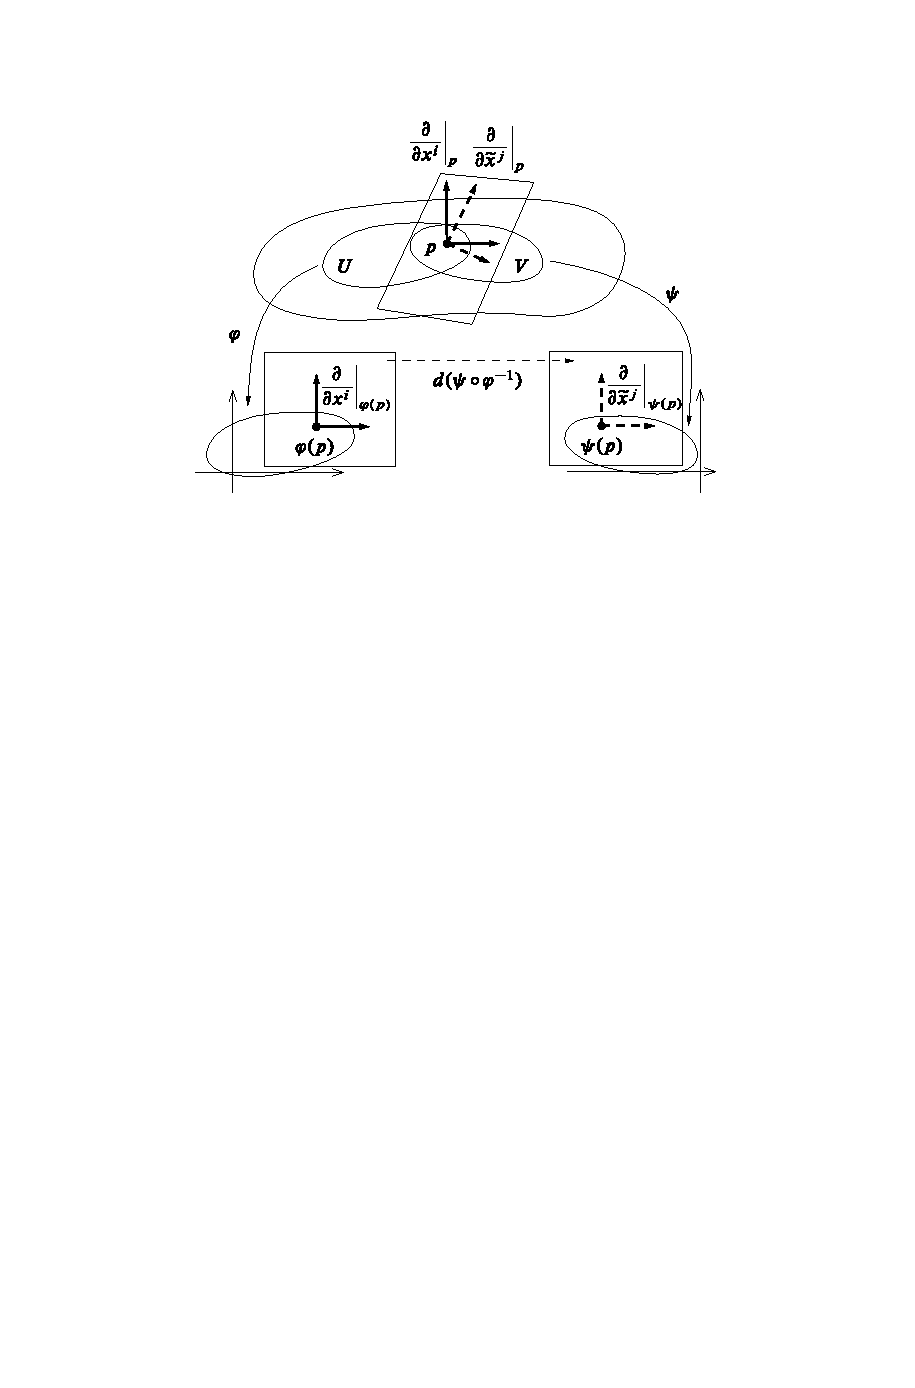
\includegraphics{pictures/coordinate-change}
    \caption{Change of coordinates.}
\end{figure}

In this situation, it is customary to write the transition map $\psi\circ\varphi^{-1}:\varphi(U\cap V)\to\psi(U\cap V)$ in the following shorthand notation:
\[\psi\circ\varphi^{-1}(x)=\big(\widetilde{x}^1(x),\dots,\widetilde{x}^n(x)\big)\]
The differential $d(\psi\circ\varphi^{-1})_{\varphi(p)}$ can be written
\[d(\psi\circ\varphi^{-1})_{\varphi(p)}\Big(\frac{\partial}{\partial x^i}\Big|_{\varphi(p)}\Big)=\frac{\partial\widetilde{x}^j}{\partial x^i}(\varphi(p))\frac{\partial}{\partial\widetilde{x}^j}\Big|_{\psi(p)}\]

Using the definition of coordinate vectors, we obtain
\begin{align*}
\frac{\partial}{\partial x^i}\Big|_p&=d(\varphi^{-1})\Big(\frac{\partial}{\partial x^i}\Big|_{\varphi(p)}\Big)=d(\psi^{-1})_{\psi(p)}\circ d(\psi\circ\varphi^{-1})_{\varphi(p)}\Big(\frac{\partial}{\partial x^i}\Big|_{\varphi(p)}\Big)\\
&=\frac{\partial\widetilde{x}^j}{\partial x^i}(\varphi(p))d(\psi^{-1})_{\psi(p)}\frac{\partial}{\partial\widetilde{x}^j}\Big|_{\psi(p)}\\
&=\frac{\partial\widetilde{x}^j}{\partial x^i}(\varphi(p))\frac{\partial}{\partial\widetilde{x}^j}\Big|_{p}.
\end{align*}
Applying this to the components of a vector $v=v^i\partial/\partial x^i|_p=\widetilde{v}^j\partial/\partial\widetilde{x}^j|_p$, we find that the components of $v$ transform by the rule
\begin{align}\label{coordinate change-1}
\widetilde{v}^j=v^i\frac{\partial\widetilde{x}^j}{\partial x^i}(\widehat{p})
\end{align}
\begin{example}
The transition map between polar coordinates and standard coordinates
in suitable open subsets of the plane is given by $(x,y)=(r\cos\theta,r\sin\theta)$. Let $p$ be the point in $\R^2$ whose polar coordinate representation is $(r,\theta)=(2,\pi/2)$, and let $v\in T_p\R^2$ be the tangent vector whose polar coordinate representation is 
\[v=3\frac{\partial}{\partial r}\Big|_p-\frac{\partial}{\partial\theta}\Big|_p\]
Applying the formula to the coordinate vectors, we find
\[\frac{\partial}{\partial r}\Big|_p=\cos\Big(\frac{\pi}{2}\Big)\frac{\partial}{\partial x}\Big|_p+\sin\Big(\frac{\pi}{2}\Big)\frac{\partial}{\partial y}\Big|_p=\frac{\partial}{\partial y}\Big|_p\]
\[\frac{\partial}{\partial\theta}\Big|_p=-2\sin\Big(\frac{\pi}{2}\Big)\frac{\partial}{\partial x}\Big|_p+2\cos\Big(\frac{\pi}{2}\Big)\frac{\partial}{\partial y}\Big|_p=-2\frac{\partial}{\partial x}\Big|_p\]
and thus $v$ has the following coordinate representation in standard coordinates:
\[v=3\frac{\partial}{\partial y}\Big|_p+2\frac{\partial}{\partial x}\Big|_p\]
\end{example}
\section{The tangent bundle}
Given a smooth manifold $M$ with or without boundary, we define the tangent bundle of $M$, denoted by $TM$, to be the disjoint union of the tangent spaces at all points of $M$:
\[TM=\coprod_{p\in M}T_pM\]
We usually write an element of this disjoint union as an ordered pair $(p,v)$, with $p\in M$ and $v\in T_pM$.
\begin{proposition}\label{tangent bundle struct}
For any smooth $n$-manifold $M$, the tangent bundle $TM$ has a natural topology and smooth structure that make it into a $2n$-dimensional smooth manifold. With respect to this structure, the projection $\pi:TM\to M$ is smooth.
\end{proposition}
\begin{proof}
We begin by defining the maps that will become our smooth charts. Given any smooth chart $(U,\varphi)$ for $M$, let $x^1,\dots,x^n$ denote the coordinate functions
of $\varphi$, and define a map $\tilde{\varphi}:\pi^{-1}(U)\to\R^{2n}$ by
\[\tilde{\varphi}\Big(v^i\frac{\partial}{\partial x^i}\Big|_p\Big)=(x^1(p),\dots,x^n(p),v^1,\dots,v^n)\]
Its image set is $\varphi(U)\times\R^n$, which is an open subset of $\R^{2n}$. It is a bijection onto its image, because its inverse can be written explicitly as
\[\tilde{\varphi}^{-1}(x^1,\dots,x^n,v^1,\dots,v^n)=v^i\frac{\partial}{\partial x^i}\Big|_{\varphi^{-1}(x)}\]
Now suppose we are given two smooth charts $(U,\varphi)$ and $(V,\psi)$ for $M$, and let $(\pi^{-1}(U),\tilde{\varphi})$ and $(\pi^{-1}(V),\tilde{\psi})$ be the corresponding charts on $TM$. The sets
\[\tilde{\varphi}\big(\pi^{-1}(U)\cap\pi^{-1}(V)\big)=\varphi(U\cap V)\times\R^n\And\tilde{\psi}\big(\pi^{-1}(U)\cap\pi^{-1}(V)\big)=\psi(U\cap V)\times\R^n\]
are open in $\R^{2n}$, and the transition map $\tilde{\psi}\circ\tilde{\varphi}^{-1}:\varphi(U\cap V)\times\R^n\to\psi(U\cap V)\times\R^n$ can be written explicitly as
\begin{align*}
\tilde{\psi}\circ\tilde{\varphi}^{-1}(x^1,\dots,x^n,v^1,\dots,v^n)&=\tilde{\psi}\Big(v^i\frac{\partial}{\partial x^i}\Big|_{\varphi^{-1}(x)}\Big)\\
&=\tilde{\psi}\Big(v^i\frac{\partial\widetilde{x}^j}{\partial x^i}\frac{\partial}{\partial \widetilde{x}^j}\Big|_{\varphi^{-1}(x)}\Big)\\
&=\big(\widetilde{x}^1(x),\dots,\widetilde{x}^n(x),v^i\frac{\partial\widetilde{x}^1}{\partial x^i}(x),\dots,v^i\frac{\partial\widetilde{x}^n}{\partial x^i}(x)\big)
\end{align*}
This is clearly smooth.\par
Choosing a countable cover $\{U_i\}$ of $M$ by smooth coordinate domains, we obtain a countable cover of $TM$ by coordinate domains $\{\pi^{-1}(U_i)\}$ satisfying conditions (\rmnum{1})--(\rmnum{4}) of the smooth manifold chart lemma. To check the Hausdorff condition (\rmnum{5}), just note that any two points in the same fiber of $\pi$ lie in one chart, while if $(p,v)$ and $(q,w)$ lie in different fibers, there exist disjoint smooth coordinate domains $U,V$ for $M$ such that $p\in U$ and $q\in V$, and then $\pi^{-1}(U)$ and $\pi^{-1}(V)$ are disjoint coordinate neighborhoods containing $(p,v)$ and $(q,w)$, respectively.\par
To see that $\pi$ is smooth, note that with respect to charts $(U,\varphi)$ for $M$ and $(\pi^{-1}(U),\tilde{\varphi})$ for $TM$, its coordinate representation is $\pi(x,v)=x$.
\end{proof}
The coordinates given by this proposition are called \textbf{natural coordinates} on $TM$.
\begin{proposition}
If $M$ is a smooth $n$-manifold with or without boundary, and $M$ can be covered by a single smooth chart, then $TM$ is diffeomorphic to $M\times\R^n$.
\end{proposition}
\begin{proof}
If $(U,\varphi)$ is a global smooth chart for $M$, then $\varphi$ is, in particular, a diffeomorphism from $U=M$ to an open subset $\widehat{U}\sub\R^n$ or $\H^n$. The proof of the previous proposition showed that the natural coordinate chart $\tilde{\varphi}$ is a bijection from $TM$ to $\widetilde{U}\times\R^n$, and the smooth structure on $TM$ is defined essentially by declaring $\tilde{\varphi}$ to be a diffeomorphism.
\end{proof}
\begin{remark}
In general, the tangent bundle is not globally diffeomorphic $($or even homeomorphic$)$ to a product of the manifold with $\R^n$.
\end{remark}
By putting together the differentials of $F$ at all points of $M$ we obtain a globally defined map between tangent bundles, called the \textbf{global differential} or global tangent map and denoted by $dF:TM\to TN$. This is just the map whose restriction to each tangent space $T_pM\sub TM$ is $dF_p$.\par
One important feature of the smooth structure we have defined on $TM$ is that it
makes the differential of a smooth map into a smooth map between tangent bundles.
\begin{proposition}
If $F:M\to N$ is a smooth map, then its global differential $dF:TM\to TN$ is a smooth map.
\end{proposition}
\begin{proof}
From the local expression for $dF_p$ in coordinates, it follows that $dF$ has the following coordinate representation in terms of natural coordinates for $TM$ and $TN$:
\begin{align*}
dF(x^1,\dots,x^n,v^1,\dots,v^n)=(F^1(x),\dots,F^n(x),v^i\frac{\partial F^1}{\partial x^i},\dots,v^i\frac{\partial F^n}{\partial x^i})
\end{align*}
This is smooth because $F$ is.
\end{proof}
\begin{proposition}
Suppose $F:M\to N$ and $G:N\to P$ are smooth maps.
\begin{itemize}
\item[(a)]$d(G\circ F)=dG\circ dF$.
\item[(b)]$d\id_M=\id_{TM}$.
\item[(c)]If $F$ is a diffeomorphism, then $dF:TM\to TN$ is also a diffeomorphism, and $d(F^{-1})=(dF)^{-1}$.
\end{itemize}
Because of part (c), when $F$ is a diffeomorphism we can use the notation $dF^{-1}$ unambiguously to mean either $d(F^{-1})$ or $(dF)^{-1}$.
\end{proposition}
\section{Velocity vectors of curves}
If $M$ is a manifold with or without boundary, we define a \textbf{curve} in $M$ to be a continuous map $\gamma:J\to M$, where $J\sub\R$ is an interval. Given a smooth
curve $\gamma:J\to M$ and $t_0\in J$ we define the \textbf{velocity} of $\gamma$ at $t_0$, denoted by $\gamma'(t_0)$, to be the vector
\[\gamma'(t_0)=d\gamma\Big(\frac{d}{dt}\Big|_{t_0}\Big)\in T_{\gamma(t_0)}M\]
where $d/dt|_{t_0}$ is the standard coordinate basis vector in $T_{t_0}\R$. This tangent vector acts on functions by
\[\gamma'(t_0)f=d\gamma\Big(\frac{d}{dt}\Big|_{t_0}\Big)f=\frac{d}{dt}\Big|_{t_0}(f\circ\gamma)=(f\circ\gamma)'(t_0)\]
In other words, $\gamma'(t_0)$ is the derivation at $\gamma(t_0)$ obtained by taking the derivative of a function along $\gamma$.\par
Now let $(U,\varphi)$ be a smooth chart with coordinate functions $(x^i)$. If $\gamma(t_0)\in U$, we can write the coordinate representation of $\gamma$ as $(\gamma^1(t),\dots,\gamma^n(t))$, at least for $t$ sufficiently close to $t_0$, and then the coordinate formula for the differential yields
\[\gamma'(t_0)=\frac{d\gamma^i}{dt}(t_0)\frac{\partial}{\partial x^i}\Big|_{\gamma(t_0)}\]
The next proposition shows that every tangent vector on a manifold is the velocity
vector of some curve. This gives a different and somewhat more geometric way to think about the tangent bundle: it is just the set of all velocity vectors of smooth
curves in $M$.
\begin{proposition}
Suppose $M$ is a smooth manifold with or without boundary and $p\in M$. Every $v\in T_pM$ is the velocity of some smooth curve in $M$.
\end{proposition}
\begin{proof}
First suppose that $p\in\Int M$ (which includes the case $\partial M=\emp$). Let $(U,\varphi)$ be a smooth coordinate chart centered at $p$, and write $v=v^i\partial/\partial x^i|_p$ in terms of the coordinate basis. For sufficiently small $\eps>0$, let $\gamma:(-\eps,\eps)\to U$ be the curve whose coordinate representation is
\[\gamma(t)=(tv^1,\dots,tv^n)\]
This is a smooth curve with $\gamma(0)=p$, and the computation above shows that $\gamma'(0)=v^i\partial/\partial x^i|_{\gamma(0)}=v$.\par
Now suppose $p\in\partial M$. Let $(U,\varphi)$ be a smooth boundary chart centered at $p$, and write $v=v^i\partial/\partial x^i|_p$. We wish to let $\gamma$ as before, but this formula represents a point of $M$ only when $tv^n\geq 0$. We can accommodate this requirement by suitably restricting the domain of $\gamma$: if $v_n=0$, we define $\gamma:(-\eps,\eps)\to U$ as before; if $v_n>0$, we let the domain be $[0,\eps)$ and if $v_n<0$, we let it be $(-\eps,0]$. In each case, $\gamma$ is a smooth curve in $M$ with $\gamma(0)=v$ and $\gamma'(0)=v$.
\end{proof}
\begin{proposition}[\textbf{The Velocity of a Composite Curve}]\label{diff composite curve}
Let $F:M\to N$ be a smooth map, and let $\gamma:J\to M$ be a smooth curve. For any $t_0\in J$, the velocity at $t=t_0$ of the composite curve $F\circ\gamma:J\to N$ is given by
\[(F\circ\gamma)'(t_0)=dF(\gamma'(t_0))\]
\end{proposition}
\begin{proof}
\[(F\circ\gamma)'(t_0)=d(F\circ\gamma)\Big(\frac{d}{dt}\Big|_{t_0}\Big)=dF\circ d\gamma\Big(\frac{d}{dt}\Big|_{t_0}\Big)=dF(\gamma'(t_0))\]
\end{proof}
\begin{corollary}[\textbf{Computing the Differential Using a Velocity Vector}]\label{compute diff by curve}
Suppose $F:M\to N$ is a smooth map, $p\in M$, and $v\in T_pM$. Then
\[dF_p(v)=(F\circ\gamma)'(0)\]
for any smooth curve $\gamma:J\to M$ such that $0\in J$, $\gamma(0)=p$ and $\gamma'(0)=v$.
\end{corollary}
\section{Tangent vectors as derivations of the space of germs}
A \textbf{smooth function element} on $M$ is an ordered pair $(f,U)$, where $U$ is an open subset of $M$ and $f:U\to\R$ is a smooth function. Given a point $p\in M$, we define an equivalence relation on the set of all smooth function elements whose domains contain $p$ by setting $(f,U)\sim (g,V)$ if $f=g$ on some neighborhood of $p$. The equivalence class of a function element $(f,U)$ is called the \textbf{germ} of $f$ at $p$, which we denote by $[f]_p$. The set of all germs of smooth functions at $p$ is denoted by $C^\infty_p(M)$. It is a vector space.\par
A derivation of $C^\infty_p(M)$ is a linear map $v:C^\infty_p(M)\to\R$ satisfying the following product rule
\[v[fg]_p=fv[g]_p+gv[f]_p.\]
It is common to define the tangent space to $M$ at $p$ as the vector space $\mathcal{D}_pM$ of derivations of $C^\infty_p(M)$. By proposition~\ref{tangent space local} $\mathcal{D}_pM$ is naturally isomorphic to the tangent space as we have defined.
\section{Exercise}
\begin{exercise}
Suppose $M$ and $N$ are smooth manifolds with or without boundary, and $F:M\to N$ is a smooth map. Show that $dF_p:T_pM\to T_{F(p)}N$ is the zero map for each $p\in M$ if and only if $F$ is constant on each component of $M$.
\end{exercise}
\begin{proof}
If $F$ is contant on each component of $M$, then $dF_p$ is zero by a coordinate computation. Assume the converse, let
\[\mathscr{C}=\{p\in M:\text{there is a neighborhood $U$ of $p$ such that $F$ is constant on $U$}\}\]
Then by continuity $\mathscr{C}$ is closed, and by pull back to Euclidean space, $\mathscr{C}$ is open. Hence $\mathscr{C}$ is a component.
\end{proof}
\begin{exercise}
Prove that if $M$ and $N$ are smooth manifolds, then $T(M\times N)$ is diffeomorphic
to $TM\times TN$.
\end{exercise}
\begin{exercise}
Let $S^1\sub\R^2$ be the unit circle, and let $K\sub\R^2$ be the boundary of the square of side $2$ centered at the origin: $K=\{(x,y):\max\{|x|,|y|\}\leq 1\}$. Show that there is a homeomorphism $F:\R^2\to\R^2$ such that $F(S^1)=K$, but there is
no diffeomorphism with the same property.
\end{exercise}
\begin{proof}
The projection from $S^1$ to $K$ is a homeomorphism. Suppose there is a diffeomorphism with the same property. let $\gamma:(-1,1)\to S^1$ be a smooth curve whose image lies in $S^1$ and such that $\gamma'(t)\neq 0$. Then since $F$ is a diffeomorphism, $dF(\gamma'(t))\neq 0$ for all $t$.
\[dF(\gamma'(t))(x)=\gamma'(t)(x\circ F)=\gamma'(t)F_1=(F_1\circ\gamma)'(t)\]
\[dF(\gamma'(t))(y)=\gamma'(t)(x\circ F)=\gamma'(t)F_1=(F_2\circ\gamma)'(t)\]
We choose $\gamma$ such that $F\circ\gamma(0)=(1,1)$, then $0$ is a critical point of $F\circ\gamma$, hence $(F_2\circ\gamma)'(0)=(F_2\circ\gamma)'(0)=0$. This is a contradiction since $dF(\gamma'(0))\neq 0$.
\end{proof}
\chapter{Submersions, immersions, and embeddings}
\section{Maps of constant rank}
Suppose $M$ and $N$ are smooth manifolds with or without boundary. Given a smooth map $F:M\to N$ and a point $p\in M$, we define the \textbf{rank of $\bm{F}$ at $\bm{p}$} to be the rank of the linear map $dF_p:T_pM\to T_{F(p)}N$, it is the rank of the Jacobian matrix of $F$ in any smooth chart, or the dimension of $\im dF_p\sub T_{F(p)}N$. If $F$ has the same rank $r$ at every point, we say that it has constant rank, and write $\rank(F)=r$.\par
Because the rank of a linear map is never higher than the dimension of either its domain or its codomain, the rank of $F$ at each point is bounded above by the minimum of $\{\dim(M), \dim(N)\}$. If the rank of $dF_p$ is equal to this upper bound, we say that \textbf{$\bm{F}$ has full rank at $\bm{p}$}, and if $F$ has full rank everywhere, we say \textbf{$\bm{F}$ has full rank}.\par
The most important constant-rank maps are those of full rank. A smooth map $F:M\to N$ is called a smooth \textbf{submersion} if its differential is surjective at each point (or equivalently, if $\rank(F)=\dim(N)$ everywhere). It is called a smooth \textbf{immersion} if its differential is injective at each point (equivalently, $\rank(F)=\dim(M)$ everywhere).\par
\begin{proposition}\label{local immersion subm}
Suppose $F:M\to N$ is a smooth map and $p\in M$.
\begin{itemize}
\item[(a)] If $dF_p$ is surjective, then $p$ has a neighborhood $U$ such that $F|_U$ is a submersion.
\item[(b)] If $dF_p$ is injective, then $p$ has a neighborhood $U$ such that $F|_U$ is an immersion.
\end{itemize}
\end{proposition}
\begin{proof}
If we choose any smooth coordinates for $M$ near $p$ and for $N$ near $F(p)$, either hypothesis means that Jacobian matrix of $F$ in coordinates has full rank at $p$. Example~\ref{full rank mani} shows that the set of $m\times n$ matrices of full rank is an open subset of $\mathcal{M}_{mn}(\R)$ (where $m=\dim(M)$ and $n=\dim(N)$), so by continuity, the Jacobian of $F$ has full rank in some neighborhood of $p$.
\end{proof}
\subsection{Local diffeomorphisms}
If $M$ and $N$ are smooth manifolds with or without boundary, a map $F:M\to N$ is called a \textbf{local diffeomorphism} if every point $p\in M$ has a neighborhood $U$ such that $F(U)$ is open in $N$ and $F:U\to F(U)$ is a diffeomorphism. The next theorem is the key to the most important properties of local diffeomorphisms.
\begin{theorem}[\textbf{Inverse Function Theorem for Manifolds}]
Suppose $M$ and $N$ are smooth manifolds, and $F:M\to N$ is a smooth map. If $p\in M$ is a point such that $dF_p$ is invertible, then there are connected neighborhoods $U_0$ of $p$ and $V_0$ of $F(p)$ such that $F|_{U_0}:U_0\to V_0$ is a diffeomorphism.
\end{theorem}
\begin{proof}
The fact that $dF_p$ is bijective implies that $M$ and $N$ have the same dimension, say $n$. Choose smooth charts $(U,\varphi)$ centered at $p$ and $(V,\psi)$ centered at $F(p)$, with $F(U)\sub V$. Then $\widehat{F}=\psi\circ F\circ\varphi^{-1}$ is a smooth map from the open subset $\widehat{U}\sub\R^n$ into $\widehat{V}\sub\R^n$, with $\widehat{F}(0)=0$. Because $\varphi$ and $\psi$ are diffeomorphisms, the differential $d\widehat{F}_0=d\psi_{F(p)}\circ dF_p\circ d\varphi^{-1}_0$ is nonsingular. The ordinary inverse function theorem shows that there are connected open subsets $\widehat{U}_0$ and $\widehat{V}_0$ containing $0$ such that $\widehat{F}$ restricts to a diffeomorphism from $\widehat{U}_0$ to $\widehat{V}_0$. Then $U_0=\varphi^{-1}(\widehat{U}_0)$ and $V_0=\psi^{-1}(\widehat{V}_0)$ are connected neighborhoods of $p$ and $F(p)$, respectively, and it follows by composition that $F|_{U_0}$ is a diffeomorphism from $U_0$ to $V_0$.
\end{proof}
\begin{proposition}[\textbf{Elementary Properties of Local Diffeomorphisms}]\label{local diff prop}
\mbox{}
\begin{itemize}
\item[(a)] Every composition of local diffeomorphisms is a local diffeomorphism.
\item[(b)] Every finite product of local diffeomorphisms between smooth manifolds is a local diffeomorphism.
\item[(c)] Every local diffeomorphism is a local homeomorphism and an open map.
\item[(d)] The restriction of a local diffeomorphism to an open submanifold with or without boundary is a local diffeomorphism.
\item[(e)] Every diffeomorphism is a local diffeomorphism.
\item[(f)] Every bijective local diffeomorphism is a diffeomorphism.
\item[(g)] A map between smooth manifolds with or without boundary is a local diffeomorphism if and only if in a neighborhood of each point of its domain, it has a
coordinate representation that is a local diffeomorphism.
\end{itemize}
\end{proposition}
\begin{proof}
We only prove (f). Let $F:M\to N$ be a bijective local diffeomorphism, and $F^{-1}$ be its inverse. For each $p\in M$, there are neighborhood $U_p$ of $p$ and $V_p$ of $F(p)$ such that $F|_{U_p}:U_p\to V_p$ is a diffeomorphism. Then from the uniqueness of an inverse function we get $(F|_{U_p})^{-1}=F^{-1}|_{V_p}$. Now since $F$ is surjective, every point in $N$ has a neighborhood on which $F^{-1}$ is a smooth function, hence $F^{-1}$ is smooth and $F$ is a diffeomorphism.
\end{proof}
\begin{proposition}\label{local diff iff}
Suppose $M$ and $N$ are smooth manifolds $($without boundary$)$, and $F:M\to N$ is a map.
\begin{itemize}
\item[(a)] $F$ is a local diffeomorphism if and only if it is both a smooth immersion and a smooth submersion.
\item[(b)] If $\dim(M)=\dim(N)$ and $F$ is either a smooth immersion or a smooth submersion, then it is a local diffeomorphism.
\end{itemize}
\end{proposition}
\begin{proof}
Suppose first that $F$ is a local diffeomorphism. Given $p\in M$, there is a neighborhood $U$ of $p$ such that $F$ is a diffeomorphism from $U$ to $F(U)$. It then follows from Proposition~\ref{differential mani prop} that $dF_p:T_pM\to T_{F(p)}N$ is an isomorphism. Thus $\rank(F)=\dim(M)=\dim(N)$, so $F$ is both a smooth immersion and a smooth submersion. Conversely, if $F$ is both a smooth immersion and a smooth submersion, then $dF_p$ is an isomorphism at each $p\in M$, and the inverse function theorem for manifolds shows that $p$ has a neighborhood on which $F$ restricts to a diffeomorphism onto its image. This proves (a).\par
To prove (b), note that if $M$ and $N$ have the same dimension, then either injectivity or surjectivity of $dF_p$ implies bijectivity, so $F$ is a smooth submersion if and only if it is a smooth immersion, and thus (b) follows from (a).
\end{proof}
\begin{proposition}\label{smooth iff composition smooth}
Suppose $M,N,P$ are smoothmanifolds with or without boundary, and $F:M\to N$ is a local diffeomorphism.
\begin{itemize}
\item[(a)]If $G:P\to M$ is continuous, then $G$ is smooth if and only if $F\circ G$ is smooth.
\item[(b)]If in addition $F$ is surjective and $G:N\to P$ is any map, then $G$ is smooth if and only if $G\circ F$ is smooth.
\end{itemize}
\begin{proof}
For part (a), we assume that $F\circ G$ is smooth. For any point $p\in P$, we can choose neighborhood $U$ for $G(p)$ such that $F|_U:U\to F(U)$ is a diffeomorphism. Then $\widetilde{U}:=G^{-1}(U)$ is a neighborhood of $p$ since $G$ is continuous, and we have
\[G|_{\widetilde{U}}=(F|_{U})^{-1}\circ (G\circ F)|_{\widetilde{U}}\]
Thus as a compoistion of smooth maps, $G|_{\widetilde{U}}$ is smooth. It follows that $G$ itself is smooth.\par
For part (b), assume that $G\circ F$ is smooth. For each point $p\in N$, choose $x\in F^{-1}(p)$. Then we can find neighborhood $U$ containting $x$ and $V$ containting $p$ such that $F$ is a diffeomorphism from $U$ to $V$. Then
\[G|_V=(G\circ F)_U\circ(F|U)^{-1}\]
Thus $G|_V$ is smooth, and hence $G$ is smooth.
\end{proof}
\end{proposition}
\subsection{The rank theorem}
\begin{theorem}[\textbf{Rank Theorem}]
Suppose $M$ and $N$ are smooth manifolds of dimensions $m$ and $n$, respectively, and $F:M\to N$ is a smooth map with constant rank $r$. For each $p\in M$ there exist smooth charts $(U,\varphi)$ for $M$ centered at $p$ and $(V,\psi)$ for $N$ centered at $F(p)$ such that $F(U)\sub V$, in which $F$ has a coordinate representation of the form
\begin{align}\label{Rank thm mani-1}
\widehat{F}(x^1,\dots,x^r,x^{r+1},\dots,x^m)=(x^1,\dots,x^r,0,\dots,0)
\end{align}
In particular, if $F$ is a smooth submersion, this becomes
\[\widehat{F}(x^1,\dots,x^n,x^{n+1},\dots,x^m)=(x^1,\dots,x^n)\]
and if $F$ is a smooth immersion, it is
\[\widehat{F}(x^1,\dots,x^m)=(x^1,\dots,x^m,0,\dots,0)\]
\end{theorem}
\begin{proof}
Since the question is local, we can assume that $M$ and $N$ are open subsets of Euclidean spaces. The theorem then follows from Theorem~\ref{rank theorem}.
\end{proof}
The next corollary can be viewed as a more invariant statement of the rank theorem. It says that constant-rank maps are precisely the ones whose local behavior is the same as that of their differentials.
\begin{corollary}
Let $M$ and $N$ be smooth manifolds, let $F:M\to N$ be a smooth map, and suppose $M$ is connected. Then the following are equivalent:
\begin{itemize}
\item[(a)]For each $p\in M$ there exist smooth charts containing $p$ and $F(p)$ in which the coordinate representation of $F$ is linear.
\item[(b)]$F$ has constant rank.
\end{itemize}
\end{corollary}
\begin{proof}
First suppose $F$ has a linear coordinate representation in a neighborhood of each point. Since every linear map has constant rank, it follows that the rank of $F$ is
constant in a neighborhood of each point, and thus by connectedness it is constant
on all of $M$. Conversely, if $F$ has constant rank, the rank theorem shows that it has the linear coordinate representation in a neighborhood of each point.
\end{proof}
The rank theorem is a purely local statement. However, it has the following powerful
global consequence.
\begin{theorem}[\textbf{Global Rank Theorem}]\label{global rank thm}
Let $M$ and $N$ be smooth manifolds, and suppose $F:M\to N$ is a smooth map of constant rank.
\begin{itemize}
\item[(a)]If $F$ is surjective, then it is a smooth submersion.
\item[(b)]If $F$ is injective, then it is a smooth immersion.
\item[(c)]If $F$ is bijective, then it is a diffeomorphism.
\end{itemize}
\end{theorem}
\begin{proof}
Let $m=\dim(M)$, $n=\dim(N)$, and suppose $F$ has constant rank $r$. To prove (a), assume that $F$ is not a smooth submersion, which means that $r<n$. By the rank theorem, for each $p\in M$ there are smooth charts $(U,\varphi)$ for $M$ centered
at $p$ and $(V,\psi)$ for $N$ centered at $F(p)$ such that $F(U)\sub V$ and the coordinate representation of $F$ is given by $(\ref{Rank thm mani-1})$. Shrinking $U$ if necessary, we may assume that it is a regular coordinate ball and $F(\widebar{U})\sub V$. This implies that $F(\widebar{U})$ is a compact subset of the set $\{y\in V:y^{r+1}=\cdots=y^n=0\}$, so it is closed in $N$ and contains no open subset of $N$; hence is nowhere dense in $N$. Since every open cover of a manifold has a countable subcover, we can choose countably many such charts $\{U_i\}$ covering $M$, with corresponding charts $\{V_i\}$ covering $F(M)$. Because $F(M)$ is equal to the countable union of the nowhere dense sets $F(\widebar{U}_i)$, it follows from the Baire category theorem that $F(M)$ has empty interior in $N$, which means $F$ cannot be surjective.\par
To prove (b), assume that $F$ is not a smooth immersion, so that $r<m$. By the rank theorem, for each $p\in M$ we can choose charts on neighborhoods of $p$ and $F(p)$ in which $F$ has the coordinate representation of $(\ref{Rank thm mani-1})$. It follows that 
\[F(0,\dots,0,\eps)=(0,\dots,0)=F(0,\dots,0)\]
for any sufficiently small $\eps$, so $F$ is not injective.\par
Finally, (c) follows from (a) and (b), because a bijective smooth map of constant rank is a smooth submersion by part (a) and a smooth immersion by part (b); so Proposition~\ref{local diff iff} implies that $F$ is a local diffeomorphism, and because it is bijective, it is a diffeomorphism.
\end{proof}
\subsection{The rank theorem for manifolds with boundary}
In the context of manifolds with boundary, we need the rank theorem only in one special case: that of a smooth immersion whose domain is a smooth manifold with boundary. Of course, since the interior of a smooth manifold with boundary is a smooth manifold, near any interior point of the domain the ordinary rank theorem applies. For boundary points, we have the following substitute for the rank theorem.
\begin{theorem}[\textbf{Immersion Theorem for Manifolds with Boundary}]\label{rank thm manifold boundary}
Let $M$ be a smooth $m$-manifold with boundary, $N$ be a smooth $n$-manifold, and $F:M\to N$ be a smooth immersion. For any $p\in\partial M$, there exist a smooth boundary chart $(U,\varphi)$ for $M$ centered at $p$ and a smooth coordinate chart $(V,\psi)$ for $N$ centered at $F(p)$ with $F(U)\sub V$, in which $F$ has the coordinate representation
\begin{align}\label{rank thm boundary-1}
\widehat{F}(x^1,\dots,x^m)=(x^1,\dots,x^m,0,\dots,0)
\end{align}
\end{theorem}
\begin{proof}
By choosing initial smooth charts for $M$ and $N$, we may assume that $M$ and $N$ are open subsets of $\H^m$ and $\R^n$, respectively, and also that $p=0\in\H^m$, and $F(p)=0\in\R^n$. By definition of smoothness for functions on $\H^m$, $F$ extends to a smooth map $\widetilde{F}:W\to\R^n$, where $W$ is some open subset of $\R^m$ containing $0$. Because $d\widetilde{F}_0=dF$ is injective, by Proposition~\ref{local immersion subm} we may assume that $\widetilde{F}$ is a smooth immersion. Let us write the coordinates on $\R^m$ as $x=(x^1,\dots,x^m)$, and those on $\R^n$ as $(v,w)=(v^1,\dots,v^m,w^1,\dots,w^{n-m})$.\par
By the rank theorem, there exist smooth charts $(U_0,\varphi_0)$ for $\R^m$ centered at $0$ and $(V_0,\psi_0)$ for $\R^n$ centered at $0$ such that $\widehat{F}=\psi_0\circ\widetilde{F}\circ\varphi^{-1}_0$ is given by $(\ref{rank thm boundary-1})$. The only problem with these coordinates is that $\varphi$ might not restrict to a boundary chart for $M$. But we can correct this easily as follows. Because $\varphi_0$ is a diffeomorphism from $U_0$ to an open subset $\widehat{U}_0=\varphi_0(U_0)\sub\R^m$, the map $\varphi_0^{-1}\times\mathrm{id}_{\R^{n-m}}$ is a diffeomorphism from $\widehat{U}_0\times\R^{n-m}$ to $U_0\times\R^{n-m}$. Let $\psi=(\varphi_0^{-1}\times\mathrm{id}_{\R^{n-m}})\circ\psi_0$, which is a diffeomorphism from some open subset $V\sub V_0$ containing $0$ to a neighborhood
of $0$ in $\R^n$. Using $(\ref{rank thm boundary-1})$, we compute
\begin{align*}
\psi\circ F(x)&=(\varphi_0^{-1}\times\mathrm{id}_{\R^{n-m}})\circ\psi_0\circ F\circ\varphi_0^{-1}\circ\varphi_0(x)=(\varphi_0^{-1}\times\mathrm{id}_{\R^{n-m}})\circ\widehat{F}(\varphi_0(x))\\
&=(\varphi_0^{-1}\times\mathrm{id}_{\R^{n-m}})(\varphi_0(x),0)=(x,0)
\end{align*}
Thus, the original coordinates for $M$ (restricted to a sufficiently small neighborhood of $0$) and the chart $(V,\psi)$ for $N$ satisfy the desired conditions.
\end{proof}
It is possible to prove a similar theorem for more general maps with constant rank out of manifolds with boundary, but the proof is more elaborate because an extension of $F$ to an open subset does not automatically have constant rank (Recall Example~\ref{rank function}).
\begin{corollary}\label{rank thm boundary}
Suppose $M$ is a smooth $m$-manifold with boundary, $N$ is a smooth $n$-manifold, and
$F:M\to N$ has constant rank $r$. If for any $p\in\partial M$ we have$\ker dF_p\nsubseteq T_p\partial M$, then for each $p$ there exist a smooth boundary chart $(U,\varphi)$ for $M$ centered at $p$ and a smooth coordinate chart $(V,\psi)$ for $N$ centered at $F(p)$ with $F(U)\sub V$, in which $F$ has the coordinate representation
\begin{align}\label{rank thm boundary-2}
\widehat{F}(x^1,\dots,x^r,x^{r+1},\dots,x^m)=(x^1,\dots,x^r,0,\dots,0)
\end{align}
\end{corollary}
\begin{proof}
Choosing coooredinates as in the previous theorem, we can assume $M\sub\H^m$ and $N\sub\R^n$, also $p=0\in\H^m$ and $F(p)=0\in\R^n$. Now extend $F$ to a smooth function $\widetilde{F}:W\to\R^n$, where $W$ is an open subset of $\R^m$ containing $0$. there is a coordinate projection $\pi:\R^n\to\R^r$ such that $\pi\circ\widetilde{F}$ is a submersion. Now from the proof of Theorem~\ref{rank theorem}, we can see there is $\varphi:U_0\to\R^m$ such that
\[\pi\circ\widetilde{F}\circ\varphi^{-1}(x,y)=x\]
Thus we write $\widetilde{F}\circ\varphi^{-1}=(x,R(x,y))$. Then $R|_M$ is independent of $y$, so $\psi(v,w)=(v,w-R(v))$ gives the result.
\end{proof}
\section{Embeddings}
One special kind of immersion is particularly important. If $M$ and $N$ are smooth
manifolds with or without boundary, a \textbf{smooth embedding} of $M$ into $N$ is a smooth immersion $F:M\to N$ that is also a topological embedding. \textit{A smooth embedding is a map that is both a topological embedding and a smooth immersion, not just a topological embedding that happens to be smooth.}
\begin{example}[\textbf{A Smooth Topological Embedding}]
The map $\gamma:\R\to\R^2$ given by $\gamma(t)=(t^3,0)$ is a smooth map and a topological embedding, but it is not a smooth embedding because $\gamma'(0)=0$.
\end{example}
\begin{example}[\textbf{The Figure-Eight Curve}]\label{figure eight}
Consider the curve $\beta:(-\pi,\pi)\to\R^2$ defined by
\[\beta(t)=(\sin 2t,\sin t)\]
Its image is a set that looks like a figure-eight in the plane,sometimes
called a \textbf{lemniscate}. It is easy to see that $\beta$ is an injective smooth immersion because $\beta'(t)$ never vanishes; but it is not a topological embedding, because its image is compact in the subspace topology, while its domain is not.
\end{example}
\begin{example}[\textbf{A Dense Curve on the Torus}]\label{dense curve torus}
Let $T^2=S^1\times S^1\sub\C^2$ denote the torus, and let $\alpha$ be any irrational number. The map $\gamma:\R\to T^2$ given by
\[\gamma(t)=(e^{2\pi it},e^{2\pi i\alpha t})\]
is a smooth immersion because $\gamma'(t)$ never vanishes. It is also injective, because $\gamma(t_1)=\gamma(t_2)$ implies that both $t_1-t_2$ and $\alpha(t_1-t_2)$ are integers, which is impossible unless $t_1=t_2$.\par
We claim that $\gamma(\R)$ is dense in $T^2$. In fact, each point in $T^2$ is of the form $(e^{2\pi it_1},e^{2\pi it_2})$, and we observe that for all $n,m\in\N$,
\[\gamma(t_1+m)=(e^{2\pi it_1},e^{2\pi i\alpha(t_1+m)})=(e^{2\pi it_1},e^{2\pi i[\alpha(t_1+m)+n]}),\]
so we only need to show $\{\alpha m+n\}$ is dense in $\R$. This is a result called Kronecker's approximation theorem.
\end{example}
The following proposition gives a few simple sufficient criteria for an injective immersion to be an embedding.
\begin{proposition}\label{smooth embedd if}
Suppose $M$ and $N$ are smooth manifolds with or without boundary, and $F:M\to N$ is an injective smooth immersion. If any of the following holds, then $F$ is a smooth embedding.
\begin{itemize}
\item[(a)] $F$ is an open or closed map.
\item[(b)] $F$ is a proper map.
\item[(c)] $M$ is compact.
\item[(d)] $M$ has empty boundary and $\dim(M)=\dim(N)$.
\end{itemize}
\end{proposition}
\begin{proof}
If $F$ is open or closed, then it is a topological embedding, so it is a smooth embedding. Either (b) or (c) implies that $F$ is closed. Finally, assume that $M$ has empty boundary and $\dim(M)=\dim(N)$ Then $dF_p$ is nonsingular everywhere, and by Exercise~\ref{smooth map not boundary} $F(M)\sub\Int N$. Proposition~\ref{local diff iff} shows that $F:M\to\Int N$ is a local diffeomorphism, so it is an open map. It follows that $F:M\to N$ is a composition of open maps $M\to\Int N\sub N$, so it is an embedding.
\end{proof}
\begin{theorem}[\textbf{Local Embedding Theorem}]\label{immersion local embedding}
Suppose $M$ and $N$ are smooth manifolds with or without boundary, and $F:M\to N$ is a smooth map. Then $F$ is a smooth immersion if and only if every point in $M$ has a neighborhood $U\sub M$ such that $F|_U:U\to N$ is a smooth embedding.
\end{theorem}
\begin{proof}
One direction is immediate: if every point has a neighborhood on which $F$ is a smooth embedding, then $F$ has full rank everywhere, so it is a smooth immersion.\par
Conversely, suppose $F$ is a smooth immersion, and let $p\in M$. We show first that $p$ has a neighborhood on which $F$ is injective. If $F(p)\notin\partial N$, then that there is a neighborhood $U_1$ of $p$ on which $F$ has a coordinate representation of the form $x\mapsto(x,0)$. It follows from this formula that $F|_{U_1}$ is injective. On the other hand, suppose $F(p)\in\partial N$, and let $(W,\psi)$ be any smooth boundary chart for $N$ centered at $F(p)$. If we let $U_0=F^{-1}(W)$, which is a neighborhood of $p$, and let $\iota:\H^n\to\R^n$ be the inclusion map, then the preceding argument can be applied to the composite map
$\iota\circ\psi\circ F|_{U_0}$ to show that $p$ has a neighborhood $U_1\sub U_0$ such that $\iota\circ\psi\circ F|_{U_0}$ is injective, from which it follows that $F|_{U_1}$ is injective.\par
Now let $p\in M$ be arbitrary, and let $U_1$ be a neighborhood of $p$ on which $F$ is
injective. There exists a precompact neighborhood $U$ of $p$ such that $\widebar{U}\sub U_1$. The restriction of $F$ to $\widebar{U}$ is an injective continuous map with compact domain, so it is a topological embedding by the closed map lemma. Because any restriction of a topological embedding is again a topological embedding, $F|_U$ is both a topological embedding and a smooth immersion, hence a smooth embedding.
\end{proof}
\section{Submersions}
One of the most important applications of the rank theorem is to vastly expand our
understanding of the properties of submersions. If $\pi:M\to N$ is any continuous
map, a \textbf{section} of $\pi$ is a continuous right inverse for $\pi$, i.e., a continuous map $\sigma:N\to M$ such that $\pi\circ\sigma=\mathrm{id}_N$:
\[\begin{tikzcd}
M\ar[d,swap,"\pi"]\\
N\ar[u,swap,bend right=40,"\sigma"]
\end{tikzcd}\]
A \textbf{local section} of $\pi$ is a continuous map $\sigma:U\to M$ defined on some open subset $U\sub N$ and satisfying the analogous relation $\pi\circ\sigma=\mathrm{id}_U$. Many of the important properties of smooth submersions follow from the fact that they admit an abundance of smooth local sections.
\begin{theorem}[\textbf{Local Section Theorem}]\label{submersion iff local section}
Let $M$ and $N$ be smooth manifolds and $\pi:M\to N$ be a smooth map. Then $\pi$ is a smooth submersion if and only if every point of $M$ is in the image of a smooth local section of $\pi$.
\end{theorem}
\begin{proof}
First suppose that $\pi$ is a smooth submersion. Given $p\in M$, let $q=\pi(p)\in N$. By the rank theorem, we can choose smooth coordinates $(x^1,\dots,x^m)$ centered at $p$ and $(y^1,\dots,y^n)$ centered at $q$ in which $\pi$ has the coordinate representation
\[\pi(x^1,\dots,x^n,x^{n+1},\dots,x^m)=(x^1,\dots,x^n).\]
If $\eps$ is a sufficiently small positive number, the coordinate cube
\[C_\eps=\{x:|x^i|<\eps\}\sub\R^m\]
is a neighborhood of $p$ whose image under $\pi$ is the cube
\[C'_\eps=\{x:|x^i|<\eps\}\sub\R^n\]
The map $\sigma:C'_\eps\to C_\eps$ whose coordinate representation is
\[\sigma(x^1,\dots,x^n)=(x^1,\dots,x^n,0,\dots,0)\]
is a smooth local section of $\pi$ satisfying $\sigma(q)=p$. Conversely, assume each point of $M$ is in the image of a smooth local section. Given $p\in M$, let $\sigma:U\to M$ be a smooth local section such that $\sigma(q)=p$, where $q=\pi(p)\in N$. The equation $\pi\circ\sigma=\mathrm{id}_U$ implies that $d\pi_p\circ d\sigma_q=\mathrm{id}_{T_pN}$, which in turn implies that $d\pi_p$ is surjective.
\end{proof}
This theorem motivates the following definition: if $\pi:X\to Y$ is a continuous
map, we say $\pi$ is a \textbf{topological submersion} if every point of $X$ is in the image of a (continuous) local section of $\pi$. The preceding theorem shows that every smooth submersion is a topological submersion.
\begin{proposition}\label{smooth subm prop}
Let $M$ and $N$ be smooth manifolds, and suppose $\pi:M\to N$ is a smooth submersion. Then $\pi$ is an open map, and if it is surjective it is a quotient map.
\end{proposition}
\begin{proof}
Suppose $W$ is an open subset of $M$ and $q$ is a point of $\pi(W)$. For any $p\in W$
such that $\pi(p)=q$, there is a neighborhood $U$ of $q$ on which there exists a smooth local section $\sigma:U\to M$ satisfying $\sigma(q)=p$. For each $y\in\sigma^{-1}(W)$ the fact that $\sigma(y)\in W$ implies $y=\pi(\sigma(y))\in\pi(W)$. Thus $\sigma^{-1}(W)$ is a neighborhood of $q$ contained in $\pi(W)$, which implies that $\pi(W)$ is open. The second assertion follows from the first because every surjective open continuous map is a quotient map.
\end{proof}
We now state the following important theorems that are tools we will use frequently when studying submersions. This demonstrates that surjective smooth submersions play a role in smooth manifold theory analogous to the role of quotient maps in topology.
\begin{theorem}[\textbf{Characteristic Property of Surjective Submersions}]\label{manifold surjective submersion char}
Let $M$ and $N$ be smooth manifolds and $\pi:M\to N$ be a surjective smooth submersion. For any smooth manifold $P$ with or without boundary, a map $F:N\to P$ is smooth if and only if $F\circ\pi$ is smooth:
\[\begin{tikzcd}
M\ar[d,swap,"\pi"]\ar[rd,"F\circ\pi"]&\\
N\ar[r,swap,"F"]&P
\end{tikzcd}\]
\end{theorem}
\begin{proof}
If $F$ is smooth, then $F\circ\pi$ is smooth by composition. Conversely, suppose that $F\circ\pi$ is smooth, and let $q\in N$ be arbitrary. Since $\pi$ is surjective, there is a point $p\in\pi^{-1}(q)$ and then the local section theorem guarantees the existence of a neighborhood $U$ of $q$ and a smooth local section $\sigma:U\to M$ of $\pi$ such that $\sigma(q)=p$. Then $\pi\circ\sigma=\mathrm{id}_U$ implies
\[F|_U=F|_U\circ\mathrm{id}_U=F\circ(\pi\circ\sigma)=(F\circ\pi)\circ\sigma\]
which is a composition of smooth maps. This shows that $F$ is smooth in a neighborhood of each point, so it is smooth.
\end{proof}
The next theorem gives a very general sufficient condition under which a smooth map can be pushed down by a submersion.
\begin{theorem}[\textbf{Passing Smoothly to the Quotient}]\label{pass to quotient}
Suppose $M$ and $N$ are smooth manifolds and $\pi:M\to N$ is a surjective smooth submersion. If $P$ is a smooth manifold with or without boundary and $F:M\to P$ is a smooth map that is constant on the fibers of $\pi$, then there exists a unique smooth map $\widetilde{F}:N\to P$ such that $\widetilde{F}\circ\pi=F$:
\[\begin{tikzcd}
M\ar[d,swap,"\pi"]\ar[rd,"F"]&\\
N\ar[r,swap,dashed,"\widetilde{F}"]&P
\end{tikzcd}\]
\end{theorem}
\begin{proof}
Because a surjective smooth submersion is a quotient map, there exists a unique continuous map $\widetilde{F}:N\to P$ satisfying $\widetilde{F}\circ\pi=F$. It is smooth by Theorem~\ref{manifold surjective submersion char}.
\end{proof}
\begin{theorem}[\textbf{Uniqueness of Smooth Quotients}]\label{smooth quotient unique}
Let $\pi_1:M\to N_1$ and $\pi_2:M\to N_2$ be surjective smooth submersions that are constant on each other's fibers. Then there exists a unique diffeomorphism $F:N_1\to N_2$ such that $F\circ\pi_1=\pi_2$:
\[\begin{tikzcd}
&M\ar[ld,swap,"\pi_1"]\ar[rd,"\pi_2"]&\\
N_1\ar[rr,dashed,"F"]&&N_2
\end{tikzcd}\]
\end{theorem}
\begin{proof}
The existence of the continuous map $F$ and its inverse follow from the assumption of $\pi_1$ and $\pi_2$, and clearly $F\circ\pi_1=\pi_2$. The fact that $F$ is a diffeomorphism follows from the characterization Theorem~\ref{manifold surjective submersion char}.
\end{proof}
\section{Smooth covering maps}
In the context of smooth manifolds, it is useful to introduce a slightly more restrictive type of covering map. If $E$ and $M$ are connected smooth manifolds with
or without boundary, a map $\pi:E\to M$ is called a \textbf{smooth covering map} if $\pi$ is smooth and surjective, and each point in $M$ has a neighborhood $U$ such that each component of $\pi^{-1}(U)$ is mapped diffeomorphically onto $U$ by $\pi$. In this context we also say that $U$ is \textbf{evenly covered}. The space $M$ is called the \textbf{base of the covering}, and $E$ is called a \textbf{covering manifold} of $M$. If $E$ is simply connected, it is called the \textbf{universal covering manifold} of $M$.\par
To distinguish this new definition from the previous one, we often call an ordinary covering map a \textbf{topological covering map}. A smooth covering map is, in particular, a topological covering map. But a smooth covering map is more than just
a topological covering map that happens to be smooth: the definition requires in
addition that the restriction of $\pi$ to each component of the preimage of an evenly
covered set be a diffeomorphism, not just a smooth homeomorphism.
\begin{proposition}[\textbf{Properties of Smooth Coverings}]\label{smooth cover prop}
\mbox{}
\begin{itemize}
\item[(a)]Every smooth covering map is a local diffeomorphism, a smooth submersion,
an open map, and a quotient map.
\item[(b)]An injective smooth covering map is a diffeomorphism.
\item[(c)]A topological covering map is a smooth covering map if and only if it is a local diffeomorphism.
\end{itemize}
\end{proposition}
For smooth covering maps, the local section theorem can be strengthened.
\begin{theorem}[\textbf{Local Section for Smooth Covering Maps}]\label{local section unique}
Suppose $E$ and $M$ are smooth manifolds with or without boundary, and $\pi:E\to M$ is a smooth covering map. Given any evenly covered open subset $U\sub M$, any $q\in U$, and any $p$ in the fiber of $\pi$ over $q$, there exists a unique smooth local section $\sigma:U\to E$ such that $\sigma(q)=p$.
\end{theorem}
\begin{proof}
Suppose $U\sub M$ is evenly covered, $q\in U$, and $p\in\pi^{-1}(q)$. Let $\widetilde{U}$ be the component of $\pi^{-1}(q)$ containing $p$. Since the restriction of $\pi$ to $\widetilde{U}_0$ is a diffeomorphism onto $U$, the map  $\sigma=(\pi|_{\widetilde{U}_0})^{-1}$ is the required smooth local section.\par
To prove uniqueness, suppose $\sigma':U\to E$ is any other smooth local section satisfying $\sigma'(q)=p$. Since $U$ is connected, $\sigma'(U)$ is contained in the component $\widetilde{U}_0$ containing $p$. Because $\sigma'$ is a right inverse for the bijective map $\pi|_{U_0}$, it must be equal to its inverse, and therefore equal to $\sigma$.
\end{proof}
\begin{theorem}[\textbf{Covering Spaces of Smooth Manifolds}]\label{covering mani}
Suppose $M$ is a connected smooth $n$-manifold, and $\pi:E\to M$ is a topological covering map. Then $E$ is a topological $n$-manifold, and has a unique smooth structure such that $\pi$ is a smooth covering map.
\end{theorem}
\begin{proof}
Because $\pi$ is a local homeomorphism, $E$ is locally Euclidean. To show that it is Hausdorff, let $p_1$ and $p_2$ be distinct points in $E$. If $\pi(p_1)=\pi(p_2)$ and $U\sub M$ is an evenly covered open subset containing $\pi(p_1)$, then the components of $\pi^{-1}(U)$ containing $p_1$ and $p_2$ are disjoint open subsets of $E$ that separate $p_1$ and $p_2$. If $\pi(p_1)\neq\pi(p_2)$, there are disjoint open subsets $U_1,U_2\sub M$ containing $\pi(p_1)$ and $\pi(p_2)$, respectively, and then $\pi^{-1}(U_1)$ and $\pi^{-1}(U_2)$ are disjoint open subsets of $E$ containing $p_1$ and $p_2$. Thus $E$ is Hausdorff.\par
To show that $E$ is second-countable, we first note that the fundamental group of $X$ acts transitively on the fiber of $\pi$ and the fundamental group is countable, it follows that the fiber of $\pi$ is countable. The collection of all evenly covered open subsets is an open cover of $M$, and therefore has a countable subcover $\{U_i\}$. For any given $i$, each component of $\pi^{-1}(U_i)$ contains exactly one point in each fiber over $U_i$, so $\pi^{-1}(U_i)$ has countably many components. The collection of all components of all sets of the form $\pi^{-1}(U_i)$ is thus a countable open cover of $E$, since each such component is secondcountable, it follows that $E$ is second-countable. This completes the proof that $E$ is a topological manifold.\par
To construct a smooth structure on $E$, suppose $p$ is any point in $E$, and let $U$ be an evenly covered neighborhood of $\pi(p)$. After shrinking $U$ if necessary, we may assume also that it is the domain of a smooth coordinate map $\varphi:U\to\R^n$. If $\widetilde{U}$ is the component of $\pi^{-1}(U)$ containing $p$, and $\tilde{\varphi}=\varphi\circ\pi|_{\widetilde{U}}$, then $(\widetilde{U},\tilde{\varphi})$ is a chart on $E$. If two such charts $(\widetilde{U},\tilde{\varphi})$ and $(\widetilde{V},\tilde{\psi})$ overlap, the transition map can be written
\begin{align*}
\tilde{\psi}\circ\tilde{\varphi}^{-1}&=(\psi\circ\pi|_{\widetilde{U}\cap\widetilde{V}})\circ(\varphi\circ\pi|_{\widetilde{U}\cap\widetilde{V}})^{-1}\\
&=\psi\circ\varphi^{-1}
\end{align*}
which is smooth. Thus the collection of all such charts defines a smooth structure
on $E$.\par
Now let $(\widetilde{U}',\tilde{\varphi}')$ be another chart at $p$ such that $\pi$ is a smooth covering map with this chart. Then
\[\varphi\circ\pi\circ(\tilde{\varphi}')^{-1}=\tilde{\varphi}\circ(\tilde{\varphi}')^{-1}\]
is smooth, hence $(\widetilde{U}',\tilde{\varphi}')$ is equivalent to $(\widetilde{U},\tilde{\varphi})$.\par
Finally, $\pi$ is a smooth covering map because its coordinate representation in
terms of any pair of charts $(\widetilde{U},\tilde{\varphi})$ and $(U,\varphi)$ constructed above is the identity.
\end{proof}
\begin{corollary}[\textbf{Existence of a Universal Covering Manifold}]
If $M$ is a connected smooth manifold, there exists a simply connected smooth manifold $M$, called the universal covering manifold of $M$, and a smooth covering map $\pi:\widetilde{M}\to M$. The universal covering manifold is unique in the following sense: if $\widetilde{M}'$ is any other simply connected smooth manifold that admits a smooth covering map $\pi':\widetilde{M}'\to M$, then there exists a diffeomorphism $\varPhi:\widetilde{M}'\to \widetilde{M}$ such that  $\pi'\circ\varPhi=\pi$.
\end{corollary}
There are not many simple criteria for determining whether a given map is a smooth covering map, even if it is known to be a surjective local diffeomorphism.
The following proposition gives one useful sufficient criterion.
\begin{proposition}\label{smooth covering if proper}
Suppose $E$ and $M$ are nonempty connected smooth manifolds with or without boundary. If $\pi:E\to M$ is a proper local diffeomorphism, then $\pi$ is a smooth covering map.
\end{proposition}
\begin{proof}
Because $\pi$ is a local diffeomorphism, it is an open map, and because it is proper, it is a closed map. Thus $\pi(E)$ is both open and closed in $M$. Since it is obviously nonempty, it is all of $M$, so $\pi$ is surjective.\par
Let $q\in M$ be arbitrary. Since $\pi$ is a local diffeomorphism, each point of $\pi^{-1}(q)$ has a neighborhood on which $\pi$ is injective, so $\pi^{-1}(q)$ is a discrete subset of $E$. Since $\pi$ is proper, $\pi^{-1}(q)$ is also compact, so it is finite. Write $\pi^{-1}(q)=\{p_1,\dots,p_k\}$. For each $i$, there exists a neighborhood $V_i$ of $p_i$ on which $\pi$ is a diffeomorphism onto an open subset $U_i\sub M$. Shrinking each $V_i$ if necessary, we may assume also that $V_i\cap V_j=\emp$ for $i\neq j$.\par
Now let $U=\bigcap_{i=1}^{k}U_i$, which is a neighborhood of $q$. Then $U\sub U_i$ for all $i$. Because $K:=E-\bigcup_{i=1}^{k}V_i$ is closed in $E$ and $\pi$ is a closed map, $\pi$ is closed in $M$. Replacing $U$ by $U-\pi(K)$, we can assume that $U$ also satisfies $\pi^{-1}(U)\sub\bigcup_{i=1}^{k}V_i$. Finally, after replacing $U$ by the connected component of $U$ containing $q$, we can assume that $U$ is connected. We will show that $U$ is evenly covered.\par
Let $\widetilde{V}_i=\pi^{-1}(U)\cap V_i$. Then $\pi^{-1}(U)=\widetilde{V}_1\cup\cdots\cup\widetilde{V}_k$. Because $\pi|_{V_i}:V_i\to U_i$ is a diffeomorphism, $U\sub U_i$ implies that $\pi|_{\widetilde{V}_i}:\widetilde{V}_i\to U$ is still a diffeomorphism, and in particular $\widetilde{V}_i$ is connected. Because $\widetilde{V}_1,\dots,\widetilde{V}_k$ are disjoint connected open subsets of $\pi^{-1}(U)$, they are exactly the components of $\pi^{-1}(U)$.
\end{proof}
\section{Exercise}
\begin{exercise}\label{smooth map not boundary}
Suppose $M$ is a smooth manifold $($without boundary$)$, $N$ is a smooth manifold with boundary, and $F:M\to N$ is smooth. Show that if $p\in M$ is a point such that 
$dF_p$ is nonsingular, then $F(p)\in\Int N$.
\end{exercise}
\begin{proof}
If $F(p)\in\partial N$, then after choosing charts for $M,N$, we can assume $M=\R^n$ and $N=\H^n$. Since $dF_p$ is an isomorphism, by the inverse function theorem 
there is a neighborhood $U\sub\R^n$ of $p$ such that $F|_{U}$ is a diffeomorphism onto its image. Thus $F(U)$ is open in $\R^n$, but $F(p)\in F(U)$ is in the boundary 
of $\H^n$ and $F(U)\sub\H^n$, this is impossible.
\end{proof}
\begin{exercise}
Let $\CP^n$ denote the $n$-dimensional complex projective space.
\begin{itemize}
\item[(a)]Show that the quotient map $\pi:\C^{n+1}-\{0\}\to\CP^n$ is a surjective
smooth submersion.
\item[(b)]Show that $\CP^1$ is diffeomorphic to $S^2$.
\end{itemize}
\end{exercise}
\begin{proof}
The map $\pi$ has the coordinate representation as
\[\pi(z^1,\dots,z^{n+1})=(\frac{z^1}{z^{n+1}},\dots,\frac{z^{n}}{z^{n+1}})\]
provided $z^n\neq 0$. This function is smooth whenever $z^n\neq 0$, hence $\pi$ is smooth. It is easily checked that $d\pi$ is surjective.\par
Define $S^2\to\CP^1$ be the map
\[\begin{tikzcd}
S^2\ar[r,"\sigma"]&\R^2\ar[r]&\C\ar[r,"\varphi^+"]&\CP^1
\end{tikzcd}\]
where $\sigma$ is the stereographic projection. We have the coordinate form
\[(x^1,x^2,x^3)\mapsto\frac{(x^1,x^2)}{1-x^3}\mapsto\frac{x^1}{1-x^3}+\frac{x^2}{1-x^3}i\mapsto[1,\frac{x^1}{1-x^3}+\frac{x^2}{1-x^3}i]\]
This map is smooth provided $x^3\neq 1$, and has an inverse
\[[1,x+yi]\mapsto x+yi\mapsto(x,y)\mapsto\frac{(2x,2y,x^2+y^2-1)}{x^2+y^2+1}\]
which is also smooth. Hence we get a diffeomorphism.
\end{proof}
\begin{exercise}
Let $M$ be a nonempty smooth compact manifold. Show that there is no smooth submersion $F:M\to\R^k$ for any $k>0$.
\end{exercise}
\begin{proof}
Since $M$ is compact, if $F:M\to\R^k$ is a smooth submersion, then its image $F(M)$ is also compact, hence is closed in $\R^k$. But by Proposition~\ref{smooth subm prop} $F$ is an open map, hence $F(U)$ is open. Thus the coonectivity of $\R^k$ yields $F(M)=\R^k$. However, $\R^k$ is not compact.
\end{proof}
\begin{exercise}\label{projective space cover}
Show that the map $q:S^n\to\RP^n$ defined by $q(x)=[x]$ is a smooth covering map.
\end{exercise}
\begin{proof}
For an example, we choose chart $(S^n_+,\pi_{n+1})$ for $S^n$:
\[S^n_+=\{(x^1,\dots,x^{n+1})\in S^n:x^{n+1}>0\}\]
\[\pi_{n+1}:S^n_+\to\B^n,\quad (x^1,\dots,x^{n+1})\mapsto(x^1,\dots,x^n)\]
and $(U_{n+1},\psi)$ for $\RP^n$: \[U_{n+1}=\{[x^1,\dots,x^{n+1}]\in\RP^n:x^{n+1}>0\}\]
\[\psi:U_{n+1}\to\R^n\times\{1\},\quad(x^1,\dots,x^n,x^{n+1})\mapsto(\frac{x^1}{x^{n+1}},\dots,\frac{x^n}{x^{n+1}},1).\]
Since $q:S^n\to\RP^n$ is surjective, we can choose representatives of $\RP^n$ from points on $S^n$. So let $x=[x^1,\dots,x^{n+1}]\in\RP^n$ with $x\in S^n_+$. Thus $q^{-1}[x]=\{\pm x\}$. We observe that the restriction $q|_{S^n_+}:S_n^+\to\RP^n$ has coordinate representation as
\[(x^1,\dots,x^{n})\mapsto\frac{(x^1,\dots,x^n)}{\sqrt{1-|x|^2}}\]
This is a smooth map from $\B^n$ to $\R^n$, which has a smooth inverse
\[(x^1,\dots,x^n)\mapsto\frac{(x^1,\dots,x^n)}{\sqrt{1+|x|^2}}\]
Thus $x$ and $-x$ both have a neighborhood mapped diffeomorphically onto a neighborhood of $[x]$. Thus $q$ is a smooth covering map.
\end{proof}
\begin{exercise}\label{covering map proper iff}
Show that a topological covering map is proper if and only if its fibers are finite, and therefore the converse of Proposition~\ref{smooth covering if proper} is false.
\end{exercise}
\begin{proof}
Let $p:E\to M$ is a topological covering map. If $p$ is proper, since $\{y\}\sub M$ is compact, $q^{-1}(\{y\})$ is also compact. But $q^{-1}(\{y\})$ is discrete, so it is finite.\par
Now let $p$ have finite fibers. Since $p$ is a covering map, it is open. And from the surjectivity we have
\[p(E-U)=M-p(U)\]
so $p$ is also closed. Then Proposition~\ref{proper map if}(c) says $p$ is proper.
\end{proof}
\begin{exercise}
Define a map $F:S^2\to\R^4$ by $F(x,y,z)=(x^2-y^2,xy,xz,yz)$. Using the smooth covering map of Exercise~\ref{projective space cover}, show that $F$ descends to a smooth embedding of $\RP^2$ into $\R^4$.
\end{exercise}
\begin{proof}
Since $F$ is constant on $\{\pm x\}$, it descends to a smooth map $\widetilde{F}:\RP^2\to\R^4$ by Theorem~\ref{pass to quotient} such that $\widetilde{F}\circ q=F$.\par
We compute that
\[\left\{\begin{array}{l}
\widetilde{F}[1,y,z]=(1-y^2,y,z,yz)\\
\widetilde{F}[x,1,z]=(x^2-1,x,xz,z)\\
\widetilde{F}[x,y,1]=(x^2-y^2,xy,x,y)
\end{array}\right. \]
and
\[\partial\widetilde{F}_1=\begin{bmatrix}
-2y&0\\
1&0\\
0&1\\
z&y
\end{bmatrix}\quad\partial\widetilde{F}_2=\begin{bmatrix}
2x&0\\
1&0\\
z&x\\
0&1
\end{bmatrix}\quad\partial\widetilde{F}_1=\begin{bmatrix}
2x&-2y\\
y&x\\
1&0\\
0&1
\end{bmatrix}\]
as we can see, the differential of $\widetilde{F}$ always has rank $2$, thus $\widetilde{F}$ is a immersion, hence a smooth embedding.
\end{proof}
\chapter{Submanifolds}
\section{Embedded submanifolds}
Suppose $M$ is a smooth manifold with or without boundary. An \textbf{embedded submanifold} of $M$ is a subset $S\sub M$ that is a manifold (without boundary) in the subspace topology, endowed with a smooth structure with respect to which the inclusion map $S\hookrightarrow M$ is a smooth embedding.\par
If $S$ is an embedded submanifold of $M$, the difference $\dim(M)-\dim(S)$ is called the \textbf{codimension} of $S$ in $M$, and the containing manifold $M$ is called the \textbf{ambient manifold} for $S$. An embedded hypersurface is an embedded submanifold of codimension $1$. The empty set is an embedded submanifold of any dimension.
\begin{proposition}[\textbf{Open Submanifolds}]\label{open submani iff}
Suppose $M$ is a smooth manifold. The embedded submanifolds of codimension $0$ in M are exactly the open submanifolds.
\end{proposition}
\begin{proof}
Suppose $U\sub M$ is an open submanifold, and let $\iota:U\to M$ be the inclusion
map. Then $U$ is a smooth manifold of the same dimension as $M$, so it has codimension $0$. In terms of the smooth charts for $U$ constructed in Example~\ref{open submani}, $\iota$ is represented in coordinates by an identity map, so it is a smooth immersion; and because $U$ has the subspace topology, $\iota$ is a smooth embedding. Thus $U$ is an embedded submanifold.\par 
Conversely, suppose $U$ is any codimension-$0$ embedded submanifold of $M$. Then inclusion $\iota:U\to M$ is a smooth embedding by definition, and therefore it is a local diffeomorphism by Proposition~\ref{local diff iff}, and an open map by Proposition~\ref{local diff prop}. Thus $U$ is an open subset of $M$.
\end{proof}
The next few propositions demonstrate several other ways to produce embedded
submanifolds.
\begin{proposition}[\textbf{Images of Embeddings as Submanifolds}]\label{image of embedding}
Suppose $M$ is a smooth manifold with or without boundary, $N$ is a smooth manifold, and $F:N\to M$ is a smooth embedding. Let $S=F(N)$. With the subspace topology, $S$ is a topological manifold, and it has a unique smooth structure making it into an embedded submanifold of $M$ with the property that $F$ is a diffeomorphism onto its image.
\end{proposition}
\begin{proof}
If we give $S$ the subspace topology that it inherits from $M$, then the assumption
that $F$ is an embedding means that $F$ can be considered as a homeomorphism from $N$ onto $S$, and thus $S$ is a topological manifold. We give $S$ a smooth structure
by taking the smooth charts to be those of the form $(F(U),\varphi\circ F^{-1})$, where $(U,\varphi)$ is any smooth chart for $N$, smooth compatibility of these charts follows immediately from the smooth compatibility of the corresponding charts for $N$. With this smooth structure on $S$, the map $F$ is a diffeomorphism onto its image.\par 
If there is another chart $(V,\psi)$ such that
\[\widehat{F}=\psi\circ F\circ\varphi^{-1}=\psi\circ(\varphi\circ F^{-1})^{-1}\]
is a diffeomorphism, then $(V,\psi)$ is smoothly compactible with $(F(U),\varphi\circ F^{-1})$. Thus our definition is the unique smooth sturcture on $S$ with the desired property. The inclusion map $S\hookrightarrow M$ is equal to the composition of a diffeomorphism followed by a smooth embedding:
\[\begin{tikzcd}
S\ar[r,"F^{-1}"]&N\ar[r,"F"]&M
\end{tikzcd}\]
and therefore it is a smooth embedding.
\end{proof}
Since every embedded submanifold is the image of a smooth embedding (namely its own inclusion map), the previous proposition shows that embedded submanifolds are exactly the images of smooth embeddings.
\begin{proposition}[\textbf{Slices of Product Manifolds}]
Suppose $M$ and $N$ are smooth manifolds. For each $p\in N$, the subset $M\times\{p\}$ $($called a slice of the product manifold$)$ is an embedded submanifold of $M\times N$ diffeomorphic to $M$.
\end{proposition}
\begin{proof}
The set $M\times\{p\}$ is the image of the smooth embedding $x\mapsto(x,p)$.
\end{proof}
\begin{proposition}[\textbf{Graphs as Submanifolds}]\label{graph submani}
Suppose $M$ is a smooth $m$-manifold $($without boundary$)$, $N$ is a smooth $n$-manifold with or without boundary, $U\sub M$ is open, and $f:U\to N$ is a smooth map. Let $\Gamma(f)\sub M\times N$ denote the graph of $f$:
\[\Gamma(f)=\{(x,y)\in M\times N:x\in U,y=f(x)\}\]
Then $\Gamma(f)$ is an embedded $m$-dimensional submanifold of $M\times N$.
\end{proposition}
\begin{proof}
Define a map $\gamma_f:U\to M\times N$ by
\[\gamma_f(x)=(x,f(x))\]
It is a smooth map whose image is $\Gamma(f)$. Because the projection $\pi_M:M\times N\to M$ satisfies $\pi_M\circ\gamma_f(x)=x$ for $x\in U$, the composition $d(\pi_M)_{(x,f(x))}\circ d(\gamma_f)_x$ is the identity on $T_xM$ for each $x\in U$. Thus, $d(\gamma_f)_x$ is injective, so $\gamma_f$ is a smooth immersion. It a homeomorphism onto its image because $\pi_M|_{\gamma(f)}$ is a continuous inverse for it. Thus, $\Gamma(f)$ is an embedded submanifold diffeomorphic to $U$.
\end{proof}
For some purposes, merely being an embedded submanifold is not quite a strong enough condition. An embedded submanifold $S\sub M$ is said to be \textbf{properly embedded} if the inclusion $S\hookrightarrow M$ is a proper map.
\begin{proposition}\label{proper embedd iff}
Suppose $M$ is a smooth manifold with or without boundary and $S\sub M$ is an embedded submanifold. Then $S$ is properly embedded if and only if it is a closed subset of $M$.
\end{proposition}
\begin{proof}
See Corollary~\ref{compact gene embed closed map iff}.
\end{proof}
\begin{corollary}
Every compact embedded submanifold is properly embedded.
\end{corollary}
\begin{proof}
Compact subsets of Hausdorff spaces are closed.
\end{proof}
Graphs of globally defined functions are common examples of properly embedded
submanifolds.
\begin{proposition}[\textbf{Global Graphs Are Properly Embedded}]
Suppose $M$ is a smooth manifold, $N$ is a smooth manifold with or without boundary, and $f:M\to N$ is a smooth map. With the smooth manifold structure of Proposition~\ref{graph submani} $\Gamma(f)$ is properly embedded in $M\times N$.
\end{proposition}
\begin{proof}
In this case, the projection $\pi_M:M\times N\to M$ is a smooth left inverse for
the embedding $\gamma_f:U\to M\times N$. Thus $\gamma_f$ is proper by Proposition~\ref{proper map if}(e).
\end{proof}
\subsection{Slice charts for embedded submanifolds}
As our next theorem will show, embedded submanifolds are modeled locally on the
standard embedding of $\R^k$ into $\R^n$, identifying $\R^k$ with the subspace
\[\{(x^1,\dots,x^{k},x^{k+1},\dots,x^n):x^{k+1}=\cdots=x^n=0\}\sub\R^n\]
Somewhat more generally, if $U$ is an open subset of $\R^n$ and $0\leq k\leq n$, a \textbf{$\bm{k}$-dimensional slice} of $U$ (or simply a \textbf{$\bm{k}$-slice}) is any subset of the form
\[S=\{(x^1,\dots,x^{k},x^{k+1},\dots,x^n)\in U:x^{k+1}=c^{k+1},\dots,x^n=c^n\}\]
for some constants $c^{k+1},\dots,c^n$.\par
Let $M$ be a smooth $n$-manifold, and let $(U,\varphi)$ be a smooth chart on $M$. If $S$ is a subset of $U$ such that $\varphi(S)$ is a $k$-slice of $\varphi(U)$, then we say that \textbf{$\bm{S}$ is a $\bm{k}$-slice of $\bm{U}$}. Given a subset $S\sub M$ and a nonnegative integer $k$, we say that $S$ satisfies the \textbf{local $\bm{k}$-slice condition} if each point of $S$ is contained in the domain of a smooth chart $(U,\varphi)$ for $M$ such that $S\cap U$ is a single $k$-slice in $U$. Any such chart is called a \textbf{slice chart for $\bm{S}$ in $\bm{M}$}, and the corresponding coordinates $(x^1,\dots,x^n)$ are called slice coordinates.
\begin{theorem}[\textbf{Local Slice Criterion}]\label{embedd submani iff local slice}
Let $M$ be a smooth $n$-manifold. If $S\sub M$ is an embedded $k$-dimensional submanifold, then $S$ satisfies the local $k$-slice condition. Conversely, if $S\sub M$ is a subset that satisfies the local $k$-slice condition, then with the subspace topology, $S$ is a topological manifold of dimension $k$, and it has a smooth structure making it into a $k$-dimensional embedded submanifold of $M$.
\end{theorem}
\begin{proof}
First suppose that $S\sub M$ is an embedded k-dimensional submanifold. Since the inclusion map $S\hookrightarrow M$ is an immersion, the rank theorem shows that for any $p\in S$ there are smooth charts $(U,\varphi)$ for $S$ (in its given smooth manifold structure) and $(V,\psi)$ for $M$, both centered at $p$, in which the inclusion map $\iota|_U:U\to V$ has the coordinate representation
\[(x^1,\dots,x^k)\mapsto(x^1,\dots,x^k,0,\dots,0)\]
Choose $\eps>0$ small enough that both $U$ and $V$ contain coordinate balls of radius $\eps$ centered at $p$, and denote these coordinate balls by $U_0\sub U$ and $V_0\sub V$. It follows tha $U_0=\iota(U_0)$ is exactly a single slice in $V_0$. Because $S$ has the subspace topology, the fact that $U_0$ is open in $S$ means that there is an open subset $W\sub M$ such that $U_0=W\cap S$. Setting $V_1=V_0\cap W$, we obtain a smooth chart $(V_1,\psi|_{V_1})$ for $M$ containing $p$ such that $V_1\cap S=U_0$, which is a single slice of $V_1$.\par
Conversely, suppose $S$ satisfies the local $k$-slice condition. With the subspace topology, $S$ is Hausdorff and second-countable, because both properties are inherited by subspaces. To see that $S$ is locally Euclidean, we construct an atlas.\par
let $\pi:\R^n\to\R^k$ denote the projection onto the first $k$ coordinates. Let $(U,\varphi)$ be any slice chart for $S$ in $M$, and define
\[V=U\cap S,\quad\widehat{V}=\pi\circ\varphi(V),\quad \psi=\pi\circ\varphi|_V:V\to\widehat{V}\]
\begin{figure}[h]
\centering
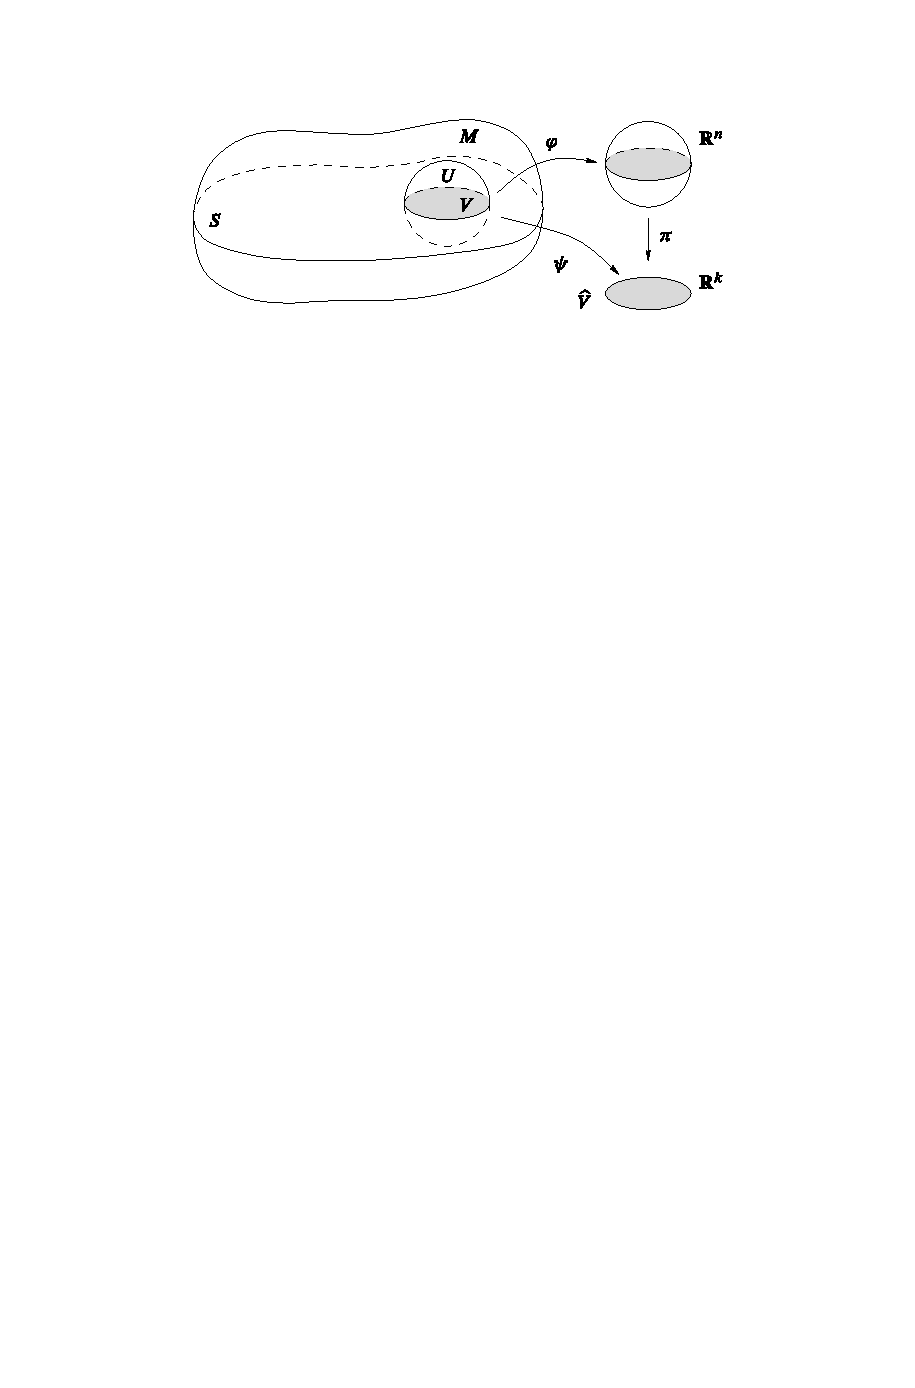
\includegraphics{pictures/slice-chart-1}
\caption{A chart for a subset satisfying the $k$-slice condition.}
\end{figure}\\
By definition of slice charts, $\varphi(V)$ is the intersection of $\varphi(U)$ with a certain $k$-slice $A\sub\R^n$ defined by setting $x^{k+1}=c^{k+1},\dots,x^n=c^n$, and therefore $\varphi(V)$ is open in $A$. Since $\pi|_A$ is a diffeomorphism from $A$ to $\R^k$, it follows that $\widehat{V}$ is open in $\R^k$. Moreover, is a homeomorphism because it has a continuous inverse $\varphi^{-1}\circ j|_{\widehat{V}}$, where
\[j:\R^k\to\R^n,\quad(x^1,\dots,x^k)\mapsto(x^1,\dots,x^k,c^{k+1},\dots,c^n)\]
Thus $S$ is a topological $k$-manifold, and the inclusion map $\iota:S\hookrightarrow M$ is a topological embedding.\par
To put a smooth structure on $S$, we need to verify that the charts constructed
above are smoothly compatible. Suppose $(U,\varphi)$ and $(U',\varphi')$ are two slice charts for $S$ in $M$ and let $(V,\psi)$, $(V',\psi')$ be the corresponding charts for $S$. The transition map is given by $\psi'\circ\psi^{-1}=\pi\circ\varphi'\circ\varphi^{-1}\circ j$, which is a composition of four smooth maps.
\begin{figure}[h]
\centering
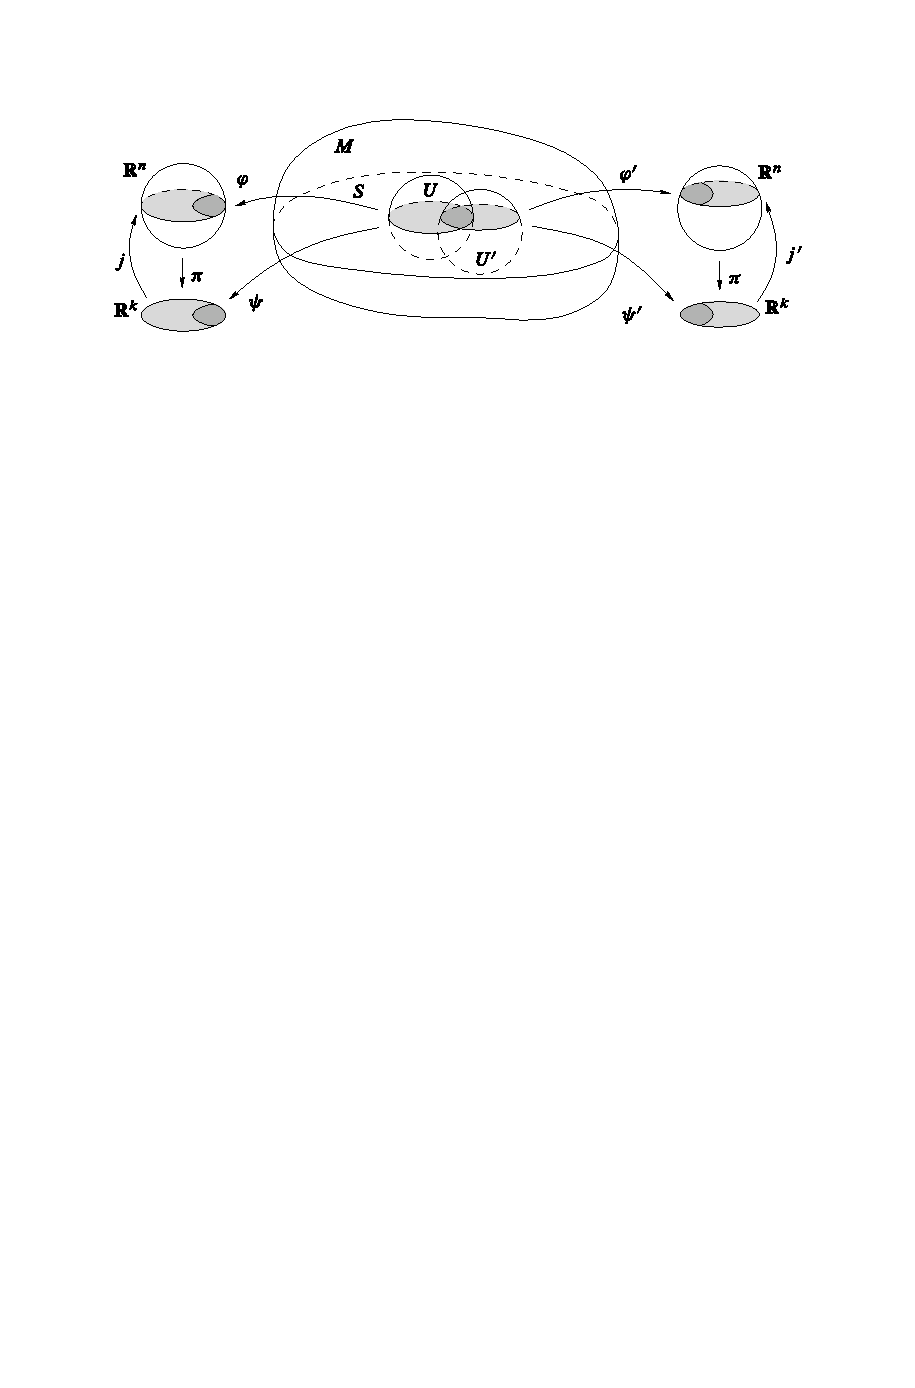
\includegraphics{pictures/slice-chart-2}
\caption{Smooth compatibility of slice charts.}
\end{figure}\\
Thus the atlas we have constructed is in fact a smooth atlas, and it defines a smooth structure on $S$. In terms of a slice chart $(U,\varphi)$ for $M$ and the corresponding chart $(V,\psi)$ for $S$, the inclusion map $S\hookrightarrow M$ has a coordinate representation of the form
\[(x^1,\dots,x^k)\mapsto(x^1,\dots,x^k,c^{k+1},\dots,c^n)\]
which is a smooth immersion. Since the inclusion is a smooth immersion and a topological embedding, $S$ is an embedded submanifold.
\end{proof}
If $M$ is a smooth manifold with nonempty boundary and $S\sub M$ is an embedded submanifold, then $S$ might intersect $\partial M$ in very complicated ways, so we will not attempt to prove any general results about the existence of slice charts for $S$ in $M$ in that case. However, in the special case in which the submanifold is the boundary of $M$ itself, the boundary charts for $M$ play the role of slice charts for $\partial M$ in $M$, and we do have the following result.
\begin{theorem}\label{boundary embedd mani}
If $M$ is a smooth $n$-manifold with boundary, then with the subspace topology, $\partial M$ is a topological $(n-1)$-dimensional manifold without boundary, and has a smooth structure such that it is a properly embedded submanifold of $M$.
\end{theorem}
\begin{proof}
With the subspace topology, $\partial M$ is closed in $M$. Let $\pi:\H^n\to\R^{n-1}$ be the projection on the first $n-1$ coordinates. For any boundary chart $(U,\varphi)$ of $M$, we define a new chart by
\[V=U\cap\partial M,\quad \widehat{V}=\pi\circ\varphi(V),\quad\psi=\pi\circ\varphi|_V\]
With these charts, $\partial M$ becoms a smooth manifold, and the inclusion map $\iota:\partial M\hookrightarrow M$ has coordinate representation 
\[(x^1,\dots,x^{n-1})\mapsto(x^1,\dots,x^{n-1},0)\]
Thus is a smooth immersion. Since $\partial M$ has the subspace topology, $\iota$ is also an embedding, thus a smooth embedding.
\end{proof}
\subsection{Level sets}
If $\varPhi:M\to N$ is any map and $c$ is any point of $N$, we call the set $\varPhi^{-1}(c)$ a \textbf{level set of $\bm{\varPhi}$}. In the special case $N=\R^k$ and $c=0$, the level set $\varPhi^{-1}(0)$ is usually called the \textbf{zero set of $\bm{\varPhi}$}.\par
It is easy to find level sets of smooth functions that are not smooth submanifolds.
For instance, consider the three smooth functions $\varTheta,\varPhi,\varPsi:\R^2\to\R$ defined by
\[\varTheta(x,y)=x^2-y,\quad \varPhi(x,y)=x^2-y^2,\quad \varPsi(x,y)=x^2-y^3\]
Although the zero set of $\varTheta$ is an embedded submanifold of $\R^2$ because it is the graph of the smooth function $f(x)=x^2$, neither the zero set of $\varPhi$ nor that of $\varPsi$ is an embedded submanifold. In fact, without further assumptions on the smooth function, the situation is about as bad as could be imagined: as Theorem~\ref{level set smooth functions} showed, every closed subset of $M$ can be expressed as the zero set of some smooth real-valued function.
\begin{theorem}[\textbf{Constant-Rank Level Set Theorem}]\label{constant rank level set}
Let $M$ and $N$ be smooth manifolds, and let $\varPhi:M\to N$ be a smooth map with constant rank $r$. Then each level set of $\varPhi$ is a properly embedded submanifold of codimension $r$ in $M$.
\end{theorem}
\begin{proof}
Write $m=\dim(M)$, $n=\dim(N)$, and $k=m-r$. Let $c\in N$ be arbitrary, and let $S$ denote the level set $\varPhi^{-1}(c)\sub M$. From the rank theorem, for each $p\in S$ there are smooth charts $(U,\varphi)$ centered at $p$ and $(V,\psi)$ centered at $c=\varPhi(p)$ in which $\varPhi$ has a coordinate representation of the form
\[\widehat{\varPhi}(x^1,\dots,x^r,x^{r+1},\dots,x^m)=(x^1,\dots,x^r,0,\dots,0)\]
and therefore
\[\varphi(S)\cap\varphi(U)=\widehat{\varPhi}^{-1}(0)=\{(x^1,\dots,x^r,x^{r+1},\dots,x^m)\in \varphi(U):x^1=\cdots=x^r=0\}\]
Thus $S$ satisfies the local $k$-slice condition, so it is an embedded submanifold of
dimension $k$. It is closed in $M$ by continuity, so it is properly embedded by Proposition~\ref{proper embedd iff}.
\end{proof}
\begin{corollary}[\textbf{Submersion Level Set Theorem}]\label{subm level set}
If $M$ and $N$ are smooth manifolds and $\varPhi:M\to N$ is a smooth submersion, then each level set of $\varPhi$ is a properly embedded submanifold whose codimension is equal to the dimension of $N$.
\end{corollary}
Corollary~\ref{subm level set} can be strengthened considerably, because we need only check the submersion condition on the level set we are interested in. If $\varPhi:M\to N$ is a smooth map, a point $p\in M$ is said to be a \textbf{regular point} of $d\varPhi_p:T_pM\to T_{\varPhi(p)}N$ is surjective; it is a \textbf{critical point} of $\varPhi$ otherwise. Note that the set of regular points of $\varPhi$ is always an open subset of $M$ by Proposition~\ref{local immersion subm}. A point $c\in N$ is said to be a \textbf{regular value} of $\varPhi$ if every point of the level set $\varPhi^{-1}(c)$ is a regular point, and a \textbf{critical value} otherwise. In particular, if $\varPhi^{-1}(c)=\emp$, then $c$ is a regular value. Finally, a level set $\varPhi^{-1}(c)$ is called a \textbf{regular level set} if $c$ is a regular value of $\varPhi$.
\begin{corollary}[\textbf{Regular Level Set Theorem}]\label{regular value level set}
Every regular level set of a smooth map between smooth manifolds is a properly embedded submanifold whose codimension is equal to the dimension of the codomain.
\end{corollary}
\begin{proof}
Let $\varPhi:M\to N$ be a smooth map and let $c\in N$ be a regular value. The set $U$ of points $p\in M$ where $\rank(d\varPhi_p)=\dim(N)$ is open in $M$ by Proposition~\ref{local immersion subm}, and contains $\varPhi^{-1}(c)$ because of the assumption that $c$ is a regular value. It follows that $\varPhi|_U:U\to N$ is a smooth submersion, and the preceding corollary shows that $\varPhi^{-1}(c)$ is an embedded submanifold of $U$. Since the composition of smooth embeddings $\varPhi^{-1}(c)\hookrightarrow U\hookrightarrow M$ is again a smooth embedding, it follows that $\varPhi^{-1}(c)$ is an embedded submanifold of $M$, and it is closed by continuity.
\end{proof}
\begin{remark}
Note that if we replace the submmersion condition in Corollary~\ref{regular value level set} by constant rank, then the claim is no longer true.
\end{remark}
\begin{proposition}\label{embedd mani iff level set}
Let $S$ be a subset of a smooth $m$-manifold $M$. Then $S$ is an embedded $k$-submanifold of $M$ if and only if every point of $S$ has a neighborhood $U$ in $M$ such that $U\cap S$ is a level set of a smooth submersion $\varPhi:U\to\R^{n-k}$.
\end{proposition}
\begin{proof}
First suppose $S$ is an embedded $k$-submanifold. If $(x^1,\dots,x^m)$ are slice coordinates for $S$ on an open subset $U\sub M$, the map $\varPhi:U\to\R^{m-k}$ given in coordinates by $(x^{k+1},\dots,x^m)$ is easily seen to be a smooth submersion, one of whose level sets is $S\cap U$. Conversely, suppose that around every point $p\in S$ there is a neighborhood $U$ and a smooth submersion $\varPhi:U\to\R^{m-k}$ such that $S\cap U$ is a level set of $\varPhi$. By the submersion level set theorem, $S\cap U$ is an embedded submanifold of $U$, so it satisfies the local slice condition, it follows that $S$ is itself an embedded submanifold of $M$.
\end{proof}
If $S\sub M$ is an embedded submanifold, a smooth map $\varPhi:M\to N$ such that $S$ is a regular level set of $\varPhi$ is called a \textbf{defining map} for $S$. In the special case $N=\R^{m-k}$, it is usually called a \textbf{defining function}. For example, $f(x)=|x|^2$ is a defining function for the sphere.\par More generally, if $U$ is an open subset of $M$ and $\varPhi:M\to N$ is a smooth
map such that $S\cap U$ is a regular level set of $\varPhi$, then $\varPhi$ is called a \textbf{local defining map} for $S$. Proposition~\ref{embedd mani iff level set} says that every embedded submanifold admits a local defining function in a neighborhood of each of its points.
\begin{example}[\textbf{Surfaces of Revolution}]\label{surfaces of revolution}
Let $H$ be the half-plane $\{(r,z):r>0\}$, and suppose $C\sub H$ is an embedded $1$-dimensional submanifold. The surface of revolution determined by $C$ is the subset $S_C\sub\R^3$ given by
\[S_C=\{(x,y,z):(\sqrt{x^2+y^2},z)\in C\}\]
The set $C$ is called its \textbf{generating curve}. If $\varphi:U\to\R$ is any local defining function for $C$ where $U\sub H$, we get a local defining function $\varPhi$ for $S_C$ by
\[\varPhi(x,y,z)=\varphi(\sqrt{x^2+y^2},z)\]
defined on the open subset
\[\widetilde{U}=\{(x,y,z):(\sqrt{x^2+y^2},z)\in U\}\sub\R^3\]
A computation shows that the Jacobian matrix of $\varPhi$ is
\[\partial\varPhi=\begin{bmatrix}
\dfrac{x}{r}\dfrac{\partial\varphi}{\partial r}(r,z)&\dfrac{y}{r}\dfrac{\partial\varphi}{\partial r}(r,z)&\dfrac{\partial\varphi}{\partial z}(r,z)
\end{bmatrix}\]
where we have written $r=\sqrt{x^2+y^2}$. At any point $(x,y,z)\in S_C$, at least one of the components of $\partial\varPhi(x,y,z)$ is nonzero, so $S_C$ is a regular level set of $\varPhi$ and is thus an embedded $2$-dimensional submanifold of $\R^3$.
\end{example}
\section{Immersed submanifolds}
Let $M$ be a smooth manifold with or without boundary. An \textbf{immersed submanifold} of $M$ is a subset $S\sub M$ endowed with a topology (not necessarily the subspace topology) with respect to which it is a topological manifold (without boundary), and a smooth structure with respect to which the inclusion map $S\hookrightarrow M$ is a smooth immersion. As for embedded submanifolds, we define the \textbf{codimension} of $S$ in $M$ to be $\dim(M)-\dim(S)$.\par
Immersed submanifolds often arise in the following way.
\begin{theorem}[\textbf{Images of Immersions as Submanifolds}]\label{image immersion submani}
Suppose $M$ is a smooth manifold with or without boundary, $N$ is a smooth manifold, and $F:N\to M$ is an injective smooth immersion. Let $S=F(N)$. Then $S$ has a unique topology and smooth structure such that it is a smooth submanifold of $M$ and such that $F:N\to S$ is a diffeomorphism onto its image.
\end{theorem}
\begin{proof}
The proof is very similar to that of Proposition~\ref{image of embedding}, except that now we also have to define the topology on $S$. We give $S$ a topology by declaring a set $U\sub S$ to be open if and only if $F^{-1}(U)\sub N$ is open, and then give it a smooth structure by taking the smooth charts to be those of the form $(F(U),\varphi\circ F^{-1})$, where $(U,\varphi)$ is any smooth chart for $N$. As in the proof of Proposition~\ref{image of embedding}, the smooth compatibility condition follows from that for $N$. With this topology and smooth structure on $S$, the map $F$ is a diffeomorphism onto its image, and these are the only topology and smooth structure on $S$ with this property. As in the embedding case, the inclusion $S\hookrightarrow M$ can be written as the composition
\[\begin{tikzcd}
S\ar[r,"F^{-1}"]&N\ar[r,"F"]&M
\end{tikzcd}\]
in this case, the first map is a diffeomorphism and the second is a smooth immersion, so the composition is a smooth immersion.
\end{proof}
The following observation is sometimes useful when thinking about the topology of an immersed submanifold.
\begin{proposition}\label{immersed submani topo}
Suppose $M$ is a smooth manifold and $S\sub M$ is an immersed submanifold. Then every subset of $S$ that is open in the subspace topology is also open in its given submanifold topology; and the converse is true if and only if $S$ is embedded.
\end{proposition}
\begin{proof}
Recall that a subset $U\sub S$ is open in the subspace topology if and only if there is an open subset $W$ of $M$ such that $U=W\cap S$. Let $\iota:S\hookrightarrow M$ be the inclusion, if $U=W\cap S$ is open in the subspace topology, then
\[\iota^{-1}(W)=W\cap S=U.\]
Since $\iota$ is continuous, this implies $U$ is open in the given submanifold topology of $S$.\par
Now the converse holds exactly when $\iota$ is an open map, thus if and only if $S$ is embedded.
\end{proof}
Given a smooth submanifold that is known only to be immersed, it is often useful
to have simple criteria that guarantee that it is embedded. The next proposition gives
several such criteria.
\begin{proposition}\label{immersed is embedd if}
Suppose $M$ is a smooth manifold with or without boundary, and $S\hookrightarrow M$ is an immersed submanifold. If any of the following holds, then $S$ is embedded.
\begin{itemize}
\item[(a)]$S$ has codimension $0$ in $M$.
\item[(b)]The inclusion map $S\sub M$ is proper.
\item[(c)]$S$ is compact.
\end{itemize}
\end{proposition}
\begin{proof}
For part (a), if $\dim(S)=\dim(M)$, then the inclusion map $\iota:S\hookrightarrow M$ is a local homeomorphism, hence open. This implies $\iota$ is an embedding. Part (b) and part (c) both imply that $\iota$ is closed, hence a embedding.
\end{proof}
Although many immersed submanifolds are not embedded, the next proposition
shows that the local structure of an immersed submanifold is the same as that of an embedded one.
\begin{figure}[h]
\centering
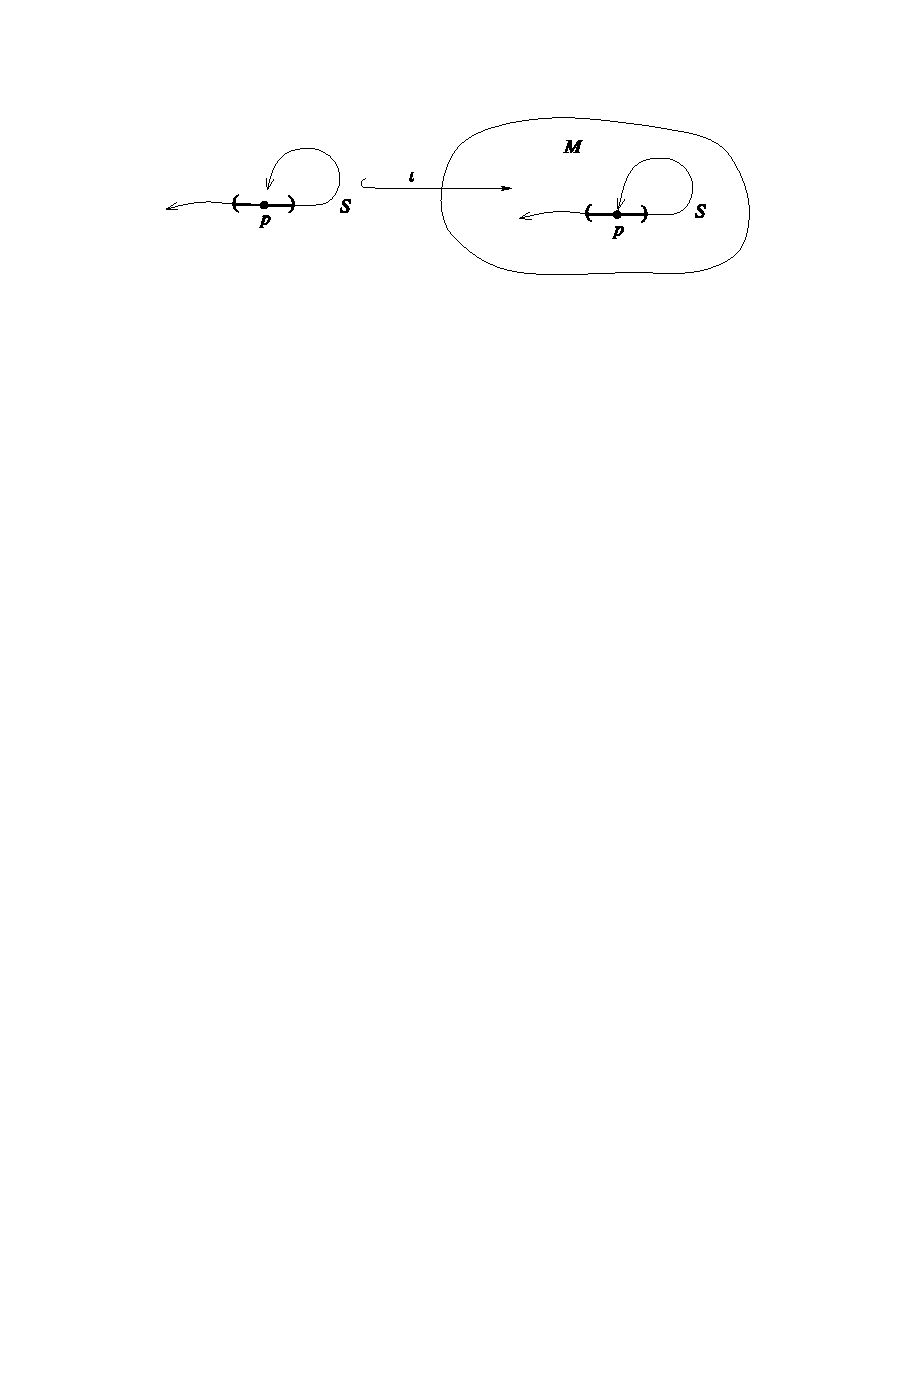
\includegraphics{pictures/immersered-mani}
\caption{An immersed submanifold is locally embedded.}
\end{figure}
\begin{theorem}[\textbf{Immersed Submanifolds Are Locally Embedded}]\label{immerse local embedd}
If $M$ is a smooth manifold with or without boundary, and $S\sub M$ is an immersed submanifold, then for each $p\in S$ there exists a neighborhood $U$ of $p$ in $S$ that is an embedded submanifold of $M$.
\end{theorem}
\begin{proof}
Theorem~\ref{immersion local embedding} shows that each $p\in S$ has a neighborhood $U$ in $S$ such that the inclusion $\iota|_U:U\hookrightarrow M$ is an embedding.
\end{proof}
It is important to be clear about what this proposition does and does not say: \textit{given an immersed submanifold $S\sub M$ and a point $p\in S$, it is possible to find a neighborhood $U$ of $p$ \textbf{in $\bm{S}$} such that $U$ is embedded; but it may not be possible to find a neighborhood $V$ of $p$ \textbf{in $\bm{M}$} such that $V\cap S$ is embedded}.\par
Suppose $S\sub M$ is an immersed $k$-dimensional submanifold. A \textbf{local parametrization} of $S$ is a continuous map $X:U\to M$ whose domain is an open subset $U\sub\R^k$, whose image is an open subset of $S$, and which, considered as a map into $S$, is a homeomorphism onto its image. It is called a \textbf{smooth local parametrization} if it is a diffeomorphism onto its image (with respect to $S$'s smooth manifold structure). If the image of $X$ is all of $S$, it is called a \textbf{global parametrization}.
\begin{proposition}
Suppose $M$ is a smooth manifold with or without boundary, $S\sub M$ is an immersed $k$-submanifold, $\iota:S\to M$ is the inclusion map, and $U$ is an open subset of $\R^k$. A map $X:U\to M$ is a smooth local parametrization of $S$ if and only if there is a smooth coordinate chart $(V,\varphi)$ for $S$ such that $X=\iota\circ\varphi^{-1}$. Therefore, every point of $S$ is in the image of some local parametrization.
\end{proposition}
\begin{proof}
Obviously each chart $(V,\varphi)$ defines a local parametrization $X=\iota\circ\varphi^{-1}$. Conversely, if $X=\iota\circ\varphi^{-1}$, then since $\varphi$ is a diffeomorphism, considered as a map from $V$ to $S$, $X$ is also a diffeomorphism.
\end{proof}
\begin{example}[\textbf{Graph Parametrizations}]
Suppose $U\sub\R^n$ is an open subset and $f:U\to\R^k$ is a smooth function. The map $\gamma_f:U\to\R^n\times\R^k$ given by $\gamma_f(u)=(u,f(u))$ is a smooth global parametrization of $\Gamma(f)$, called a \textbf{graph parametrization}.
\end{example}
\section{Restricting maps to submanifolds}
Given a smooth map $F:M\to N$, it is important to know whether $F$ is still smooth
when its domain or codomain is restricted to a submanifold. In the case of restricting the domain, the answer is easy.
\begin{theorem}[\textbf{Restricting the Domain of a Smooth Map}]\label{restrict domain}
If $M$ and $N$ are smooth manifolds with or without boundary, $F:M\to N$ is a smooth map, and $S\sub M$ is an immersed or embedded submanifold, then $F|_S:S\to N$ is smooth.
\end{theorem}
\begin{proof}
The inclusion map $\iota:S\hookrightarrow M$ is smooth by definition of an immersed submanifold. Since $F|_S=F\circ\iota$, the result follows.
\end{proof}
When the codomain is restricted, however, the resulting map may not be smooth,
as the following example shows.
\begin{example}
Let $S\sub\R^2$ be the figure-eight submanifold, with the topology and smooth structure induced by the immersion $\beta$ of Example~\ref{figure eight}. Define a smooth map $G:\R\to\R^2$ by
\[G(t)=(\sin 2t,\sin t)\]
It is easy to check that the image of $G$ lies in $S$. However, as a map from $\R$ to $S$, $G$ is not even continuous, because $\beta^{-1}\circ G$ is not continuous:
\[\begin{tikzpicture}[domain=0:4]
\draw[->] (-3,0) -- (3,0) node[right] {$x$};
\draw[->] (0,-2) -- (0,2) node[above] {$y$};
\draw (0,0)--(1,1);
\draw (0,0)--(-1,-1);
\draw (1,-1)--(2,0)--(3,1);
\draw (-1,1)--(-2,0)--(-3,-1);
\draw[dashed] (1,1)--(1,-1);
\draw[dashed] (-1,1)--(-1,-1);
\end{tikzpicture}\]
\end{example}
The next theorem gives sufficient conditions for a map to be smooth when its codomain is restricted to an immersed submanifold.It shows that the failure of continuity is the only thing that can go wrong.
\begin{theorem}[\textbf{Restricting the Codomain of a Smooth Map}]\label{restrict to codomain}
Suppose $M$ is a smooth manifold $($without boundary$)$, $S\sub M$ is an immersed submanifold, and $F:N\to M$ is a smooth map whose image is contained in $S$. If $F$ is continuous as a map from $N$ to $S$, then $F:N\to S$ is smooth.
\end{theorem}
\begin{figure}[h]
\centering
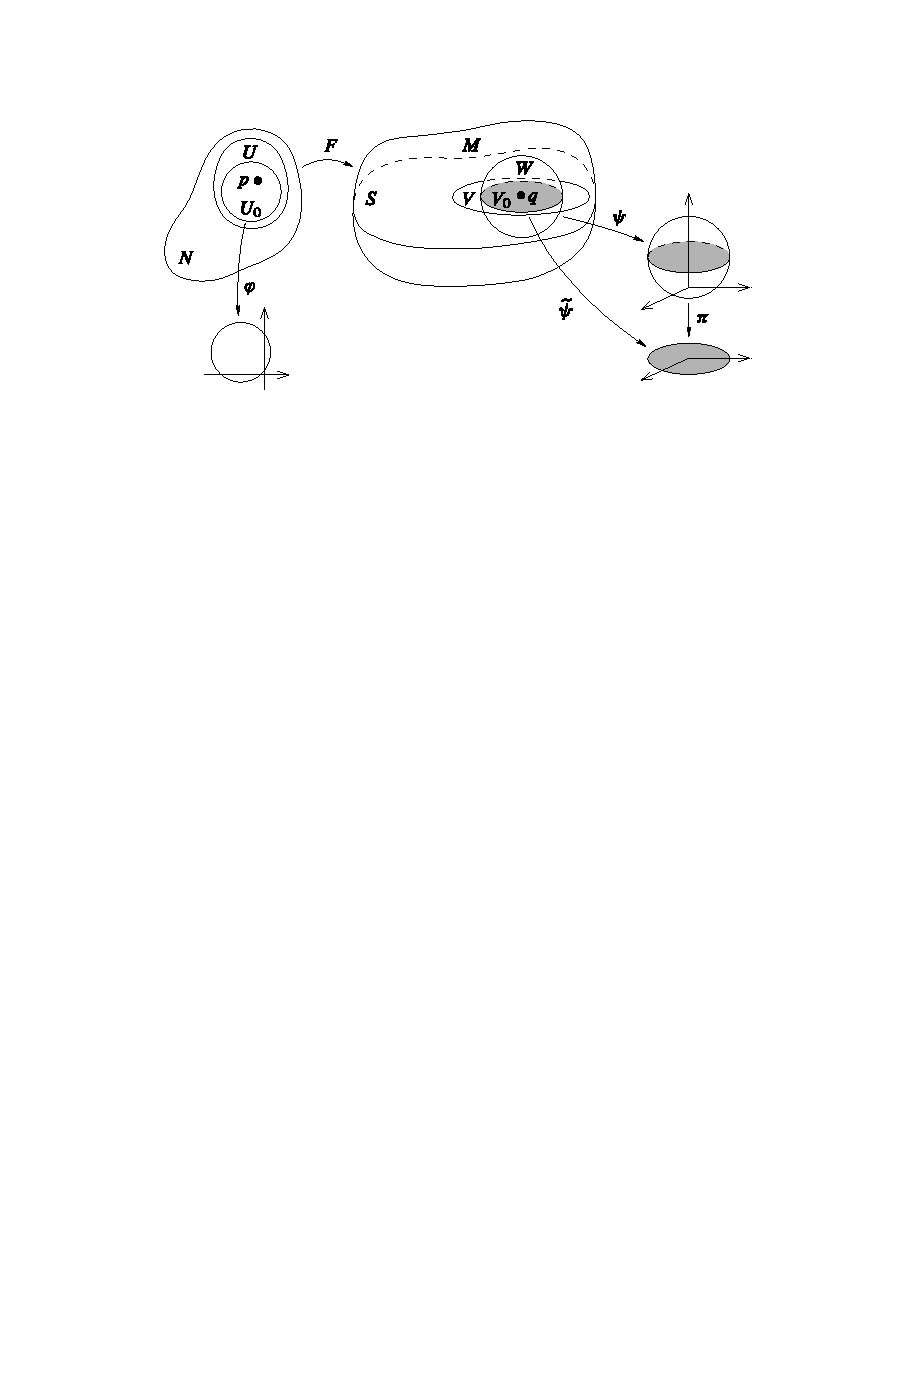
\includegraphics{pictures/restriction-codomain}
\caption{Proof of Theorem~\ref{restrict to codomain}.}
\end{figure}
\begin{proof}
Let $p\in N$ be arbitrary and let $q=F(p)\in S$. Proposition~\ref{immerse local embedd} guarantees that there is a neighborhood $V$ of $q$ in $S$ such that $\iota|_V:V\to M$ is a smooth embedding. Thus there exists a smooth chart $(W,\psi)$ for $M$ that is a slice chart for $V$ in $M$ centered at $q$. (\textit{It might not be a slice chart for $S$ in $M$.}) The fact that $(W,\psi)$ is a slice chart means that $(V_0,\tilde{\psi})$ is a smooth chart for $V$, where $V_0=W\cap V$ and $\tilde{\psi}=\pi\circ\psi$ with $\pi:\R^n\to\R^k$ the projection onto the first $k=\dim(S)$ coordinates. Since $V_0=(\iota|_V)^{-1}(W)$ is open in $V$, it is open in $S$ in its
given topology, and so $(V_0,\tilde{\psi})$ is also a smooth chart for $S$.\par
Let $U=F^{-1}(V_0)$, which is an open subset of $N$ containing $p$. (Here is where we use the hypothesis that $F$ is continuous into $S$.) Choose a smooth chart $(U_0,\varphi)$ for $N$ such that $p\in U_0\sub U$. Then the coordinate representation of $F:N\to S$ with respect to the charts $(U_0,\varphi)$ and $(V_0,\tilde{\psi})$ is
\[\tilde{\psi}\circ F\circ\varphi^{-1}=\pi\circ(\psi\circ F\circ\varphi^{-1})\]
which is smooth because $F:N\to M$ is smooth.
\end{proof}
In the special case in which the submanifold S is embedded, the continuity hypothesis is always satisfied.
\begin{corollary}\label{resrtict codomain to embedd}
Let $M$ be a smooth manifold and $S\sub M$ be an embedded submanifold. Then every smooth map $F:N\to M$ whose image is contained in $S$ is also smooth as a map from $N$ to $S$.
\end{corollary}
\begin{proof}
Since $S\sub M$ has the subspace topology, a continuous map $F:N\to M$ whose image is contained in $S$ is automatically continuous into $S$, by the characteristic
property of the subspace topology.
\end{proof}
If $M$ is a smooth manifold and $S\sub M$ is an immersed submanifold, then $S$ is said to be \textbf{weakly embedded} in $M$ if every smooth map $F:N\to M$ whose image lies in $S$ is smooth as a map from $N$ to $S$.
\subsection{Uniqueness of smooth structures on submanifolds}
Using the preceding results about restricting maps to submanifolds, we can prove the promised uniqueness theorem for the smoothmanifold structure on an embedded
submanifold.
\begin{theorem}\label{unique smooth embedd}
Suppose $M$ is a smooth manifold and $S\sub M$ is an embedded submanifold. The subspace topology on $S$ and the smooth structure described in Theorem~\ref{embedd submani iff local slice} are the only topology and smooth structure with respect to which $S$ is an embedded or immersed submanifold.
\end{theorem}
\begin{proof}
Suppose $S\sub M$ is an embedded $k$-dimensional submanifold. Theorem~\ref{embedd submani iff local slice} shows that it satisfies the local $k$-slice condition, so it is an embedded submanifold with the subspace topology and the smooth structure of Theorem~\ref{embedd submani iff local slice}. Suppose there were some other topology and smooth structure on $S$ making it into an immersed submanifold of some dimension. Let $\widetilde{S}$ denote the same set $S$, considered as a smooth manifold with the non-standard topology and smooth structure, and let $\tilde{\iota}:\widetilde{S}\hookrightarrow M$ denote the inclusion map, which by assumption is an injective immersion (but not necessarily an embedding). Because $\tilde{\iota}(\widetilde{S})=S$, Corollary~\ref{resrtict codomain to embedd} implies that $\tilde{\iota}$ is also smooth when considered as a map from $\widetilde{S}$ to $S$. For each $p\in\widetilde{S}$, the differential $d\tilde{\iota}_p:T_p\widetilde{S}\to T_pM$ is equal to the composition
\[\begin{tikzcd}
T_p\widetilde{S}\ar[r,"d\tilde{\iota}_p"]&T_pS\ar[r,"d\iota_p"]&T_pM
\end{tikzcd}\]
where $\iota:S\hookrightarrow M$ is also inclusion. Because this composition is injective (since $\widetilde{S}$ is assumed to be a smooth submanifold of $M$), $d\tilde{\iota}_p$ must be injective. In particular, this means that $\tilde{\iota}:\widetilde{S}\to S$ is an immersion. Because it is bijective, it follows from the global rank theorem that it is a diffeomorphism. In other words, the topology and smooth manifold structure of $\widetilde{S}$ are the same as those of $S$.
\end{proof}
Thanks to this uniqueness result, we now know that a subset $S\sub M$ is an embedded submanifold if and only if it satisfies the local slice condition, and if so, its
topology and smooth structure are uniquely determined. Because the local slice condition is a local condition, if every point $p\in S$ has a neighborhood $U\sub M$ such that $U\cap S$ is an embedded $k$-submanifold of $U$, then $S$ is an embedded $k$-submanifold of $M$.\par
The preceding theorem is false in general if $S$ is merely immersed; but we do have the following uniqueness theorem for the smooth structure of an immersed submanifold once the topology is known.
\begin{theorem}\label{unique struct immersed}
Suppose $M$ is a smooth manifold and $S\sub M$ is an immersed submanifold. For the given topology on $S$, there is only one smooth structure making $S$ into an immersed submanifold.
\end{theorem}
\begin{proof}
Let $\widetilde{S}$ denote the same set $S$, considered as a smooth manifold with the same topology and another smooth structure, and let $\tilde{\iota}:\widetilde{S}\hookrightarrow M$ denote the inclusion map, which by assumption is an injective immersion. Because $\tilde{\iota}(\widetilde{S})=S$ and the map $\tilde{\iota}:S\to\widetilde{S}$ is a homeomorphism since they have the same topology, Theorem~\ref{restrict to codomain} implies that $\tilde{\iota}$ is also smooth when considered as a map from $\widetilde{S}$ to $S$. Now the rest part is the same as that of Theorem~\ref{unique smooth embedd}.
\end{proof}
It is certainly possible for a given subset of $M$ to have more than one topology making it into an immersed submanifold. However, for weakly embedded submanifolds we have a stronger uniqueness result.
\begin{theorem}\label{unique smooth weak embedd}
If $M$ is a smooth manifold and $S\sub M$ is a weakly embedded submanifold, then $S$ has only one topology and smooth structure with respect to which it is an immersed submanifold.
\end{theorem}
\begin{proof}
This is immediate from the proof of Theorem~\ref{unique smooth embedd} and the definition of weakly embedded submanifold, applied on the inclusion $\tilde{\iota}:\widetilde{S}\to M$.
\end{proof}
\subsection{Extending functions from submanifolds}
Let $M$ be a smooth manifold with or without boundary, and let $S\sub M$ be a smooth submanifold. If $f:S\to\R$ is a function, there are two ways we might interpret the statement $f$ is smooth: it might mean that $f$ is smooth as a function on the smooth manifold $S$ (i.e., each coordinate representation is smooth), or it might mean that it is smooth as a function on the subset $S\sub M$ (i.e., it admits a smooth extension to a neighborhood of each point). We adopt the convention that the notation $f\in C^\infty(S)$ always means that $f$ is smooth in the former sense (as a function on the manifold $S$).
\begin{lemma}[\textbf{Extension Lemma}]\label{ext funct submani}
Let $M$ be a smooth manifold, $S\sub M$ be a smooth submanifold, and $f\in C^\infty(S)$.
\begin{itemize}
\item[(a)] $S$ is embedded if and only if every $f\in C^\infty(S)$ has a smooth extension to a neighborhood of $S$ in $M$.
\item[(b)] $S$ is properly embedded if and only if every $f\in C^\infty(S)$ has a smooth extension to all of $M$.
\end{itemize}
\end{lemma}
\begin{proof}
Let $k=\dim(S)$ and $\pi:\R^n\to\R^k$ be the projection. If $S$ is embedded, then each $p\in S$ is in the domain of a slice chart $(U_p,\varphi_p)$ in $M$ such that $f|_{S\cap U_p}=f(x^1,\dots,x^k)$ and the $x^i$ are slice coordinates. By replacing $U_p$ with $U_p\cap[(S\cap U_p)\times\R^{n-k}]$, we may assume that $\pi(U_p)\sub S\cap U_p$. Now we can extend $f|_{S\cap U_p}$ to $U_p$ by setting \[f_p(x^1,\dots,x^k,x^{k+1},\dots,x^n)=f|_{S\cap U_p}(x^1,\dots,x^n).\] 
The map $f_p:U_p\to\R$ is smooth because it is independent of its last $n-k$ coordinates and it is smooth with respect to its first $n$ coordinates.\par
The collection of open sets $U_p$ is an open cover of $S$, so let $(\psi_p)_{p\in S}$ be a partition of unity subordinate to this cover, and define $\widetilde{f}=\sum_{p\in S}\psi_pf_p$. If $x\in S$, then
\[\widetilde{f}(x)=\sum_{p\in S}\psi_p(x)f_p(x)=f(x)\]
Thus $\widetilde{f}$ is an extension of $f$.\par
Conversely, if any $f\in C^\infty(S)$ admits such an extension, let $U$ be an open subsetof $S$. For any $p\in U$, consider a function $f\in C^\infty(S)$ that is supported in $U$ and equal to $1$ at $p$. Let $\widetilde{f}:M\to\R$ be an extension of $f$, then the set $W=\{x\in M:\widetilde{f}(x)>0\}$ is open in $M$. Moreover, we have the following observation
\begin{itemize}
\item $p\in W$, since $\widetilde{f}(p)=f(p)=1$.
\item $W\cap S\sub U$, since $\widetilde{f}|_S=f$ and $\supp(f)\sub U$.
\end{itemize}
Thus $p$ has a neighborhood contained in $U$ with the subspace topology, which implies $U$ is open in the subspace topology. By Proposition~\ref{immersed submani topo}, this means $S$ is embedded. This completes the proof of (a).\par
Now we deal with part (b). One direction follows directly from Lemma~\ref{ext lem smooth func}, since if $S$ is properly embedded, then it is closed. Conversely, assume that each $f\in C^\infty(S)$ can be extended to $M$. By (a) we know that $S$ is embedded, so we only need to show $S$ is closed. If this is not the case, then there is some $p\in\widebar{S}-S$. We draw a contradition by constructing a function $f:M\to\R$ that only vanishes on $p$, and consider $1/f$: it is smooth on $S$, but can not be extended to $M$.\par
To do this, first take a smooth function $h:\R^n\to [0,1]$ with $h(0)=1$ and $h(x)<1$ for $x\neq 0$. For example 
\[h(x)=\begin{cases}
e^{-\frac{|x|^2}{1-|x|^2}}&|x|<1\\
0&\text{otherwise}
\end{cases}\]
Then choose a chart $(U,\varphi)$ of $M$ such that $\varphi(p)=0,\varphi(U)=\B^n$, and put 
\[f(q)=\begin{cases}
1-h(\varphi(q))&q\in U\\
1&q\notin U
\end{cases}\]
Now by the pasting lemma $f$ is smooth on all of $M$ and only vanishes in $p$.
\end{proof}
\section{The tangent space to a submanifold}
Let $M$ be a smooth manifold with or without boundary, and let $S\sub M$ be an immersed or embedded submanifold. Since the inclusion map $\iota:S\to M$ is a smooth
immersion, at each point $p\in S$ we have an injective linear map $d\iota_p:T_pS\to T_pM$. In terms of derivations, this injection works in the following way: for any vector $v\in T_pS$, the image vector $\widetilde{v}=d\iota_p(v)\in T_pM$ acts on smooth functions on $M$ by
\[\widetilde{v}(f)=d\iota_p(v)(f)=v(f\circ\iota)=v(f|_S)\]
We adopt the convention of identifying $T_pS$ with its image under this map, thereby
thinking of $T_pS$ as a certain linear subspace of $T_pM$.
\begin{proposition}\label{tangent submani}
Suppose $M$ is a smooth manifold with or without boundary, $S\sub M$ is an immersed or embedded submanifold, and $p\in S$. A vector $v\in T_pM$ is in $T_pS$ if and only if there is a smooth curve $\gamma:J\to M$ whose image is contained in $S$, and which is also smooth as a map into $S$, such that $0\in J$, $\gamma(0)=p$, and $\gamma'(0)=v$.
\end{proposition}
The next proposition gives a useful way to characterize $T_pS$ in the embedded case.
\begin{proposition}\label{tangent space submani}
Suppose $M$ is a smooth manifold, $S\sub M$ is an embedded submanifold, and $p\in S$. As a subspace of $T_pM$, the tangent space $T_pS$ is characterized by
\[T_pS=\{v\in T_pM:vf=0\text{ whenever }f\in C^\infty(M)\text{ and }f|_S=0\}\]
\end{proposition}
\begin{proof}
First suppose $v\in T_pS\sub T_pM$. This means, more precisely, that $v=d\iota_p(w)$ for some $w\in T_pS$, where $\iota:S\to M$ is inclusion. If $f$ is any smooth real-valued function on $M$ that vanishes on $S$, then $f\circ\iota\equiv 0$, so
\[vf=w(f\circ\iota)=0\]
Conversely, if $v\in T_pM$ satisfies $vf=0$ whenever $f$ vanishes on $S$, we need to
show that there is a vector $w\in T_pS$ such that $v=d\iota_p(w)$. Let $(x^1,\dots,x^n)$ be slice coordinates for $S$ in some neighborhood $U$ of $p$, so that $U\cap S$ is the subset of $U$ where $x^{k+1}=\cdots=x^n=0$, and $(x^1,\dots,x^k)$ are coordinates for $U\cap S$. Because the inclusion map $\iota:S\cap U\hookrightarrow M$ has the coordinate representation
\[\iota(x^1,\dots,x^k)=(x^1,\dots,x^k,0,\dots,0)\]
in these coordinates, it follows that $T_pS$ (that is, $d\iota_p(T_pS)$) is exactly the subspace of $T_pM$ spanned by $\partial/\partial x^1|_p,\dots,\partial/\partial x^k|_p$. If we write the coordinate representation
of $v$ as $v=v^i\frac{\partial}{\partial x^i}|_p$, we see that $v\in T_pS$ if and only if $v^i=0$ for $i>k$.\par
Let $\varphi$ be a smooth bump function supported in $U$ that is equal to $1$ in a neighborhood of $p$. Choose an index $j>k$, and consider the function $f(x)=\varphi(x)x^j$, extended to be zero on $M\setminus\supp(\varphi)$. Then $f$ vanishes identically on $S$, so
\[0=vf=\sum_{i=1}^{n}v^i\frac{\partial(\varphi(x)x^j)}{\partial x^i}(p)=v^j\]
Thus $v\in T_pS$.
\end{proof}
If an embedded submanifold is characterized by a defining map, the defining map gives a concise characterization of its tangent space at each point, as the next
proposition shows.
\begin{proposition}\label{tangent space level set}
Suppose $M$ is a smooth manifold and $S\sub M$ is an embedded submanifold. If $\varPhi:U\to N$ is any local defining map for $S$, then $T_pS=\ker d\varPhi_p$ for each $p\in S\cap U$.
\end{proposition}
\begin{proof}
Recall that we identify $T_pS$ with the subspace $d\iota_p:T_pS\to T_pM$, where $\iota:S\to M$ is the inclusion map. Because $\varPhi\circ\iota$ is constant on $S\cap U$, it follows that $d\varPhi_p\circ d\iota_p$ is the zero map from $T_pS$ to $T_{\varPhi(p)}N$, and therefore $\im d\iota_p\sub\ker d\varPhi_p$.\par
On the other hand, $d\varPhi_p$ is surjective by the definition of a defining map, so the rank-nullity law implies that
\[\dim(\ker d\varPhi_p)=\dim(T_pM)-\dim(T_{\varPhi(p)}N)=\dim(T_pS)=\dim(\im d\iota_p)\]
which implies $\im d\iota_p=\ker d\varPhi_p$.
\end{proof}
\begin{corollary}
Suppose $M$ and $N$ are smooth manifolds, $S\sub M$ is a level set of a smooth map $\varPhi:M\to N$ with constant rank. Then $T_pS=\ker d\varPhi_p$ for each $p\in S$.
\end{corollary}
\begin{proof}
Suppose $d\varPhi$ has rank $r$. Since $\varPhi\circ\iota$ is constant on $S$, we have $\im d\iota_p\sub\ker d\varPhi_p$. Also, 
\[\dim(\ker d\varPhi_p)=\dim(T_pM)-r=\dim(S)=\dim(\im d\iota_p)\]
Thus $\ker d\varPhi_p=\im d\iota_p=T_pS$.
\end{proof}
\begin{corollary}\label{tangent space constant rank}
Suppose $S\sub M$ is a level set of a smooth submersion $\varPhi=(\varPhi^1,\dots,\varPhi^k):M\to\R^k$. For any $p\in S$, a vector $v\in T_pM$ is tangent to $S$ if and only if $v\varPhi^1=\cdots=v\varPhi^k=0$.
\end{corollary}
\begin{proof}
We write $d\varPhi_p(v)=v^i\partial/\partial x^i|_{\varPhi(p)}\in T_{\varPhi(p)}\R^k$ and let $x^i$ be the $i$-th coordinate function, then
\[v^j=d\varPhi(v)(x^i)=v(x^i\circ\varPhi)=v\varPhi^i.\]
Thus $v\in\ker d\varPhi_p$ if and only if $v\varPhi^i=0$ for all $i=1,\dots,k$.
\end{proof}
\subsection{Tangent space to the boundary, inward-pointing and outward-pointing vectors}
If $M$ is a smooth manifold with boundary and $p\in\partial M$, it is intuitively evident that the vectors in $T_pM$ can be separated into three classes: those tangent to the boundary, those pointing inward, and those pointing outward. Formally, we make the following definition. If $p\in\partial M$, a vector $v\in T_pM-T_p\partial M$ is said to be \textbf{inward-pointing} if for some $\eps>0$ there exists a smooth curve $\gamma:[0,\eps)\to M$ such that $\gamma(0)=p$ and $\gamma'(0)=v$, and it is \textbf{outward-pointing} if there exists such a curve whose domain is $(-\eps,0]$. The following proposition gives another characterization of inward-pointing and outward-pointing vectors, which is usually much easier to check.
\begin{lemma}\label{inward pointing lem}
Let $M$ be a smooth manifold of dimensin $n$ with boundary, let $p$ be a boundary point, and let $v$ be a vector in $T_p(M)$. Let $(U,\varphi=(x^i))$ and $(V,\psi=(\widetilde{x}^j)$ be boundary charts at $p$, and in local coordinates, let
\[v=v^i\frac{\partial}{\partial x^i}\Big|_p,\quad v=\widetilde{v}^j\frac{\partial}{\partial\widetilde{x}^j}\Big|_p\]
Then either $v^n$ and $\widetilde{v}^n$ are both $0$, or they are both nonzero with the same sign.
\end{lemma}
\begin{proof}
We assume without loss of generality that $p$ is mapped to zero in both charts. Consider the transition function $\psi\circ\varphi^{-1}:\varphi(W)\to\psi(W)$ where $W=U\cap\widetilde{U}$:
\[\psi\circ\varphi^{-1}(x^1,\dots,x^n)=(\widetilde{x}^1,\dots,\widetilde{x}^n)\]
By the invariance boundary theorem, $\psi\circ\varphi^{-1}$ sends boundary (interior) points of $\H^n$ to boundary (interior) points of $\H^n$. Thus
\[\widetilde{x}^n(x^1,\dots,x^{n-1},0)=0\And\widetilde{x}^n(x^1,\dots,x^{n-1},x^n)>0\text{ \textit{if} } x^n>0.\]
It follows that
\[\frac{\partial\widetilde{x}^n}{\partial x^i}(p)=0\for 1\leq i\leq n-1\]
and
\begin{align*}
\frac{\partial\widetilde{x}^n}{\partial x^n}(p)=\lim_{r\to 0^+}\frac{\widetilde{x}^n(0,\dots,0,r)-\widetilde{x}^n(0,\dots,0,0)}{r-0}=\lim_{r\to 0^+}\frac{\widetilde{x}^n(0,\dots,0,r)}{r}\geq 0
\end{align*}
Also, the Jacobian matrix of $\psi\circ\varphi^{-1}$ has the form
\[\partial(\psi\circ\varphi^{-1})(p)=\begin{pmatrix}
\dfrac{\partial\widetilde{x}^j}{\partial x^i}&\dfrac{\partial\widetilde{x}^j}{\partial x^n}\\[8pt]
0&\dfrac{\partial\widetilde{x}^n}{\partial x^n}
\end{pmatrix}\]
Since $\psi\circ\varphi^{-1}$ is a diffeomorphism, we have $\partial\widetilde{x}^n/\partial x^n(p)>0$. Now from the formula $(\ref{coordinate change-1})$,
\[\widetilde{v}^n=v^i\frac{\partial\widetilde{x}^n}{\partial x^i}=v^n\frac{\partial\widetilde{x}^n}{\partial x^n}\]
The result now follows.
\end{proof}
\begin{proposition}\label{inward outward vector iff}
Suppose $M$ is a smooth $n$-dimensional manifold with boundary, $p\in\partial M$, and $(x^i)$ are any smooth boundary coordinates defined on a neighborhood of $p$. The inward-pointing vectors in $T_pM$ are precisely those with positive $x^n$-component, the outward-pointing ones are those with negative $x^n$-component, and the ones tangent to $\partial M$ are those with zero $x^n$-component. Thus, $T_pM$ is the disjoint union of $T_p\partial M$, the set of inward-pointing vectors, and the set of outward-pointing vectors, and $v\in T_pM$ is inward-pointing if and only if $-v$ is outwardpointing.
\end{proposition}
\begin{proof}
We assume without loss of generality that $p$ is mapped to zero. If $\gamma:[0,\eps)\to M$ is a sooth curve such that $\gamma(0)=p$ and $\gamma'(0)=v$. Then in this coordinate we have (since $\gamma^n(t)\geq 0$)
\[\dot{\gamma}^n(0)=\lim_{t\to 0^+}\frac{\gamma^n(t)-\gamma^n(0)}{t-0}=\lim_{t\to 0^+}\frac{\gamma^n(t)}{t}\geq 0\]
Now it follows from Lemma~\ref{inward pointing lem} that $v$ has positive $x^n$-component in any coordinate chart of $p$. The same result holds for outward-pointing vectors, with the observation
\[\dot{\gamma}^n(0)=\lim_{t\to 0^-}\frac{\gamma^n(t)-\gamma^n(0)}{t-0}=\lim_{t\to 0^+}\frac{\gamma^n(t)}{t}\geq 0\]
for any curve $\gamma:(-\eps,0]\to M$.\par
Now let $v=v^i\partial/\partial x^i$ with $x^n>0$, we construct a curve $\gamma:[0,\eps)\to M$ for suitable $\eps>0$ as 
\[\gamma(t)=(v^1t,\dots,v^nt)+\widehat{p}\]
where $\widehat{p}$ is the coordinate of $p$. Then $\gamma(0)=0$ and $\gamma'(0)=v$, and therefore $v$ is outward-pointing. The same can be done when $v^n<0$, with $\gamma$ being defined on $(-\eps,0]$.
\end{proof}
If $M$ is a smooth manifold with boundary, a \textbf{boundary defining function} for $M$ is a smooth function $f:M\to [0,+\infty)$ such that $f^{-1}(0)=\partial M$ and $df_p\neq0$ for all $p\in\partial M$. For example, $f(x)=1-|x|^2$ is a boundary defining function for the closed unit ball $\widebar{B}^n$.
\begin{proposition}\label{boundary defining function exist}
Every smooth manifold with boundary admits a boundary defining function.
\end{proposition}
\begin{proof}
Let $\{(U_\alpha,\varphi_\alpha)\}$ be a collection of smooth charts whose domains cover $M$. For each $\alpha$, define a smooth function $f_\alpha:U_\alpha\to[0,+\infty)$ as follows: if $U_\alpha$ is an interior chart, let $f_\alpha\equiv1$; while if $U_\alpha$ is a boundary chart, let $f_\alpha(x^1,\dots,x^{n})=x^n$ (the $n$-th coordinate function in that chart). Thus, $f_\alpha(p)$ is positive if $p\in\Int M$ and zero if $p\in\partial M$. Let $\{\psi_\alpha\}$ be a partition of unity subordinate to this cover, and let $f=\sum_\alpha f_\alpha\psi_\alpha$. Then $f$ is smooth, identically zero on $\partial M$, and strictly positive in $\Int M$. To see that $df$ does not vanish on $\partial M$, suppose $p\in\partial M$ and $v$ is an inward-pointing vector at $p$. For each $\alpha$ such that $p\in U_\alpha$, we have $f_\aleph(p)=0$ and $df_\alpha|_p(v)=dx^n|_p(v)>0$ by Proposition~\ref{inward outward vector iff}. Thus
\[df_p(v)=\sum_\alpha\big(f_\alpha(p)d\psi_\alpha|_p(v)+\psi_\alpha(p)df_\alpha|_p(v)\big).\]
For each $\alpha$, the first term in parentheses is zero and the second is nonnegative, and there is at least one $\alpha$ for which the second term is positive. Thus $df_p(v)>0$, which implies that $df_p\neq0$.
\end{proof}
\begin{proposition}\label{inward derivative crit}
Suppose $M$ is a smooth manifold with boundary, $f$ is a boundary defining function, and $p\in\partial M$. Then a vector $v\in T_pM$ is inward-pointing if and only if $vf>0$, outward-pointing if and only if $vf<0$, and tangent to $\partial M$ if and only if $vf=0$.
\end{proposition}
\begin{proof}
Let $\iota:\partial M\to M$ be the inclusion, and $p\in\partial M$ be any point. Since $f$ is constant on $\partial M$, $df_p\circ d\iota_p$ is zero on $\partial M$, hence $T_p\partial M\sub\ker df_p$. Moreover, since $df_p\neq 0$ on $p\in\partial M$, we have
\[\dim(\ker df_p)=\dim(M)-1=\dim(T_p\partial M)\]
Thus $T_p\partial M=\ker df_p$. For each point $p$, there is a boundary chart $(U,\varphi)$ in $M$ such that 
\[f(x^1,\dots,x^n)=x^n\]
If we write $df_p(v)=v^i\partial/\partial x^i|_{f(p)}$, then $vf=v^n$. Thus the claim follows from Proposition~\ref{inward outward vector iff}.
\end{proof}
\begin{example}
Consider the subset $S=\{(x,y)\in\R^2:y=|x|\}$. It is easy to check that $S-\{(0,0)\}$ is an embedded $1$-dimensional submanifold of $\R^2$, so if $S$ itself is a smooth submanifold at all, it must be $1$-dimensional. Suppose there were some smooth manifold structure on $S$ making it into an immersed submanifold. Then $T_{(0,0)}S$ would be a $1$-dimensional subspace of $T_{(0,0)}\R^2$, so by Proposition~\ref{tangent submani} there is a curve $\gamma:(-\eps,\eps)\to\R^2$ whose image lies in $S$, and that satisfies $\gamma(0)=(0,0)$ and $\gamma'(0)\neq0$. Writing $\gamma(t)=(x(t),y(t))$, we see that $y(t)$ takes a global minimum at $t=0$, so $y'(0)=0$. On the other hand, because every point $(x,y)\in S$ satisfies $x^2=y^2$, we have $x^2(t)=y^2(t)$ for all $t$. Differentiating twice and setting $t=0$, we conclude that $x'(0)=y'(0)=0$, which is a contradiction. Thus, there is no such smooth manifold structure.
\end{example}
\section{Submanifolds with boundary}
If $M$ is a smooth manifold with or without boundary, a \textbf{smooth submanifold with boundary} in $M$ is a subset $S\sub M$ endowed with a topology and smooth structure making it into a smooth manifold with boundary such that the inclusion map is a smooth immersion. If the inclusion map is an embedding, then it is called an \textbf{embedded submanifold with boundary}; in the general case, it is an \textbf{immersed submanifold with boundary}. The terms \textbf{codimension} and \textbf{properly embedded} are defined just as in the submanifold case.\par
One particular type of submanifold with boundary is especially important. If $M$
is a smoothmanifold with or without boundary, a \textbf{regular domain} in $M$ is a properly embedded codimension-$0$ submanifold with boundary. Familiar examples are the closed upper half space $\H^n\sub\R^n$, the closed unit ball $\widebar{B}^n\sub\R^n$, and the closed upper hemisphere in $S^n$.
\begin{proposition}
Suppose $M$ is a smooth manifold without boundary and $D\sub M$ is a regular domain. The topological interior and boundary of $D$ are equal to its manifold interior and boundary, respectively.
\end{proposition}
\begin{proof}
Let $F:D\hookrightarrow M$ denote the inclusion map. Suppose $p\in D$ is arbitrary. If $p$ is in the manifold boundary of $D$, Theorem~\ref{rank thm manifold boundary} shows that there exist a smooth boundary chart $(U,\varphi)$ for $D$ centered at $p$ and a smooth chart $(V,\psi)$ for $M$ centered at $p$ in which $F$ has the coordinate representation $F(x^1,\dots,x^n)=(x^1,\dots,x^n)$, where $n=\dim(M)=\dim(D)$. Since $D$ has the subspace topology, $U=D\cap W$ for some open subset $W\sub M$, so $V_0:=V\cap W$ is a neighborhood of $p$ in $M$ such that $V_0\cap D$ consists of all the points in $V_0$ whose $x^n$ coordinate is nonnegative. Thus every neighborhood of $p$ intersects both $D$ and $M-D$, so $p$ is in the topological boundary of $D$.\par
On the other hand, suppose $p$ is in the manifold interior of $D$. The manifold
interior is a smooth embedded codimension-$0$ submanifold without boundary in $M$,
so it is an open subset by Proposition~\ref{open submani iff}. Thus $p$ is in the topological interior of $D$.\par 
Conversely, if $p$ is in the topological interior of $D$, then it is not in the topological boundary, so the preceding argument shows that it is not in the manifold boundary and hence must be in the manifold interior. Similarly, if $p$ is in the topological boundary, it is also in the manifold boundary.
\end{proof}
Here are some ways in which regular domains often arise.
\begin{proposition}\label{regular domain}
Suppose $M$ is a smooth manifold and $f\in C^\infty(M)$.
\begin{itemize}
\item[(a)]For each regular value $b$ of $f$, the set $f^{-1}((-\infty,b])$ is a regular domain in $M$.
\item[(b)]If $a$ and $b$ are two regular values of $f$ with $a<b$, then $f^{-1}([a,b])$ is a regular domain in $M$.
\end{itemize}
\begin{proof}
We only deal with part (a), part (b) can be done in the same manner. Since $f$ is continuous, $f^{-1}((-\infty,b))$ is open in $M$ and $f^{-1}((-\infty,b])$ is closed in $M$, hence we only need to show thw existence of boundary charts.\par 
Let $p\in M$ be in the level set $f^{-1}(b)$, then since $b$ is a regular value, there is a chart $(U,\varphi)$ in $M$ containing $p$ such that
\[\widehat{f}=f\circ\varphi^{-1}(x^1,\dots,x^n)=b-x_n,\]
and therefore $\widehat{f}^{-1}((-\infty,b])=U\cap\H^n$. Set $\widetilde{U}=U\cap \H^n$, we get a boundary chart $(\widetilde{U},\varphi)$ for $p$. 
\end{proof}
\end{proposition}
A set of the form $f^{-1}((-\infty,b])$ for $b$ a regular value of $f$ is called a \textbf{regular sublevel set} of $f$. Part (a) of the preceding theorem shows that every regular sublevel set of a smooth real-valued function is a regular domain. If $D\sub M$ is a regular domain and $f\in C^\infty(M)$ is a smooth function such that $D$ is a regular sublevel set of $f$, then $f$ is called a \textbf{defining function} for $D$.
\begin{theorem}
If $M$ is a smooth manifold and $D\sub M$ is a regular domain, then there exists a defining function for $D$. If $D$ is compact, then $f$ can be taken to be a smooth exhaustion function for $M$.
\end{theorem}
\begin{proposition}[\textbf{Properties of Submanifolds with Boundary}]
Suppose $M$ is a smooth manifold with or without boundary.
\begin{itemize}
\item[(a)]Every open subset of $M$ is an embedded codimension-$0$ submanifold with $($possibly empty$)$ boundary.
\item[(a)]If $N$ is a smooth manifold with boundary and $F:N\to M$ is a smooth embedding, then with the subspace topology $F(N)$ is a topological manifold with boundary, and it has a smooth structure making it into an embedded submanifold
with boundary in $M$.
\item[(c)]An embedded submanifold with boundary in $M$ is properly embedded if and
only if it is closed.
\item[(d)]If $S\sub M$ is an immersed submanifold with boundary, then for each $p\in S$ there exists a neighborhood $U$ of $p$ in $S$ that is embedded in $M$.
\end{itemize}
\end{proposition}
In order to adapt the results that depended on the existence of local slice charts,
we have to generalize the local $k$-slice condition as follows. Suppose $M$ is a smooth manifold (without boundary). If $(U,(x^i))$ is a chart for $M$, a \textbf{$\bm{k}$-dimensional half-slice} of $U$ is a subset of the following form for some constants $c^{k+1},\dots,c^n$:
\[\{(x^1,\dots,x^n)\in U:x^{k+1}=c^{k+1},\dots,x^n=c^n,\text{ and }x^k\geq 0\}\]
We say that a subset $S\sub M$ satisfies the \textbf{local $\bm{k}$-slice condition for submanifolds with boundary} if each point of $S$ is contained in the domain of a smooth chart $(U,(x^i))$ such that $S\cap U$ is either an ordinary $k$-dimensional slice or a $k$-dimensional half-slice. In the former case, the chart is called an \textbf{interior slice chart} for $S$ in $M$, and in the latter, it is a \textbf{boundary slice chart} for $S$ in $M$.
\begin{proposition}
Let $M$ be a smooth $n$-manifold without boundary. If $S\sub M$ is an embedded $k$-dimensional submanifold with boundary, then $S$ satisfies the local $k$-slice condition for submanifolds with boundary. Conversely, if $S\sub M$ is a subset
that satisfies the local $k$-slice condition for submanifolds with boundary, then with the subspace topology, $S$ is a topological $k$-manifold with boundary, and it has a smooth structure making it into an embedded submanifold with boundary in $M$.
\end{proposition}
Using the preceding theorem, one can readily prove the following theorem.
\begin{theorem}[\textbf{Restricting Maps to Submanifolds with Boundary}]
Suppose $M$ and $N$ are smooth manifolds with boundary and $S\sub M$ is an embedded submanifold with boundary.
\begin{itemize}
\item[(a)]Restricting the domain: If $F:M\to N$ is a smooth map, then $F|_S:S\to N$ is smooth.
\item[(b)]Restricting the codomain: If $\partial M=\emp$ and $F:N\to M$ is a smooth map whose image is contained in $S$, then $F$ is smooth as a map from $N$ to $S$.
\end{itemize}
\end{theorem}
\section{Exercise}
\begin{exercise}
Consider the map $\varPhi:\R^4\to\R^2$ defined by
\[\varPhi(x,y,s,t)=(x^2+y,x^2+y^2+s^2+t^2+y)\]
Show that $(0,1)$ is a regular value of $\varPhi$, and that the level set $\varPhi^{-1}(0,1)$ is diffeomorphic to $S^2$.
\end{exercise}
\begin{proof}
We have
\[\partial\varPhi=\begin{bmatrix}
2x&1&0&0\\
2x&2y+1&2s&2t
\end{bmatrix},\quad\varPhi^{-1}(0,1)=\left\{\begin{array}{l}
x^2+y=0\\
x^2+y^2+s^2+t^2+y=1
\end{array}\right. =\left\{\begin{array}{l}
y=-x^2\\
x^4+s^2+t^2=1
\end{array}\right. \]
Thus $(0,1)$ is a regular value. Obviously the set $S=\{x^4+s^2+t^2=1\}$ is diffeomorphic to $S^2$. Since $\varPhi^{-1}(0,1)$ can be viewed as the graph of $S$, the claim follows.
\end{proof}
\begin{exercise}
Suppose $M\sub\R^n$ is an embedded m-dimensional submanifold, and let $UM\sub T\R^n$ be the set of all unit tangent vectors to $M$:
\[UM=\{(x,v)\in T\R^n:x\in M,v\in T_xM,|v|=1\}\]
It is called the \textbf{unit tangent bundle} of $M$. Prove that $UM$ is an embedded $(2m-1)$-dimensional submanifold of $T\R^n\approx\R^n\times\R^n$.
\end{exercise}
\begin{proof}
Consider the smooth map $F:TM\to\R$ defined by
\[(x,v)\mapsto|v|^2\]
Then $1$ is a regular value of $F$, and we have
\[UM=F^{-1}(1)\]
Thus $UM$ is an embedded $(2m-1)$-dimensional submanifold.
\end{proof}
\begin{exercise}\label{delete coordinate ball}
Suppose $M$ is a smooth $n$-manifold and $B\sub M$ is a regular coordinate ball. Show that $M-B$ is a smooth manifold with boundary, whose boundary is diffeomorphic to $S^{n-1}$.
\end{exercise}
\begin{proof}
We assume without loss of genrality that $M=\R^n$. To define the boundary chart, we consider the following map:
\[\pi:(x^1,\dots,x^{n-1},x^n)\mapsto(x^1,\dots,x^{n-1},|x|-1)\]
\end{proof}
\begin{exercise}
Let $S\sub\R^2$ be the boundary of the square of side $2$ centered at the origin. Show that $S$ does not have a topology and smooth structure in which it is an immersed submanifold of $\R^2$.
\end{exercise}
\begin{proof}
The set $S$ is given by
\[S=\{(x,y)\in\R^2:\max\{|x|,|y|\}\leq 1\}\]
Now assmue the converse, then $T_{(1,1)}S$ is a one-dimensional subspace, hence by Proposition~\ref{tangent space submani} there is a smooth curve $\gamma:(-\eps,\eps)\to \R^2$ whose image lies in $S$, and that satisfies $\gamma(0)=(1,1)$ and $\gamma'(0)\neq 0$. Write $\gamma(t)=(x(t),y(t))$, then $x(t)$ and $y(t)$ both take an extreme at $t=0$, hence $x'(t)=y'(t)=0$. This is a contradiction.
\end{proof}
\begin{exercise}
Suppose $E$ and $M$ are smooth manifolds with boundary, and $\pi:E\to M$ is a smooth covering map. Show that the restriction of $\pi$ to each connected component of $\partial E$ is a smooth covering map onto a component of $\partial M$.
\end{exercise}
\begin{proof}
Since $\partial E$ is properly embedded, we can restric the domain and codomains.
\end{proof}
\begin{exercise}
Prove that the image of the dense curve on the torus described in Example~\ref{dense curve torus} is a weakly embedded submanifold of $T^2$.
\end{exercise}
\begin{proof}
Let $S$ be the curve and $\gamma(t)=(e^{2\pi it},e^{2\pi i\alpha t})$ be the parametrization, $f:M\to T^2$ be a smooth map. We only need to check $f$ is continuous as a map from $M$ to $S$. Since the sets of the form $\gamma(t_0-\eps,t_0+\eps)$ for $t_0\in\R$ and $0<\eps<2\pi$ form a basis for the topology of $S$, to prove the continuity of $f$ it suffices to show that the inverse images of these sets under $f$ are open in $M$.\par
Given $t_0\in\R$ and $0<\eps<2\pi$, let $U$ denote the open set of $T^2$ given by the formula
\[U=\{(e^{2\pi it},e^{2\pi is}):-\eps<t<\eps,s\in\R\}\]
Let $\varphi:U\to(-\eps,\eps)\times S^1$ denote the homeomorphism 
\[\varphi(e^{2\pi it},e^{2\pi is})=(t,e^{2\pi i(s-\alpha t)})\]
Now we have
\[U\cap S=\{(e^{2\pi it},e^{2\pi i\alpha(t+n)}):-\eps<t<\eps,n\in\N\},\quad \varphi(U\cap S)=\bigcup_{n\in\N}(-\eps,\eps)\times\{e^{2\pi in\alpha}\}\]
It is easy to check that this equation represents the partition of $\varphi(U\cap S)$ into its path components. It follows that the path components of $U\cap S$ are
\[\varphi^{-1}((-\eps,\eps)\times\{e^{2\pi in\alpha}\})=\gamma(2\pi n-\eps,2\pi n+\eps),\quad\forall n\in\N\]
In particular, $\gamma(-\eps,\eps)$ is a path component of $U\cap S$. Now let $p\in f^{-1}(\gamma(-\eps,\eps))$ and $U$ be the path component of $M$ containting $p$. Then since $f(U)$ is path connected, it is contained in $\gamma(-\eps,\eps)$, which implies $U\sub f^{-1}(\gamma(-\eps,\eps))$. Thus $f^{-1}(\gamma(-\eps,\eps))$ is a union of some subcollection of path components of $f^{-1}(U)$, and is therefore open in $M$.
\end{proof}
\begin{exercise}
Show by example that an immersed submanifold $S\sub M$ might have more than one topology and smooth structure with respect to which it is an immersed submanifold.
\end{exercise}
\begin{proof}
Consider the figure-eight: give the parametrizations
\[F(t)=(\sin 2t,\sin t),\quad G(t)=(-\sin 2t,\sin t)\]
where $t\in(-\pi,\pi)$. Then 
\[G^{-1}\circ F(x)=\begin{cases}
\pi-x&x\in(0,\pi)\\
-\pi-x&x\in(-\pi,0)
\end{cases}\]
Thus the topology and smooth structure of these two parametrization are different.
\end{proof}
\begin{exercise}
Suppose $S\sub M$ is an embedded submanifold and $\gamma:J\to M$ is a smooth curve whose image happens to lie in $S$. Show that $\gamma'(t)$ is in the subspace $T_{\gamma(t)}S$ of $T_{\gamma(t)}M$ for all $t\in J$. Give a counterexample if $S$ is not embedded.
\end{exercise}
\begin{proof}
The figure-eight $S$ is an example, where $\gamma(t)=(-\sin 2t,\sin t)$. The vector $\gamma'(0)=(-1,1)$ is not in $T_0S=(t,t)$.
\end{proof}
\begin{exercise}
Suppose $M$ is a smooth manifold with boundary, $N$ is a smooth manifold, and $F:M\to N$ is a smooth map. Let $S=F^{-1}(c)$, where $c\in N$ is a regular value for both $F$ and $F|_{\partial M}$. Prove that $S$ is a smooth submanifold with boundary in $M$, with $\partial S=S\cap\partial M$.
\end{exercise}
\begin{proof}
The proof is similar to Proposition~\ref{constant rank level set}.
\end{proof}
\begin{exercise}
Suppose $M$ is a smooth manifold with boundary, $N$ is a smooth manifold, and $F:N\to M$ is a smooth map whose image is contained in $\partial M$. Show that $F$ is smooth as a map into $\partial M$, and use this to prove that $\partial M$ has a unique smooth structure making it an embedded submanifold of $M$.
\end{exercise}
\chapter{Sard's theorem}
\section{Sets of measure zero}
Recall what it means for a set $A\sub\R^n$ to have measure zero: for any $\delta>0$, $A$ can be covered by a countable collection of open rectangles, the sum of whose volumes is less than $\delta$.
\begin{lemma}\label{measure zero lem}
Suppose $A\sub\R^n$ is a compact subset whose intersection with $\{c\}\times\R^{n-1}$ has $(n-1)$-dimensional measure zero for every $c\in\R$. Then $A$ has $n$-dimensional measure zero.
\end{lemma}
\begin{proof}
This follows from Fubini's theorem.
\end{proof}
The most important sets of measure zero are graphs of continuous functions.
\begin{proposition}\label{graph measure zero}
Suppose $A$ is an open or closed subset of $\R^{n-1}$ or $\H^{n-1}$, and $f:A\to\R$ is a continuous function. Then the graph of $f$ has measure zero in $\R^n$.
\end{proposition}
\begin{proof}
First assume $A$ is compact. We prove the theorem in this case by induction on $n$. When $n=1$, it is trivial because the graph of $f$ is at most a single point. To prove the inductive step, we appeal to Lemma~\ref{measure zero lem}. For each $c\in\R$, the intersection of the graph of $f$ with $\{c\}\times\R^{n-1}$ is just the graph of the restriction of $f$ to $\{x\in A:x^1=c\}$, which is in turn the graph of a continuous function of $n-2$ variables. It follows by induction that each such graph has $(n-1)$-dimensional measure zero, and thus by Lemma~\ref{measure zero lem}, the graph of f itself has $n$-dimensional measure zero.\par
If $A$ is noncompact, it is a countable union of compact subsets, so the graph of $f$ is a countable union of sets of measure zero.
\end{proof}
\begin{proposition}
Every proper affine subspace of $\R^n$ has measure zero in $\R^n$.
\end{proposition}
\begin{proof}
Let $S\sub\R^n$ be a proper affine subspace. Suppose first that $\dim(S)=n-1$. Then there is at least one coordinate axis, say the $x^i$-axis, that is not parallel to $S$, and in that case $S$ is the graph of an affine function of the form $x^i=F(x^1,\dots,x{i-1},x^{i+1},\dots,x^n)$ so it has measure zero by Proposition~\ref{graph measure zero}. If $\dim(S)<n-1$, then $S$ is contained in some affine subspace of dimension $n-1$, so $S$ has measure zero.
\end{proof}
Our goal is to extend the notion of measure zero in a diffeomorphism-invariant fashion to subsets of manifolds. Because a manifold does not come with a metric, volumes of cubes or balls do not make sense, so we cannot simply use the same definition. However, the key is provided by the next proposition, which implies that
the condition of having measure zero is diffeomorphism-invariant for subsets of $\R^n$.
\begin{proposition}\label{image measure zero}
Suppose $A\sub\R^n$ has measure zero and $F:A\to\R^n$ is a smooth map. Then $F(A)$ has measure zero.
\end{proposition}
\begin{proof}
By definition, for each $p\in A$, $F$ has an extension to a smooth map, which we still denote by $F$, on a neighborhood of $p$ in $\R^n$. Shrinking this neighborhood
if necessary, we may assume that there is an open ball $U$ containing $p$ such that $F$ extends smoothly to $\widebar{U}$. Now $A$ is covered by countably many such precompact open subsets, so $F(A)$ is the union of countably many sets of the form $F(A\cap\widebar{U})$. Thus, it suffices to show that each such set has measure zero.\par
Since $\widebar{U}$ is compact, there is a constant $C$ such that $|\partial F(x)|\leq C$ for all $x\in\widebar{U}$. Using the Lipschitz estimate for smooth functions, we have
\begin{align}\label{image measure zero-1}
|F(x)-F(x')|\leq C|x-x'|
\end{align}
for all $x,x'\in\widebar{U}$.\par
Given $\delta>0$, choose a countable cover $\{B_j\}$ of $A\cap\widebar{U}$ by open balls satisfying $\sum_j\vol(B_j)<\delta$. Then by $(\ref{image measure zero-1})$, $F(\widebar{U}\cap B_j)$ is contained in a ball $\widetilde{B}_j$ whose radius is no more than $C$ times that of $B_j$. We conclude that $F(A\cap\widebar{U})$ is contained in the collection of balls $\{\widetilde{B}_j\}$, the sum of whose volumes is at most $C^n\delta$. Since this can be made as small as desired, it follows that $F(A\cap\widebar{U})$ has measure zero.
\end{proof}
If $M$ is a smooth $n$-manifold with or without boundary, we say that a subset $A\sub M$ has measure zero in $M$ if for every smooth chart $(U,\varphi)$ for $M$, the subset $\varphi(U)\sub\R^n$ has $n$-dimensional measure zero. The following lemma shows that we need only check this condition for a single collection of smooth charts whose domains cover $A$.
\begin{lemma}
Let $M$ be a smooth $n$-manifold with or without boundary and $A\sub M$. Suppose that for some collection $\{(U_\alpha,\varphi_\alpha)\}$ of smooth charts whose domains cover $A$ and $\varphi_\alpha(A\cap U_\alpha)$ has measure zero in $\R^n$ for each  $\alpha$. Then $A$ has measure zero in $M$.
\end{lemma}
\begin{proof}
Let $(V,\psi)$ be an arbitrary smooth chart. We need to show that $\psi(A\cap V)$ has measure zero. Some countable collection of the $U_\alpha$'s covers $A\cap V$. For each such $U_\alpha$, we have
\[\psi(A\cap V\cap U_\alpha)=(\psi\circ\varphi_\alpha^{-1})\circ\varphi_\alpha(A\cap V\cap U_\alpha)\]
Now, $\varphi_\alpha(A\cap V\cap U_\alpha)$ is a subset of $\varphi_\alpha(A\cap U_\alpha)$, which has measure zero in $\R^n$ by hypothesis. By Proposition~\ref{image measure zero} applied to $\psi\circ\varphi_\alpha^{-1}$, therefore, $\psi(A\cap V\cap U_\alpha)$ has measure zero. Since $\psi(A\cap V)$ is the union of countably many such sets, it too has measure zero.
\end{proof}
\begin{proposition}
Suppose $M$ is a smooth manifold with or without boundary and $A\sub M$ has measure zero in $M$. Then $M\setminus A$ is dense in $M$.
\end{proposition}
\begin{proof}
If $M-A$ is not dense, then $A$ contains a nonempty open subset of $M$, which implies that there is a smooth chart $(V,\psi)$ such that $\psi(A\cap V)$ contains a nonempty open subset of $\R^n$ (where $n=\dim(M)$). Because $\psi(A\cap V)$ has measure zero in $\R^n$, this is a contradiction.
\end{proof}
\begin{theorem}
Suppose $M$ and $N$ are smooth $n$-manifolds with or without boundary, $F:M\to N$ is a smooth map, and $A\sub M$ is a subset of measure zero. Then $F(A)$ has measure zero in $N$.
\end{theorem}
\begin{proof}
Let $\{(U_i,\varphi_i)\}$ be a countable cover of $M$ by smooth charts. We need to show that for each smooth chart $(V,\psi)$ for $N$, the set $\psi(F(A)\cap V)$ has measure zero in $\R^n$. Note that this set is the union of countably many subsets of the form 
\[\psi\circ F\circ\varphi_i^{-1}(\varphi_i(A\cap U_i\cap F^{-1}(V)))\]
each of which has measure zero by the result of Proposition~\ref{image measure zero}.
\end{proof}
\section{Sard's theorem}
Here is the theorem that underlies all of our results about embedding, approximation, and transversality.
\begin{theorem}[\textbf{Sard's Theorem}]
Suppose $M$ and $N$ are smooth manifolds with or without boundary and $F:M\to N$ is a smooth map. Then the set of critical values of $F$ has measure zero in $N$.
\end{theorem}
\begin{proof}
Let $m=\dim(M)$ and $n=\dim(N)$. We prove the theorem by induction on $m$. For $m=0$, the result is immediate, because if $n=0$, $F$ has no critical points, while if $n>0$, the entire image of $F$ has measure zero because it is countable.\par
Now suppose $m\geq 1$, and assume the theorem holds for maps whose domains have dimensions less than $m$. By covering $M$ and $N$ with countably many smooth charts, we can reduce to the case in which $F$ is a smooth map from an open subset $U\sub\R^m$ or $\H^m$ to $\R^n$. Write the coordinates in the domain $U$ as $(x^1,\dots,x^m)$, and those in the codomain as $(y^1,\dots,y^n)$.\par
Let $C\sub U$ denote the set of critical points of $F$. We define a decreasing sequence of subsets $C\sups C_1\sups C_2\sups\cdots$ as follows:
\[C_k=\{x\in C:\text{for $1\leq i\leq k$, the partial derivatives of $F$ of order $i$ vanishes at $x$}\}\]
($i$-th order partial derivative means $\partial^if/\partial x^\alpha$ for $\alpha\in\N^m$ and $|\alpha|=i$.) By continuity, $C$ and all of the $C_k$'s are closed in $U$. We will prove in three steps that $F(C)$ has measure zero. In the $
\H^n$ case, extend $F$ to a smooth map on an open subset of $\R^m$, and replace $U$ by that open subset, if we can show that the set of critical values of the extended map has measure zero, then the same is true of the set of critical values of $F$.
\begin{itemize}
\item Step $1$: \textit{$F(C-C_1)$ has measure zero}. Because $C_1$ is closed in $U$, we might as well replace $U$ by $U-C_1$, and assume that $C_1=\emp$. Let $a$ be a point of $C$. Our assumption means that some first partial derivative of $F$ is not zero at $a$. By rearranging the coordinates in the domain and codomain, we may assume that $\partial F^1/\partial x^1(a)\neq 0$. This means that we can define new smooth coordinates $(u,v)=(u,v^2,\dots,v^m)$ in some neighborhood $V_a$ of $a$ in $U$ by
\[u=F^1,\quad v^i=x^i\for 2\leq i\leq m.\]
because the Jacobian of the coordinate transformation is nonsingular at $a$. Shrinking $V_a$ if necessary, we can assume that $\widebar{V}_a$ is a compact subset of $U$ and the coordinates extend smoothly to $\widebar{V}_a$. In these coordinates, $F$ has the coordinate representation 
\begin{align}\label{sard-1}
F(u,v)=(u,F^2(u,v),\dots,F^n(u,v))
\end{align}
(where the component functions $F^2,\dots,F^n$ might be different from the ones in the original coordinate chart) and its Jacobian is
\[\partial F(u,v)=\begin{pmatrix}
1&0\\
*&\dfrac{\partial F^i}{\partial x^j}
\end{pmatrix}\]
Therefore, $C\cap\widebar{V}_a$ consists of exactly those points where the $(n-1)\times(m-1)$ matrix $\partial F^i/\partial x^j$ has rank less than $n-1$.\par
We wish to show that the set $F(C\cap\widebar{V}_a)$ has measure zero in $\R^n$. Because this set is compact, by Lemma~\ref{measure zero lem} it suffices to show that its intersection with each hyperplane $y^1=c$ has $(n-1)$-dimensional measure zero.\par
For $c\in\R$, let $B_c=\{v:(c,v)\in\widebar{V}_a\}\sub\R^{m-1}$ be the slice of $\widebar{V}_a$, and define $F_c:B_c\to\R^n$ by
\[F_c(v)=(F^2(c,v),\dots,F^n(c,v))\]
Because $F(c,v)=(c,F(v))$, the critical values of $F|_{\widebar{V}_a}$ that lie in the hyperplane $y^1=c$ are exactly the points of the form $(c,w)$ with $w$ a critical value of $F_c$. By the induction hypothesis, the set of critical values of each $F_c$ has $(n-1)$-dimensional measure zero. Thus by Lemma~\ref{measure zero lem} $F(C\cap\widebar{V}_a)$ has measure zero.\par
Because $U$ is covered by countably many sets of the form $\widebar{V}_a$, it follows that $F(C\cap U)$ is a countable union of sets of measure zero and thus has measure zero. This completes the proof of Step $1$.
\item Step $2$: \textit{For each $k$, $F(C_k-C_{k+1})$} has measure zero. Again, since $C_{k+1}$ is closed in $U$, we can discard it and assume that at every point of $C_k$ there is some partial derivative of $F$ of order $(k+1)$ that does not vanish.\par 
Let $a\in C_k$ be arbitrary, and let $y:U\to\R$ denote some partial derivative of $F$ of order $k$ that has at least one nonvanishing partial derivative, for example, $\partial y/\partial x^1$ at $a$. Since $a$ is a regular point of $y$, we can define new coordinates
\[\varphi(x^1,\dots,x^m)=(y,x^2,\dots,x^m)\]
in a neighborhood $V_a$ of $a$. By construction, $\varphi$ carries $C_k\cap V_a$ into the hyperplane $\{0\}\times\R^{m-1}$. Consider the coordinate representation \[\widehat{F}=F\circ\varphi^{-1}:\{0\}\times\R^{m-1}\to\R^n.\] Since any point $p\in C_k\cap V_a$ is also a critical of $\widehat{F}$, the set $\varphi(C_k\cap V_a)$ is contained in the critical points of $\widehat{F}$. Therefore by induction hypothesis $F(C_k\cap V_a)$ has measure zero. Since $U$ can be covered by countably many neighborhoods like $V_a$, it follows that $F(C_{k+1}-C_k)$ is contained in a countable union of sets of the form $F(C_k\cap V_a)$, and thus has measure zero.\par
We are not yet finished, because there may be points of $C$ at which all partial derivatives of $F$ vanish, which means that they are neither in $C-C_1$ nor in $C_k-C_{k+1}$ for any $k$. This possibility is taken care of by the final step.
\item  \textit{For $k>m/n-1$, $F(C_k)$ has measure zero}. For each $a\in U$, there is a closed cube $E$ such that $a\in E\sub U$. Since $U$ can be covered by countably many such cubes, it suffices to show that $F(C_k\cap E)$ has measure zero whenever $E$ is a closed cube contained in $U$. Let $E$ be such a cube, and let $A$ be a constant that bounds the absolute values of all of the partial derivatives of $F$ or order $(k+1)$ in $E$. Let $R$
denote the side length of $E$, and let $K$ be a large integer to be chosen later. We can subdivide $E$ into $K^m$ cubes of side length $R/K$, denoted by $(E_1,\dots,E_{K^m})$. If $E_i$ is one of these cubes and there is a point $a_i\in C_k\cap K_i$, then Taylor's theorem implies that for all $x\in E_i$ we have
\[|F(x)-F(a_i)|\leq A'|x-a_i|^{k+1}\]
for some constant $A'$ that depends only on $A$, $k$, and $m$. Thus, $F(E_i)$ is contained in a ball of radius $A'(R\sqrt{m}/K)^{k+1}$. This implies that $F(C_k\cap E)$ is contained in a union of $K^m$ balls, the sum of whose $n$-dimensional volumes is no more than
\[K^m(A')^n(R\sqrt{m}/K)^{n(k+1)}=A''K^{m-nk-n}\]
where $A''=(A')^n(R\sqrt{m})^{n(k+1)}$. Since $k>m/n-1$, this can be made as small as desired by choosing $K$ large, so $F(C_k\cap E)$ has measure zero.
\end{itemize}
\end{proof}
\begin{corollary}\label{smooth image measure zero}
Suppose $M$ and $N$ are smooth manifolds with or without boundary, and $F:M\to N$ is a smooth map. If $\dim(M)<\dim(N)$, then $F(M)$ has measure zero in $N$.
\end{corollary}
\begin{proof}
In this case, every point in $M$ is a critical point of $F$.
\end{proof}
It is important to be aware that Corollary~\ref{smooth image measure zero} is false if $F$ is merely assumed to be continuous. For example, there is a continuous map $F:[0,1]\to\R^2$ whose image is the entire unit square $[0,1]\times[0,1]$.
\begin{corollary}\label{submani measure zero}
Suppose $M$ is a smooth manifold with or without boundary, and $S\hookrightarrow M$ is an immersed submanifold with or without boundary. If $\dim(S)<\dim(M)$, then $S$ has measure zero in $M$.
\end{corollary}
\begin{proof}
Apply Corollary~\ref{smooth image measure zero} to the inclusion map $S\hookrightarrow M$.
\end{proof}
\section{The Whitney embedding theorem}
Our first application of Sard's theorem is to show that every smooth manifold can be embedded into a Euclidean space. In fact, we will show that every smooth nmanifold with or without boundary is diffeomorphic to a properly embedded submanifold (with or without boundary) of $\R^{2n+1}$.\par
The first step is to show that an injective immersion of an $n$-manifold into $\R^N$ can be turned into an injective immersion into a lower-dimensional Euclidean space if $N>2n+1$.
\begin{lemma}\label{reduce codim lem}
Suppose $M\sub\R^N$ is a smooth $n$-dimensional submanifold with or without boundary. For any $v\in\R^N-\R^{N-1}$, let $\pi_v:\R^N\to\R^{N-1}$ be the projection
with kernel $\R v$ $($where we identify $\R^{N-1}$ with the subspace of $\R^N$ consisting of points with last coordinate zero$)$. If $N>2n+1$, then there is a dense set of vectors $v\in\R^N-\R^{N-1}$ for which $\pi_v|_M$ is an injective immersion of $M$ into $\R^{N-1}$.
\end{lemma}
\begin{proof}
In order for $\pi_v|_M$ to be injective, it is necessary and sufficient that $p-q$ never be parallel to $v$ when $p$ and $q$ are distinct points in $M$. Similarly, in order for $\pi_v|_M$ to be a smooth immersion, it is necessary and sufficient that $T_pM$ not contain any nonzero vectors in $\ker d(\pi_v)_p$ for any $p\in M$. Because $\pi_v$ is linear, its differential is the same linear map (under the usual identification $T_p\R^N\approx\R^N$), so this condition is equivalent to the requirement that $T_pM$ not contain any nonzero vectors parallel to $v$.\par
In the case $\partial M=\emp$, $M\times M$ is a manifold. Let $\Delta_M\sub M\times M$ denote the closed set $\Delta_M=\{(p,p):p\in M\}$ (called the \textbf{diagonal} of $M\times M$), and let $M_0\sub TM$ denote the closed set $M_0=\{(p,0)\in TM:p\in M\}$ (the set of zero vectors at all points of $M$). Consider the following two maps into the real projective space $\RP^{N-1}$:
\[\begin{array}{ll}
\kappa:(M\times M)-\Delta_M\to\RP^{N-1},&\kappa(p,q)=[p-q]\\
\tau:TM-M_0\to\RP^{N-1},&\tau(p,w)=[w]
\end{array}\]
where the brackets mean the equivalence class of a vector in $\R^{N}-\{0\}$ considered as a point in $\RP^{N-1}$. These are both smooth because they are compositions of smooth maps with the projection $\R^N-\{0\}\to\RP^{N-1}$, and the condition that $\pi_v|_M$ be an injective smooth immersion is precisely the condition that $[v]$ not be in the image of either $\kappa$ or $\tau$. Because the domains of both $\kappa$ and $\tau$ have dimension $2n<N-1=\dim(\RP^{N-1})$, Corollary~\ref{smooth image measure zero} to Sard's theorem implies that the image of each map has measure zero, and so their union has measure zero as well. Thus, the set of vectors whose equivalence classes are not in either image is dense.\par
In that case $\partial M\neq\emp$, $M\times M$ is not a smooth manifold with boundary. Instead, we can consider the restrictions of $\kappa$ to $(M\times\Int M)-\Delta_M$ and to $(M\times\partial M)-\Delta_M$ (both of which are smooth manifolds with boundary), and note that there is a point $[v]\in\RP^{N-1}$ that is not in the image of $\tau$ or either of these restrictions of $\kappa$.
\end{proof}
By applying the preceding lemma repeatedly, we can conclude that if an $n$-manifold admits an injective immersion into some Euclidean space, then it admits one into $\R^{2n+1}$. When $M$ is compact, this map is actually an embedding by Proposition~\ref{smooth embedd if}(c); but if $M$ is not compact, we need to work a little harder to ensure that our injective immersions are also embeddings.
\begin{lemma}\label{reduce codim embedd}
Let $M$ be a smooth $n$-manifold with or without boundary. If $M$ admits a smooth embedding into $\R^N$ for some $N$, then it admits a proper smooth embedding into $\R^{2n+1}$.
\end{lemma}
\begin{figure}[h]
\centering
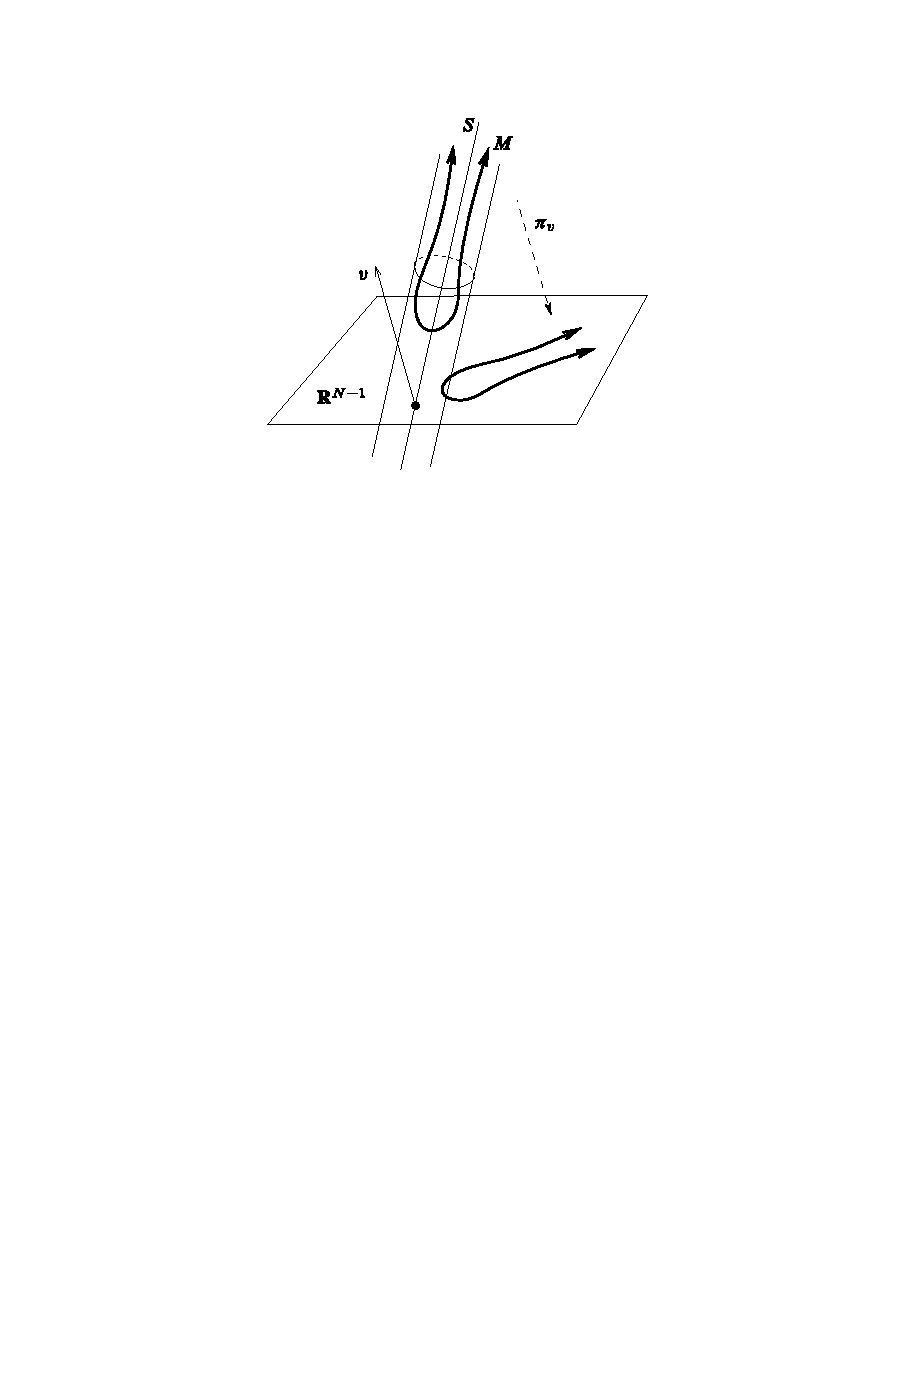
\includegraphics{pictures/Whitney}
\caption{Reducing the codimension of a proper embedding.}
\end{figure}
\begin{proof}
For this proof, given a one-dimensional linear subspace $S\sub\R^N$ and a positive number $R$, let us define the tube with axis $S$ and radius $R$ to be the open subset $T_R(S)\sub\R^N$ consisting of points whose distance from $S$ is less than $R$:
\[T_R(S)=\{x\in\R^N:|x-y|<R\text{ for some $y\in S$}\}\]
Suppose $F:M\to\R^N$ is an arbitrary smooth embedding. Let $G:\R^N\to\B^N$ be a diffeomorphism, and let $f:M\to\R$ be a smooth exhaustion function. Define $\varPsi:M\to\R^N\times\R$ by $\varPsi(p)=(G\circ F(p),f(p))$. Because $G\circ F$ is an embedding, it follows that $\varPsi$ is injective and $d\varPsi_p$ is injective for each $p$, so $\varPsi$ is an injective immersion. It is proper because the preimage of any compact set is a closed subset of the compact set $f^{-1}((-\infty,c])$ for some $c$, so $\varPsi$ is a smooth embedding by Proposition~\ref{smooth embedd if}(b). By construction, the image of $\varPsi$ is contained in
the tube $\B^N\times\R$.\par
Henceforth (after replacing $N+1$ by $N$), we assume that $M$ admits a proper smooth embedding into $\R^N$ for some $N$ that takes its values in some tube $T_R(S)$. Identifying $M$ with its image, we may consider $M$ as a properly embedded submanifold of $\R^N$ contained in the tube.\par
If $N>2n+1$, Lemma~\ref{reduce codim lem} shows that there exists $v\in\R^N-\R^{N-1}$ so that $\pi_v|_M$ is an injective immersion of $M$ into $\R^{N-1}$. Moreover, we may choose $v$ so that it does not lie in the subspace $S$, it follows that $\pi_v(S)$ is a one-dimensional subspace of $\R^{N-1}$, and $\pi_v(M)$ lies in a tube around $\pi_v(S)$ because $\pi_v$ is a bounded linear map. We will show that $\pi_v|_M$ is proper, so it is an embedding by Proposition~\ref{smooth embedd if}(b).\par
Suppose $K\sub\R^{N-1}$ is a compact set. Then $K$ is contained in the open ball around $0$ of some radius $R_1$. For any $x\in\pi_v^{-1}(K)$, there is some $c\in\R$ such that $\pi_v(x)=x-cv$; since $|\pi_v(x)|<R_1$, this means that $x$ is in the tube of radius $R_1$ around the line $\R v$ spanned by $v$. It follows that $M\cap\pi^{-1}_v(K)$ is contained in two tubes, one around $S$ and the other around $\R v$. A simple geometric argument shows that the intersection of two tubes is bounded when their axes are not parallel, so $M\cap\pi^{-1}_v(K)$ is compact. Thus $\pi_v|_M$ is proper, which implies that $\pi_v|_M$ is a properly embedded submanifold of $\R^{N-1}$ contained in a tube. We can now iterate this argument until we achieve a proper smooth embedding of $M$ into $\R^{2n+1}$.
\end{proof}
\begin{theorem}[\textbf{Whitney Embedding Theorem}]
Every smooth $n$-manifold with or without boundary admits a proper smooth embedding into $\R^{2n+1}$.
\end{theorem}
\begin{proof}
Let $M$ be a smooth $n$-manifold with or without boundary. By Lemma~\ref{reduce codim embedd}, it suffices to show that $M$ admits a smooth embedding into some Euclidean space.\par
First suppose $M$ is compact. In this case $M$ admits a finite cover $\{B_1,\dots,B_m\}$ in which each $B_i$ is a regular coordinate ball or half-ball. This means that for each $i$ there exist a coordinate domain $B'_i\sups B_i$ and a smooth coordinate map $\varphi_i:B'_i\to\R^n$ that restricts to a diffeomorphism from $\widebar{B}_i$ to a compact subset of $\R^n$. For each $i$, let $\rho_i:M\to\R$ be a smooth bump function that is equal to $1$ on $\widebar{B}_i$ and supported in $B'_i$. Define a smooth map $F:M\to\R^{nm+m}$ by
\[F(p)=(\rho_1(p)\varphi_1(p),\dots,\rho_m(p)\varphi_m(p),\rho_1(p),\dots,\rho_m(p))\]
where, as usual, $\rho_i$ is extended to be zero away from the support of $\rho_i$. We will show that $F$ is an injective smooth immersion; because $M$ is compact, this implies that $F$ is a smooth embedding.\par
To see that $F$ is injective, suppose $F(p)=F(q)$. Because the sets $B_i$ cover $M$, there is some $i$ such that $p\in B_i$. Then $\rho_i(p)=1$, and the fact that $\rho_i(q)=\rho_i(p)=1$ implies that $q\in\supp(\rho_i)\sub B'_i$, and
\[\varphi_i(q)=\rho_i(q)\varphi_i(q)=\rho_i(p)\varphi_i(p)=\varphi_i(p)\]
Since $\varphi_i$ is injective on $B'_i$, it follows that $p=q$.\par
Next, to see that $F$ is a smooth immersion, let $p\in M$ be arbitrary and choose $i$ such that $p\in B_i$. Because $\rho_i\equiv 1$ on a neighborhood of $p$, we have $d(\rho_i\varphi_i)_p=d(\varphi_i)_p$, which is injective. It follows easily that $dF_p$ is injective. Thus, $F$ is an injective smooth immersion and hence an embedding.\par
The argument above still works when $M$ is an arbitrary compact subset of a larger manifold $\widetilde{M}$ with or without boundary, by covering $M$ with finitely many coordinate balls or half-balls for $\widetilde{M}$. The result is a smooth injective map $F:M\to\R^{nm+m}$ whose differential is injective at each point. Since $M$ is compact, it is therefore a smooth embedding.\par
Now suppose $M$ is noncompact. Let $f:M\to\R$ be a smooth exhaustion function. Sard's theorem shows that for each nonnegative integer $i$, there are regular values $a_i,b_i$ of $f$ such that $i<a_i<b_i<i+1$. Define subsets $D_i,E_i\sub M$ by
\[\begin{array}{ll}
D_0=f^{-1}((-\infty,1]),& E_0=f^{-1}((-\infty,a_1])\\
D_i=f^{-1}([i,i+1]),&E_i=f^{-1}([b_{i-1},a_{i+1}])
\end{array}\]
We have 
\[D_i\sub\Int E_i,\quad M=\bigcup D_i,\quad E_i\cap E_j=\emp\text{ unless $j=i-1,i,i+1$}.\] 
The first part of the proof shows that for each $i$ there is a smooth embedding of $E_i$ into some Euclidean space, and therefore by Lemma~\ref{reduce codim embedd} there is an embedding $\varphi_i:E_i\to\R^{2n+1}$. For each $i$, let $\rho_i:M\to\R$ be a smooth bump function that is equal to $1$ on a neighborhood of $D_i$ and supported in $\Int E_i$, and define $F:\R^{2n+1}\times\R^{2n+1}\times\R$ by
\[F(p)=\Big(\sum_{\text{$i$ is even}}\rho_i(p)\varphi_i(p),\sum_{\text{$i$ is odd}}\rho_i(p)\varphi_i(p),f(p)\Big)\]
Then $F$ is smooth because only one term in each sum is nonzero in a neighborhood of each point, and $F$ is proper because $f$ is. We will show that $F$ is also an injective smooth immersion, hence a smooth embedding.\par
Suppose $F(p)=F(q)$. Then $p\in D_j$ for some $j$, and $f(p)=f(q)$ implies that $q\in D_j$ as well. Arguing just as in the compact case above, we conclude that $p=q$.\par 
Now let $p\in M$ be arbitrary, and choose $j$ such that $p\in D_j$. Then $\rho_j\equiv 1$ on a neighborhood of $p$. Assuming $j$ is odd, for all $q$ in that neighborhood we have
\[F(q)=(\varphi_j(q),\dots,\cdots)\]
which implies that $dF_p$ is injective. A similar argument applies when $j$ is even.
\end{proof}
\begin{corollary}
Every smooth $n$-dimensional manifold with or without boundary is diffeomorphic to a properly embedded submanifold $($with or without boundary$)$ of $\R^{2n+1}$.
\end{corollary}
\begin{corollary}
Suppose $M$ is a compact smooth $n$-manifold with or without boundary. If $N\geq2n+1$, then every smooth map from $M$ to $\R^N$ can be uniformly approximated by embeddings.
\end{corollary}
\begin{proof}
Assume $N\geq2n+1$, and let $f:M\to\R^N$ be a smooth map. By the Whitney embedding theorem, there is a smooth embedding $F:M\to\R^{2n+1}$. The map $G=f\times F:M\to\R^N\times\R^{2n+1}$ is also a smooth embedding, and $f$ is equal to the composition $\pi\circ G$, where $\pi:\R^{N}\times\R^{2n+1}\to\R^N$ is the projection. Let $\widetilde{M}=G(M)\sub\R^N\times\R^{2n+1}$. Lemma~\ref{reduce codim lem} shows that there is a vector $v_{N+2n+1}$ arbitrarily close to $e_{N+2n+1}=(0,\dots,0,1)$ such that $\pi_{v_{N+2n+1}}|_{\widetilde{M}}$ is an embedding. This implies that $\pi_{v_{N+2n+1}}$ is arbitrarily close to $\pi_{e_{N+2n+1}}$. Iterating this, we obtain vectors $v_{N+2n+1},v_{N+2n},\dots,v_{N+1}$ such that $\pi_{v_{N+1}}\circ\cdots\circ\pi_{v_{N+2n+1}}$ restricts to an embedding of $\widetilde{M}$ that is arbitrarily close to $\pi_{e_{N+1}}\circ\cdots\circ\pi_{e_{N+2n+1}}=\pi$, and therefore $\pi_{v_{N+1}}\circ\cdots\circ\pi_{v_{N+2n+1}}\circ G$ is an embedding of $M$ into $\R^N$ that is arbitrarily close to $f$.
\end{proof}
\section{The Whitney approximation theorems}
We would like to find a way to apply the Whitney approximation theorem to produce smooth approximations to continuous maps between smooth manifolds. If $F:N\to M$ is such a map, then by the Whitney embedding theorem we can consider $M$ as an embedded submanifold of some Euclidean space $\R^n$, and approximate $F$ by a smooth map into $\R^n$. However, in general, the image of this smooth map will not lie in $M$. To correct for this, we need to know that there is a smooth retraction from some neighborhood of $M$ onto $M$. For this purpose, we introduce tubular neighborhoods.\par
We begin with a theorem about smoothly approximating functions into Euclidean spaces. Our first theorem shows, in particular, that any continuous function from a
smooth manifold $M$ into $\R^k$ can be uniformly approximated by a smooth function. In fact, we will prove something stronger. If $\delta:M\to\R$ is a positive continuous function, we say that two functions $F,\widetilde{F}:M\to\R^k$ are \textbf{$\bm{\delta}$-close} if $|F(x)-\widetilde{F}(x)|<\delta(x)$ for all $x\in M$.
\begin{theorem}[\textbf{Whitney Approximation Theorem for Functions}]\label{Whitney appox function}
Suppose $M$ is a smooth manifold with or without boundary, and $F:M\to\R^k$ is a continuous function. Given any positive continuous function $\delta:M\to\R$, there exists a smooth function $\widetilde{F}:M\to\R^k$ that is $\delta$-close to $F$. If $F$ is smooth on a closed subset $A\sub M$, then $\widetilde{F}$ can be chosen to be equal to $F$ on $A$.
\end{theorem}
\begin{proof}
If $F$ is smooth on the closed subset $A$, then by the extension lemma for smooth functions (Lemma~\ref{ext lem smooth func}), there is a smooth function $F_0:M\to\R^k$ that agrees with $F$ on $A$. Let 
\[U_0=\{y\in M:|F_0(y)-F(y)|<\delta(y)\}\]
Then $U_0$ is an open subset containing $A$. (If there is no such set $A$, we just take $U_0=A=\emp$ and $F_0\equiv0$.)\par
We will show that there are countably many points $\{x_i\}_{i=1}^{\infty}$ in $M-A$ and neighborhoods $U_i$ of $x_i$ in $M-A$ such that $\{U_i\}_{i=1}^{\infty}$ is an open cover of $M-A$ and
\begin{align}\label{Whitney appox-1}
|F(y)-F(x_i)|<\delta(y)\quad\text{for all }y\in U_i
\end{align}
To see this, for any $x\in M-A$, let $U_x$ be a neighborhood of $x$ contained in $M-A$ and small enough that
\[\delta(y)>\frac{1}{2}\delta(x)\And |F(y)-F(x)|<\frac{1}{2}\delta(x)\]
for all $y\in U_x$. Then if $y\in U_x$, we have \[|F(y)-F(x)|<\frac{1}{2}\delta(x)<\frac{1}{2}\delta(y)\]
The collection $\{U_x:x\in M-A\}$ is an open cover of $M-A$. Choosing a countable subcover $\{U_{x_i}\}_{i=1}^{\infty}$ and setting $U_i=U_{x_i}$, we have $(\ref{Whitney appox-1})$.\par
Let $\{\varphi_0,\varphi_i\}$ be a smooth partition of unity subordinate to the cover $\{U_0,U_i\}$ of $M$, and define $\widetilde{F}:M\to\R^k$ by
\[\widetilde{F}(y)=\varphi_0(y)F_0(y)+\sum_{i\geq 1}\varphi_i(y)F(x_i)\]
Then clearly $\widetilde{F}$ is smooth, and is equal to $F$ on $A$. For any $y\in M$, the fact that $\sum_{i\geq 0}\varphi_i\equiv 1$ implies that
\begin{align*}
|\widetilde{F}(y)-F(y)|&=\Big|\varphi_0(y)F_0(y)+\sum_{i\geq 1}\varphi_i(y)F(x_i)-\Big(\varphi_0+\sum_{i\geq 1}\varphi_i(y)\Big)F(y)\Big|\\
&\leq\varphi_0(y)|F_0(y)-F(y)|+\sum_{i\geq 1}\varphi_i(y)|F(y)-F(x_i)|\\
&<\varphi_0(y)\delta(y)+\sum_{i\geq 1}\varphi_i(y)\delta(y)=\delta(y)
\end{align*}
\end{proof}
\begin{corollary}\label{appox positive function}
If $M$ is a smooth manifold with or without boundary and $\delta:M\to\R$ is a positive continuous function, there is a smooth function $e:M\to\R$ such that $0<e(x)<\delta(x)$ for all $x\in M$.
\end{corollary}
\begin{proof}
Use the Whitney approximation theorem to construct a smooth function $e:M\to\R$ that satisfies
\[|e(x)-\frac{1}{2}\delta(x)|<\frac{1}{2}\delta(x)\]
for all $x\in M$.
\end{proof}
\section{Tubular neighborhoods}
For each $x\in\R^n$, the tangent space $T_x\R^n$ is canonically identified with $\R^n$ itself, and the tangent bundle $T\R^n$ is canonically diffeomorphic to $\R^n\times\R^n$. By virtue of this identification, each tangent space $T_x\R^n$ inherits a Euclidean dot product. Suppose $M\sub\R^n$ is an embedded $m$-dimensional submanifold. For each $x\in M$, we define the normal space to $M$ at $x$ to be the $(n-m)$-dimensional subspace $N_xM\sub T_x\R^n$ consisting of all vectors that are orthogonal to $T_xM$ with respect to the Euclidean dot product. The normal bundle of $M$, denoted by $NM$, is the subset of $T\R^n\approx\R^n\times\R^n$ consisting of vectors that are normal to $M$:
\[NM=\{(x,v):x\in M,v\in N_xM\}\]
There is a natural projection $\pi:NM\to M$ defined as the restriction to $NM$ of $\pi:T\R^n\to\R^n$.
\begin{theorem}
If $M\sub\R^n$ is an embedded $m$-dimensional submanifold, then $NM$ is an embedded $n$-dimensional submanifold of $T\R^n\approx\R^n\times\R^n$.
\end{theorem}
\begin{proof}
Let $x_0$ be any point of $M$, and let $(U,\varphi)$ be a slice chart for $M$ in $\R^n$ centered at $x_0$. Write $\widehat{U}=\varphi(U)\sub\R^n$, and write the coordinate functions of $\varphi$ as $(u^1,\dots,u^n)$, so that $M\cap U$ is the set where $\{u^{m+1}=\cdots=u^n=0\}$. At each point $x\in U$, the vectors $E_j|_x:=(d\varphi_x)^{-1}(\partial/\partial u^j|_{\varphi(x)})$ form a basis for $T_x\R^n$. We can expand each $E_j|_x$ in terms of the standard coordinate frame as
\[E_j|_x=E^i_j(x)\frac{\partial}{\partial x^i}\Big|_x\]
where each $E^i_j(x)$ is a partial derivative of $\varphi^{-1}$ evaluated at $\varphi(x)$, and thus is a smooth function of $x$.\par
Define a smooth function $\varPhi:U\times\R^n\to\widehat{U}\times\R^n$ by
\[\varPhi(u,v)=\big(u^1(x),\dots,u^n(x),(v,E_1|_x),\dots,(v,E_n|_x)\big)\]
The total derivative of $\varPhi$ at a point $(x,v)$ is
\[\partial\varPhi(x,v)=\begin{pmatrix}
\frac{\partial u^i}{\partial x^j}(x)&0\\
*&E^i_j(x)
\end{pmatrix}\]
which is invertible, so $\varPhi$ is a local diffeomorphism. If $\varPhi(x,v)=\varPhi(y,w)$, then $x=y$ because $\varphi$ is injective, and then the fact that $(v,E_i|_x)=(w,E_i|_x)$ for each $i$ implies that $v=w$. Thus $\varPhi$ is injective, so it defines a smooth coordinate chart on $U\times\R^n$. The definitions imply that $(x,v)\in NM$ if and only if $\varPhi(x,v)$ is in the slice
\[\{(y,z)\in\R^n\times\R^n:y^{m+1}=\cdots=y^n=0,z^1=\cdots=z^m=0\}\]
Thus $\varPhi$ is a slice chart for $NM$ in $\R^n\times\R^n$.
\end{proof}
Thinking of $NM$ as a submanifold of $\R^n\times\R^n$, we define $E:NM\to\R^n$ by
\[E(x,v)=(x+v)\]
This maps each normal space $N_xM$ affinely onto the affine subspace through $x$ and orthogonal to $T_xM$. Clearly, $E$ is smooth, because it is the restriction to $NM$ of the addition map $\R^n\times\R^n\to\R^n$. A \textbf{tubular neighborhood of $\bm{M}$} is a neighborhood $U$ of $M$ in $\R^n$ that is the diffeomorphic image under $E$ of an open subset $V\sub NM$ of the form
\begin{align}\label{tubular}
V=\{(x,v)\in NM:|v|<\delta(x)\}
\end{align}
for some positive continuous function $\delta:M\to\R$.
\begin{theorem}[\textbf{Tubular Neighborhood Theorem}]\label{Euclidean tubular neighborhood}
Every embedded submanifold of $\R^n$ has a tubular neighborhood.
\end{theorem}
\begin{proof}
Let $M_0\sub NM$ be the subset $\{(x,0):x\in M\}$. We begin by showing that $E$ is a local diffeomorphism on a neighborhood of $M_0$. By the inverse function theorem, it suffices to show that the differential $dE_{(x,0)}$ is bijective at each point $(x,0)\in M_0$. This follows easily from the following two facts: 
\begin{itemize}
\item The restriction of $E$ to $M_0$ is the obvious diffeomorphism $M_0\to M$, so $dE_{(x,0)}$ maps the subspace $T_{(x,0)}M_0\sub T_{(x,0)}NM$ isomorphically onto $T_xM$.
\item The restriction of $E$ to the fiber $N_xM$ is the affine map $w\mapsto x+w$, so $dE_{(x,0)}$ maps $T_{(x,0)}(N_xM)$ isomorphically onto $N_xM$.
\end{itemize}  
Since $T_x\R^n=T_xM\oplus N_xM$, these together show that $dE_{(x,0)}$ is surjective, and hence is bijective for dimensional reasons. Thus, $E$ is a diffeomorphism on a neighborhood of $(x,0)$ in $NM$, which we can take to be of the form $V_\delta(x)=\{(y,w)\in NM:|x-y|<\delta,|w|<\delta\}$ for some $\delta>0$.\par
To complete the proof, we need to show that there is an open subset $V$ of the form $(\ref{tubular})$ on which $E$ is a global diffeomorphism. For each point $x\in M$, let 
\[\rho(x)=\sup\{\delta<1:E\text{ is a diffeomorphism from $V_\delta(x)$ to its image}\}\]
The argument in the preceding paragraph implies that $\rho:M\to\R$ is positive.
\begin{figure}[htbp]
\centering
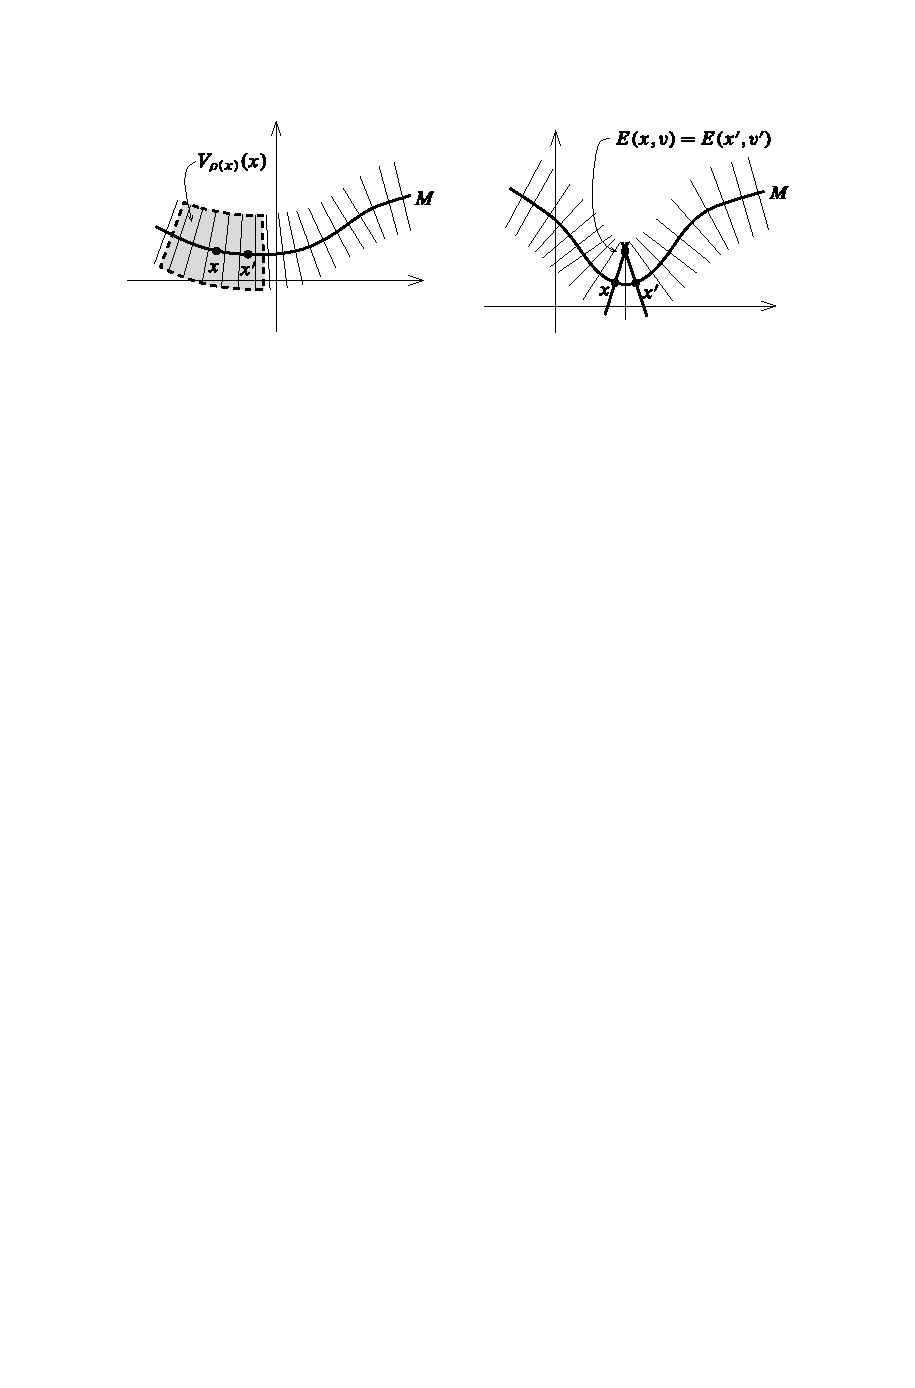
\includegraphics{pictures/tubular}
\caption{Continuity of $\rho$ and Injectivity of $E$.}
\end{figure}\par
To show it is continuous, let $x,y\in M$ be arbitrary, and suppose first that $|x-y|<\rho(x)$. Then by the triangle inequality, $V_\delta(y)$ is 
contained in $V_{\rho(x)}(x)$ for $\delta=\rho(x)-|x-y|$, which implies that $\rho(y)\geq\rho(x)-|x-y|$, or
\[\rho(x)-\rho(y)\leq|x-y|.\]

On the other hand, if $|x-y|\geq\rho(x)$, then the inequality above holds for trivial reasons. Reversing the roles of $x$ and $y$ yields an analogous inequality, which shows that $|\rho(x)-\rho(y)|\leq|x-y|$, so $\rho$ is continuous.\par
Now let $V=\{(x,v)\in NM:|v|<1/2\rho(x)\}$. We will show that $E$ is injective on $V$. Suppose that $(x,v)$ and $(y,w)$ are points in $V$ such that $E(x,v)=E(y,w)$. Assume without loss of generality that $\rho(x)\leq\rho(y)$. It follows from $x+v=y+w$ that
\[|x-y|=|v-w|\leq|v|+|w|\leq\frac{1}{2}\rho(x)+\frac{1}{2}\rho(y)\leq\rho(x)\]
Therefore, both $(x,v)$ and $(y,w)$ are in $V_{\rho(x)}(x)$. Since $(x,v)$ and $(y,w)$ are then in $V_\delta(x)$ for some $\delta<\rho(x)$ and $E$ is injective on $V_\delta(x)$, this implies $(x,v)=(y,w)$.\par
The set $U=E(V)$ is open in $\R^n$ because $E|_V$ is a local diffeomorphism and thus an open map. It follows that $E:V\to U$ is a smooth bijection and a local diffeomorphism, hence a diffeomorphism by Proposition~\ref{local diff prop}. Therefore, $U$ is a tubular neighborhood of $M$.
\end{proof}
One of the most useful features of tubular neighborhoods is expressed in the next proposition. A \textbf{retraction} of a topological space $X$ onto a subspace $M\sub X$ is a continuous map $r:X\to M$ such that $r|_M$ is the identity map of $M$.
\begin{proposition}\label{tubular retraction}
Let $M\sub\R^n$ be an embedded submanifold. If $U$ is any tubular neighborhood of $M$, there exists a smooth map $r:U\to M$ that is both a retraction and a smooth submersion.
\end{proposition}
\begin{proof}
Let $NM\sub T\R^n$ be the normal bundle of $M$, and let $M_0\sub NM$ be the set $M_0=\{(x,0):x\in M\}$. By the definition of a tubular neighborhood, there is an open 
subset $V\sub NM$ containing $M_0$ such that $E:V\to U$ is a diffeomorphism. Define $r:U\to M$ by $r=\pi_{NM}\circ E^{-1}$, where $\pi_{NM}:NM\to M$ is the natural
projection. Then $r$ is smooth by composition. For $x\in M$, note that $E(x,0)=x$, so $r(x)=\pi\circ E(x)=\pi(x,0)=x$, which shows that $r$ is a retraction. Since 
$\pi$ is a smooth submersion and $E^{-1}$ is a diffeomorphism, it follows that $r$ is a smooth submersion.
\end{proof}
\section{Smooth approximation of maps between manifolds}
Now we can extend the Whitney approximation theorem to maps between manifolds.
\begin{theorem}[\textbf{Whitney Approximation Theorem}]\label{Whitney approximation}
Suppose $N$ is a smooth manifold with or without boundary, $M$ is a smooth manifold $($without boundary$)$, and $F:N\to M$ is a continuous map. Then $F$ is homotopic to a smooth map. If $F$ is already smooth on a closed subset $A\sub N$, then the homotopy can be taken to be relative to $A$.
\end{theorem}
\begin{proof}
By the Whitney embedding theorem, we may as well assume that $M$ is a properly embedded submanifold of $\R^n$. Let $U$ be a tubular neighborhood of $M$ in $\R^n$, and let $r:U\to M$ be the smooth retraction given by Proposition~\ref{tubular retraction}. For any $x\in M$, let
\begin{align*}
\delta(x)=\sup\{\eps\leq 1:\B(x,\eps)\sub U\}
\end{align*}
By a triangle-inequality argument just like the one in the proof of the tubular neighborhood theorem, $\delta:M\to\R^+$ is continuous. Let $\tilde{\delta}=\delta\circ F:N\to\R^+$. By Theorem~\ref{Whitney appox function}, there exists a smooth function $\widetilde{F}:N\to\R^n$ that is $\tilde{\delta}$-close to $F$, and is equal to $F$ on $A$ (which might be the empty set). Let $H:N\times I\to M$ be the composition of $r$ with the straight-line homotopy between $F$ and $\widetilde{F}$:
\[H(p,t)=r\big((1-t)F(p)+t\widetilde{F}(p)\big)\]
This is well defined, because our condition on $\widetilde{F}$ guarantees that for each $p\in N$, $|\widetilde{F}(p)-F(p)|<\tilde{\delta}(p)=\delta(F(p))$, which means that $\widetilde{F}(p)$ is contained in the ball of radius $\delta(F(p))$ around $F(p)$; since this ball is contained in $U$, so is the entire line segment from $F(p)$ to $\widetilde{F}(p)$.\par
Thus $H$ is a homotopy between $H(p,0)=F(p)$ and $H(p,1)=r\circ\widetilde{F}(p)$ which is a smooth map by composition. It satisfies $H(p,t)=F(p)$ for all $p\in A$, since $F=\widetilde{F}$ there.
\end{proof}
\begin{corollary}[\textbf{Extension Lemma for Smooth Maps}]
Suppose $N$ is a smooth manifold with or without boundary, $M$ is a smooth manifold, $A\sub N$ is a closed subset, and $f:A\to M$ is a smooth map. Then $f$ has a smooth extension to $N$ if and only if it has a continuous extension to $N$.
\end{corollary}
\begin{proof}
If $F:N\to M$ is a continuous extension of $f$ to all of $N$, the Whitney approximation theorem guarantees the existence of a smooth map $\widetilde{F}$ (homotopic to $F$, in fact, though we do not need that here) that agrees with $f$ on $A$, in other words, $\widetilde{F}$ is a smooth extension of $f$. The converse is obvious.
\end{proof}
If $N$ and $M$ are two smooth manifolds with or without boundary, a homotopy $H:N\times I\to M$ is called a \textbf{smooth homotopy} if it is also a smooth map, in the sense that it extends to a smooth map on some neighborhood of $N\times I$ in $N\times\R$. Two maps are said to be \textbf{smoothly homotopic} if there is a smooth homotopy between them.
\begin{lemma}\label{smooth homotopy trans}
If $N$ and $M$ are smooth manifolds with or without boundary, smooth homotopy is an equivalence relation on the set of all smooth maps from $N$ to $M$.
\end{lemma}
\begin{proof}
Reflexivity and symmetry are proved just as for ordinary homotopy. To prove transitivity, suppose $F,G,K:N\to M$ are smooth maps, and $H_1,H_2:N\times I\to M$ are smooth homotopies from $F$ to $G$ and from $G$ to $K$, respectively. Let $\varphi:[0,1]\to[0,2]$ be a smooth map such that 
\[\left\{\begin{array}{l}
\varphi(0)=0,\varphi(1)=2,\\
0\leq\varphi(t)\leq 1,\ t\in[0,1/2]\\
1\leq\varphi(t)\leq 2,\ t\in[1/2,1]\\
\varphi(t)\equiv 1\text{ in a neighborhood of }1/2.
\end{array}\right. \]
Define $H:N\times I\to M$ by
\[H(x,t)=\begin{cases}
H_1(x,\varphi(t)),&t\in[0,1/2]\\
H_2(x,\varphi(t)-1),&t\in[1/2,1]
\end{cases}\]
Then it is easy to check that $H$ is a smooth homotopy from $F$ to $K$.
\end{proof}
\begin{theorem}\label{homotopy to smooth}
Suppose $N$ is a smooth manifold with or without boundary, $M$ is a smooth manifold, and $F,G:N\to M$ are smooth maps. If $F$ and $G$ are homotopic, then they are smoothly homotopic. If $F$ and $G$ are homotopic relative to some closed subset $A\sub N$, then they are smoothly homotopic relative to $A$.
\end{theorem}
\begin{proof}
Suppose $F,G:N\to M$ are smooth, and let $H:N\times I\to M$ be a homotopy from $F$ to $G$ (relative to $A$, which may be empty). We wish to show that $H$ can be replaced by a smooth homotopy.\par
Define $\widebar{H}:N\times I\to M$ by
\[\widebar{H}(x,t)=\begin{cases}
H(x,0),&t\leq 0\\
H(x,t),&t\in[0,1]\\
H(x,1),&t\geq 1
\end{cases}\]
This is continuous by the gluing lemma. The restriction of $\widebar{H}$ to $(N\times\{0\})\cup(N\times\{1\})$ is smooth, because it is equal to $F\circ\pi_1$ on $N\times\{0\}$ and $G\circ\pi_1$ on $N\times\{1\}$ (where $\pi_1:N\times I\to N$ is the projection). If $H$ is a homotopy relative to $A$, then $\widebar{H}$ is also smooth on $A\times I$. Because $N\times\R$ is a smooth manifold with (possibly empty) boundary, the Whitney approximation theorem guarantees that there is a smooth
map $\widetilde{H}:N\times\R\to M$ (homotopic to $\widetilde{H}$, but we do not need that here) whose restriction to $(N\times\{0\})\cup(N\times\{1\})\cup(A\times I)$ agrees with $\widebar{H}$ (and therefore $H$). Restricting back to $N\times I$ again, we see that $\widetilde{H}|_{N\times I}$ is a smooth homotopy (relative to $A$) between $F$ and $G$.
\end{proof}
\section{Transversality}
As our final application of Sard‘s theorem, we show how submanifolds can be perturbed so that they intersect nicely. To explain what this means, we introduce the
concept of \textit{transversality}.\par
The intersection of two linear subspaces of a vector space is always another linear subspace. The analogous statement for submanifolds is certainly not true: it is easy to come up with examples of smooth submanifolds whose intersection is not a submanifold. But with an additional assumption about the submanifolds, it is possible to show that their intersection is again a submanifold.\par
Suppose $M$ is a smooth manifold. Two embedded submanifolds $S,S'\sub M$ are said to \textbf{intersect transversely} if for each $p\in S\cap S'$, the tangent spaces $T_pS$ and $T_pS'$ together span $T_pM$ (where we consider $T_pS$ and $T_pS'$ as subspaces of $T_pM$).\par
For many purposes, it is more convenient to work with the following more general definition. If $F:N\to M$ is a smooth map and $S\sub M$ is an embedded submanifold,
we say that $F$ is \textbf{transverse to $\bm{S}$} if for every $x\in F^{-1}(S)$, the spaces $T_{F(x)}S$ and $dF_x(T_xN)$ together span $T_{F(x)}M$. One special case is worth noting: if $F$ is a smooth submersion, then it is automatically transverse to every embedded submanifold of $M$. Two embedded submanifolds intersect transversely if and only if the inclusion of either one is transverse to the other.\par
The next result, a generalization of the regular level set theorem, shows why transversality is desirable.
\begin{theorem}\label{transverse intersection preimage subm}
Suppose $N$ and $M$ are smooth manifolds and $S\sub M$ is an embedded submanifold.
\begin{itemize}
\item[(a)]If $F:N\to M$ is a smooth map that is transverse to $S$, then $F^{-1}(S)$ is an embedded submanifold of $N$ whose codimension is equal to the codimension of $S$ in $M$. Moreover, for each $p\in F^{-1}(S)$, we have $T_p(F^{-1}(S))=(dF_p)^{-1}(T_{F(p)}S)$.
\item[(b)]If $S'\sub M$ is an embedded submanifold that intersects $S$ transversely, then $S\cap S'$ is an embedded submanifold of $M$ whose codimension is equal to the sum of the codimensions of $S$ and $S'$. Moreover, for each $p\in S\cap S'$ we have $T_{p}(S\cap S')=T_pS\cap T_{p}S'$.
\end{itemize}
\end{theorem}
\begin{proof}
The second statement follows easily from the first, simply by taking $F$ to be the inclusion map $S'\hookrightarrow M$, and noting that a composition of smooth embeddings $S\cap S'\hookrightarrow S'\hookrightarrow M$ is again a smooth embedding.\par
To prove (a), let $m$ denote the dimension of $M$ and $k$ the codimension of $S$ in $M$. Given $x\in F^{-1}(S)$, we can find a neighborhood $U$ of $F(x)$ in $M$ and a local defining function $\varphi:U\to\R^k$ for $S$, with $S\cap U=\varphi^{-1}(0)$. The theorem will be proved if we can show that $0$ is a regular value of $\varphi\circ F$, because $F^{-1}(S)\cap F^{-1}(U)$ is the zero set of $\varphi\circ F|_{F^{-1}(U)}$.\par
Given $z\in T_0\R^k$ and $p\in(\varphi\circ F)^{-1}(0)$, the fact that $0$ is a regular value of $\varphi$ means there is a vector $y\in T_{F(p)}M$ such that $d\varphi_{F(p)}(y)=z$. The fact that $F$ is transverse to $S$ means we can write $y=y_0+dF_p(v)$ for some $y_0\in T_{F(p)}S$ and some $v\in T_pN$. Because $\varphi$ is constant on $S\cap U$, it follows that $d\varphi_{F(p)}(y_0)=0$, so
\[d(\varphi\circ F)_p(v)=d\varphi_{F(p)}(dF_p(v))=d\varphi_{F(p)}(y_0+dF_p(v))=d\varphi_{F(p)}(y)=z.\]
Thus $F^{-1}(S)$ is an embedded submanifold of codimension $k$.\par
Finally, let $p\in F^{-1}(S)$. Choose a neighborhood $U$ of $F(p)$ and a local defining function $\varPhi:U\to N$ for $S$. Then we have $T_{F(p)}S=\ker d\varPhi_{F(p)}$. By the definition of a local defining function, $\varPhi\circ F$ is constant on $F^{-1}(S)\cap F^{-1}(U)$, and therefore $d\varPhi_{F(p)}\circ dF_p$ is zero on $T_p(F^{-1}(S))$. This then means $ dF_p(T_p(F^{-1}(S)))\sub\ker d\varPhi_{F(p)}S$, and by dimension consideration they are equal. Combining the previous observation, we obtain $\im dF_p=T_{F(p)}S$, and so $T_p(F^{-1}(S))=(dF_p)^{-1}(T_{F(p)}S)$.
\end{proof}
For example, in $\R^3$, this theorem shows that a smooth curve and a smooth surface intersecting transversely have only isolated points in their intersection, while two smooth surfaces intersect transversely in a smooth curve. Two smooth curves in $\R^3$ intersect transversely if and only if their intersection is empty, because at any intersection point, the two one-dimensional tangent spaces to the curves would have to span the tangent space to $\R^3$.\par 
Because a submersion is transverse to every embedded submanifold, the next corollary is immediate.
\begin{corollary}
Suppose $N$ and $M$ are smooth manifolds, $S\sub M$ is an embedded submanifold of codimension $k$, and $F:N\to M$ is a submersion. Then $F^{-1}(S)$ is an embedded codimension-$k$ submanifold of $N$.
\end{corollary}
Transversality also provides a convenient criterion for recognizing a submanifold as a graph. The next theorem is a global version of the implicit function theorem.
\begin{theorem}[\textbf{Global Characterization of Graphs}]\label{char graph}
Suppose $M$ and $N$ are smooth manifolds and $S\sub M\times N$ is an immersed submanifold. Let $\pi_M$ and $\pi_N$ denote the projections from $M\times N$ onto $M$ and $N$, respectively. The following are equivalent.
\begin{itemize}
\item[(\rmnum{1})]$S$ is the graph of a smooth map $f:M\to N$.
\item[(\rmnum{2})]$\pi_M|_S$ is a diffeomorphism from $S$ onto $M$.
\item[(\rmnum{3})]For each $p\in M$, the submanifolds $S$ and $\{p\}\times N$ intersect transversely in exactly one point.
\end{itemize}
If these conditions hold, then $S$ is the graph of the map $f:M\to N$ defined by $f=\pi_N\circ(\pi_M|_S)^{-1}$.
\end{theorem}
\begin{proof}
The implication $(\rmnum{1})\Rightarrow(\rmnum{2})$ is clear. For $(\rmnum{2})\Rightarrow(\rmnum{1})$, we can simply define $f=\pi_N\circ(\pi_M|_S)^{-1}$.\par
Now we show $(\rmnum{2})\Rightarrow(\rmnum{3})$. Assume $\pi_M|_S$ has an smooth inverse $(\pi_M|_S)^{-1}$. In this case, each slice $\{p\}\times N$ only intersects $S$ at $(p,(\pi_M|_S)^{-1}(p))$. At each point $(p,q)$ of $M\times N$, the tangent space $T_{(p,q)}(M\times N)=T_pM\oplus T_qN$, with $T_pM=\ker d(\pi_N)_p$ and $T_qN=\ker d(\pi_M)_q$. Now for any point $(p,q)\in S$, the map $\pi_M|_S$ is a diffeomorphism from $S$ onto $M$, therefore we have $T_{(p,q)}(M\times N)=T_pM\oplus\ker d(\pi_M|_S)_p=T_pM\oplus T_qN$. Since $T_qN$ is the tangent space of $\{p\}\times N$ at $(p,q)$, it follows that $S$ intersects transversely with $\{p\}\times N$.\par
For the part $(\rmnum{3})\Rightarrow(\rmnum{2})$. If $S$ intersects $p\times\{N\}$ in exactly one point for each $p\in M$, then the projection $\pi_M|_S$ is bijective. Also, from the transversality we can see it is a submersion, hence is a diffeomorphism.
\end{proof}
\begin{corollary}[\textbf{Local Characterization of Graphs}]\label{char graph local}
Suppose $M$ and $N$ are smooth manifolds, $S\sub M\times N$ is an immersed submanifold, and $(p,q)\in S$. If $S$ intersects the submanifold $\{p\}\times N$ transversely at $(p,q)$, then there exist a neighborhood $U$ of $p$ in $M$ and a neighborhood $V$ of $(p,q)$ in $S$ such that $V$ is the graph of a smooth map $f:U\to N$.
\end{corollary}
\begin{proof}
The hypothesis guarantees that $d(\pi_M)_{(p,q)}:T_{(p,q)}S\to T_pM$ is an isomorphism, so $\pi_M|_S$ restricts to a diffeomorphism from a neighborhood $V$ of $(p,q)$ in $S$ to a neighborhood $U$ of $p$. The result then follows from Theorem~\ref{char graph}(\rmnum{2}).
\end{proof}
Suppose $N,M$ and $S$ are smooth manifolds, and for each $s\in S$ we are given a map $F_s:N\to M$. The collection $\{F_s:s\in S\}$ is called a \textbf{smooth family of maps} if the map $F:N\times S\to M$ defined by $F(x,s)=F_s(x)$ is smooth. You should think of such a family as a higher-dimensional analogue of a homotopy. The next proposition shows how such families are related to ordinary homotopies.
\begin{proposition}\label{smooth family map homotopy}
If $\{F_s:s\in S\}$ is a smooth family of maps from $N$ to $M$ and $S$ is connected, then for any $s_1,s_2\in S$, the maps $F_{s_1},F_{s_2}:N\to M$ are homotopic.
\end{proposition}
\begin{proof}
Because $S$ is connected, it is path-connected. If $\gamma:[0,1]\to S$ is any path from $s_1$ to $s_2$, then $H(x,s)=F(x,\gamma(s))$ is a homotopy from $F_{s_1}$ to $F_{s_2}$.
\end{proof}
The key to finding transversemaps is the following application of Sard's theorem, which gives a simple sufficient condition for a family of smooth maps to contain at least one map that is transverse to a given submanifold. If $S$ is a smooth manifold and $B\sub S$ is a subset whose complement has measure zero in $S$, we say that $B$ contains \textbf{almost every element} of $S$.
\begin{theorem}[\textbf{Parametric Transversality Theorem}]\label{parametric transversality}
Suppose $N$ and $M$ are smooth manifolds, $X\sub M$ is an embedded submanifold, and $\{F_s:s\in S\}$ is a smooth family of maps from $N$ to $M$. If the map $F:N\times S\to M$ is transverse to $X$, then for almost every $s\in S$, the map $F_s:N\to M$ is transverse to X.
\end{theorem}
\begin{proof}
The hypothesis implies that $W=F^{-1}(X)$ is an embedded submanifold of $N\times S$ by Theorem~\ref{transverse intersection preimage subm}. Let $\pi:N\times S\to S$ be the projection onto the second factor. What we will actually show is that if $s\in S$ is a regular value of the restriction $\pi|_W$, then $F_s$ is transverse to $X$. Since almost every $s$ is a regular value by Sard's theorem, this proves the theorem.\par
Suppose $s\in S$ is a regular value of $\pi|_W$. Let $p\in F_s^{-1}(X)$ be arbitrary, and set $q=F_s(p)\in X$. We need to show that $T_qM=T_qX+d(F_s)(T_pN)$. Let $\iota_1:N\to N\times S$ and $\iota_2:S\to N\times S$ be defined by
\[\iota_1(p')=(p',s),\quad \iota_2(s')=(p,s').\]
Then by our hypothesis on $F$, we have
\begin{align*}
T_qM&=T_qX+dF(T_{(p,s)}(N\times S))=T_qX+dF(d\iota_1(T_pN)+d\iota_2(T_sS))\\
&=T_qX+d(F\circ\iota_1)(T_pN)+d(F\circ\iota_2)(T_sS)=T_qX+d(F_s)(T_pN)+d(F\circ\iota_2)(T_sS).
\end{align*}
Since $s$ is a regular value of $\pi|_W$, we have $T_sS=d\pi(T_{(p,s)}W)$. Insert this into the equation above, we obtain
\begin{align}\label{parametric transversality-1}
T_qM=T_qX+d(F_s)(T_pN)+dF\circ d(\iota_2\circ\pi)(T_{(p,s)}W).
\end{align}
Note that the map $\iota_2\circ\pi$ sends a point $(p',s')$ in $N\times S$ to $(p,s')$, so it is the identity on the second factor. We may conclude, from this and the fact $d\pi(T_{(p,s)}W)=T_sS$ that
\begin{align}\label{parametric transversality-2}
d(\iota_p\circ\pi)(T_{(p,s)}W)=V_p+d(\iota_2)(T_sS),
\end{align}
where $V_p\sub d(\iota_1)(T_pN)$. Combining $(\ref{parametric transversality-1})$ and $(\ref{parametric transversality-2})$, we then get
\begin{align*}
T_qM&=T_qX+d(F_s)(T_pN)+dF(V_p+d(\iota_2)(T_sS))\\
&=T_qX+d(F_s)(T_pN)+d(F\circ\iota_2)(T_sS)+dF(V_p)\\
&\sub T_qX+d(F_s)(T_pN)+d(F\circ\iota_2)(T_sS)+d(F\circ\iota_1)(T_pN)\\
&=T_qX+d(F_s)(T_pN)+dF(T_{(p,s)}W)\\
&=T_qX+d(F_s)(T_pN)+T_qX=T_qX+d(F_s)(T_pN).
\end{align*}
This finishes the proof.
\end{proof}
In order to make use of the parametric transversality theorem, we need to construct
a smooth family of maps satisfying the hypothesis. The proof of the next
theorem shows that it is always possible to do so.
\begin{theorem}[\textbf{Transversality Homotopy Theorem}]
Suppose $M$ and $N$ are smooth manifolds and $X\sub M$ is an embedded submanifold. Every smooth map $f:N\to M$ is homotopic to a smooth map $g:N\to M$ that is transverse to $X$.
\end{theorem}
\begin{proof}
We will construct a smooth map $F:N\times S\to M$ that is transverse to $X$, where $S=\B^k$ for some $k$ and $F_0=f$. It then follows from the parametric transversality theorem that there is some $s\in S$ such that $F_s:N\to M$ is transverse to $X$, and from Proposition~\ref{smooth family map homotopy} that $F_s$ is homotopic to $f$.\par
By theWhitney embedding theorem, we can assume thatM is a properly embedded
submanifold of $\R^k$ for some $k$. Let $U$ be a tubular neighborhood of $M$ in $\R^k$, and let $r:U\to M$ be a smooth retraction that is also a smooth submersion. If we define $\delta:U\to\R^+$ by 
\begin{align*}
\delta(x)=\sup\{\eps\leq 1:\B(x,\eps)\sub U\},
\end{align*}
then Corollary~\ref{appox positive function} shows that there exists a smooth function $e:N\to\R^+$ that satisfies $0<e(p)<\delta(f(p))$ everywhere. Let $S$ be the unit ball in $\R^k$, and define $F:N\times S\to M$ by
\[F(p,s)=r(f(p)+e(p)s).\]
Note that $|e(p)s|<e(p)<\delta(f(p))$, which implies that $f(p)+e(p)s\in U$, so $F$ is well defined. Clearly, $F$ is smooth, and $F_0=f$ because $r$ is a retraction.\par
For each $p\in N$, the restriction of $F$ to $\{p\}\times S$ is the composition of the local diffeomorphism $s\mapsto f(p)+e(p)s$ followed by the smooth submersion $r$, so $F$ is a smooth submersion and hence transverse to $X$.
\end{proof}
\section{Exercise}
\begin{exercise}
Let $M$ be a smooth manifold, let $B\sub M$ be a closed subset, and let $\delta:M\to\R$ be a positive continuous function. Show that there is a smooth function $\tilde{\delta}:M\to\R$ that is zero on $B$, positive on $M-B$, and satisfies $\tilde{\delta}<\delta(x)$ everywhere.
\end{exercise}
\begin{proof}
Consider $f/(f+1)$, where $f$ is a smooth nonnegative function that vanishes exactly on $B$. By applying Corollary~\ref{appox positive function} to $f\delta/(f+1)$ we get a smooth function $\tilde{\delta}:M-B\to\R$ such that 
\[\tilde{\delta}<\frac{\delta f}{f+1}<\delta\]
Now $\tilde{\delta}(x)=0$ if $x\in B$.
\end{proof}
\begin{exercise}
Let $M$ be a smooth manifold, let $B$ be a closed subset of $M$, and let $\delta:M\to\R$ be a positive continuous function.
\begin{itemize}
\item[(a)]Given any continuous function $f:M\to\R^k$, show that there is a continuous function $\widetilde{f}:M\to\R^k$ that is smooth on $M-B$, agrees with $f$ on $B$, and is $\delta$-close to $f$.
\item[(b)]Given a smooth manifold $N$ and a continuous map $F:M\to N$, show that $F$ is homotopic relative to $B$ to a map that is smooth on $M-B$.
\end{itemize}
\end{exercise}
\begin{proof}
By the previous exercise, there is a smooth function $\tilde{\delta}:M\to\R$ vanishing exactly on $B$ and satisfies $\tilde{\delta}<\delta$. By Theorem~\ref{Whitney appox function}, there is a smooth function $\widetilde{f}:M\to\R^k$ $\tilde{\delta}$-close to $f$, thus agrees with $f$ on $B$. Since $\tilde{\delta}<\delta$, $\widetilde{f}$ is also $\delta$-closed to $f$.
\end{proof}
